% Generated by Sphinx.
\def\sphinxdocclass{report}
\documentclass[letterpaper,11pt,spanish]{sphinxmanual}
\usepackage[utf8]{inputenc}
\DeclareUnicodeCharacter{00A0}{\nobreakspace}
\usepackage{cmap}
\usepackage[T1]{fontenc}
\usepackage{babel}
\usepackage{times}
\usepackage[Sonny]{fncychap}
\usepackage{longtable}
\usepackage{sphinx}
\usepackage{multirow}


\title{Docuementación de PySafet}
\date{26 de May de 2015}
\release{}
\author{Cenditel}
\newcommand{\sphinxlogo}{}
\renewcommand{\releasename}{Publicación}
\makeindex

\makeatletter
\def\PYG@reset{\let\PYG@it=\relax \let\PYG@bf=\relax%
    \let\PYG@ul=\relax \let\PYG@tc=\relax%
    \let\PYG@bc=\relax \let\PYG@ff=\relax}
\def\PYG@tok#1{\csname PYG@tok@#1\endcsname}
\def\PYG@toks#1+{\ifx\relax#1\empty\else%
    \PYG@tok{#1}\expandafter\PYG@toks\fi}
\def\PYG@do#1{\PYG@bc{\PYG@tc{\PYG@ul{%
    \PYG@it{\PYG@bf{\PYG@ff{#1}}}}}}}
\def\PYG#1#2{\PYG@reset\PYG@toks#1+\relax+\PYG@do{#2}}

\expandafter\def\csname PYG@tok@gd\endcsname{\def\PYG@tc##1{\textcolor[rgb]{0.63,0.00,0.00}{##1}}}
\expandafter\def\csname PYG@tok@gu\endcsname{\let\PYG@bf=\textbf\def\PYG@tc##1{\textcolor[rgb]{0.50,0.00,0.50}{##1}}}
\expandafter\def\csname PYG@tok@gt\endcsname{\def\PYG@tc##1{\textcolor[rgb]{0.00,0.27,0.87}{##1}}}
\expandafter\def\csname PYG@tok@gs\endcsname{\let\PYG@bf=\textbf}
\expandafter\def\csname PYG@tok@gr\endcsname{\def\PYG@tc##1{\textcolor[rgb]{1.00,0.00,0.00}{##1}}}
\expandafter\def\csname PYG@tok@cm\endcsname{\let\PYG@it=\textit\def\PYG@tc##1{\textcolor[rgb]{0.25,0.50,0.56}{##1}}}
\expandafter\def\csname PYG@tok@vg\endcsname{\def\PYG@tc##1{\textcolor[rgb]{0.73,0.38,0.84}{##1}}}
\expandafter\def\csname PYG@tok@m\endcsname{\def\PYG@tc##1{\textcolor[rgb]{0.13,0.50,0.31}{##1}}}
\expandafter\def\csname PYG@tok@mh\endcsname{\def\PYG@tc##1{\textcolor[rgb]{0.13,0.50,0.31}{##1}}}
\expandafter\def\csname PYG@tok@cs\endcsname{\def\PYG@tc##1{\textcolor[rgb]{0.25,0.50,0.56}{##1}}\def\PYG@bc##1{\setlength{\fboxsep}{0pt}\colorbox[rgb]{1.00,0.94,0.94}{\strut ##1}}}
\expandafter\def\csname PYG@tok@ge\endcsname{\let\PYG@it=\textit}
\expandafter\def\csname PYG@tok@vc\endcsname{\def\PYG@tc##1{\textcolor[rgb]{0.73,0.38,0.84}{##1}}}
\expandafter\def\csname PYG@tok@il\endcsname{\def\PYG@tc##1{\textcolor[rgb]{0.13,0.50,0.31}{##1}}}
\expandafter\def\csname PYG@tok@go\endcsname{\def\PYG@tc##1{\textcolor[rgb]{0.20,0.20,0.20}{##1}}}
\expandafter\def\csname PYG@tok@cp\endcsname{\def\PYG@tc##1{\textcolor[rgb]{0.00,0.44,0.13}{##1}}}
\expandafter\def\csname PYG@tok@gi\endcsname{\def\PYG@tc##1{\textcolor[rgb]{0.00,0.63,0.00}{##1}}}
\expandafter\def\csname PYG@tok@gh\endcsname{\let\PYG@bf=\textbf\def\PYG@tc##1{\textcolor[rgb]{0.00,0.00,0.50}{##1}}}
\expandafter\def\csname PYG@tok@ni\endcsname{\let\PYG@bf=\textbf\def\PYG@tc##1{\textcolor[rgb]{0.84,0.33,0.22}{##1}}}
\expandafter\def\csname PYG@tok@nl\endcsname{\let\PYG@bf=\textbf\def\PYG@tc##1{\textcolor[rgb]{0.00,0.13,0.44}{##1}}}
\expandafter\def\csname PYG@tok@nn\endcsname{\let\PYG@bf=\textbf\def\PYG@tc##1{\textcolor[rgb]{0.05,0.52,0.71}{##1}}}
\expandafter\def\csname PYG@tok@no\endcsname{\def\PYG@tc##1{\textcolor[rgb]{0.38,0.68,0.84}{##1}}}
\expandafter\def\csname PYG@tok@na\endcsname{\def\PYG@tc##1{\textcolor[rgb]{0.25,0.44,0.63}{##1}}}
\expandafter\def\csname PYG@tok@nb\endcsname{\def\PYG@tc##1{\textcolor[rgb]{0.00,0.44,0.13}{##1}}}
\expandafter\def\csname PYG@tok@nc\endcsname{\let\PYG@bf=\textbf\def\PYG@tc##1{\textcolor[rgb]{0.05,0.52,0.71}{##1}}}
\expandafter\def\csname PYG@tok@nd\endcsname{\let\PYG@bf=\textbf\def\PYG@tc##1{\textcolor[rgb]{0.33,0.33,0.33}{##1}}}
\expandafter\def\csname PYG@tok@ne\endcsname{\def\PYG@tc##1{\textcolor[rgb]{0.00,0.44,0.13}{##1}}}
\expandafter\def\csname PYG@tok@nf\endcsname{\def\PYG@tc##1{\textcolor[rgb]{0.02,0.16,0.49}{##1}}}
\expandafter\def\csname PYG@tok@si\endcsname{\let\PYG@it=\textit\def\PYG@tc##1{\textcolor[rgb]{0.44,0.63,0.82}{##1}}}
\expandafter\def\csname PYG@tok@s2\endcsname{\def\PYG@tc##1{\textcolor[rgb]{0.25,0.44,0.63}{##1}}}
\expandafter\def\csname PYG@tok@vi\endcsname{\def\PYG@tc##1{\textcolor[rgb]{0.73,0.38,0.84}{##1}}}
\expandafter\def\csname PYG@tok@nt\endcsname{\let\PYG@bf=\textbf\def\PYG@tc##1{\textcolor[rgb]{0.02,0.16,0.45}{##1}}}
\expandafter\def\csname PYG@tok@nv\endcsname{\def\PYG@tc##1{\textcolor[rgb]{0.73,0.38,0.84}{##1}}}
\expandafter\def\csname PYG@tok@s1\endcsname{\def\PYG@tc##1{\textcolor[rgb]{0.25,0.44,0.63}{##1}}}
\expandafter\def\csname PYG@tok@gp\endcsname{\let\PYG@bf=\textbf\def\PYG@tc##1{\textcolor[rgb]{0.78,0.36,0.04}{##1}}}
\expandafter\def\csname PYG@tok@sh\endcsname{\def\PYG@tc##1{\textcolor[rgb]{0.25,0.44,0.63}{##1}}}
\expandafter\def\csname PYG@tok@ow\endcsname{\let\PYG@bf=\textbf\def\PYG@tc##1{\textcolor[rgb]{0.00,0.44,0.13}{##1}}}
\expandafter\def\csname PYG@tok@sx\endcsname{\def\PYG@tc##1{\textcolor[rgb]{0.78,0.36,0.04}{##1}}}
\expandafter\def\csname PYG@tok@bp\endcsname{\def\PYG@tc##1{\textcolor[rgb]{0.00,0.44,0.13}{##1}}}
\expandafter\def\csname PYG@tok@c1\endcsname{\let\PYG@it=\textit\def\PYG@tc##1{\textcolor[rgb]{0.25,0.50,0.56}{##1}}}
\expandafter\def\csname PYG@tok@kc\endcsname{\let\PYG@bf=\textbf\def\PYG@tc##1{\textcolor[rgb]{0.00,0.44,0.13}{##1}}}
\expandafter\def\csname PYG@tok@c\endcsname{\let\PYG@it=\textit\def\PYG@tc##1{\textcolor[rgb]{0.25,0.50,0.56}{##1}}}
\expandafter\def\csname PYG@tok@mf\endcsname{\def\PYG@tc##1{\textcolor[rgb]{0.13,0.50,0.31}{##1}}}
\expandafter\def\csname PYG@tok@err\endcsname{\def\PYG@bc##1{\setlength{\fboxsep}{0pt}\fcolorbox[rgb]{1.00,0.00,0.00}{1,1,1}{\strut ##1}}}
\expandafter\def\csname PYG@tok@kd\endcsname{\let\PYG@bf=\textbf\def\PYG@tc##1{\textcolor[rgb]{0.00,0.44,0.13}{##1}}}
\expandafter\def\csname PYG@tok@ss\endcsname{\def\PYG@tc##1{\textcolor[rgb]{0.32,0.47,0.09}{##1}}}
\expandafter\def\csname PYG@tok@sr\endcsname{\def\PYG@tc##1{\textcolor[rgb]{0.14,0.33,0.53}{##1}}}
\expandafter\def\csname PYG@tok@mo\endcsname{\def\PYG@tc##1{\textcolor[rgb]{0.13,0.50,0.31}{##1}}}
\expandafter\def\csname PYG@tok@mi\endcsname{\def\PYG@tc##1{\textcolor[rgb]{0.13,0.50,0.31}{##1}}}
\expandafter\def\csname PYG@tok@kn\endcsname{\let\PYG@bf=\textbf\def\PYG@tc##1{\textcolor[rgb]{0.00,0.44,0.13}{##1}}}
\expandafter\def\csname PYG@tok@o\endcsname{\def\PYG@tc##1{\textcolor[rgb]{0.40,0.40,0.40}{##1}}}
\expandafter\def\csname PYG@tok@kr\endcsname{\let\PYG@bf=\textbf\def\PYG@tc##1{\textcolor[rgb]{0.00,0.44,0.13}{##1}}}
\expandafter\def\csname PYG@tok@s\endcsname{\def\PYG@tc##1{\textcolor[rgb]{0.25,0.44,0.63}{##1}}}
\expandafter\def\csname PYG@tok@kp\endcsname{\def\PYG@tc##1{\textcolor[rgb]{0.00,0.44,0.13}{##1}}}
\expandafter\def\csname PYG@tok@w\endcsname{\def\PYG@tc##1{\textcolor[rgb]{0.73,0.73,0.73}{##1}}}
\expandafter\def\csname PYG@tok@kt\endcsname{\def\PYG@tc##1{\textcolor[rgb]{0.56,0.13,0.00}{##1}}}
\expandafter\def\csname PYG@tok@sc\endcsname{\def\PYG@tc##1{\textcolor[rgb]{0.25,0.44,0.63}{##1}}}
\expandafter\def\csname PYG@tok@sb\endcsname{\def\PYG@tc##1{\textcolor[rgb]{0.25,0.44,0.63}{##1}}}
\expandafter\def\csname PYG@tok@k\endcsname{\let\PYG@bf=\textbf\def\PYG@tc##1{\textcolor[rgb]{0.00,0.44,0.13}{##1}}}
\expandafter\def\csname PYG@tok@se\endcsname{\let\PYG@bf=\textbf\def\PYG@tc##1{\textcolor[rgb]{0.25,0.44,0.63}{##1}}}
\expandafter\def\csname PYG@tok@sd\endcsname{\let\PYG@it=\textit\def\PYG@tc##1{\textcolor[rgb]{0.25,0.44,0.63}{##1}}}

\def\PYGZbs{\char`\\}
\def\PYGZus{\char`\_}
\def\PYGZob{\char`\{}
\def\PYGZcb{\char`\}}
\def\PYGZca{\char`\^}
\def\PYGZam{\char`\&}
\def\PYGZlt{\char`\<}
\def\PYGZgt{\char`\>}
\def\PYGZsh{\char`\#}
\def\PYGZpc{\char`\%}
\def\PYGZdl{\char`\$}
\def\PYGZhy{\char`\-}
\def\PYGZsq{\char`\'}
\def\PYGZdq{\char`\"}
\def\PYGZti{\char`\~}
% for compatibility with earlier versions
\def\PYGZat{@}
\def\PYGZlb{[}
\def\PYGZrb{]}
\makeatother

\begin{document}
\shorthandoff{"}
\maketitle
\tableofcontents
\phantomsection\label{index::doc}


\textbf{1.- Introducción}


\chapter{Qué es PySafet?}
\label{_templates/Contenido1/Introduccion:documentacion-de-pysafet}\label{_templates/Contenido1/Introduccion::doc}\label{_templates/Contenido1/Introduccion:que-es-pysafet}\begin{quote}

Es una librería disponible para el lenguaje de programación python que permite construir aplicaciones informáticas rápidamente utilizando dos conceptos:
\begin{itemize}
\item {} 
\textbf{Flujo de trabajo(workflow):} Consiste en el estudio de aspectos operacionales de una actividad de trabajo, esto es, cómo se realizan y estructuran las tareas, cuál es su orden correlativo, cómo se sincronizan, cómo fluye la información y cómo se hace su seguimiento. \textbf{Más contenido} \href{http://www.gestion.org/economia-empresa/gestion-administrativa/29867/que-es-workflow-o-flujo-de-trabajo/}{AQUI}.

\end{itemize}
\end{quote}
\begin{quote}
\begin{itemize}
\item {} 
\textbf{Firma electrónica:} Es un concepto jurídico, equivalente electrónico al de la firma manuscrita, donde una persona acepta el contenido de un mensaje electrónico a través de cualquier medio electrónico válido.

\end{itemize}

toda la aplicación se desarrolla definiendo ``que'' como pysafet y no ``como'' Framework tradicional.

Los conocimientos para desarrollar esta aplicacion son:
\begin{itemize}
\item {} 
\textbf{XML} (lenguaje de marcador). \href{http://es.wikipedia.org/wiki/Extensible\_Markup\_Language}{Xml}.

\end{itemize}
\end{quote}
\begin{itemize}
\item {} 
\textbf{SQL} (lenguaje de consultas  de base de datos). \href{http://www.1keydata.com/es/sql/}{Sql}.

\end{itemize}
\begin{itemize}
\item {} 
\textbf{Python} (lenguaje dinámico). \href{http://es.wikipedia.org/wiki/Python}{Python}.

\end{itemize}


\chapter{Organización de trabajo}
\label{_templates/Contenido1/Introduccion:python}\label{_templates/Contenido1/Introduccion:organizacion-de-trabajo}\begin{quote}
\begin{itemize}
\item {} 
Unas de las características de las organización de hoy en día es su funciones dinámicas,emergente y pro activo se plasman en sus procesos.

\item {} 
Una organización es medible a través de sus procesos. Si los procesos funcionan bien la organización funciona bien.

\item {} 
Es por ello que la gestión debe fundamentarse en los procesos, identificando de manera expedita posible fallos.

\item {} 
Para medir los procesos se recurre a herramienta informática

\item {} \begin{quote}\begin{description}
\item[{¿ Qué pasa si estas herramientas no son flexibles (adaptarse en uno de los procesos)?}] \leavevmode
\end{description}\end{quote}

\end{itemize}
\begin{quote}
\begin{enumerate}
\item {} 
Muchos procesos o faces de profesos no se automatizan.

\item {} 
Los dueños de los procesos no son los adecuados.

\item {} 
Se produce aumentos de errores.

\item {} 
No es buena la ejecución de los procesos (muchas veces es mala).

\item {} 
Es frecuente la aparición de ``cuellos de botella'';  Al funcionamiento es pésimo cuando se aumenta la carga.

\item {} 
No hay información oportuna y fiable.

\item {} 
Las auditorias aumentan grandes esfuerzos y no se obtiene buenos resultados.

\end{enumerate}
\begin{quote}

\textbf{Ejemplo de una Organización}

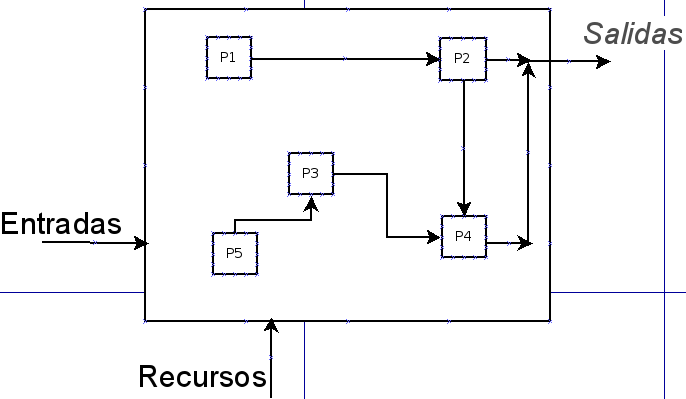
\includegraphics{Organizacion.png}
\end{quote}
\begin{quote}\begin{description}
\item[{Figura1}] \leavevmode
Organización de trabajo.

\end{description}\end{quote}
\end{quote}
\end{quote}


\chapter{\index{Motivación y objetivos}Motivación y objetivos}
\label{_templates/Contenido1/Introduccion:motivacion-y-objetivos}\begin{quote}

Pysafet surge como idea de Fundacite y sucede para complementar la infraestructura de firma electrónica.

Se planteaba como un \textbf{``motor de flujos de trabajo''.}

La construcción de un motor de flujo de trabajo es compleja, hay dos modelos teóricos:
\begin{itemize}
\item {} 
\textbf{BPMN:} Extensión UML comunicar y como segundo objetivo implementar y calcular.

\item {} 
\textbf{Redes de petri:} Calcular y segundo objetivos comunican.

\end{itemize}
\end{quote}


\chapter{Ejemplos de algunos Diagrama de flujo de trabajo}
\label{_templates/Contenido1/Introduccion:ejemplos-de-algunos-diagrama-de-flujo-de-trabajo}\begin{quote}

Todo proceso puede modelarse como un flujo de trabajo. Se hace necesario identificar \textbf{``Eventos'',''Estado'',''Fichas'',''Recursos'',} \textbf{``Dependencias'',''Roles'',''Patrones'',''Mensajes''.}
\begin{itemize}
\item {} 
\textbf{Eventos:} Posible hecho que cambia de estado es una ficha.

\item {} 
\textbf{Estado:} Lugar donde reside una ficha.

\item {} 
\textbf{Ficha:} Documento único dentro del proceso(puede cambiar de datos durante el cambio de estado, pero puede mantener un enlace o \textbf{id} único).

\item {} 
\textbf{Recursos:} Lo que necesita el proceso para funcionar.

\item {} 
\textbf{Roles:} Identidades (digitales) como posible o responsabilidades en los activos de información.

\item {} 
\textbf{Patrones:} Compuestos de modelos generales o recurrentes en los procesos.

\item {} 
\textbf{Mensajes:} Información sobre el a contecer de un evento dirigido a un rol externo (generalmente).

\end{itemize}
\begin{quote}\begin{description}
\item[{Ejemplos  de flujo de trabajo}] \leavevmode
\end{description}\end{quote}

\textbf{1.- Ejemplo:} Solicitar un permiso (gráfico safet y petrii)
\begin{quote}
\begin{itemize}
\item {} 
\textbf{Gráfico usando PySafet}

\end{itemize}

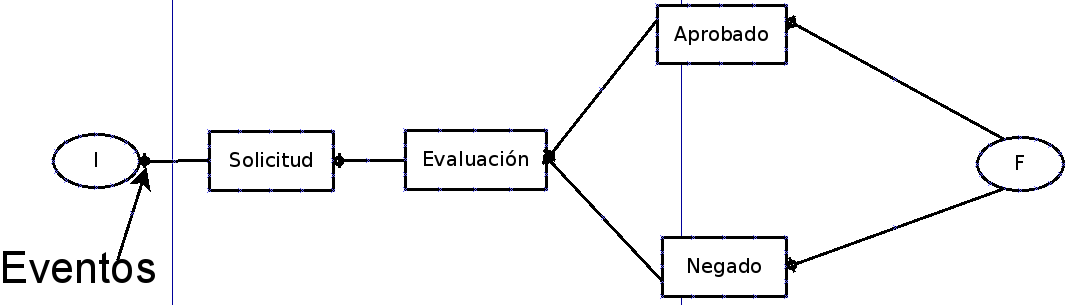
\includegraphics{Diagrama_Pysafe.png}
\begin{quote}\begin{description}
\item[{Figura 2}] \leavevmode
PySafet.

\end{description}\end{quote}

\textbf{Ejercicio:} Determinar Estado,eventos,fichas,dependencias,recursos y roles
\begin{itemize}
\item {} 
\textbf{Gráfico usando Petrii}

\end{itemize}

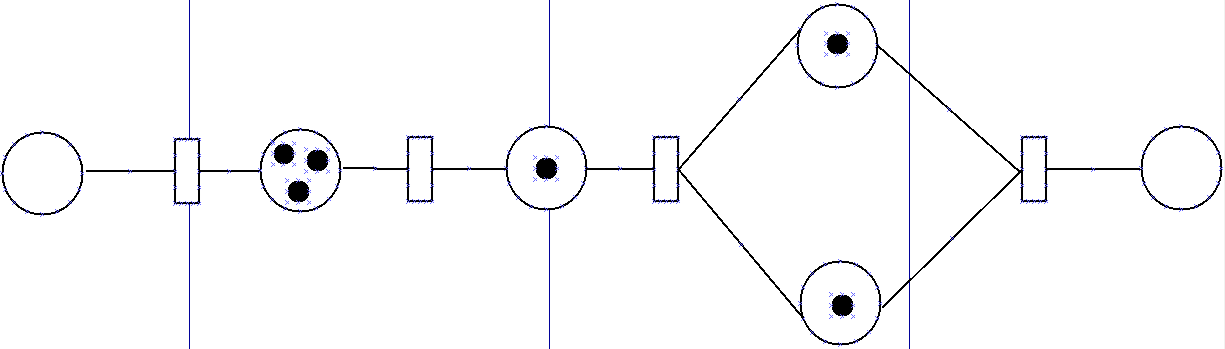
\includegraphics{Diagrama_Petrii.png}
\begin{quote}\begin{description}
\item[{Figura 3}] \leavevmode
Petrii.

\end{description}\end{quote}

\textbf{Ejercicio:} Identificar eventos, estados, dependencias, roles,patrones,mensajes.
\end{quote}

\textbf{2.- Ejemplo:} Caja de ahorro.
\begin{quote}

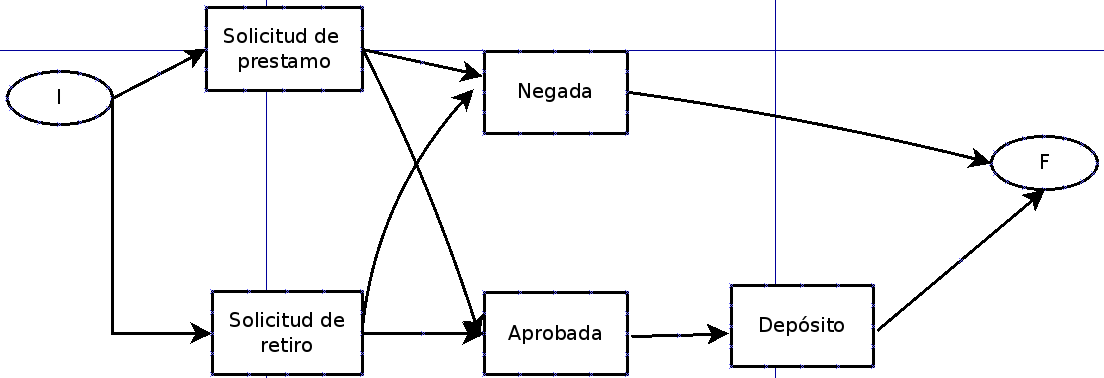
\includegraphics{Caja_ahorro.png}
\begin{quote}\begin{description}
\item[{Figura 4}] \leavevmode
Caja de ahorro.

\end{description}\end{quote}
\end{quote}

\textbf{3.- Ejemplo:} Hola mundo PySafet.
\begin{quote}

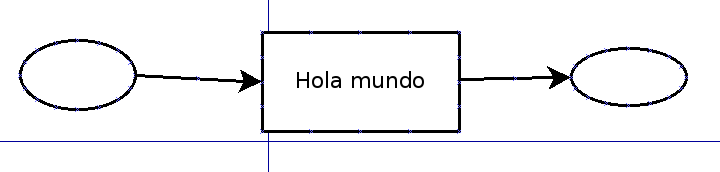
\includegraphics{mundo.png}
\begin{quote}\begin{description}
\item[{Figura5}] \leavevmode
Inicio de PySafet.

\end{description}\end{quote}
\end{quote}
\end{quote}


\chapter{\index{Arquitectura}Arquitectura}
\label{_templates/Contenido1/Introduccion:arquitectura}\begin{quote}

Un motor de flujo de trabajo tiene como principal objetivo calcular (los) el siguiente estado(s) disponibles para la ficha.
\begin{itemize}
\item {} \begin{description}
\item[{\textbf{Se agregan:}}] \leavevmode\begin{enumerate}
\item {} 
Visualización.

\item {} 
Reporte y tiempos.

\item {} 
Validación de estados.

\end{enumerate}

\end{description}

\end{itemize}
\end{quote}


\chapter{\index{Sistema Automatizado de Firma Electrónica y Estampado Electrónico}Sistema Automatizado de Firma Electrónica y Estampado Electrónico}
\label{_templates/Contenido1/Introduccion:sistema-automatizado-de-firma-electronica-y-estampado-electronico}\begin{quote}

Es una herramienta que permite desarrollar nuevas aplicaciones de software con flujos de trabajo, es decir, automatización de forma expedita de procesos de una organización, agregando firma Electrónica y estampillado de tiempo.

La firma electrónica tiene un soporte legal en la Ley sobre Mensajes de Datos y Firma Electrónica (2001) de la República Bolivariana de Venezuela.

El sistema automatizado para la Firma Electrónica y Estampado de Tiempo (SAFET) surge como una herramienta que permite desarrollar nuevas aplicaciones de software que incluyan las funcionalidad de flujos de trabajo, firma Electrónica y estampillado de tiempo.
\end{quote}

\textbf{2.- Instalación}


\chapter{\index{Debian Wheezy 7.0 (64 bits/32bits)}Debian Wheezy 7.0 (64 bits/32bits)}
\label{_templates/Contenido1/Safet_para_Debian::doc}\label{_templates/Contenido1/Safet_para_Debian:debian-wheezy-7-0-64-bits-32bits}\begin{itemize}
\item {} \begin{quote}\begin{description}
\item[{Se Agrega el repositorio al archivo}] \leavevmode
\href{http://linuxgnublog.org/como-anadir-repositorios-en-debian}{/etc/apt/sources.list}

\end{description}\end{quote}

\end{itemize}
\begin{quote}

\begin{Verbatim}[commandchars=\\\{\}]
deb http://tibisay.cenditel.gob.ve/repositorio wheezy main
\end{Verbatim}
\end{quote}
\begin{itemize}
\item {} \begin{quote}\begin{description}
\item[{Obtener la clave}] \leavevmode
\href{http://www.genbetadev.com/seguridad-informatica/manual-de-gpg-cifra-y-envia-datos-de-forma-segura}{(GPG)}

\end{description}\end{quote}

\end{itemize}
\begin{quote}\begin{description}
\item[{del repositorio Debían, utilizando la siguiente línea de comando}] \leavevmode
\begin{Verbatim}[commandchars=\\\{\}]
\PYG{c}{\PYGZsh{} wget http://tibisay.cenditel.gob.ve/repositorio/apt\PYGZhy{}seguridad.gpg.asc}
\PYG{c}{\PYGZsh{} apt\PYGZhy{}key add apt\PYGZhy{}seguridad.gpg.asc}
\end{Verbatim}

\end{description}\end{quote}
\begin{itemize}
\item {} \begin{quote}\begin{description}
\item[{Luego ejecutamos}] \leavevmode
\end{description}\end{quote}

\end{itemize}
\begin{quote}

\begin{Verbatim}[commandchars=\\\{\}]
\PYG{c}{\PYGZsh{} aptitude update}
\PYG{c}{\PYGZsh{} aptitude install pysafet}
\end{Verbatim}
\end{quote}

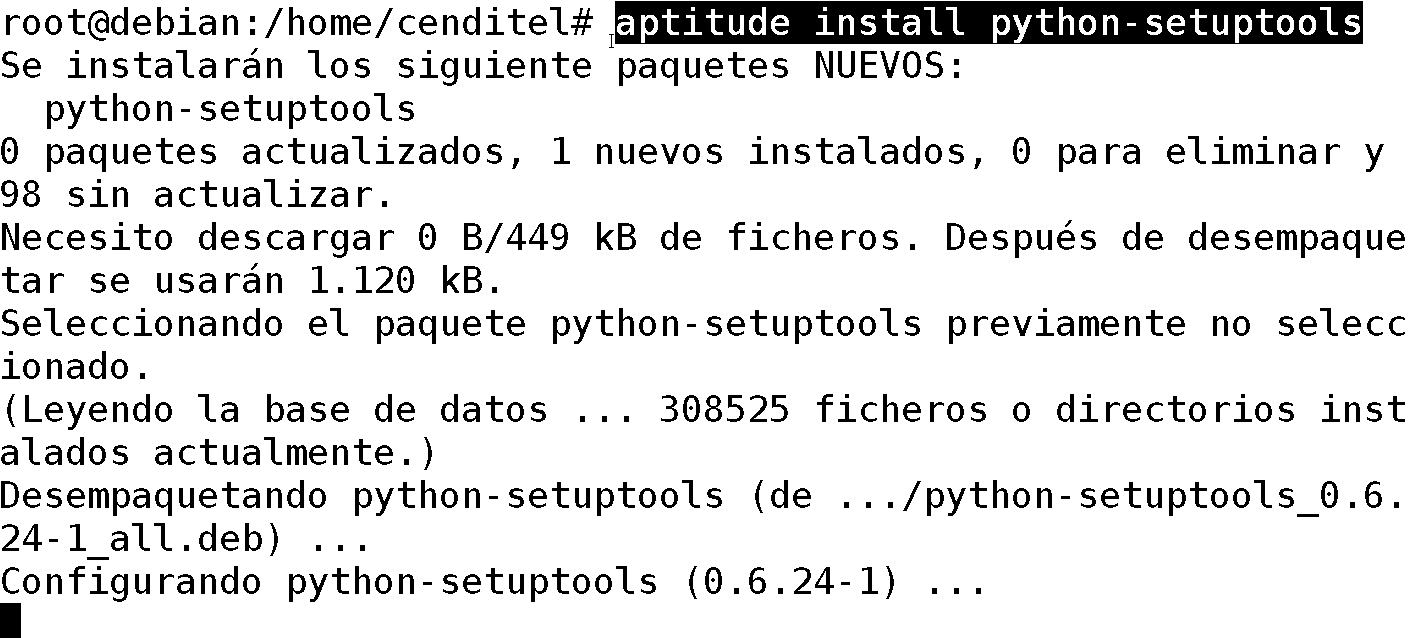
\includegraphics{Pysafet.png}
\begin{quote}\begin{description}
\item[{Figura 6}] \leavevmode
Instalación de pysafet.

\end{description}\end{quote}


\section{\index{Funciones}Funciones}
\label{_templates/Contenido1/Safet_para_Debian:funciones}\begin{itemize}
\item {} \begin{quote}\begin{description}
\item[{Importación}] \leavevmode
Dentro de la consola de python importamos safet para su uso

\end{description}\end{quote}

\begin{Verbatim}[commandchars=\\\{\}]
\PYG{g+gp}{\PYGZgt{}\PYGZgt{}\PYGZgt{} }\PYG{k+kn}{import} \PYG{n+nn}{Safet}
\PYG{g+gp}{\PYGZgt{}\PYGZgt{}\PYGZgt{} }\PYG{n+nb}{dir}\PYG{p}{(}\PYG{n}{Safet}\PYG{p}{)}
\PYG{g+go}{[\PYGZsq{}MainWindow\PYGZsq{}, \PYGZsq{}ParsedSqlToData\PYGZsq{}, \PYGZsq{}SafetDocument\PYGZsq{}, \PYGZsq{}SafetVariable\PYGZsq{}, \PYGZsq{}SafetWorkflow\PYGZsq{},}
\PYG{g+go}{\PYGZsq{}SafetXmlObject\PYGZsq{}, \PYGZsq{}SafetYAWL\PYGZsq{}, \PYGZsq{}\PYGZus{}\PYGZus{}doc\PYGZus{}\PYGZus{}\PYGZsq{}, \PYGZsq{}\PYGZus{}\PYGZus{}file\PYGZus{}\PYGZus{}\PYGZsq{}, \PYGZsq{}\PYGZus{}\PYGZus{}name\PYGZus{}\PYGZus{}\PYGZsq{}, \PYGZsq{}\PYGZus{}\PYGZus{}package\PYGZus{}\PYGZus{}\PYGZsq{}]}
\end{Verbatim}

\item {} \begin{quote}\begin{description}
\item[{Otra formar de mostrar las funciones}] \leavevmode
\end{description}\end{quote}

\begin{Verbatim}[commandchars=\\\{\}]
\PYG{g+gp}{\PYGZgt{}\PYGZgt{}\PYGZgt{} }\PYG{k}{for} \PYG{n}{i} \PYG{o+ow}{in} \PYG{n+nb}{range}\PYG{p}{(}\PYG{n+nb}{len}\PYG{p}{(}\PYG{n+nb}{dir}\PYG{p}{(}\PYG{n}{Safet}\PYG{p}{)}\PYG{p}{)}\PYG{p}{)}\PYG{p}{:}
\PYG{g+gp}{... }    \PYG{n+nb}{dir}\PYG{p}{(}\PYG{n}{Safet}\PYG{p}{)}\PYG{p}{[}\PYG{n}{i}\PYG{p}{]}
\PYG{g+gp}{...}
\PYG{g+go}{\PYGZsq{}MainWindow\PYGZsq{}}
\PYG{g+go}{\PYGZsq{}ParsedSqlToData\PYGZsq{}}
\PYG{g+go}{\PYGZsq{}SafetDocument\PYGZsq{}}
\PYG{g+go}{\PYGZsq{}SafetVariable\PYGZsq{}}
\PYG{g+go}{\PYGZsq{}SafetWorkflow\PYGZsq{}}
\PYG{g+go}{\PYGZsq{}SafetXmlObject\PYGZsq{}}
\PYG{g+go}{\PYGZsq{}SafetYAWL\PYGZsq{}}
\PYG{g+go}{\PYGZsq{}\PYGZus{}\PYGZus{}doc\PYGZus{}\PYGZus{}\PYGZsq{}}
\PYG{g+go}{\PYGZsq{}\PYGZus{}\PYGZus{}file\PYGZus{}\PYGZus{}\PYGZsq{}}
\PYG{g+go}{\PYGZsq{}\PYGZus{}\PYGZus{}name\PYGZus{}\PYGZus{}\PYGZsq{}}
\PYG{g+go}{\PYGZsq{}\PYGZus{}\PYGZus{}package\PYGZus{}\PYGZus{}\PYGZsq{}}
\end{Verbatim}

\end{itemize}


\chapter{\index{Ubuntu (32 bits/ 64 bits)}Ubuntu (32 bits/ 64 bits)}
\label{_templates/Contenido1/Safet_para_Ubuntu:ubuntu-32-bits-64-bits}\label{_templates/Contenido1/Safet_para_Ubuntu::doc}

\chapter{\index{Archivos fuentes}Archivos fuentes}
\label{_templates/Contenido1/Dependencias:archivos-fuentes}\label{_templates/Contenido1/Dependencias::doc}\begin{quote}

El código fuente de la librería Libsafet se encuentra alojada en una plataforma de desarrollo colaborativo de software (forja) llamada Github, esta plataforma utiliza como sistema de control de versión el software Git.
\begin{itemize}
\item {} 
Para la compilación se requiere que se instale las siguientes dependencias:

\end{itemize}
\begin{quote}

\begin{Verbatim}[commandchars=\\\{\}]
libgraphviz\PYGZhy{}dev
libtar\PYGZhy{}dev
g++
libglib2.0\PYGZhy{}dev
x11proto\PYGZhy{}xext\PYGZhy{}dev
libqt4\PYGZhy{}dev
libssl\PYGZhy{}dev
make
python\PYGZhy{}qt4\PYGZhy{}sql
python\PYGZhy{}sip\PYGZhy{}dev
python\PYGZhy{}qt4\PYGZhy{}dev
libqt4\PYGZhy{}sql\PYGZhy{}sqlite
\end{Verbatim}
\end{quote}
\end{quote}
\begin{itemize}
\item {} \begin{quote}\begin{description}
\item[{Para instalar las dependencias desde la línea de comando o terminal (puede hacerlo con synaptics)}] \leavevmode
\end{description}\end{quote}

\end{itemize}
\begin{quote}

\begin{Verbatim}[commandchars=\\\{\}]
\PYGZsh{} aptitude install libgraphviz\PYGZhy{}dev libtar\PYGZhy{}dev g++ libglib2.0\PYGZhy{}dev x11proto\PYGZhy{}xext\PYGZhy{}dev
          libqt4\PYGZhy{}dev libssl\PYGZhy{}dev make python\PYGZhy{}qt4\PYGZhy{}sql python\PYGZhy{}sip\PYGZhy{}dev python\PYGZhy{}qt4\PYGZhy{}dev libqt4\PYGZhy{}sql\PYGZhy{}sqlite
\end{Verbatim}
\end{quote}
\begin{itemize}
\item {} \begin{quote}\begin{description}
\item[{Para clonar el repositorio de Libsafet debemos instalar el control de versiones git}] \leavevmode
\end{description}\end{quote}

\end{itemize}
\begin{quote}

\begin{Verbatim}[commandchars=\\\{\}]
\PYGZdl{} sudo aptitude install git
\end{Verbatim}
\end{quote}
\begin{itemize}
\item {} \begin{quote}\begin{description}
\item[{Luego ubicado en el directorio de trabajo (donde se va a descargar los fuentes) ejecuta el comando}] \leavevmode
\end{description}\end{quote}

\end{itemize}
\begin{quote}

\begin{Verbatim}[commandchars=\\\{\}]
\PYGZdl{} git clone https://github.com/victorrbravo/pysafet.git pysafet

 Dentro del directorio de trabajo se crea el directorio pysafet donde se tiene
el clone de la librería Libsafet
\end{Verbatim}
\end{quote}


\section{\index{Pasos para la compilación}Pasos para la compilación}
\label{_templates/Contenido1/Dependencias:pasos-para-la-compilacion}\begin{itemize}
\item {} \begin{quote}\begin{description}
\item[{Compilación de la libraría Libsafet}] \leavevmode
\end{description}\end{quote}

\end{itemize}
\begin{quote}

\begin{Verbatim}[commandchars=\\\{\}]
\PYGZdl{} cd pysafet/websafet
\PYGZdl{} make clean
\PYGZdl{} qmake\PYGZhy{}qt4
\PYGZdl{} make
\PYGZdl{} cd ../PySafet/
\PYGZdl{}  python configure.py
\PYGZdl{} make
\PYGZdl{} sudo make install
\PYGZdl{} cd ../websafet
\PYGZdl{} sudo make install
\end{Verbatim}
\end{quote}


\section{\index{Verificación de la instalación}Verificación de la instalación}
\label{_templates/Contenido1/Dependencias:verificacion-de-la-instalacion}\begin{itemize}
\item {} \begin{quote}\begin{description}
\item[{Se procede arrancar un interprete de Python, para la misma debe hacer los siguientes paso}] \leavevmode
\end{description}\end{quote}

\end{itemize}
\begin{quote}

\begin{Verbatim}[commandchars=\\\{\}]
\PYGZdl{} python
cenditel@CENDITEL:\PYGZti{}/proyecto/pysafet/websafet\PYGZdl{} python
Python 2.7.3 (default, Jan  2 2013, 13:56:14)
[GCC 4.7.2] on linux2
Type \PYGZdq{}help\PYGZdq{}, \PYGZdq{}copyright\PYGZdq{}, \PYGZdq{}credits\PYGZdq{} or \PYGZdq{}license\PYGZdq{} for more information.
\PYGZgt{}\PYGZgt{}\PYGZgt{}
\end{Verbatim}
\end{quote}
\begin{itemize}
\item {} \begin{quote}\begin{description}
\item[{Dentro prompt de python (\textgreater{}\textgreater{}\textgreater{}), se importa la librería de Safet ejecutando el siguiente comando}] \leavevmode
\end{description}\end{quote}

\begin{Verbatim}[commandchars=\\\{\}]
\PYG{g+gp}{\PYGZgt{}\PYGZgt{}\PYGZgt{} }\PYG{k+kn}{import} \PYG{n+nn}{Safet}
\PYG{g+go}{\PYGZgt{}\PYGZgt{}\PYGZgt{}}
\end{Verbatim}

\end{itemize}


\section{\index{Funciones}Funciones}
\label{_templates/Contenido1/Dependencias:funciones}\begin{itemize}
\item {} 
\begin{Verbatim}[commandchars=\\\{\}]
\PYG{g+gp}{\PYGZgt{}\PYGZgt{}\PYGZgt{} }\PYG{k+kn}{import} \PYG{n+nn}{Safet}
\PYG{g+gp}{\PYGZgt{}\PYGZgt{}\PYGZgt{} }\PYG{n+nb}{dir}\PYG{p}{(}\PYG{n}{Safet}\PYG{p}{)}
\PYG{g+go}{[\PYGZsq{}MainWindow\PYGZsq{}, \PYGZsq{}ParsedSqlToData\PYGZsq{}, \PYGZsq{}SafetDocument\PYGZsq{}, \PYGZsq{}SafetVariable\PYGZsq{}, \PYGZsq{}SafetWorkflow\PYGZsq{},}
\PYG{g+go}{\PYGZsq{}SafetXmlObject\PYGZsq{}, \PYGZsq{}SafetYAWL\PYGZsq{}, \PYGZsq{}\PYGZus{}\PYGZus{}doc\PYGZus{}\PYGZus{}\PYGZsq{}, \PYGZsq{}\PYGZus{}\PYGZus{}file\PYGZus{}\PYGZus{}\PYGZsq{}, \PYGZsq{}\PYGZus{}\PYGZus{}name\PYGZus{}\PYGZus{}\PYGZsq{}, \PYGZsq{}\PYGZus{}\PYGZus{}package\PYGZus{}\PYGZus{}\PYGZsq{}]}
\end{Verbatim}

\end{itemize}

\textbf{3.- Configuración}


\chapter{\index{Paso para la creación del directorio .safet/}Paso para la creación del directorio .safet/}
\label{_templates/Contenido1/Pysafet_home:paso-para-la-creacion-del-directorio-safet}\label{_templates/Contenido1/Pysafet_home::doc}

\section{1° PRIMER PASO}
\label{_templates/Contenido1/Pysafet_home:primer-paso}\begin{quote}

Descargamos nuestro MensajesVersionInicial con estención .tar
\begin{quote}

\textbf{DOWNLOAD:}


\includegraphics{download.png}

\code{ProductoVersionInicial.TAR}
\end{quote}
\end{quote}


\section{2° SEGUNDO PASO}
\label{_templates/Contenido1/Pysafet_home:segundo-paso}\begin{itemize}
\item {} 
Creamos un directorio con cualquier nombre por ejemplo \textbf{Pysafet} en nuestro \textbf{\textless{}HOME\textgreater{}}

\end{itemize}
\begin{quote}

\begin{Verbatim}[commandchars=\\\{\}]
\PYG{n+nv}{\PYGZdl{} }make \PYG{n+nv}{\PYGZdl{}HOME}/Pysafet
\end{Verbatim}
\end{quote}
\begin{itemize}
\item {} 
Copiamos nuestro archivo \textbf{(.tar)} que descargamos a nuestra carpeta \textbf{\textless{}HOME\textgreater{}Pysafet/}. En este caso se descargo en la carpeta \textbf{``Descargas''}.

\end{itemize}
\begin{quote}

\begin{Verbatim}[commandchars=\\\{\}]
\PYG{n+nv}{\PYGZdl{} }cp Descargas/ProductoVersionInicial.tar \PYG{n+nv}{\PYGZdl{}HOME}/Pysafet/
\end{Verbatim}
\end{quote}
\begin{itemize}
\item {} 
Acedemos a la carpeta Pysafet

\end{itemize}
\begin{quote}

\begin{Verbatim}[commandchars=\\\{\}]
\PYG{n+nv}{\PYGZdl{} }\PYG{n+nb}{cd }Pysafet/
\end{Verbatim}
\end{quote}


\section{3° TERCER PASO}
\label{_templates/Contenido1/Pysafet_home:tercer-paso}\begin{itemize}
\item {} 
Crearemos un archivo \textbf{(.py)} por ejemplo \textbf{``MontarSafet.py''} dentro del directorio \textbf{\textless{}HOME\textgreater{}safe/}:

\end{itemize}
\begin{quote}

\begin{Verbatim}[commandchars=\\\{\}]
Pysafet\PYG{n+nv}{\PYGZdl{} }touch MontarSafet.py
\end{Verbatim}
\end{quote}
\begin{itemize}
\item {} 
Abrimos nuestro archivo \textbf{(MontarSafet.py)} y insertamos el siguiente Script de python:

\end{itemize}
\begin{quote}

\begin{Verbatim}[commandchars=\\\{\}]
\PYG{k+kn}{import} \PYG{n+nn}{Safet}
\PYG{k+kn}{import} \PYG{n+nn}{os}

\PYG{n}{myhome} \PYG{o}{=} \PYG{n}{os}\PYG{o}{.}\PYG{n}{getenv}\PYG{p}{(}\PYG{l+s}{\PYGZdq{}}\PYG{l+s}{HOME}\PYG{l+s}{\PYGZdq{}}\PYG{p}{)}
\PYG{n}{mymedia} \PYG{o}{=} \PYG{n}{myhome} \PYG{o}{+} \PYG{l+s}{\PYGZdq{}}\PYG{l+s}{/tmp}\PYG{l+s}{\PYGZdq{}}
\PYG{n}{myurl} \PYG{o}{=} \PYG{l+s}{\PYGZdq{}}\PYG{l+s}{http://localhost}\PYG{l+s}{\PYGZdq{}}

\PYG{n}{myinflow} \PYG{o}{=} \PYG{n}{Safet}\PYG{o}{.}\PYG{n}{MainWindow}\PYG{p}{(}\PYG{n}{myhome}\PYG{p}{)}

\PYG{n}{myinflow}\PYG{o}{.}\PYG{n}{setMediaPath}\PYG{p}{(}\PYG{n}{mymedia}\PYG{p}{)}
\PYG{n}{myinflow}\PYG{o}{.}\PYG{n}{setHostURL}\PYG{p}{(}\PYG{n}{myurl}\PYG{p}{)}

\PYG{n}{myinflow}\PYG{o}{.}\PYG{n}{doLoadConfiguration}\PYG{p}{(}\PYG{l+s}{\PYGZdq{}}\PYG{l+s}{ProductoVersionInicial.tar}\PYG{l+s}{\PYGZdq{}}\PYG{p}{)}
\end{Verbatim}
\end{quote}
\begin{itemize}
\item {} 
Ejecutamos el archivo \textbf{(MontarSafet.py)} desde al consola comando como usuario normal:

\end{itemize}
\begin{quote}

\begin{Verbatim}[commandchars=\\\{\}]
Pysafe\PYG{n+nv}{\PYGZdl{} }python MontarSafet.py
\end{Verbatim}
\end{quote}
\begin{itemize}
\item {} 
Nos vamos al \textbf{\textless{}HOME\textgreater{}}  a verificar si monto el (.safet/) con el comando \textbf{ls}:

\end{itemize}
\begin{quote}

\begin{Verbatim}[commandchars=\\\{\}]
Pysafet\PYG{n+nv}{\PYGZdl{} }ls \PYG{n+nv}{\PYGZdl{}HOME}/.safet/

auth.conf digidoc.conf flowfiles images log     reports xmlrepository
certs     dtd          graphs    input  mydb.db safet.conf
\end{Verbatim}
\end{quote}


\chapter{\index{Estructura del directorio .safet/}Estructura del directorio .safet/}
\label{_templates/Contenido1/Explicacion_safet:estructura-del-directorio-safet}\label{_templates/Contenido1/Explicacion_safet::doc}\begin{itemize}
\item {} \begin{quote}\begin{description}
\item[{Con el comando (tree) visualizamos}] \leavevmode
\end{description}\end{quote}

\end{itemize}
\begin{quote}

\begin{Verbatim}[commandchars=\\\{\}]
Pysafet\PYGZdl{} tree ../.safe/ \PYGZhy{}d
\end{Verbatim}
\end{quote}

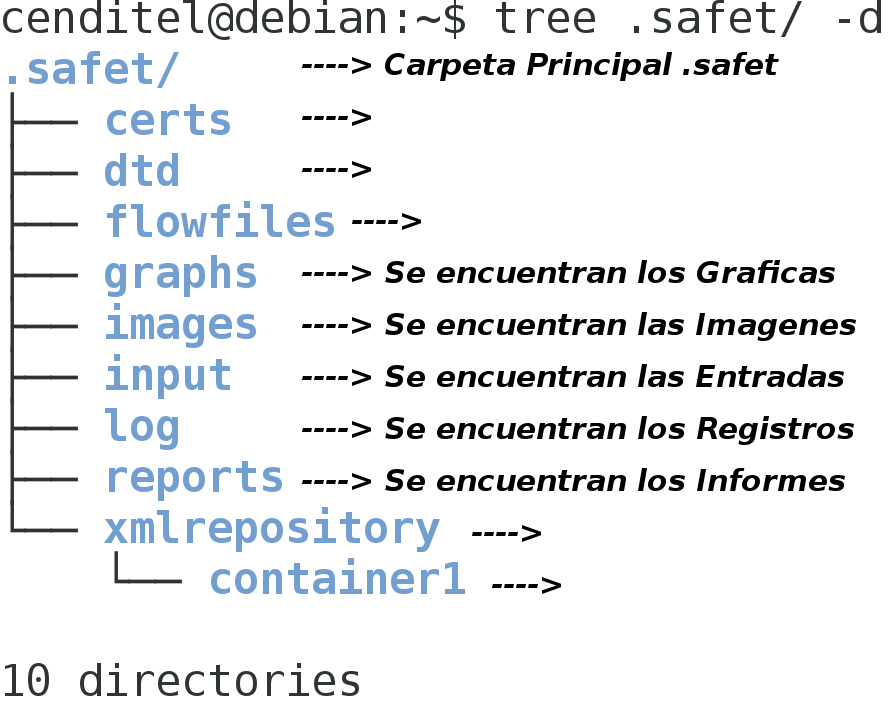
\includegraphics{listasafet.png}
\begin{quote}\begin{description}
\item[{Figura 7}] \leavevmode
Tree.

\end{description}\end{quote}
\begin{itemize}
\item {} \begin{quote}\begin{description}
\item[{Contenido de la carpeta input/}] \leavevmode
\end{description}\end{quote}

\end{itemize}

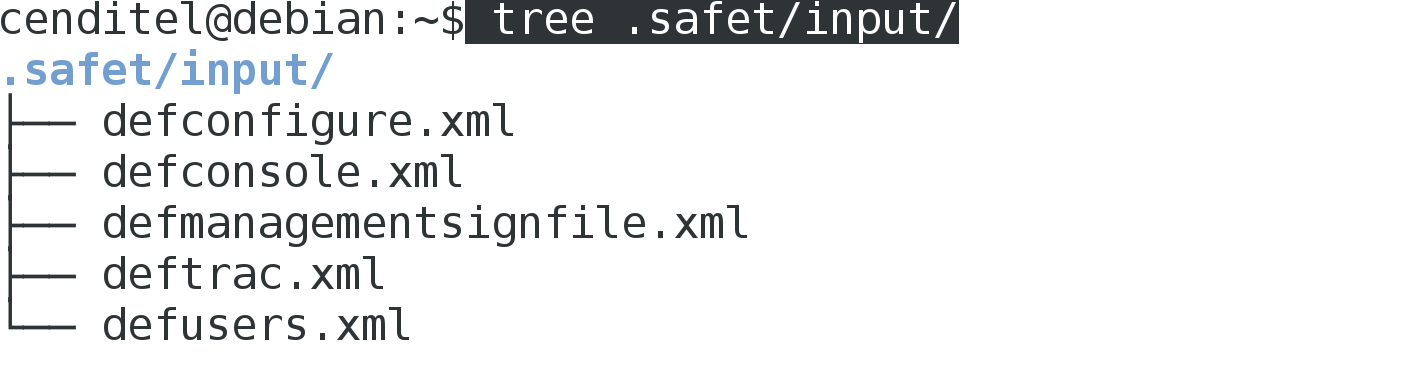
\includegraphics{input.png}
\begin{quote}\begin{description}
\item[{Figura 8}] \leavevmode
Input.

\end{description}\end{quote}

\textbf{4.- Descripción de parámetros del directorio \textless{}HOME\textgreater{}.safet/}


\chapter{\textbf{auth.conf} (Archivo de autenticación y autorización)}
\label{_templates/Contenido2/libsafet_auth_conft:auth-conf-archivo-de-autenticacion-y-autorizacion}\label{_templates/Contenido2/libsafet_auth_conft::doc}\begin{quote}

En este archivo (auth.conf) se especifican los valores de autorización, autenticación y conexión a las base de datos. los Tipo de gestor de base de datos que admitidos

\textbf{database.driver.1 = psql}
\begin{itemize}
\item {} 
Psql : \href{http://www.postgresql.org/}{Postgresql}.

\end{itemize}
\end{quote}
\begin{itemize}
\item {} 
Sqlite : \href{http://www.sqlite.org/}{sqlite3}.

\end{itemize}
\begin{quote}

\textbf{1.- {[}Database{]}:}
\begin{quote}

En esta sección se configura la fuentes de datos. Una fuente de datos esta asociada a una conexión con una base de datos relacional. Es posible tener varias fuentes de datos, cada una representada por un indice.
\end{quote}

\begin{Verbatim}[commandchars=\\\{\}]
[Database]

\PYGZsh{} Información de configuración de fuentes de datos.
\PYGZsh{} Una fuente de datos esta asociada a una conexión con una base
\PYGZsh{} de datos relacional. Es posible tener varias fuentes de datos, cada
\PYGZsh{} una representada por un indice.

\PYGZsh{} Especifica el numero de fuentes de datos diferentes
database.datasources = 1                                \PYGZhy{}\PYGZhy{}\PYGZhy{}\PYGZhy{}\PYGZhy{}\PYGZhy{}\PYGZhy{}\PYGZhy{}\PYGZhy{}\PYGZhy{}\PYGZhy{}\PYGZhy{}\PYGZhy{}\PYGZhy{}\PYGZhy{}\PYGZhy{}\PYGZhy{}\PYGZhy{}\PYGZhy{}\PYGZhy{}\PYGZhy{}\PYGZhy{}\PYGZhy{}\PYGZhy{}\PYGZhy{}\PYGZgt{}Ejemplo: elemento.1 = xxxx, elemento.2 = xxxx
\end{Verbatim}
\begin{quote}\begin{description}
\item[{Note}] \leavevmode
Esté elemento \textbf{(database.datasources)} me indica el número de base de datos, de aquí en adelante todos los elementos que se  requiera estará identificado por el indice asociado a una base de datos.

\end{description}\end{quote}

\begin{Verbatim}[commandchars=\\\{\}]
\PYGZsh{} Para realizar la conexión de base de datos asociada a una fuente de datos
\PYGZsh{} se requieren varios elementos:

\PYGZsh{} Nombre de la fuente de datos 1
database.sourcename.1 = nombre\PYGZus{}fuente\PYGZus{}datos\PYGZus{}1

\PYGZsh{} Especifica el controlador asociado a la fuente de datos
\PYGZsh{} Tipo de gestor de base de datos admitidos

database.driver.1 = controlador\PYGZus{}fuente\PYGZus{}datos\PYGZus{}1       \PYGZhy{}\PYGZhy{}\PYGZhy{}\PYGZhy{}\PYGZhy{}\PYGZhy{}\PYGZhy{}\PYGZhy{}\PYGZhy{}\PYGZhy{}\PYGZhy{}\PYGZhy{}\PYGZhy{}\PYGZhy{}\PYGZhy{}\PYGZhy{}\PYGZhy{}\PYGZhy{}\PYGZgt{}Ejemplo:  database.driver.1 = psql



\PYGZsh{} Especifica si la fuente de datos esta activa o no
database.actived.1 = on

\PYGZsh{} Especifica el nombre de host para la fuente de datos
database.host.1 = host\PYGZus{}base\PYGZus{}de\PYGZus{}datos                  \PYGZhy{}\PYGZhy{}\PYGZhy{}\PYGZhy{}\PYGZhy{}\PYGZhy{}\PYGZhy{}\PYGZhy{}\PYGZhy{}\PYGZhy{}\PYGZhy{}\PYGZhy{}\PYGZhy{}\PYGZhy{}\PYGZhy{}\PYGZhy{}\PYGZhy{}\PYGZhy{}\PYGZgt{}Ejemplo: 127.0.0.0

\PYGZsh{} Especifica el nombre de la base de datos para la fuente de datos

database.db.1 = nombre\PYGZus{}database .1

\PYGZsh{} Especifica el puerto de conexion para la base de datos
database.port.1 = puerto\PYGZus{}database.1

\PYGZsh{} Especifica el nombre de usuario para la fuente de datos
database.user.1 = usuario\PYGZus{}database.1

\PYGZsh{} Especifica la contrasena de acceso para la fuente de datos
database.password.1 = contrasena\PYGZus{}database.1
\end{Verbatim}
\begin{description}
\item[{\textbf{2.- {[}Roles{]}:}}] \leavevmode
En esta sección se define los roles que se van a utilizar en el sistema, la definición de un rol comprende dos \textbf{(2)} elementos:

\end{description}
\begin{itemize}
\item {} 
\textbf{roles.name.n =} nombre del rol n.

\item {} 
\textbf{roles.description.n =} descripción del rol n.

\end{itemize}

\begin{Verbatim}[commandchars=\\\{\}]
[Roles]

roles.name.1 = Administrador
roles.description.1 = usuario(s) que administra el sistema

roles.name.2 = rol\PYGZus{}1
roles.description.2 = descripción del rol  \PYGZhy{}\PYGZhy{}\PYGZhy{}\PYGZhy{}\PYGZhy{}\PYGZhy{}\PYGZhy{}\PYGZhy{}\PYGZhy{}\PYGZhy{}\PYGZhy{}\PYGZhy{}\PYGZhy{}\PYGZhy{}\PYGZhy{}\PYGZhy{}\PYGZhy{}\PYGZhy{}\PYGZhy{}\PYGZhy{}\PYGZgt{} Ejemplo: Acciones asociadas al grupo o al usuario con el rol\PYGZus{}1

roles.name.3 = rol\PYGZus{}2
roles.description.3 = descripción del rol  \PYGZhy{}\PYGZhy{}\PYGZhy{}\PYGZhy{}\PYGZhy{}\PYGZhy{}\PYGZhy{}\PYGZhy{}\PYGZhy{}\PYGZhy{}\PYGZhy{}\PYGZhy{}\PYGZhy{}\PYGZhy{}\PYGZhy{}\PYGZhy{}\PYGZhy{}\PYGZhy{}\PYGZhy{}\PYGZhy{}\PYGZgt{} Ejemplo: Acciones asociadas al grupo o al usuario con el rol\PYGZus{}2
.
.
.

roles.name.n = rol\PYGZus{}n
roles.description.3 = descripción del rol  \PYGZhy{}\PYGZhy{}\PYGZhy{}\PYGZhy{}\PYGZhy{}\PYGZhy{}\PYGZhy{}\PYGZhy{}\PYGZhy{}\PYGZhy{}\PYGZhy{}\PYGZhy{}\PYGZhy{}\PYGZhy{}\PYGZhy{}\PYGZhy{}\PYGZhy{}\PYGZhy{}\PYGZhy{}\PYGZhy{}\PYGZgt{} Ejemplo: Acciones asociadas al grupo o al usuario con el rol\PYGZus{}n
\end{Verbatim}
\begin{description}
\item[{\textbf{3.- {[}Auth{]}:}}] \leavevmode
En esta sección se agrega los usuarios del sistemas, la definición de un usuario comprende cuatro \textbf{(4)} elementos:

\end{description}
\begin{itemize}
\item {} 
\textbf{auth.account.n =} nombre del usuario n.

\item {} 
\textbf{auth.pass.n =} contrañena del usuario n cifrada en md5.

\item {} 
\textbf{auth.realname =} nombre apellido y correo del usuario n separada por espacio.

\item {} 
\textbf{auth..role.n =} rol del usuario n, este rol debe esta definido en el sección {[}Roles{]}.

\end{itemize}

\begin{Verbatim}[commandchars=\\\{\}]
[Auth]

auth.account.1 = usuario 1            \PYGZhy{}\PYGZhy{}\PYGZhy{}\PYGZhy{}\PYGZhy{}\PYGZhy{}\PYGZhy{}\PYGZhy{}\PYGZhy{}\PYGZhy{}\PYGZhy{}\PYGZhy{}\PYGZhy{}\PYGZhy{}\PYGZhy{}\PYGZhy{}\PYGZhy{}\PYGZhy{}\PYGZhy{}\PYGZhy{}\PYGZhy{}\PYGZhy{}\PYGZhy{}\PYGZhy{}\PYGZhy{}\PYGZhy{}\PYGZhy{}\PYGZhy{}\PYGZhy{}\PYGZhy{}\PYGZhy{}\PYGZhy{}\PYGZhy{}\PYGZhy{}\PYGZhy{}\PYGZhy{}\PYGZhy{}\PYGZhy{}\PYGZgt{} Ejemplo: admin
auth.pass.1 = 0f885ebbc5a6c77dac0c319a7411f6039496f06f        \PYGZhy{}\PYGZhy{}\PYGZhy{}\PYGZhy{}\PYGZhy{}\PYGZhy{}\PYGZhy{}\PYGZhy{}\PYGZhy{}\PYGZhy{}\PYGZhy{}\PYGZhy{}\PYGZhy{}\PYGZhy{}\PYGZgt{} Nota: contraseña del admin en md5
auth.realname.1 = Nombre\PYGZus{}apellido\PYGZus{}usuario1  correo\PYGZus{}usuario1   \PYGZhy{}\PYGZhy{}\PYGZhy{}\PYGZhy{}\PYGZhy{}\PYGZhy{}\PYGZhy{}\PYGZhy{}\PYGZhy{}\PYGZhy{}\PYGZhy{}\PYGZhy{}\PYGZhy{}\PYGZhy{}\PYGZgt{} Ejemplo: admin@mail.com
auth.role.1 = rol del usuario                                 \PYGZhy{}\PYGZhy{}\PYGZhy{}\PYGZhy{}\PYGZhy{}\PYGZhy{}\PYGZhy{}\PYGZhy{}\PYGZhy{}\PYGZhy{}\PYGZhy{}\PYGZhy{}\PYGZhy{}\PYGZhy{}\PYGZgt{} Ejemplo: Administrador

auth.account.2 = usuario1
auth.pass.2 = 22cd2d1c596f4091e248aff0e4aa0d47c84b2b36
auth.realname.2 = Nombre\PYGZus{}apellido\PYGZus{}usuario1 usuario1@mail.com
auth.role.2 = rol del usuario

.
.
.

auth.account.n = usuarion
auth.pass.n = ddc6fdd484d5a71b9619beb8b19a7ea06980d8ff
auth.realname.n = Nombre\PYGZus{}apellido\PYGZus{}usuarion usuarion@mail.com
auth.role.n = Desarrollador
\end{Verbatim}

\textbf{4.- {[}Permises{]}:}
\begin{quote}

En esta sección se van a definir los permisos de los usuarios en función de los roles y acciones que puedan ejecutar en el sistema, la definición de cada permisos comprende cuatro \textbf{(4)} elementos:
\end{quote}
\begin{itemize}
\item {} 
\textbf{permises.operation.n =}  nombre de la operación n a ejecutar (estas acción debe estar definida en el archivo deftrac.xml que mas adelante se explicara).

\item {} 
\textbf{permises.accounts.n =} nombre del o los usuario(s) que ejecutara(n) la operación (esta usuario debe estar definido en la sección {[}Auth{]}). Si son varios usuarios deben estar separados por punto y como (;) \textbf{Ejemplo:} permises.accounts.n = usuario1;usuario2;usuarion.

\item {} 
\textbf{permises.types.3 =} tipo de acción a ejecutar, entre las acciones tenemos: read,execute y modify deben ir separadas por punto y como (;) \textbf{Ejemplo:} permises.types.3 = read;execute;modify.

\item {} 
\textbf{permises.roles.4 =} rol que puede ejecutar esta acción, de esta manera se puede indicar a un grupo de usuarios que tenga un rol en especifico ejecutar la acción sin la necesidad de especificarlo en el elemento \textbf{permises.accounts.n}, los roles debe estar definidos en la sección \textbf{{[}Roles{]}}.

\end{itemize}

\begin{Verbatim}[commandchars=\\\{\}]
[Permises]

permises.operation.1 = operacion\PYGZus{}1
permises.accounts.1 = usuario1;admin
permises.types.1 = read;execute;modify
permises.roles.1 = Administrador;rol\PYGZus{}1;rol\PYGZus{}2

permises.operation.2 = operación\PYGZus{}2
permises.accounts.2 = admin
permises.types.2 = read;execute;modify
permises.roles.2 = Administrador
.
.
.
permises.operation.n = operacion\PYGZus{}n
permises.accounts.n = admin
permises.types.n = read;execute;modify
permises.roles.3 = Administrador;rol\PYGZus{}1;rol\PYGZus{}2

\PYGZsh{} Operaciones de Consulta, Lista de datos y gráficos

permises.operation.24 = Listar\PYGZus{}datos
permises.accounts.24 = admin
permises.types.24 = read;execute;modify
permises.roles.24 = Desarrollador;Administrador


permises.operation.25 = Listar\PYGZus{}datos\PYGZus{}con\PYGZus{}autofiltro
permises.accounts.25 = admin
permises.types.25 = read;execute;modify
permises.roles.25 = Administrador


\PYGZsh{} Viñetas

permises.operation.31 = Formulario
permises.accounts.31 = admin
permises.types.31 = read;execute;modify
permises.roles.31 = Administrador;Desarrollador


permises.operation.32 = Consulta
permises.accounts.32 = admin
permises.types.32 = read;execute;modify
permises.roles.32 = Administrador;Desarrollador
\end{Verbatim}
\end{quote}


\chapter{\textbf{safet.conf} (Archivo de configuración inicial)}
\label{_templates/Contenido2/safet_conf:safet-conf-archivo-de-configuracion-inicial}\label{_templates/Contenido2/safet_conf::doc}\begin{quote}
\begin{quote}

En este archivo se especifican los parámetros generales para el funcionamiento de la librería PySafet.
\end{quote}
\begin{description}
\item[{\textbf{1.- {[}Workflow{]}:} (Sección de flujo de trabjo)}] \leavevmode
En esta sección se define el color del flujo y Sección para la interfaz Web.

\end{description}

\begin{Verbatim}[commandchars=\\\{\}]
[Workflow]

\PYGZsh{} Establece el color por defecto
defaultcolor = white            \PYGZhy{}\PYGZhy{}\PYGZhy{}\PYGZhy{}\PYGZhy{}\PYGZhy{}\PYGZgt{} \PYGZsh{} Admite white,black,blue y formato RGB \PYGZsh{}000000

\PYGZsh{} Establece el color activo
activecolor = white

\PYGZsh{} Establece el color pasivo
traccolor =  white
\end{Verbatim}

\textbf{2.- {[}Operators{]}:} (Operadores de flujo de trabajo)
\begin{quote}

En esta sección se establecen las variables de la imágenes de los operadores que son definido en un flujo de trabajo, entre las variables se encuentra:
\end{quote}
\begin{itemize}
\item {} 
\textbf{split.xor =} Se activa un enlace saliente una vez terminada la tarea.

\item {} 
\textbf{split.and =} Activa todos los vínculos salientes una vez terminada esta tarea

\item {} 
\textbf{split.or =} Se utiliza para desencadenar algunos, pero no necesariamente todos los flujos salientes a otras tareas.

\item {} 
\textbf{join.xor =} Esta tarea se activa cada vez que un nuevo enlace se ha activado.

\item {} 
\textbf{join.and =} Esta tarea se activa cuando todos los vínculos se han activado.

\item {} 
\textbf{join.or =} Esta tarea se activa cuando almeno un vinculo se ha activado.

\end{itemize}

\begin{Verbatim}[commandchars=\\\{\}]
[Operators]

\PYGZsh{} Operador split.xor
split.xor = imgs/xor.png   \PYGZhy{}\PYGZhy{}\PYGZhy{}\PYGZhy{}\PYGZhy{}\PYGZgt{} \PYGZsh{} Archivo de imagen en el directorio \PYGZlt{}HOME\PYGZgt{}.safet/imgs

\PYGZsh{} Operador split.and
split.and = imgs/and.png

\PYGZsh{} Operador split.or
split.or = imgs/or.png

\PYGZsh{} Operador join.xor
join.xor = imgs/join\PYGZhy{}xor.png

\PYGZsh{} Operador join.and
join.and = imgs/join\PYGZhy{}and.png

\PYGZsh{} Operador join.or
join.or = imgs/join\PYGZhy{}or.png

\PYGZsh{} Ningun operador
none =  imgs/none.png
\end{Verbatim}

\textbf{3.- {[}Log{]}:} (Registro de eventos)
\begin{quote}

En esta sección se configura las diferentes opciones de la información sobre el registro de los eventos. Entre las opciones tenemos:
\end{quote}
\begin{itemize}
\item {} 
\textbf{log.filepath =} Establece la ruta absoluta donde reside el archivo de registro ejemplo: \textless{}HOME\textgreater{}.safet/.log

\item {} 
\textbf{log.debug =} Habilita la opción de registro de mensajes de depuración (on/off)

\item {} 
\textbf{log.action =} Habilita la opción de registro de de mensajes de acciones (on/off)

\item {} 
\textbf{log.warning =} Habilita la opción de registro de de mensajes de advertencia  (on/off)

\item {} 
\textbf{log.error =} Habilita la opción de registro de de mensajes de error (on/off)

\item {} 
\textbf{log.output =} Salida del registro de ejecución, las opciones son: default (file), file y screen para pantalla.

\end{itemize}

\begin{Verbatim}[commandchars=\\\{\}]
[Log]

\PYGZsh{} Establece la ruta absoluta donde reside el archivo de registro
log.filepath = /home/pbuitrago/.safet/log

\PYGZsh{} Habilita la opción de registro de mensajes de depuración
log.debug = on

\PYGZsh{} Habilita la opción de registro de mensajes de acciones
log.action = on

\PYGZsh{} Habilita la opción de registro de mensajes de advertencia
log.warning = on

\PYGZsh{} Habilita la opción de registro de mensajes de error
log.error = on

\PYGZsh{} Salida del registro de ejecución, las opciones son: default (file), file y screen
log.output = file
\end{Verbatim}

\textbf{4.- {[}XmlRepository{]}:} (Repositorio xml)
\begin{quote}

Información sobre repositorio de documentos firmados electrónica mente bajo el formato \textbf{``bdoc''} (firma electrónica xml) asociados a flujos de trabajos.
\end{quote}

\begin{Verbatim}[commandchars=\\\{\}]
[XmlRepository]
\PYGZsh{} En caso de utilizar un repositorio de documentos XML remoto se debe
\PYGZsh{} especificar la informacion de acceso al mismo a traves de un servicio web
xmlrepository.remote.ip = 150.187.36.6
xmlrepository.remote.urlwebservice = http://150.187.36.6/cgi\PYGZhy{}bin/safet

\PYGZsh{} Establece el tipo de repositorio de documenfet\PYGZus{}auth\PYGZus{}conftos XML. Valores posibles:
\PYGZsh{} dir: para repositorio basado en un directorio local
\PYGZsh{} dbxml: para repositorio DBXML
xmlrepository.type = dir

\PYGZsh{} Establece la ruta absoluta al repositorio XML

xmlrepository.path = \PYGZlt{}HOME\PYGZgt{}.safet/xmlrepository

\PYGZsh{} Establece el nombre del repositorio XML
xmlrepository.name = container1
\end{Verbatim}

\textbf{5.- {[}Input{]}:} (Entrada de datos)
\begin{quote}

Opciones para la entrada/modificación de datos
\end{quote}

\begin{Verbatim}[commandchars=\\\{\}]
[Input]
\PYGZsh{} Establece la ruta absoluta para el directorio en la entrada/modificacion de datos
input.path = \PYGZlt{}HOME\PYGZgt{}.safet/input
\PYGZsh{}input.file = deflista.xml
input.file = deftrac.xml
\end{Verbatim}

\textbf{6.- {[}System{]}:} (Opciones generales para la aplicación Inflow)
\begin{quote}

Opciones generales referentes al funcionamiento del tipo de aplicación : Consola/Web/Gráfica.
\end{quote}

\begin{Verbatim}[commandchars=\\\{\}]
[System]
system.evalexit = on  \PYGZhy{}\PYGZhy{}\PYGZhy{}\PYGZhy{}\PYGZhy{}\PYGZgt{} \PYGZsh{} Preguntar al salir de la aplicación \PYGZdq{}inflow\PYGZdq{}

\PYGZsh{} Información referente a la base de datos o repositorio
\PYGZsh{} para el acceso de la librería
\end{Verbatim}

\textbf{7.- {[}Widgets{]}:} (objetos para entrada de datos)

\begin{Verbatim}[commandchars=\\\{\}]
[Widgets]

\PYGZsh{} Lector de archivo en el sistema
\PYGZsh{} lista de archivos de acceso rápido
widgets.getfilewidget.* = \PYGZlt{}HOME\PYGZgt{}.safet/flowfiles/mensajes.xml


widgets.texteditwidget.wiki.leftbold = \PYGZsq{}\PYGZsq{}\PYGZsq{}              \PYGZhy{}\PYGZhy{}\PYGZhy{}\PYGZgt{} \PYGZsh{} Introducción para el widget \PYGZdq{}wiki\PYGZdq{}
widgets.texteditwidget.wiki.rightbold = \PYGZsq{}\PYGZsq{}\PYGZsq{}                     \PYGZdq{}\PYGZdq{}              \PYGZdq{}\PYGZdq{}        \PYGZdq{}\PYGZdq{}
widgets.texteditwidget.wiki.leftitalic = \PYGZsq{}\PYGZsq{}                     \PYGZdq{}\PYGZdq{}              \PYGZdq{}\PYGZdq{}        \PYGZdq{}\PYGZdq{}
widgets.texteditwidget.wiki.rightitalic = \PYGZsq{}\PYGZsq{}                    \PYGZdq{}\PYGZdq{}              \PYGZdq{}\PYGZdq{}        \PYGZdq{}\PYGZdq{}
widgets.texteditwidget.wiki.leftunderline = \PYGZus{}\PYGZus{}                  \PYGZdq{}\PYGZdq{}              \PYGZdq{}\PYGZdq{}        \PYGZdq{}\PYGZdq{}
widgets.texteditwidget.wiki.rightunderline = \PYGZus{}\PYGZus{}                 \PYGZdq{}\PYGZdq{}              \PYGZdq{}\PYGZdq{}        \PYGZdq{}\PYGZdq{}
\end{Verbatim}

\textbf{8.- {[}GeneralOptions{]}:} (Opciones generales)
\begin{quote}

Esta sección incluye  parámetro de uso generar.
\end{quote}

\begin{Verbatim}[commandchars=\\\{\}]
[GeneralOptions]

generaloptions.consoleactions.* = Gráfico Mensajes;operacion:Generar\PYGZus{}gráfico\PYGZus{}coloreado   \PYGZhy{}\PYGZhy{}\PYGZhy{}\PYGZhy{}\PYGZhy{}\PYGZhy{}\PYGZhy{}\PYGZhy{}\PYGZhy{}\PYGZgt{} \PYGZsh{} Consultas guardadas
Cargar\PYGZus{}archivo\PYGZus{}flujo: \PYGZlt{}HOME\PYGZgt{}.safet/flowfiles/mensajes.xml

generaloptions.consoleactions.* = Grafico por clave;operacion:Generar\PYGZus{}gráfico\PYGZus{}para\PYGZus{}clave
Cargar\PYGZus{}archivo\PYGZus{}flujo: \PYGZlt{}HOME\PYGZgt{}.safet/flowfiles/mensajes.xml Clave: 9      \PYGZhy{}\PYGZhy{}\PYGZhy{}\PYGZhy{}\PYGZhy{}\PYGZhy{}\PYGZhy{}\PYGZhy{}\PYGZhy{}\PYGZgt{} \PYGZsh{} Consultas guardadas

\PYGZsh{} Titulo para el gráfico de flujo de trabajo

generaloptions.currentflowtitle = Tareas Proyecto SAFET

\PYGZsh{} Opciones On (Incluir en el gráfico, No incluir), Off si no se quiere incluir

generaloptions.currentflowtitle.font = Dejavu Sans

\PYGZsh{} Tamaño de la fuente para el texto de informacin en cada flujo de trabajo
generaloptions.currentflowtitle.size = 18

\PYGZsh{} Separación de la fuente para el texto de informacin en cada flujo de trabajo
generaloptions.currentflowtitle.separation = 10

\PYGZsh{} Directorio donde sealmacenan los archivos  de salida grafos(.png,svg)
generaloptions.dir.media = \PYGZlt{}HOME\PYGZgt{}PySafet

generaloptions.currentflowtitle.include = off
\PYGZsh{} Ver http://en.wikipedia.org/wiki/List\PYGZus{}of\PYGZus{}tz\PYGZus{}zones\PYGZus{}by\PYGZus{}name
\PYGZsh{} Zona horaria
generaloptions.timezone = America/Caracas

\PYGZsh{} mostrar información estadística en el grafo
generaloptions.extrainfo.showonly = off
generaloptions.extrainfo.showhumanize = on

\PYGZsh{} Mostrar el dialogo para los parámetros para cada documento de flujo de trabajo

\PYGZsh{} Se colocan las opciones generales del sistema SAFET (Lista de acciones guardadas, entre otros)
\end{Verbatim}

\textbf{9.- {[}Stats{]}:} ( Uso de las estadística para los grafos)
\begin{quote}

Valores para el calculo de estadísticas
\end{quote}

\begin{Verbatim}[commandchars=\\\{\}]
[Stats]

\PYGZsh{}Activar la recolección de estadísticas
stats.actived = off
\PYGZsh{}Fecha de inicio de calculo de estadística, * significa que no hay fecha colocada
stats.fromdate = *
\PYGZsh{}Fecha de fin de calculo de estadística, * significa que no hay fecha colocada
stats.todate = *
\end{Verbatim}

\textbf{10.- {[}Libdigidoc{]}:} (Parámetro para la firma electrónica)
\begin{quote}

Establece variables de configuración para la librería Libdigidoc utilizada por Libsafet.
\end{quote}

\begin{Verbatim}[commandchars=\\\{\}]
[Libdigidoc]
\PYGZsh{} Ruta del archivo de configuración digidoc para usarlo con protocolo OCSP
libdigidoc.configfi:q
lepath = \PYGZlt{}HOME\PYGZgt{}.safet/digidoc.conf

\PYGZsh{} directorio donde se almacenan los certificados de validación
libdigidoc.x509storepath =  \PYGZlt{}HOME\PYGZgt{}.safet/certs

\PYGZsh{} Tipo de validación de firma de Digidoc \PYGZdq{}ocsp\PYGZdq{} : via protocolo OCSP, \PYGZdq{}keystore\PYGZdq{}: Repositorio
\PYGZsh{} de claves del navegador Mozilla / Firefox
\PYGZsh{}libdigidoc.validationtype = keystore

\PYGZsh{} Tipo de archivos \PYGZdq{}MIME\PYGZdq{} permitidos
libdigidoc.mimestypes.* = application/vnd.sun.xml.writer sxw
libdigidoc.mimestypes.* = application/vnd.sun.xml.writer.template stw
libdigidoc.mimestypes.* = application/vnd.sun.xml.writer.global sxg
libdigidoc.mimestypes.* = application/vnd.stardivision.writer sdw vor
libdigidoc.mimestypes.* = application/vnd.stardivision.writer\PYGZhy{}global sgl
libdigidoc.mimestypes.* = application/vnd.sun.xml.calc sxc
libdigidoc.mimestypes.* = application/vnd.sun.xml.calc.template stc
libdigidoc.mimestypes.* = application/vnd.stardivision.calc sdc
libdigidoc.mimestypes.* = application/vnd.sun.xml.impress sxi
libdigidoc.mimestypes.* = application/vnd.sun.xml.impress.template sti
libdigidoc.mimestypes.* = application/vnd.stardivision.impress sdd sdp
libdigidoc.mimestypes.* = application/vnd.sun.xml.draw sxd
libdigidoc.mimestypes.* = application/vnd.sun.xml.draw.template std
libdigidoc.mimestypes.* = application/vnd.stardivision.draw sda
libdigidoc.mimestypes.* = application/vnd.sun.xml.math sxm
libdigidoc.mimestypes.* = application/vnd.stardivision.math smf
libdigidoc.mimestypes.* = application/vnd.oasis.opendocument.text odt
libdigidoc.mimestypes.* = application/vnd.oasis.opendocument.text\PYGZhy{}template ott
libdigidoc.mimestypes.* = application/vnd.oasis.opendocument.text\PYGZhy{}web oth
libdigidoc.mimestypes.* = application/vnd.oasis.opendocument.text\PYGZhy{}master odm
libdigidoc.mimestypes.* = application/vnd.oasis.opendocument.graphics odg
libdigidoc.mimestypes.* = application/vnd.oasis.opendocument.graphics\PYGZhy{}template otg
libdigidoc.mimestypes.* = application/vnd.oasis.opendocument.presentation odp
libdigidoc.mimestypes.* = application/vnd.oasis.opendocument.presentation\PYGZhy{}template otp
libdigidoc.mimestypes.* = application/vnd.oasis.opendocument.spreadsheet ods
libdigidoc.mimestypes.* = application/vnd.oasis.opendocument.spreadsheet\PYGZhy{}template ots
libdigidoc.mimestypes.* = application/vnd.oasis.opendocument.chart odc
libdigidoc.mimestypes.* = application/vnd.oasis.opendocument.formula odf
libdigidoc.mimestypes.* = application/vnd.oasis.opendocument.database odb
libdigidoc.mimestypes.* = application/vnd.oasis.opendocument.image odi
libdigidoc.mimestypes.* = application/pdf pdf
libdigidoc.mimestypes.* = application/xml xml
libdigidoc.mimestypes.* = text/plain txt
libdigidoc.mimestypes.* = text/css css
libdigidoc.mimestypes.* = text/xml xml
libdigidoc.mimestypes.* = text/html html
libdigidoc.mimestypes.* = application/x\PYGZhy{}gzip tgz
libdigidoc.mimestypes.* = application/zip zip
\end{Verbatim}

\textbf{11.- {[}Autofilter{]}:} (Opciones para los Auto filtros)
\begin{quote}

Sirve para realizar clasificaciones automáticas.
\end{quote}

\begin{Verbatim}[commandchars=\\\{\}]
\PYG{p}{[}\PYG{n}{Autofilter}\PYG{p}{]}
\PYG{n}{autofilter}\PYG{o}{.}\PYG{n}{datetime}\PYG{o}{.}\PYG{n}{period} \PYG{o}{=} \PYG{l+m+mi}{672}
\end{Verbatim}

\textbf{12.- {[}DefaultValues{]}:} (Valores por defecto)
\begin{quote}

Opciones que se toman por defecto.
\end{quote}

\begin{Verbatim}[commandchars=\\\{\}]
[DefaultValues]

defaultvalues.report = yes
defaultvalues.digidoc.manifest = Investigador
defaultvalues.digidoc.city = Mérida
defaultvalues.digidoc.state = Mérida
defaultvalues.digidoc.country = VE
defaultvalues.digidoc.zip = 5101
defaultvalues.panel.info.secondstohide = 4000
\end{Verbatim}

\textbf{13.- {[}Reports{]}:} (Reportes)
\begin{quote}

Opcion que es para la generación de reportes.
\end{quote}

\begin{Verbatim}[commandchars=\\\{\}]
[Reports]
\PYGZsh{} Configuraciones para mostrar información en la aplicación Inflow

\PYGZsh{} tipo de protocolo (file,http,ftp,entre otros)
reports.protocol = file

\PYGZsh{} ruta para obtener la plantilla (HTML)
reports.path = \PYGZlt{}HOME\PYGZgt{}.safet/reports

\PYGZsh{} nombre de la plantilla HTML + AJAX
reports.general.template = \PYGZlt{}HOME\PYGZgt{}.safet/reports/sf\PYGZus{}plantillaLista01.html

\PYGZsh{} nombre de la plantilla para documento a firmar
reports.documenttosign.template = \PYGZlt{}HOME\PYGZgt{}.safet/reports/sf\PYGZus{}plantillaFirma01.html

\PYGZsh{} transformar fecha numerica a formato de fecha
reports.options.datetransform = on
reports.options.dateformat = dd/MM/yyyy
\end{Verbatim}

\textbf{14.- {[}Graphs{]}:} (Grafos)
\begin{quote}

Opciones Para los gráficos de flujo de trabajo
\end{quote}

\begin{Verbatim}[commandchars=\\\{\}]
[Graphs]

\PYGZsh{} opciones para el texto de información en cada flujo de trabajo
\PYGZsh{} opciones on/off
graphs.infotext.include = on

\PYGZsh{} Formato  para el texto de informacin en cada flujo de trabajo (el \PYGZpc{}date indica Fecha y \PYGZpc{}time Hora, \PYGZpc{}datetime Hora y Fecha)
graphs.infotext.format = Generado en \PYGZpc{}datetime

\PYGZsh{} Nombre de la fuente para el texto de información en cada flujo de trabajo
graphs.infotext.font = Book Antiqua

\PYGZsh{} Tamaño de la fuente para el texto de información en cada flujo de trabajo
graphs.infotext.size = 14


\PYGZsh{} Separación de la fuente para el texto de información en cada flujo de trabajo
graphs.infotext.separation = 30
\end{Verbatim}

\textbf{15.- {[}Ftp{]}:} (Transferencia FTP)
\begin{quote}

Opción para la trasferencia de archivos utilizando el protocolo \href{http://es.wikipedia.org/wiki/File\_Transfer\_Protocol}{FTP}.
\end{quote}
\end{quote}
\begin{quote}

\begin{Verbatim}[commandchars=\\\{\}]
\PYG{p}{[}\PYG{n}{Ftp}\PYG{p}{]}

\PYG{n}{ftp}\PYG{o}{.}\PYG{n}{default}\PYG{o}{.}\PYG{n}{server} \PYG{o}{=} \PYG{n}{victorbravo}\PYG{o}{.}\PYG{n}{info}
\PYG{n}{ftp}\PYG{o}{.}\PYG{n}{default}\PYG{o}{.}\PYG{n}{account} \PYG{o}{=} \PYG{n}{victorrbravo}
\end{Verbatim}

\textbf{16.- {[}ExtraInfo{]}:} (Información estadísticas de los grafos)
\begin{quote}

Parametros de la información extra de cada nodo
\end{quote}

\begin{Verbatim}[commandchars=\\\{\}]
[ExtraInfo]

extrainfo.infotext.fields = owner,porcentage,completed
extrainfo.infotext.separator =

extrainfo.infotext.completed = [*]

\PYGZsh{} Mostrar campos coloreados (lo ya pasados)
extrainfo.coloured = yes

\PYGZsh{} Mostrar estadísticas al final del grafo (resumen)
extrainfo.summarize = yes

extrainfo.title = Porcentaje:

extrainfo.formula = sumall

extrainfo.pattern = \PYGZsh{}PAR0\PYGZsh{}CLA00\PYGZhy{}9\PYGZsh{}CLA1+\PYGZsh{}PAR1\PYGZsh{}SLA\PYGZpc{}
\end{Verbatim}

\textbf{17.- {[}Plugins{]}:} (Complementos o componentes)
\begin{quote}

Opciones para las librerias adicionales Plugins.
\end{quote}

\begin{Verbatim}[commandchars=\\\{\}]
[Plugins]
\PYGZsh{} Ruta donde se encuentra las librerías adicionales (plugins)
plugins.path = /usr/lib/libsafet
\end{Verbatim}

\textbf{18.- {[}Plugins.Graphviz{]}:} (Componentes Graphviz)
\begin{quote}

Opciónes para la generación de grafos utilizando la biblioteca  \href{http://www.graphviz.org/}{Graphviz}.
\end{quote}
\end{quote}
\begin{quote}

\begin{Verbatim}[commandchars=\\\{\}]
[Plugins.Graphviz]

\PYGZsh{} Formato de archivo de salida de grafo, valores posibles: svg/png/gif
plugins.graphviz.graphtype = svg

\PYGZsh{} Información a mostrar en cuadro de información extra Porc,Tokens,Total,InfoText,InfoDate
plugins.graphviz.extrainfo.show = Porc,Tokens,Total,InfoText,InfoDate


\PYGZsh{}Color activo de para ser utilizado en los gráficos
plugins.graphviz.task.fillcolor = \PYGZsh{}f1f1f1

\PYGZsh{}Color activo de la lnea para ser utilizado en los gráficos
plugins.graphviz.task.color = black


\PYGZsh{} Atributo utilizado en la estadística Opciones posibles (Color/Size/Line/Custom)
plugins.graphviz.stats.attribute = Color

\PYGZsh{} Tamaño máximo para la estadística de (Tamaño Máximo)
plugins.graphviz.stats.sizemax = 2

\PYGZsh{} Tamaño mínimo  para la estadística de (Tamaño Mínimo)
plugins.graphviz.stats.sizemin = 1

\PYGZsh{} Color para dibujar estadística
plugins.graphviz.stats.colorgradient = yellow

\PYGZsh{} Color del texto para cuadro de estadística
plugins.graphviz.stats.fontcolor = black

\PYGZsh{} Color de fondo  para cuadro de estadística
plugins.graphviz.stats.fillcolor = antiquewhite

\PYGZsh{} Estilo de la línea del cuadro de estadística
plugins.graphviz.stats.style = dashed

\PYGZsh{} Mostrar cuadro de estadística
plugins.graphviz.showstats = yes


\PYGZsh{}Dirección del grafo  TB (Arriba\PYGZhy{}Abajo) LR (Izquierda\PYGZhy{}Derecha)
plugins.graphviz.graph.rankdir = TB

\PYGZsh{} Tamao del fuente para todos los nodos
plugins.graphviz.graph.fontsize = 12

\PYGZsh{} Separador del rank
plugins.graphviz.graph.ranksep = 0.5 equally


\PYGZsh{} Figura para la tarea (Task)
plugins.graphviz.task.shape = box

\PYGZsh{} Estilo de la Figura para la tarea (Task) filled,bold,dotted,empty
plugins.graphviz.task.style = filled

\PYGZsh{}Color activo de para ser utilizado en los gráficos
plugins.graphviz.condition.fillcolor = \PYGZsh{}FFFFFF

\PYGZsh{}Color activo de la línea para ser utilizado en los gráficos
plugins.graphviz.condition.color = black

\PYGZsh{} Figura para la (Condition) (box, ellipse, circle, etc.)
plugins.graphviz.condition.shape = ellipse

\PYGZsh{} Estilo de la Figura para la tarea (Condition)
plugins.graphviz.condition.style = filled

\PYGZsh{} Mostrar la información extra solo donde existan tokens (fichas)
plugins.graphviz.extrainfo.showwheretokens = on

\PYGZsh{}Mostrar la estadística en el nodo \PYGZdq{}FINAL\PYGZdq{}, valores admitidos (on/off)
plugins.graphviz.extrainfo.showfinal = on
\end{Verbatim}
\end{quote}

\textbf{5.- API de Safet para el lenguaje de Python}


\chapter{\index{Clase MainWindow(Safet.MainWindow)}Clase MainWindow(Safet.MainWindow)}
\label{_templates/Contenido5/Api:clase-mainwindow-safet-mainwindow}\label{_templates/Contenido5/Api::doc}
\textbf{Clase MainWindow:}
\begin{quote}
\begin{description}
\item[{\textbf{Constructor:}}] \leavevmode\begin{description}
\item[{\textbf{MainWindow} (home-usurio)}] \leavevmode
\textbf{home-usuario:} Directorio del usuario donde se encuentra la carpeta \textbf{.safet/}

\textbf{Ejemplo}

\begin{Verbatim}[commandchars=\\\{\}]
\PYG{g+gp}{\PYGZgt{}\PYGZgt{}\PYGZgt{} }\PYG{k+kn}{import} \PYG{n+nn}{Safet}
\PYG{g+gp}{... }\PYG{k+kn}{import} \PYG{n+nn}{os}
\PYG{g+gp}{... }\PYG{n}{myhome} \PYG{o}{=} \PYG{n}{os}\PYG{o}{.}\PYG{n}{getenv}\PYG{p}{(}\PYG{l+s}{\PYGZdq{}}\PYG{l+s}{HOME}\PYG{l+s}{\PYGZdq{}}\PYG{p}{)}
\PYG{g+gp}{... }\PYG{n}{mymedia} \PYG{o}{=} \PYG{n}{myhome} \PYG{o}{+} \PYG{l+s}{\PYGZdq{}}\PYG{l+s}{/tmp}\PYG{l+s}{\PYGZdq{}}
\PYG{g+gp}{... }\PYG{n}{myurl} \PYG{o}{=} \PYG{l+s}{\PYGZdq{}}\PYG{l+s}{http://localhost}\PYG{l+s}{\PYGZdq{}}
\PYG{g+gp}{...}
\PYG{g+gp}{... }\PYG{n}{myinflow} \PYG{o}{=} \PYG{n}{Safet}\PYG{o}{.}\PYG{n}{MainWindow}\PYG{p}{(}\PYG{n}{myhome}\PYG{p}{)} \PYG{c}{\PYGZsh{}\PYGZhy{}\PYGZhy{}\PYGZhy{}\PYGZgt{} MainWindow}
\end{Verbatim}

\end{description}

\end{description}

\textbf{Listado de myinflow:}
\begin{enumerate}
\item {} \begin{description}
\item[{\textbf{setHostURL} (u) {[}Procedimiento{]}}] \leavevmode
Coloca el url del servidor web actual.

\textbf{Ejemplo:}

\begin{Verbatim}[commandchars=\\\{\}]
\PYG{g+gp}{\PYGZgt{}\PYGZgt{}\PYGZgt{} }\PYG{k+kn}{import} \PYG{n+nn}{Safet}
\PYG{g+gp}{... }\PYG{k+kn}{import} \PYG{n+nn}{os}
\PYG{g+gp}{... }\PYG{n}{myhome} \PYG{o}{=} \PYG{n}{os}\PYG{o}{.}\PYG{n}{getenv}\PYG{p}{(}\PYG{l+s}{\PYGZdq{}}\PYG{l+s}{HOME}\PYG{l+s}{\PYGZdq{}}\PYG{p}{)}
\PYG{g+gp}{... }\PYG{n}{mymedia} \PYG{o}{=} \PYG{n}{myhome} \PYG{o}{+} \PYG{l+s}{\PYGZdq{}}\PYG{l+s}{/tmp}\PYG{l+s}{\PYGZdq{}}
\PYG{g+gp}{... }\PYG{n}{myurl} \PYG{o}{=} \PYG{l+s}{\PYGZdq{}}\PYG{l+s}{http://localhost}\PYG{l+s}{\PYGZdq{}}
\PYG{g+gp}{...}
\PYG{g+gp}{... }\PYG{n}{myinflow} \PYG{o}{=} \PYG{n}{Safet}\PYG{o}{.}\PYG{n}{MainWindow}\PYG{p}{(}\PYG{n}{myhome}\PYG{p}{)}
\PYG{g+gp}{...}
\PYG{g+gp}{... }\PYG{n}{myinflow}\PYG{o}{.}\PYG{n}{setHostURL}\PYG{p}{(}\PYG{n}{myurl}\PYG{p}{)} \PYG{c}{\PYGZsh{}\PYGZhy{}\PYGZhy{}\PYGZhy{}\PYGZgt{} setHostURL}
\end{Verbatim}

\end{description}

\item {} \begin{description}
\item[{\textbf{setMediaPath} (m) {[}Procedimiento{]}}] \leavevmode
Coloca la ruta del directorio de los archivos gráficos.

\textbf{Ejemplo:}

\begin{Verbatim}[commandchars=\\\{\}]
\PYG{g+gp}{\PYGZgt{}\PYGZgt{}\PYGZgt{} }\PYG{k+kn}{import} \PYG{n+nn}{Safet}
\PYG{g+gp}{... }\PYG{k+kn}{import} \PYG{n+nn}{os}
\PYG{g+gp}{... }\PYG{n}{myhome} \PYG{o}{=} \PYG{n}{os}\PYG{o}{.}\PYG{n}{getenv}\PYG{p}{(}\PYG{l+s}{\PYGZdq{}}\PYG{l+s}{HOME}\PYG{l+s}{\PYGZdq{}}\PYG{p}{)}
\PYG{g+gp}{... }\PYG{n}{mymedia} \PYG{o}{=} \PYG{n}{myhome} \PYG{o}{+} \PYG{l+s}{\PYGZdq{}}\PYG{l+s}{/tmp}\PYG{l+s}{\PYGZdq{}}
\PYG{g+gp}{... }\PYG{n}{myurl} \PYG{o}{=} \PYG{l+s}{\PYGZdq{}}\PYG{l+s}{http://localhost}\PYG{l+s}{\PYGZdq{}}
\PYG{g+gp}{...}
\PYG{g+gp}{... }\PYG{n}{myinflow} \PYG{o}{=} \PYG{n}{Safet}\PYG{o}{.}\PYG{n}{MainWindow}\PYG{p}{(}\PYG{n}{myhome}\PYG{p}{)}
\PYG{g+gp}{...}
\PYG{g+gp}{... }\PYG{n}{myinflow}\PYG{o}{.}\PYG{n}{setMediaPath}\PYG{p}{(}\PYG{n}{mymedia}\PYG{p}{)}  \PYG{c}{\PYGZsh{}\PYGZhy{}\PYGZhy{}\PYGZhy{}\PYGZgt{} setMediaPath}
\end{Verbatim}

\end{description}

\item {} \begin{description}
\item[{\textbf{addInfoGraphDateText} () {[}Retorna cadenas (String){]}}] \leavevmode
Agregar la información de fechas al grafo.

\end{description}

\item {} \begin{description}
\item[{\textbf{addNodeToXMLWorkflow} (fname,beforenode = ``'',nodename = ``newnode'',isparallel = false,options'''',query = ``'',nodetitle = ``'',documentsource = ``'') {[}Retorna cadenas (String){]}}] \leavevmode
Agregar un nodo al grafo.

\end{description}

\item {} \begin{description}
\item[{\textbf{autoComplete} (path) {[}Retorna cadenas (String){]}}] \leavevmode
Retorna la lista de autocompletación.

\end{description}

\item {} \begin{description}
\item[{\textbf{changeConnXMLWorkflow} (fname,currnode,nextnode,newnode,newoptions = ``'',newquery ='''' ) {[}Retorna cadenas (String){]}}] \leavevmode
Cambia una conexión entre nodo.

\end{description}

\item {} \begin{description}
\item[{\textbf{checkUserRegister} (fullname,account,email,passone,passtwo) {[}Retorna cadenas (String){]}}] \leavevmode
Realiza el registro de un nuevo usuario.

\end{description}

\item {} \begin{description}
\item[{\textbf{createBdoc} (content) {[}Retorna verdadero si se ejecuto la acción, en caso contrario retorna falso{]}}] \leavevmode
Crea un documento ``bdoc'' vacío.

\end{description}

\item {} \begin{description}
\item[{\textbf{currentDATA} () {[}Retorna cadenas (String){]}}] \leavevmode
Devuelve los datos (DATA) actual.

\end{description}

\item {} \begin{description}
\item[{\textbf{currentError} () {[}Retorna cadenas (String){]}}] \leavevmode
Devuelve el error actual.

\textbf{Ejemplo:}

\begin{Verbatim}[commandchars=\\\{\}]
\PYG{g+gp}{\PYGZgt{}\PYGZgt{}\PYGZgt{} }\PYG{k+kn}{import} \PYG{n+nn}{Safet}
\PYG{g+gp}{... }\PYG{k+kn}{import} \PYG{n+nn}{os}
\PYG{g+gp}{... }\PYG{n}{myhome} \PYG{o}{=} \PYG{n}{os}\PYG{o}{.}\PYG{n}{getenv}\PYG{p}{(}\PYG{l+s}{\PYGZdq{}}\PYG{l+s}{HOME}\PYG{l+s}{\PYGZdq{}}\PYG{p}{)}
\PYG{g+gp}{... }\PYG{n}{mymedia} \PYG{o}{=} \PYG{n}{myhome} \PYG{o}{+} \PYG{l+s}{\PYGZdq{}}\PYG{l+s}{/tmp}\PYG{l+s}{\PYGZdq{}}
\PYG{g+gp}{... }\PYG{n}{myurl} \PYG{o}{=} \PYG{l+s}{\PYGZdq{}}\PYG{l+s}{http://localhost}\PYG{l+s}{\PYGZdq{}}
\PYG{g+gp}{...}
\PYG{g+gp}{... }\PYG{n}{myinflow} \PYG{o}{=} \PYG{n}{Safet}\PYG{o}{.}\PYG{n}{MainWindow}\PYG{p}{(}\PYG{n}{myhome}\PYG{p}{)}
\PYG{g+gp}{... }\PYG{n}{myinflow}\PYG{o}{.}\PYG{n}{setMediaPath}\PYG{p}{(}\PYG{n}{mymedia}\PYG{p}{)}
\PYG{g+gp}{... }\PYG{n}{myinflow}\PYG{o}{.}\PYG{n}{setHostURL}\PYG{p}{(}\PYG{n}{myurl}\PYG{p}{)}
\PYG{g+gp}{...}
\PYG{g+gp}{... }\PYG{n}{myconsult} \PYG{o}{=} \PYG{l+s}{u\PYGZdq{}}\PYG{l+s}{operacion:Listar\PYGZus{}datos Cargar\PYGZus{}archivo\PYGZus{}flujo:/home/cenditel/.safet/flowfiles/mensajes.xml Variable: vIniciado}\PYG{l+s}{\PYGZdq{}}
\PYG{g+gp}{...}
\PYG{g+gp}{... }\PYG{n}{result} \PYG{o}{=} \PYG{n}{myinflow}\PYG{o}{.}\PYG{n}{login}\PYG{p}{(}\PYG{l+s}{\PYGZdq{}}\PYG{l+s}{usuario}\PYG{l+s}{\PYGZdq{}}\PYG{p}{,}\PYG{l+s}{\PYGZdq{}}\PYG{l+s}{usuario}\PYG{l+s}{\PYGZdq{}}\PYG{p}{)}
\PYG{g+gp}{...}
\PYG{g+gp}{... }\PYG{k}{if} \PYG{o+ow}{not} \PYG{n}{result}\PYG{p}{:}
\PYG{g+gp}{... }    \PYG{k}{print} \PYG{l+s}{\PYGZdq{}}\PYG{l+s}{Consult failed error: }\PYG{l+s+si}{\PYGZpc{}s}\PYG{l+s}{\PYGZdq{}}  \PYG{o}{\PYGZpc{}} \PYG{p}{(}\PYG{n}{myinflow}\PYG{o}{.}\PYG{n}{currentError}\PYG{p}{(}\PYG{p}{)}\PYG{p}{)} \PYG{c}{\PYGZsh{}\PYGZsh{}\PYGZsh{}\PYGZhy{}\PYGZhy{}\PYGZhy{}\PYGZhy{}\PYGZgt{}\PYGZgt{}currentError()}
\PYG{g+gp}{... }    \PYG{n+nb}{exit}\PYG{p}{(}\PYG{p}{)}
\end{Verbatim}

\end{description}

\item {} \begin{description}
\item[{\textbf{currentGraphTitle} () {[}Retorna cadenas (String){]}}] \leavevmode
Devuelve  el titulo del último gráfo generado.

\end{description}

\item {} \begin{description}
\item[{\textbf{currentJSON} () {[}Retorna cadenas (String){]}}] \leavevmode
Devuelve la imformación en formato JSON de la última acción generada

\textbf{Ejemplo:}

\begin{Verbatim}[commandchars=\\\{\}]
\PYG{g+gp}{\PYGZgt{}\PYGZgt{}\PYGZgt{} }\PYG{k+kn}{import} \PYG{n+nn}{Safet}
\PYG{g+gp}{... }\PYG{k+kn}{import} \PYG{n+nn}{os}
\PYG{g+gp}{... }\PYG{n}{myhome} \PYG{o}{=} \PYG{n}{os}\PYG{o}{.}\PYG{n}{getenv}\PYG{p}{(}\PYG{l+s}{\PYGZdq{}}\PYG{l+s}{HOME}\PYG{l+s}{\PYGZdq{}}\PYG{p}{)}
\PYG{g+gp}{... }\PYG{n}{mymedia} \PYG{o}{=} \PYG{n}{myhome} \PYG{o}{+} \PYG{l+s}{\PYGZdq{}}\PYG{l+s}{/tmp}\PYG{l+s}{\PYGZdq{}}
\PYG{g+gp}{... }\PYG{n}{myurl} \PYG{o}{=} \PYG{l+s}{\PYGZdq{}}\PYG{l+s}{http://localhost}\PYG{l+s}{\PYGZdq{}}
\PYG{g+gp}{...}
\PYG{g+gp}{... }\PYG{n}{myinflow} \PYG{o}{=} \PYG{n}{Safet}\PYG{o}{.}\PYG{n}{MainWindow}\PYG{p}{(}\PYG{n}{myhome}\PYG{p}{)}
\PYG{g+gp}{... }\PYG{n}{myinflow}\PYG{o}{.}\PYG{n}{setMediaPath}\PYG{p}{(}\PYG{n}{mymedia}\PYG{p}{)}
\PYG{g+gp}{... }\PYG{n}{myinflow}\PYG{o}{.}\PYG{n}{setHostURL}\PYG{p}{(}\PYG{n}{myurl}\PYG{p}{)}
\PYG{g+gp}{...}
\PYG{g+gp}{... }\PYG{n}{myconsult} \PYG{o}{=} \PYG{l+s}{u\PYGZdq{}}\PYG{l+s}{operacion:Listar\PYGZus{}datos Cargar\PYGZus{}archivo\PYGZus{}flujo:/home/cenditel/.safet/flowfiles/mensajes.xml Variable: vIniciado}\PYG{l+s}{\PYGZdq{}}
\PYG{g+gp}{...}
\PYG{g+gp}{... }\PYG{n}{result} \PYG{o}{=} \PYG{n}{myinflow}\PYG{o}{.}\PYG{n}{login}\PYG{p}{(}\PYG{l+s}{\PYGZdq{}}\PYG{l+s}{usuario}\PYG{l+s}{\PYGZdq{}}\PYG{p}{,}\PYG{l+s}{\PYGZdq{}}\PYG{l+s}{usuario}\PYG{l+s}{\PYGZdq{}}\PYG{p}{)}
\PYG{g+gp}{...}
\PYG{g+gp}{... }\PYG{k}{if} \PYG{o+ow}{not} \PYG{n}{result}\PYG{p}{:}
\PYG{g+gp}{... }    \PYG{k}{print} \PYG{l+s}{\PYGZdq{}}\PYG{l+s}{Consult failed error: }\PYG{l+s+si}{\PYGZpc{}s}\PYG{l+s}{\PYGZdq{}}  \PYG{o}{\PYGZpc{}} \PYG{p}{(}\PYG{n}{myinflow}\PYG{o}{.}\PYG{n}{currentError}\PYG{p}{(}\PYG{p}{)}\PYG{p}{)}
\PYG{g+gp}{... }    \PYG{n+nb}{exit}\PYG{p}{(}\PYG{p}{)}
\PYG{g+gp}{...}
\PYG{g+gp}{... }\PYG{k}{print} \PYG{l+s}{u\PYGZdq{}}\PYG{l+s+si}{\PYGZpc{}s}\PYG{l+s}{\PYGZdq{}} \PYG{o}{\PYGZpc{}} \PYG{p}{(}\PYG{n}{myinflow}\PYG{o}{.}\PYG{n}{currentJSON}\PYG{p}{(}\PYG{p}{)}\PYG{p}{)} \PYG{c}{\PYGZsh{}\PYGZsh{}\PYGZsh{}\PYGZhy{}\PYGZhy{}\PYGZhy{}\PYGZhy{}\PYGZgt{}\PYGZgt{}currentJSON()}
\end{Verbatim}

\end{description}

\item {} \begin{description}
\item[{\textbf{currentTable} () {[}Retorna cadenas (String){]}}] \leavevmode
Obtiene los datos en forma de tabla del último gráfo generado.

\end{description}

\item {} \begin{description}
\item[{\textbf{delNodeToXMLWorkflow} (fname,nodename) {[}Retorna cadenas (String){]}}] \leavevmode
Elimina un nodo de un gráfo.

\end{description}

\item {} \begin{description}
\item[{\textbf{doLoadConfiguration} (fileName){[}Procedimiento{]}}] \leavevmode
Carga un archivo de proyecto.

\textbf{Ejemplo}

\begin{Verbatim}[commandchars=\\\{\}]
\PYG{g+gp}{\PYGZgt{}\PYGZgt{}\PYGZgt{} }\PYG{k+kn}{import} \PYG{n+nn}{Safet}
\PYG{g+gp}{... }\PYG{k+kn}{import} \PYG{n+nn}{os}
\PYG{g+gp}{... }\PYG{n}{myhome} \PYG{o}{=} \PYG{n}{os}\PYG{o}{.}\PYG{n}{getenv}\PYG{p}{(}\PYG{l+s}{\PYGZdq{}}\PYG{l+s}{HOME}\PYG{l+s}{\PYGZdq{}}\PYG{p}{)}
\PYG{g+gp}{... }\PYG{n}{mymedia} \PYG{o}{=} \PYG{n}{myhome} \PYG{o}{+} \PYG{l+s}{\PYGZdq{}}\PYG{l+s}{/tmp}\PYG{l+s}{\PYGZdq{}}
\PYG{g+gp}{... }\PYG{n}{myurl} \PYG{o}{=} \PYG{l+s}{\PYGZdq{}}\PYG{l+s}{http://localhost}\PYG{l+s}{\PYGZdq{}}
\PYG{g+gp}{...}
\PYG{g+gp}{... }\PYG{n}{myinflow} \PYG{o}{=} \PYG{n}{Safet}\PYG{o}{.}\PYG{n}{MainWindow}\PYG{p}{(}\PYG{n}{myhome}\PYG{p}{)}
\PYG{g+gp}{...}
\PYG{g+gp}{... }\PYG{n}{myinflow}\PYG{o}{.}\PYG{n}{doLoadConfiguration}\PYG{p}{(}\PYG{l+s}{\PYGZdq{}}\PYG{l+s}{Proyecto.tar}\PYG{l+s}{\PYGZdq{}}\PYG{p}{)}  \PYG{c}{\PYGZsh{}\PYGZsh{}\PYGZsh{}\PYGZhy{}\PYGZhy{}\PYGZhy{}\PYGZhy{}\PYGZgt{}\PYGZgt{} doLoadConfiguration}
\end{Verbatim}

\end{description}

\item {} \begin{description}
\item[{\textbf{doSaveConfiguration} (fileName){[}Procedimiento{]}}] \leavevmode
Guarda un archivo de proyecto (en el directorio \textbf{.safet/} del usuario actual).

\textbf{Ejemplo}

\begin{Verbatim}[commandchars=\\\{\}]
\PYG{g+gp}{\PYGZgt{}\PYGZgt{}\PYGZgt{} }\PYG{k+kn}{import} \PYG{n+nn}{Safet}
\PYG{g+gp}{... }\PYG{k+kn}{import} \PYG{n+nn}{os}
\PYG{g+gp}{... }\PYG{n}{myhome} \PYG{o}{=} \PYG{n}{os}\PYG{o}{.}\PYG{n}{getenv}\PYG{p}{(}\PYG{l+s}{\PYGZdq{}}\PYG{l+s}{HOME}\PYG{l+s}{\PYGZdq{}}\PYG{p}{)}
\PYG{g+gp}{... }\PYG{n}{mymedia} \PYG{o}{=} \PYG{n}{myhome} \PYG{o}{+} \PYG{l+s}{\PYGZdq{}}\PYG{l+s}{/tmp}\PYG{l+s}{\PYGZdq{}}
\PYG{g+gp}{... }\PYG{n}{myurl} \PYG{o}{=} \PYG{l+s}{\PYGZdq{}}\PYG{l+s}{http://localhost}\PYG{l+s}{\PYGZdq{}}
\PYG{g+gp}{...}
\PYG{g+gp}{... }\PYG{n}{myinflow} \PYG{o}{=} \PYG{n}{Safet}\PYG{o}{.}\PYG{n}{MainWindow}\PYG{p}{(}\PYG{n}{myhome}\PYG{p}{)}
\PYG{g+gp}{...}
\PYG{g+gp}{... }\PYG{n}{myinflow}\PYG{o}{.}\PYG{n}{doSaveConfiguration}\PYG{p}{(}\PYG{l+s}{\PYGZdq{}}\PYG{l+s}{usuario.tar}\PYG{l+s}{\PYGZdq{}}\PYG{p}{)} \PYG{c}{\PYGZsh{}\PYGZsh{}\PYGZsh{}\PYGZsh{}\PYGZhy{}\PYGZhy{}\PYGZhy{}\PYGZhy{}\PYGZhy{}\PYGZhy{}\PYGZhy{}\PYGZhy{}\PYGZhy{}\PYGZgt{}\PYGZgt{} doSaveConfiguration}
\end{Verbatim}

\end{description}

\item {} \begin{description}
\item[{\textbf{doSaveGraph} (mypars) {[}Retorna verdadero si se ejecuto la acción, en caso contrario retorna falso{]}}] \leavevmode
Guarda los parámetros de último gráfo generado.

\end{description}

\item {} \begin{description}
\item[{\textbf{generateFormFooter} (o) {[}Retorna cadenas (String){]}}] \leavevmode
Imprime el HTML del pie de pagina general para \textbf{websafet}.

\end{description}

\item {} \begin{description}
\item[{\textbf{generateFormHead} (o) {[}Retorna cadenas (String){]}}] \leavevmode
Imprime el HTML de la cabecera general para \textbf{websafet}.

\end{description}

\item {} \begin{description}
\item[{\textbf{generateModifyHTML} (operation,fieldname,key,secondkey,form) {[}Retorna cadenas (String){]}}] \leavevmode
Genera una consulta \textbf{``AJAX''} para los campos de combos de selección.

\end{description}

\item {} \begin{description}
\item[{\textbf{getFlowParameters} (flowfilename) {[}Retorna cadenas (String){]}}] \leavevmode
Obtiene una lista de parámetros dado un nombre de gráfo.

\end{description}

\item {} \begin{description}
\item[{\textbf{getInfoOfUser} (user) {[}Retorna cadenas (String){]}}] \leavevmode
Obtiene la información de un usuario.

\end{description}

\item {} \begin{description}
\item[{\textbf{hostMediaPath} () {[}Retorna cadenas (String){]}}] \leavevmode
Obtiene la ruta del directorio de archivos multimedia.

\end{description}

\item {} \begin{description}
\item[{\textbf{hostURL} () {[}Retorna cadenas (String){]}}] \leavevmode
Obtiene el url del host \textbf{(websafet)}.

\end{description}

\item {} \begin{description}
\item[{\textbf{inputPath} () {[}Retorna cadenas (String){]}}] \leavevmode
Obtiene el directorio (ruta) de las aplicaciónes actual \textbf{(.safet)}.

\end{description}

\item {} \begin{description}
\item[{\textbf{lastInfoGraph} () {[}Retorna cadenas (String){]}}] \leavevmode
Obtiene información sobre el último gráfo generado.

\end{description}

\item {} \begin{description}
\item[{\textbf{loadReportTemplate} (json,filename = ``'',nameoperation = ``Listar\_datos'') {[}Retorna cadenas (String){]}}] \leavevmode
Carga una plantilla para generar una salida HTML \textbf{(websafet)}.

\end{description}

\item {} \begin{description}
\item[{\textbf{log} (message){[}Procedimiento{]}}] \leavevmode
Escribe en el ``log'' de safet  \textbf{\textless{}HOME\textgreater{}.safet/log/safet.log}.

\end{description}

\item {} \begin{description}
\item[{\textbf{login} (name,pass) {[}Retorna verdadero si se ejecuto la acción, en caso contrario retorna falso{]}}] \leavevmode
Inicia una sesión \textbf{PySafet}.

\textbf{Ejemplo:}

\begin{Verbatim}[commandchars=\\\{\}]
\PYG{g+gp}{\PYGZgt{}\PYGZgt{}\PYGZgt{} }\PYG{k+kn}{import} \PYG{n+nn}{Safet}
\PYG{g+gp}{... }\PYG{k+kn}{import} \PYG{n+nn}{os}
\PYG{g+gp}{... }\PYG{n}{myhome} \PYG{o}{=} \PYG{n}{os}\PYG{o}{.}\PYG{n}{getenv}\PYG{p}{(}\PYG{l+s}{\PYGZdq{}}\PYG{l+s}{HOME}\PYG{l+s}{\PYGZdq{}}\PYG{p}{)}
\PYG{g+gp}{... }\PYG{n}{mymedia} \PYG{o}{=} \PYG{n}{myhome} \PYG{o}{+} \PYG{l+s}{\PYGZdq{}}\PYG{l+s}{/tmp}\PYG{l+s}{\PYGZdq{}}
\PYG{g+gp}{... }\PYG{n}{myurl} \PYG{o}{=} \PYG{l+s}{\PYGZdq{}}\PYG{l+s}{http://localhost}\PYG{l+s}{\PYGZdq{}}
\PYG{g+gp}{...}
\PYG{g+gp}{... }\PYG{n}{myinflow} \PYG{o}{=} \PYG{n}{Safet}\PYG{o}{.}\PYG{n}{MainWindow}\PYG{p}{(}\PYG{n}{myhome}\PYG{p}{)}
\PYG{g+gp}{... }\PYG{n}{myinflow}\PYG{o}{.}\PYG{n}{setMediaPath}\PYG{p}{(}\PYG{n}{mymedia}\PYG{p}{)}
\PYG{g+gp}{... }\PYG{n}{myinflow}\PYG{o}{.}\PYG{n}{setHostURL}\PYG{p}{(}\PYG{n}{myurl}\PYG{p}{)}
\PYG{g+gp}{...}
\PYG{g+gp}{... }\PYG{n}{myconsult} \PYG{o}{=} \PYG{l+s}{u\PYGZdq{}}\PYG{l+s}{operacion:Listar\PYGZus{}datos Cargar\PYGZus{}archivo\PYGZus{}flujo:/home/cenditel/.safet/flowfiles/mensajes.xml Variable: vIniciado}\PYG{l+s}{\PYGZdq{}}
\PYG{g+gp}{...}
\PYG{g+gp}{... }\PYG{n}{result} \PYG{o}{=} \PYG{n}{myinflow}\PYG{o}{.}\PYG{n}{login}\PYG{p}{(}\PYG{l+s}{\PYGZdq{}}\PYG{l+s}{usuario}\PYG{l+s}{\PYGZdq{}}\PYG{p}{,}\PYG{l+s}{\PYGZdq{}}\PYG{l+s}{usuario}\PYG{l+s}{\PYGZdq{}}\PYG{p}{)} \PYG{c}{\PYGZsh{}\PYGZsh{}\PYGZsh{}\PYGZhy{}\PYGZhy{}\PYGZhy{}\PYGZgt{} login}
\end{Verbatim}

\end{description}

\item {} \begin{description}
\item[{\textbf{logout} () {[}Retorna verdadero si se ejecuto la acción, en caso contrario retorna falso{]}}] \leavevmode
Sale una de las sesión \textbf{PySafet}.

\end{description}

\item {} \begin{description}
\item[{\textbf{mediaPath} () {[}Retorna cadenas (String){]}}] \leavevmode
Obtiene las rutas del directorio ``media'' utilizando para generar los gráfos \textbf{(.svg/.png)}.

\end{description}

\item {} \begin{description}
\item[{\textbf{menuCommands} () {[}Retorna cadenas (String){]}}] \leavevmode
Obtiene la lista de acciones en formato HTML.

\end{description}

\item {} \begin{description}
\item[{\textbf{menuForm} (o) {[}Retorna cadenas (String){]}}] \leavevmode
Obtiene un formulario escrito en HTML correspondiente a una acción en el archivo \textbf{\textless{}HOME\textgreater{}.safet/input/deftrac.xml}.

\end{description}

\item {} \begin{description}
\item[{\textbf{postAction} () {[}Retorna cadenas (String){]}}] \leavevmode
Obtiene la acción posterior a ejecutar en uan operación.

\end{description}

\item {} \begin{description}
\item[{\textbf{registerLogin} (user) {[}Procedimiento{]}}] \leavevmode
Escribe en el registro de \textbf{PySafet} el inicio de una seción.

\end{description}

\item {} \begin{description}
\item[{\textbf{registerLogout} (user) {[}Procedimiento{]}}] \leavevmode
Escribe en el registro de \textbf{PySafet} el inicio de la salida de una sesión.

\end{description}

\item {} \begin{description}
\item[{\textbf{sendCheckEmail} (user,plink) {[}Retorna verdadero si se ejecuto la acción, en caso contrario retorna falso{]}}] \leavevmode
Envía un correo de chequeo para el resgistro de un usuario.

\end{description}

\item {} \begin{description}
\item[{\textbf{setConffileValues} (values) {[}Procedimiento{]}}] \leavevmode
Coloca los valores de configuración.

\end{description}

\item {} \begin{description}
\item[{\textbf{setHostMediaPath} (m) {[}Procedimiento{]}}] \leavevmode
Coloca la ruta para los archivo de medias.

\end{description}

\item {} \begin{description}
\item[{\textbf{setTemplatePath} (t) {[}Procedimiento{]}}] \leavevmode
Coloca el directorio de los archivos de plantilla (templates).

\end{description}

\item {} \begin{description}
\item[{\textbf{templatePath} () {[}Retorna cadenas (String){]}}] \leavevmode
Obtiene el directorio para los archivos de plantilla (templates).

\end{description}

\item {} \begin{description}
\item[{\textbf{toInputConsole} (action, withpermises = true) {[}Retorna verdadero si se ejecuto la acción, en caso contrario retorna falso{]}}] \leavevmode
Ejecuta una operación de consulta \textbf{**} en el archivo \textbf{defconsole.xml}.

\textbf{Ejemplo:}

\begin{Verbatim}[commandchars=\\\{\}]
\PYG{g+gp}{\PYGZgt{}\PYGZgt{}\PYGZgt{} }\PYG{k+kn}{import} \PYG{n+nn}{Safet}
\PYG{g+gp}{... }\PYG{k+kn}{import} \PYG{n+nn}{os}
\PYG{g+gp}{... }\PYG{n}{myhome} \PYG{o}{=} \PYG{n}{os}\PYG{o}{.}\PYG{n}{getenv}\PYG{p}{(}\PYG{l+s}{\PYGZdq{}}\PYG{l+s}{HOME}\PYG{l+s}{\PYGZdq{}}\PYG{p}{)}
\PYG{g+gp}{... }\PYG{n}{mymedia} \PYG{o}{=} \PYG{n}{myhome} \PYG{o}{+} \PYG{l+s}{\PYGZdq{}}\PYG{l+s}{/tmp}\PYG{l+s}{\PYGZdq{}}
\PYG{g+gp}{... }\PYG{n}{myurl} \PYG{o}{=} \PYG{l+s}{\PYGZdq{}}\PYG{l+s}{http://localhost}\PYG{l+s}{\PYGZdq{}}
\PYG{g+gp}{...}
\PYG{g+gp}{... }\PYG{n}{myinflow} \PYG{o}{=} \PYG{n}{Safet}\PYG{o}{.}\PYG{n}{MainWindow}\PYG{p}{(}\PYG{n}{myhome}\PYG{p}{)}
\PYG{g+gp}{... }\PYG{n}{myinflow}\PYG{o}{.}\PYG{n}{setMediaPath}\PYG{p}{(}\PYG{n}{mymedia}\PYG{p}{)}
\PYG{g+gp}{... }\PYG{n}{myinflow}\PYG{o}{.}\PYG{n}{setHostURL}\PYG{p}{(}\PYG{n}{myurl}\PYG{p}{)}
\PYG{g+gp}{...}
\PYG{g+gp}{... }\PYG{n}{myconsult} \PYG{o}{=} \PYG{l+s}{u\PYGZdq{}}\PYG{l+s}{operacion:Listar\PYGZus{}datos Cargar\PYGZus{}archivo\PYGZus{}flujo:/home/cenditel/.safet/flowfiles/mensajes.xml Variable: vIniciado}\PYG{l+s}{\PYGZdq{}}
\PYG{g+gp}{...}
\PYG{g+gp}{... }\PYG{n}{result} \PYG{o}{=} \PYG{n}{myinflow}\PYG{o}{.}\PYG{n}{toInputConsole}\PYG{p}{(}\PYG{n}{myconsult}\PYG{p}{)} \PYG{c}{\PYGZsh{}\PYGZsh{}\PYGZsh{}\PYGZhy{}\PYGZhy{}\PYGZhy{}\PYGZhy{}\PYGZhy{}\PYGZhy{}\PYGZgt{}\PYGZgt{}\PYGZgt{} toInputConsole}
\end{Verbatim}

\end{description}

\item {} \begin{description}
\item[{\textbf{toInputForm} (action, withpermises = true) {[}Retorna cadenas (String){]}}] \leavevmode
Ejecuta una operación de entrada de datos (Formulario) descrita en el archivo de \textbf{deftrac.xml}.

\textbf{Ejemplo:}

\begin{Verbatim}[commandchars=\\\{\}]
\PYG{g+gp}{\PYGZgt{}\PYGZgt{}\PYGZgt{} }\PYG{k+kn}{import} \PYG{n+nn}{Safet}
\PYG{g+gp}{... }\PYG{k+kn}{import} \PYG{n+nn}{os}
\PYG{g+gp}{... }\PYG{n}{myhome} \PYG{o}{=} \PYG{n}{os}\PYG{o}{.}\PYG{n}{getenv}\PYG{p}{(}\PYG{l+s}{\PYGZdq{}}\PYG{l+s}{HOME}\PYG{l+s}{\PYGZdq{}}\PYG{p}{)}
\PYG{g+gp}{... }\PYG{n}{mymedia} \PYG{o}{=} \PYG{n}{myhome} \PYG{o}{+} \PYG{l+s}{\PYGZdq{}}\PYG{l+s}{/tmp}\PYG{l+s}{\PYGZdq{}}
\PYG{g+gp}{... }\PYG{n}{myurl} \PYG{o}{=} \PYG{l+s}{\PYGZdq{}}\PYG{l+s}{http://localhost}\PYG{l+s}{\PYGZdq{}}
\PYG{g+gp}{...}
\PYG{g+gp}{... }\PYG{n}{myinflow} \PYG{o}{=} \PYG{n}{Safet}\PYG{o}{.}\PYG{n}{MainWindow}\PYG{p}{(}\PYG{n}{myhome}\PYG{p}{)}
\PYG{g+gp}{... }\PYG{n}{myinflow}\PYG{o}{.}\PYG{n}{setMediaPath}\PYG{p}{(}\PYG{n}{mymedia}\PYG{p}{)}
\PYG{g+gp}{... }\PYG{n}{myinflow}\PYG{o}{.}\PYG{n}{setHostURL}\PYG{p}{(}\PYG{n}{myurl}\PYG{p}{)}
\PYG{g+gp}{...}
\PYG{g+gp}{... }\PYG{n}{myconsult} \PYG{o}{=} \PYG{l+s}{u\PYGZdq{}}\PYG{l+s}{operacion:agregar\PYGZus{}mensaje Titulo: hola mundo}\PYG{l+s}{\PYGZdq{}}
\PYG{g+gp}{...}
\PYG{g+gp}{... }\PYG{n}{result} \PYG{o}{=} \PYG{n}{myinflow}\PYG{o}{.}\PYG{n}{toInputForm}\PYG{p}{(}\PYG{n}{myconsult}\PYG{p}{)} \PYG{c}{\PYGZsh{}\PYGZsh{}\PYGZsh{}\PYGZhy{}\PYGZhy{}\PYGZhy{}\PYGZhy{}\PYGZhy{}\PYGZhy{}\PYGZgt{}\PYGZgt{}\PYGZgt{} toInputForm}
\end{Verbatim}

\end{description}

\item {} \begin{description}
\item[{\textbf{toInputUsers} (action) {[}Retorna verdadero si se ejecuto la acción, en caso contrario retorna falso{]}}] \leavevmode
Ejecuta una acción de gestión de usuarios descrita en el archivo \textbf{defusers.xml}.

\end{description}

\end{enumerate}
\end{quote}


\chapter{\index{Clase SafetXmlObject (Safet.SafetXmlObject)}Clase SafetXmlObject (Safet.SafetXmlObject)}
\label{_templates/Contenido5/Clase2:clase-safetxmlobject-safet-safetxmlobject}\label{_templates/Contenido5/Clase2::doc}
\textbf{Clase SafetXmlObject:}
\begin{quote}
\begin{description}
\item[{\{}] \leavevmode
\%TypeHeaderCode
\#include ''../websafet/src/SafetXmlObject.h''
\%End
\begin{description}
\item[{public:}] \leavevmode
SafetXmlObject();
bool syncAttributes(const QDomElement\&);

\end{description}

\end{description}

\};
\end{quote}


\chapter{\index{Clase SafetDocument}Clase SafetDocument}
\label{_templates/Contenido5/Clase3:clase-safetdocument}\label{_templates/Contenido5/Clase3::doc}\begin{description}
\item[{\textbf{Clase SafetDocument}}] \leavevmode{[}SafetXmlObject{]}
Esta clase modela un documento de una variable en \textbf{PySafet} (el documento puede ser firmado electrónicamente).

\textbf{Listado de myinflow:}
\begin{enumerate}
\item {} \begin{description}
\item[{\textbf{getCertFileList} (ext = ''.pem'') {[}Retorna cadenas (String){]}}] \leavevmode
Obtiene la ruta del certificado usado para firmar el documento.

\end{description}

\item {} \begin{description}
\item[{\textbf{numberOfDataFileOnOpenXAdESContainer} () {[}Retorna un entero (int){]}}] \leavevmode
Número de archivos que contienen el documento firmado.

\end{description}

\item {} \begin{description}
\item[{\textbf{numberOfSignaturesOnOpenXAdESContainer} () {[}Retorna un entero (int){]}}] \leavevmode
Número de firmas que contienen el documento firmado.

\end{description}

\item {} \begin{description}
\item[{\textbf{getDataFileName} (index = 0) {[}Retorna cadenas (String){]}}] \leavevmode
Nombre del archivo contenido de índice ``index''.

\end{description}

\item {} \begin{description}
\item[{\textbf{getDataFileLength} (index = 0) {[}Retorna un (long){]}}] \leavevmode
Tamaño del archivo contenodo de índice ``index''.

\end{description}

\item {} \begin{description}
\item[{\textbf{getDataFileMimeType} (index = 0) {[}Retorna cadenas (String){]}}] \leavevmode
Tipo de archivo contenido de índice ``indice''.

\end{description}

\item {} \begin{description}
\item[{\textbf{numberOfDataFileAttributes} (index = 0) {[}Retorna un entero (int){]}}] \leavevmode
Atributo del archivo contenido de índice ``indice''.

\end{description}

\item {} \begin{description}
\item[{\textbf{getXmlQuery} (query,dcount,info = ``'') {[}Retorna cadenas (String){]}}] \leavevmode
Obtiene consulta \textbf{XML}.

\end{description}

\item {} \begin{description}
\item[{\textbf{addSignatureToExistingDigidocFile} (keyFile,passwd,certFile,inFile,outFile) {[}Retorna un entero (int){]}}] \leavevmode
Agrega un firma al archivo.

\end{description}

\item {} \begin{description}
\item[{\textbf{signWithPrivateKeyOnFile} (keyFile,passwd,certFile,inFile,outFile,manifest,city,state,zip,country,notaryUrl,proxyHost,proxyPort){[}Retorna un entero (int){]}}] \leavevmode
Firma electrónicamente un archivo con un certificado PCKS\#LZ.

\end{description}

\item {} \begin{description}
\item[{\textbf{initPKCS11Lib} (libName) {[}Procedimiento{]}}] \leavevmode
Inicia el manejador de la tarjeta inteligente.

\end{description}

\item {} \begin{description}
\item[{\textbf{initDigidocConfigStore} (configFile) {[}Retorna un entero (int){]}}] \leavevmode
Inicializa la configuración.

\end{description}

\item {} 
\textbf{verifySignMadeWithSmartCard} (fileName) {[}Retorna verdadero si se ejecuto la acción, en caso contrario retorna falso{]}

\item {} 
\textbf{verifySignMadeWithSmartCard} (fileName,signatureIndex)  {[}Retorna verdadero si se ejecuto la acción, en caso contrario retorna falso{]}

\item {} 
\textbf{verifySignMadeWithSmartCard} (fileName,listOfSigners,isneg,op = SafetDocument::AND )  {[}Retorna verdadero si se ejecuto la acción, en caso contrario retorna falso{]}
\begin{quote}

Verifica una firma electrónica que fue realizada utilizando tarjeta inteligente.
\end{quote}

\item {} \begin{description}
\item[{\textbf{testSmartCardDriver} (slot) {[}Procedimiento{]}}] \leavevmode
Realiza una prueba a la conexión con la tarjeta inteligente.

\end{description}

\item {} \begin{description}
\item[{\textbf{getCN} (signatureIndex) {[}Retorna cadenas (String){]}}] \leavevmode
Retorna el nombre común de la firma \textbf{``signature Index'' (commun name)} .

\end{description}

\item {} \begin{description}
\item[{\textbf{getSignerIndex} (cn) {[}Retorna un entero (int){]}}] \leavevmode
Retorna el índice de firma del correspondiente nombre camún (ch).

\end{description}

\item {} \begin{description}
\item[{\textbf{getCommonNameOfSigners} () {[}Retorna cadenas (String){]}}] \leavevmode
Obtiene una lista con el nombre camún de los firmantes del archivo.

\end{description}

\item {} \begin{description}
\item[{\textbf{getNumberOfPrivateKeys} (slot,passwd,libName) {[}Retorna un entero (int){]}}] \leavevmode
Obtiene el número de claves privadas utilizados para el archivo.

\end{description}

\item {} \begin{description}
\item[{\textbf{writeFileToDisk} (string,name) {[}Retorna cadenas (String){]}}] \leavevmode
Escribe en otro archivo el documento.

\end{description}

\item {} \begin{description}
\item[{\textbf{returnFileToString} (pathFileName) {[}Retorna cadenas (String){]}}] \leavevmode
Convierte el archivo a una cadena.

\end{description}

\item {} \begin{description}
\item[{\textbf{decryptDocument} (inFile,outputFile,pin) {[}Retorna un entero (int){]}}] \leavevmode
Descifra (decencripta) el archivo.

\end{description}

\item {} \begin{description}
\item[{\textbf{decryptString} (inFile,pin){[}Retorna cadenas (String){]}}] \leavevmode
Descifra (decencripta) una cadena.

\end{description}

\item {} \begin{description}
\item[{\textbf{getTempNameFiles} (n) {[}Retorna cadenas (String){]}}] \leavevmode
Crea ``n'' archivos temporales.

\end{description}

\item {} \begin{description}
\item[{\textbf{getCommonNameFromCertificate} (certPath) {[}Retorna cadenas (String){]}}] \leavevmode
Obtiene el nombre camún (CN) de un archivo de certificación.

\end{description}

\item {} \begin{description}
\item[{\textbf{getCountryOfSignature} (index = 0) {[}Retorna cadenas (String){]}}] \leavevmode
Obtiene el valor de país \textbf{``country''} especificado para la frima electrónica de índice \textbf{``Index''}.

\end{description}

\item {} \begin{description}
\item[{\textbf{getStateOfSignature} (index = 0) {[}Retorna cadenas (String){]}}] \leavevmode
Obtiene el valor del Estado \textbf{(STATE)} departamento o región especificando para la firma electrónica de índice ``Indice''.

\end{description}

\item {} \begin{description}
\item[{\textbf{getCityOfSignature} (index = 0) {[}Retorna cadenas (String){]}}] \leavevmode
Obtiene el valor de la Ciudad.

\end{description}

\item {} \begin{description}
\item[{\textbf{getPostalCodeOfSignature} (index = 0) {[}Retorna cadenas (String){]}}] \leavevmode
Obtiene el valor de código Postal.

\end{description}

\item {} \begin{description}
\item[{\textbf{getCountOfRoles} (index = 0) {[}Retorna un entero (int){]}}] \leavevmode
Obtiene el número de roles (nominación de cargo del firmante).

\end{description}

\item {} 
\textbf{getRole} (index = 0,roleIndex = 0) {[}Retorna cadenas (String){]}

\item {} 
\textbf{getSingingTime} (index = 0) {[}Retorna cadenas (String){]}

\item {} 
\textbf{getSingingTimeOnlyDate} (index = 0) {[}Retorna cadenas (String){]}

\item {} 
\textbf{getSingingTimeOnlyHour} (index = 0) {[}Retorna cadenas (String){]}

\item {} 
\textbf{getSignatureType} (index = 0) {[}Retorna cadenas (String){]}

\item {} 
\textbf{getSignatureFormat} (index = 0) {[}Retorna cadenas (String){]}

\item {} 
\textbf{getSignerCertificateIssuerName} (index = 0) {[}Retorna cadenas (String){]}

\item {} 
\textbf{getSignerCertificateSerial} (index = 0) {[}Retorna cadenas (String){]}

\item {} 
\textbf{getValidAt} (index = 0) {[}Retorna cadenas (String){]}

\item {} \begin{description}
\item[{\textbf{getValidUntil} (index = 0) {[}Retorna cadenas (String){]}}] \leavevmode
Obtiene datos del certificado electrónico usado para la firma de índice ``Indice''.

\end{description}

\item {} \begin{description}
\item[{\textbf{getPathOfSafetDocument} () {[}Retorna cadenas (String){]}}] \leavevmode
Obtiene la ruta donde se guarda los documentos firmados.

\end{description}

\item {} 
\textbf{setPathOfSafetDocument} (path) {[}Procedimiento{]}

\item {} 
\textbf{getSubjectDN} (index = 0) {[}Retorna cadenas (String){]}

\item {} 
\textbf{getIssuerDN} (index = 0) {[}Retorna cadenas (String){]}

\item {} 
\textbf{policies} (index = 0) {[}Retorna cadenas (String){]}

\item {} 
\textbf{getPublicKeyAlgorithm} (index = 0) {[}Retorna cadenas (String){]}

\item {} 
\textbf{getPublicKeyLength} (index = 0) {[}Retorna cadenas (String){]}

\item {} 
\textbf{writeX509ToFile} (path,PEM,index = 0) {[}Procedimiento{]}

\end{enumerate}

QByteArray versionNumber(int index = 0)

QByteArray serialNumber(int index = 0);

QByteArray toHex( const QByteArray \&in, QChar separator );

QByteArray authorityKeyIdentifier(int index = 0);

QByteArray subjectKeyIdentifier(int index = 0);

\end{description}


\chapter{\index{Clase SafetVariable}Clase SafetVariable}
\label{_templates/Contenido5/Clase4::doc}\label{_templates/Contenido5/Clase4:clase-safetvariable}
\textbf{Clase SafetVariable} : SafetXmlObject
\begin{quote}

\textbf{Listado de myinflow:}
\begin{enumerate}
\item {} 
\textbf{addChild} (SafetXmlObject) {[}Procedimiento{]}

\item {} 
\textbf{id} () {[}Retorna cadenas (String){]}

\item {} 
\textbf{setId} () {[}Procedimiento{]}

\item {} 
\textbf{tokenlink} (s) {[}Retorna cadenas (String){]}

\item {} 
\textbf{setTokenlink} (b) {[}Procedimiento{]}

\item {} 
\textbf{scope} (a) {[}Retorna cadenas (String){]}

\item {} 
\textbf{setScope} (z) {[}Procedimiento{]}

\item {} 
\textbf{type} () {[}Retorna cadenas (String){]}

\item {} 
\textbf{setType} (a) {[}Procedimiento{]}

\item {} 
\textbf{config} () {[}Retorna cadenas (String){]}

\item {} 
\textbf{setConfig} (q) {[}Procedimiento{]}

\item {} 
\textbf{source} () {[}Retorna cadenas (String){]}

\item {} 
\textbf{setSource} (f) {[}Procedimiento{]}

\item {} 
\textbf{documentsource} () {[}Retorna cadenas (String){]}

\item {} 
\textbf{setDocumentsource} (w) {[}Procedimiento{]}

\item {} 
\textbf{description} () {[}Retorna cadenas (String){]}

\item {} 
\textbf{setDescription} (f) {[}Procedimiento{]}

\item {} 
\textbf{foo} () {[}Retorna cadenas (String){]}

\item {} 
\textbf{getDocumentCount} () {[}Retorna un entero (int){]}

\end{enumerate}

QList\textless{}SafetDocument*\textgreater{}\& getDocuments();
\begin{enumerate}
\item {} 
\textbf{getXMLDocument} (value,fieldno,documentid) {[}Retorna cadenas (String){]}

\item {} 
\textbf{createXMLFileFromQuery} (query,outputFileName) {[}Retorna cadenas (String){]}

\end{enumerate}
\end{quote}


\chapter{\index{Clase SafetYAWL}Clase SafetYAWL}
\label{_templates/Contenido5/Clase5:clase-safetyawl}\label{_templates/Contenido5/Clase5::doc}
\textbf{Clase SafetYAWL} : SafetXmlObject
\begin{quote}

\textbf{Listado de myinflow:}
\begin{enumerate}
\item {} 
\textbf{openXML} (a) {[}Procedimiento{]}

\item {} 
\textbf{convertXMLtoObjects} () {[}Procedimiento{]}

\item {} 
\textbf{openDataSources} () {[}Procedimiento{]}

\item {} 
\textbf{setCurrentPin} (p) {[}Procedimiento{]}

\item {} 
\textbf{currentPin} () {[}Retorna cadenas (String){]}

\item {} 
\textbf{signDocumentsFromData} (c,nametowrite,list,doc,withsmartcard = true) {[}Retorna verdadero si se ejecuto la acción, en caso contrario retorna falso{]}

\item {} 
\textbf{verifyDocumentsFromData} (data,doc) {[}Retorna verdadero si se ejecuto la acción, en caso contrario retorna falso{]}

\item {} 
\textbf{loadAllConfFiles} (option = 3) {[}Procedimiento{]}

\item {} 
\textbf{loadPlugins} (plugname) {[}Procedimiento{]}

\end{enumerate}
\end{quote}


\chapter{\index{Clase SafetWorkflow}Clase SafetWorkflow}
\label{_templates/Contenido5/Clase6:clase-safetworkflow}\label{_templates/Contenido5/Clase6::doc}
\textbf{Clase SafetWorkflow: SafetXmlObject}
\begin{quote}

\textbf{Listado de myinflow:}

enum OutputFormat \{ XML, JSON, SVG \};
\begin{enumerate}
\item {} 
\textbf{SafetWorkflow} ()

\item {} 
\textbf{listTasks} (inc = false,c = ``n'') {[}Retorna cadenas (String){]}

\end{enumerate}

//    SafetDocument getDocuments(const QString\& idvariable, OutputFormat of = XML
//                         const QString\& info ='''');

//    SafetDocument getDocuments(const QString\& idvariable, QList\textless{}QSqlField\textgreater{}\& fields,int \&howmanydocuments,
//                         OutputFormat of = XML,
//                         const QString\& info ='''');
\end{quote}

\textbf{6.- Tutorial sobre un ejemplo de sistema de inventario}


\chapter{\index{Creación de las tablas en base de datos}Creación de las tablas en base de datos}
\label{_templates/Contenido6/manual_Parte1:creacion-de-las-tablas-en-base-de-datos}\label{_templates/Contenido6/manual_Parte1::doc}\begin{quote}

\textbf{Primer Paso:}
\begin{enumerate}
\item {} 
Se agrega la herramienta plugin del navegador web \textbf{Firefox} con el siguiente enlace. \href{https://addons.mozilla.org/es/firefox/addon/sqlite-manager/}{sqlite-manager}

\end{enumerate}
\end{quote}
\begin{quote}
\begin{enumerate}
\item {} 
Aceptamos el botón Permitir.

\item {} 
Aceptamos el botón Instalar.
\begin{quote}

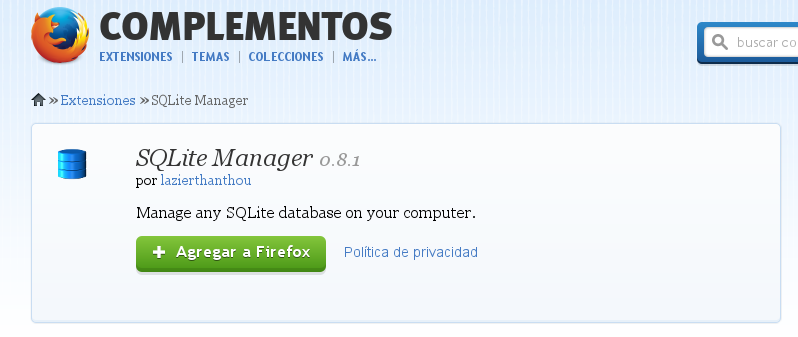
\includegraphics{sqlite_manager.png}
\begin{quote}\begin{description}
\item[{Figura 12}] \leavevmode
sqlite-manager.

\end{description}\end{quote}
\end{quote}

\end{enumerate}

\textbf{Segundo Paso:}
\begin{enumerate}
\item {} 
Abrimos \textbf{sqlite-manager} en el navegador web \textbf{Firefox}.

\item {} 
Buscamos en la barra de herramientas a \textbf{sqlite-manager}.

\item {} 
Le damos \textbf{clik} donde dice \textbf{sqlite-manager}.
\begin{quote}

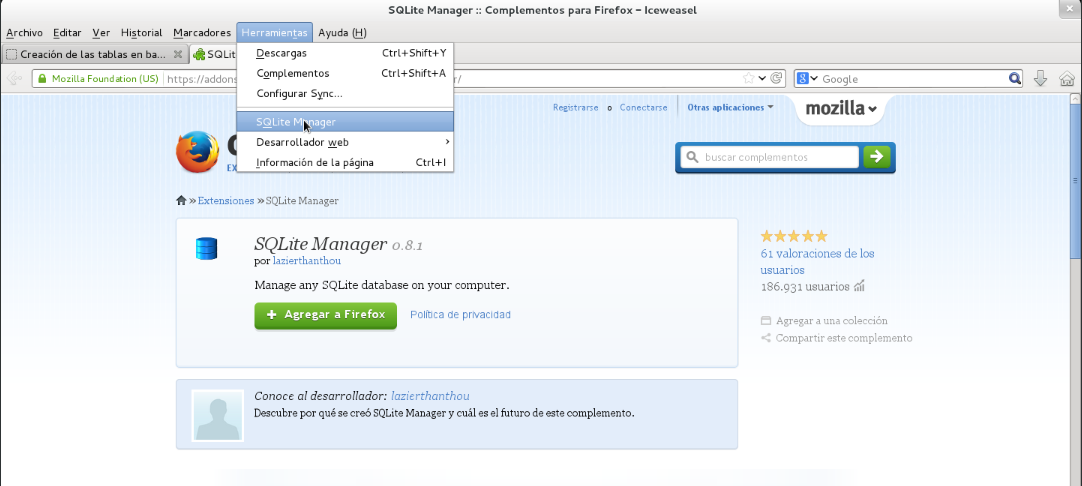
\includegraphics{buscar.png}
\begin{quote}\begin{description}
\item[{Figura 13}] \leavevmode
Navegador sqlite-manager.

\end{description}\end{quote}
\end{quote}

\item {} 
Ya tenemos la herramienta \textbf{sqlite-manager} abierta para su uso.
\begin{quote}

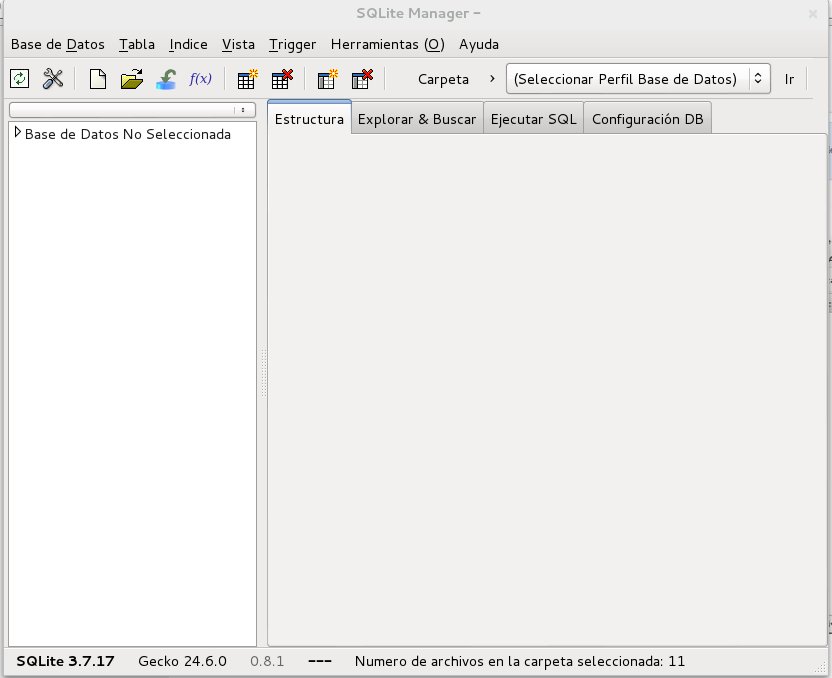
\includegraphics{buscar2.png}
\begin{quote}\begin{description}
\item[{Figura 14}] \leavevmode
sqlite-manager abierto.

\end{description}\end{quote}
\end{quote}

\end{enumerate}

\textbf{Tercer Paso:}
\begin{enumerate}
\item {} 
Creamos la base de datos.

\item {} 
Pulsamos donde esta la pagina en blanco como aparece en la imagen.
\begin{quote}

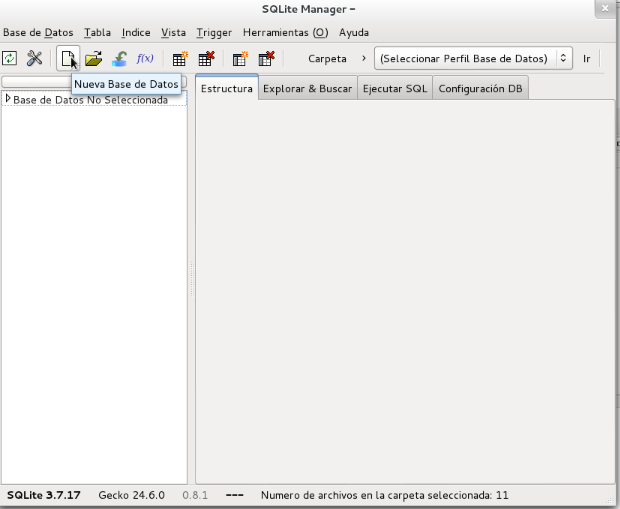
\includegraphics{buscar1.png}
\begin{quote}\begin{description}
\item[{Figura 15}] \leavevmode
Opción.

\end{description}\end{quote}
\end{quote}

\item {} 
Colocamos el nombre a la base de datos con el formato \textbf{.db}.
\begin{quote}

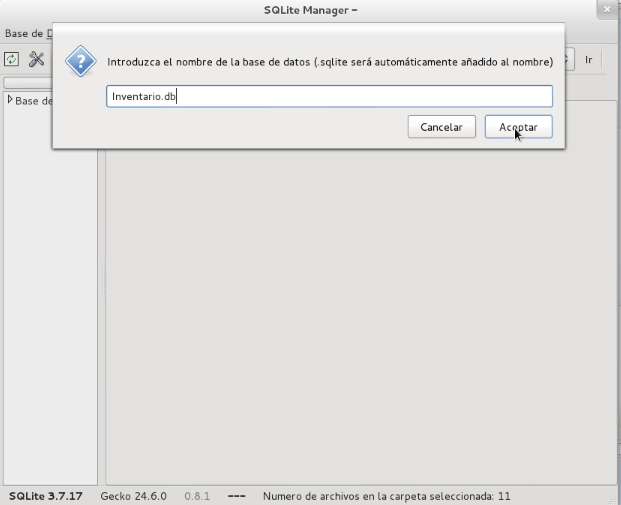
\includegraphics{basedb1.png}
\begin{quote}\begin{description}
\item[{Figura 16}] \leavevmode
Nombre de la base de datos.

\end{description}\end{quote}
\end{quote}

\item {} 
La guardamos en mi carpeta personal \textbf{\textless{}HOME\textgreater{}.safet/}.

\item {} 
Se abrirá automáticamente la base de datos con sus campos, como aparece en la siguiente imagen.
\begin{quote}

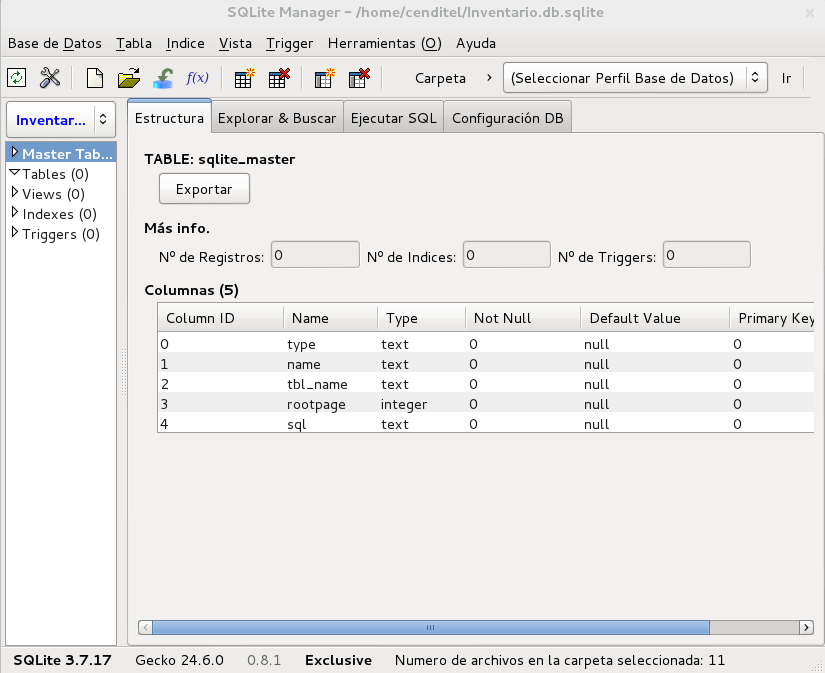
\includegraphics{buscar3.png}
\begin{quote}\begin{description}
\item[{Figura 17}] \leavevmode
Base de datos.

\end{description}\end{quote}
\end{quote}

\end{enumerate}

\textbf{Cuarto Paso:}
\begin{quote}

Creación de la tablas \textbf{``productos'', ``productos\_registro''}.
\begin{enumerate}
\item {} 
Buscamos en la barra de herramientas donde dice \textbf{Table}.

\item {} 
Pulsamos en la opción de \textbf{Crear Tabla}.
\begin{quote}

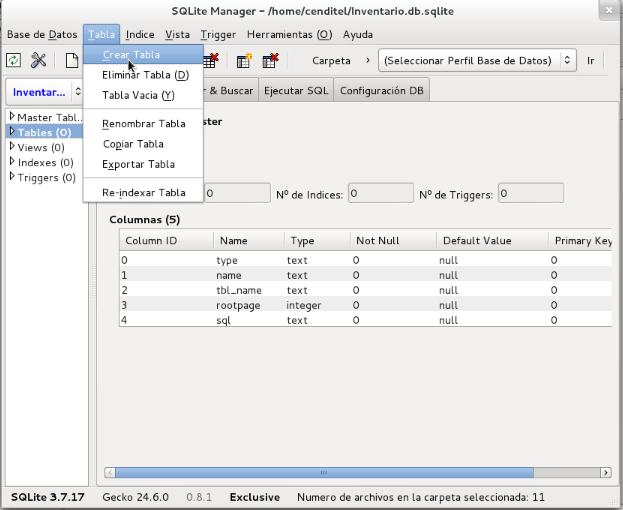
\includegraphics{tabla.png}
\begin{quote}\begin{description}
\item[{Figura 18}] \leavevmode
Opción de tables.

\end{description}\end{quote}
\end{quote}

\item {} 
Nos aparecerá un formulario vacío sin nombre ni atributos, como en la siguiente imagen.
\begin{quote}

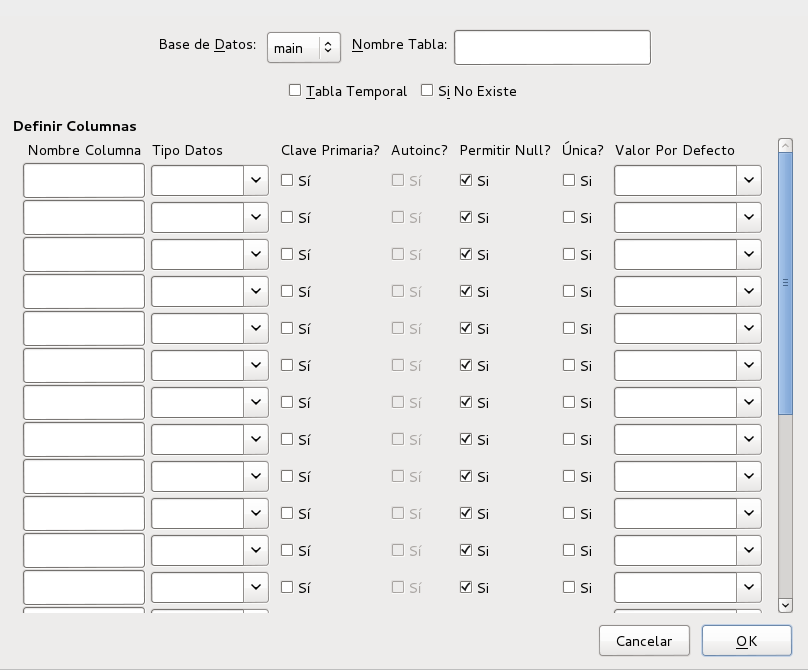
\includegraphics{tabla1.png}
\begin{quote}\begin{description}
\item[{Figura 19}] \leavevmode
Formulario de tablas.

\end{description}\end{quote}
\end{quote}

\item {} 
Llenáremos el formulario para la tabla \textbf{productos}, como aparece en la imagen.

\item {} 
Luego le pulsamos al botón \textbf{ok}.
\begin{quote}

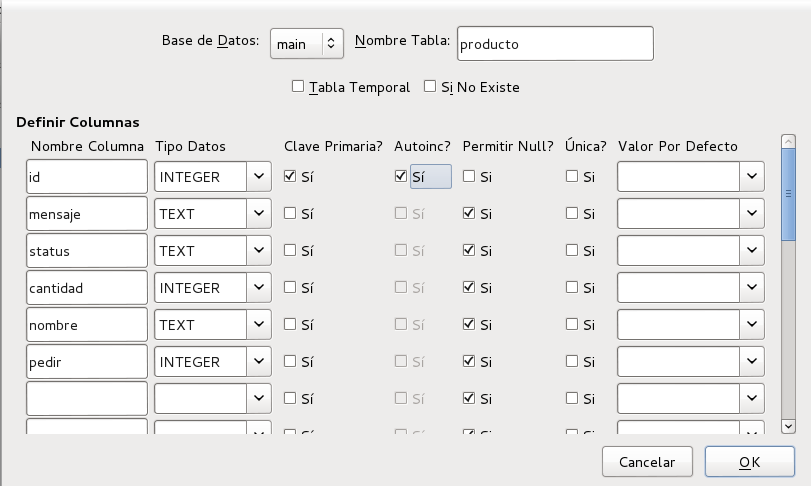
\includegraphics{tabla2.png}
\begin{quote}\begin{description}
\item[{Figura 20}] \leavevmode
Llenado del formulado de tablas.

\end{description}\end{quote}
\end{quote}

\item {} 
Nos muestra un mensaje como se muestra en la imagen.

\item {} 
Damos clik al botón \textbf{ok} para terminar con la creación.
\begin{quote}

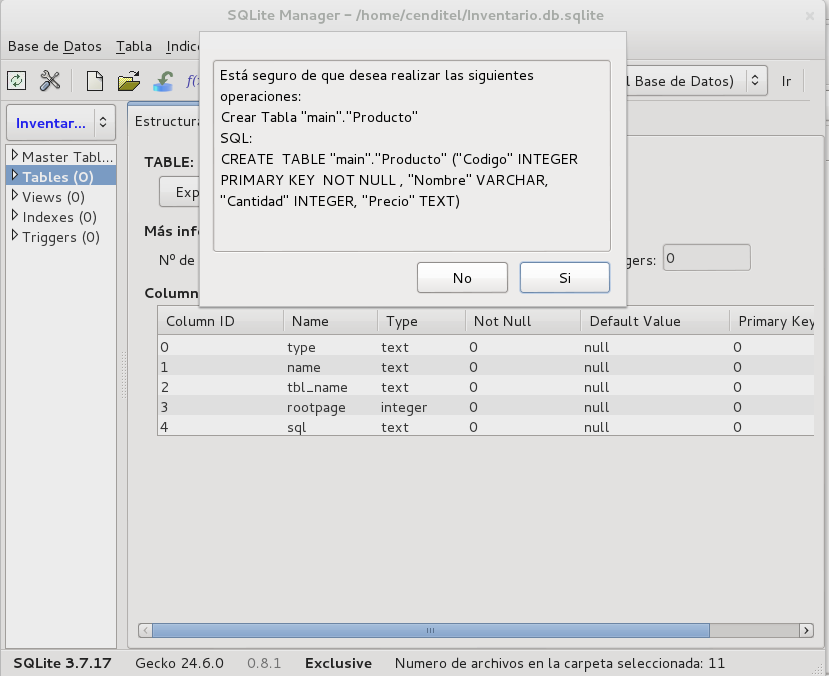
\includegraphics{tabla3.png}
\begin{quote}\begin{description}
\item[{Figura 21}] \leavevmode
Mensaje.

\end{description}\end{quote}
\end{quote}

\textbf{Nota}:

\begin{Verbatim}[commandchars=\\\{\}]
Seguimos los pasos anteriores para la creación de las demás tablas a utilizar.
\end{Verbatim}

\item {} 
Llenamos el formulario para la tabla \textbf{productos\_registro}.
\begin{quote}

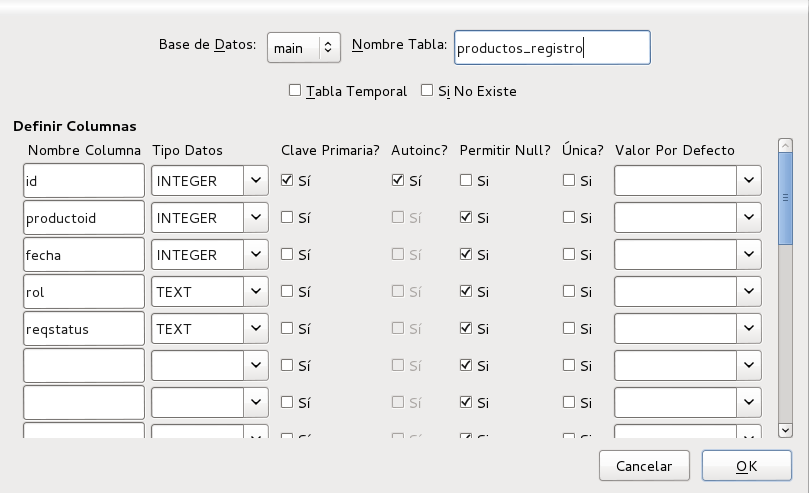
\includegraphics{tabla5.png}
\begin{quote}\begin{description}
\item[{Figura 22}] \leavevmode
Llenado del formulario de tablas.

\end{description}\end{quote}
\end{quote}

\end{enumerate}
\end{quote}

\textbf{Quinto Paso:}
\begin{enumerate}
\item {} 
Visualizamos la tabla \textbf{productos} creada.
\begin{quote}

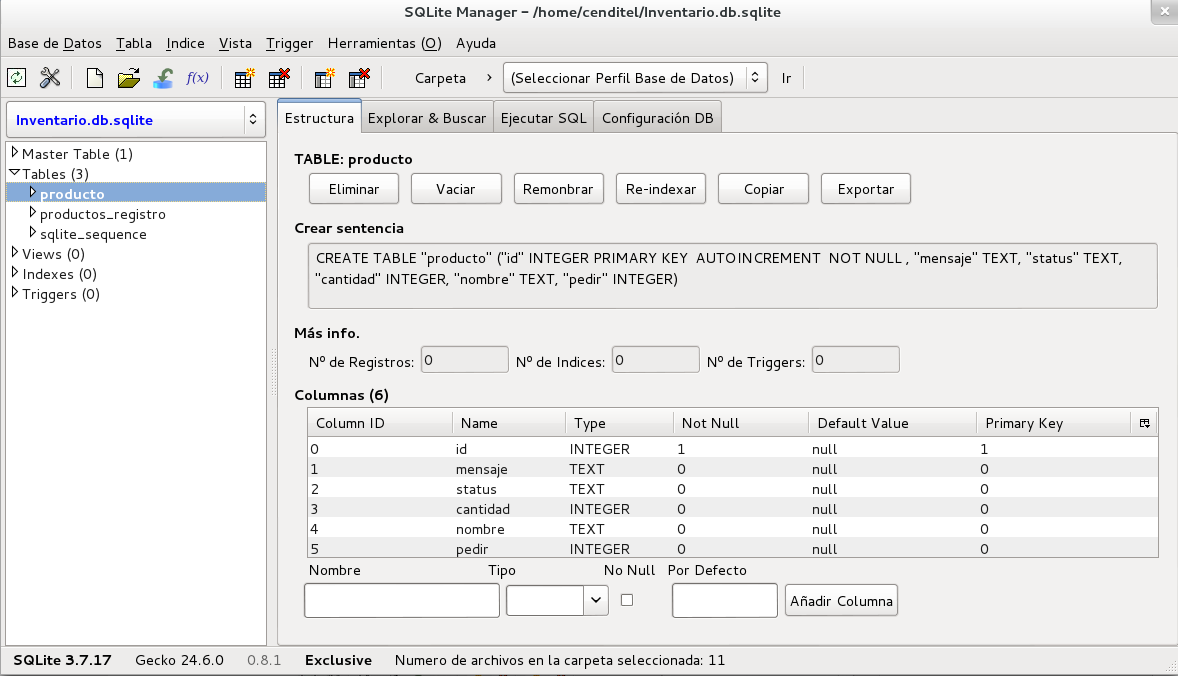
\includegraphics{producto.png}
\begin{quote}\begin{description}
\item[{Figura 23}] \leavevmode
Tabla productos.

\end{description}\end{quote}
\end{quote}

\item {} 
Visualizamos la tabla \textbf{productos\_registro} creada.
\begin{quote}

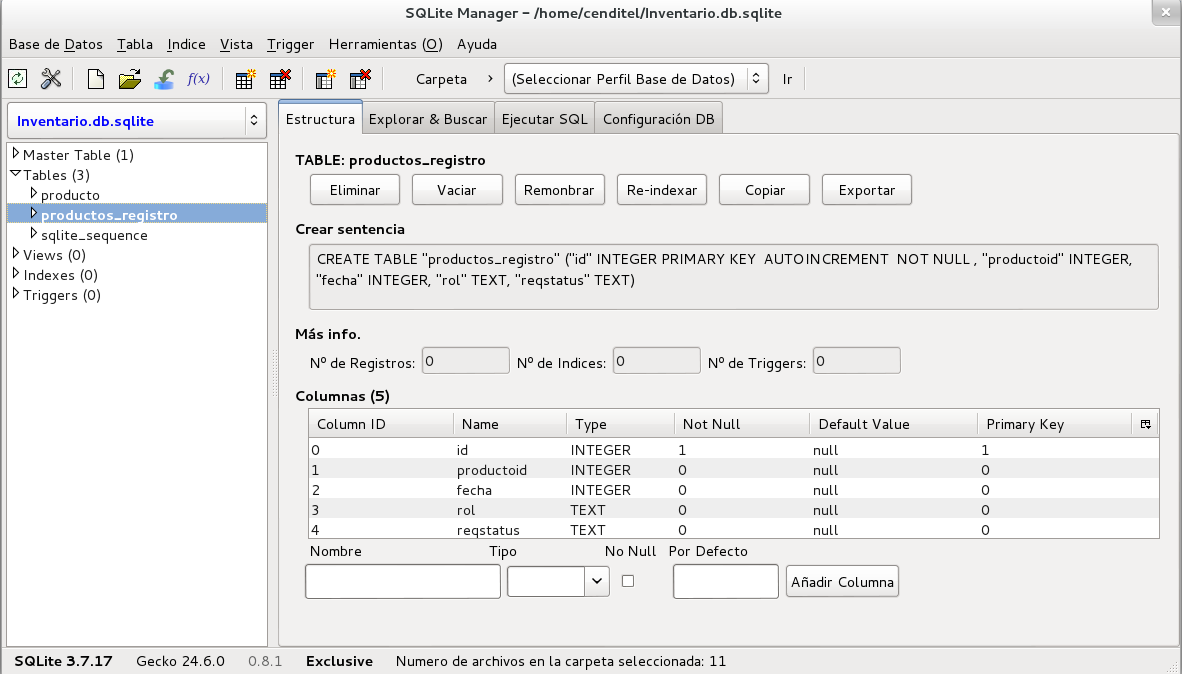
\includegraphics{producto1.png}
\begin{quote}\begin{description}
\item[{Figura 24}] \leavevmode
Tabla productos\_registro.

\end{description}\end{quote}
\end{quote}

\end{enumerate}

\textbf{¿Para qué se crean las tablas ``productos'' y ``productos\_registro''?}
\begin{itemize}
\item {} 
La tabla ``productos'' respresenta la lista de fichas \textbf{(token)} en los flujos de trabajo (Wonkflow).

\item {} 
La tabla ``productos\_registros'' representan la lasta de eventos de cambio de estado (status) en los flujos de trabajo.

\end{itemize}

\begin{Verbatim}[commandchars=\\\{\}]
\PYG{n}{NOTA}
\end{Verbatim}

Si ha seguido el tutorial correctamente obtendra los archivos que puede bajar en el enlace que se encuentran abajo
\begin{quote}

\textbf{DOWNLOAD:}


\includegraphics{download1.png}

\code{mydb.db}
\end{quote}
\end{quote}


\chapter{\index{Operaciones CRUD+(flujo) utilizando PySafet}Operaciones CRUD+(flujo) utilizando PySafet}
\label{_templates/Contenido6/Parte2:operaciones-crud-flujo-utilizando-pysafet}\label{_templates/Contenido6/Parte2::doc}
Las operaciones \href{http://es.wikipedia.org/wiki/CRUD}{CRUD}, son acciones generales que representan un modelo basíco para la creación de sistema de información. Puede ser una descripción más detallada en el siguiente enlace \href{http://www.dotnettwitter.com/2012/04/curd-operations-on-xml-file.html}{SOBRE CRUD}.

El simbolo \textbf{``+''} indica las adición de operaciones asociada a flujo de trabajo.

\textbf{A continuación comenzaremos a ver los pasos de las operaciones CRUB con un archivo que se llama deftrac.xml la cual va a estar en el directorio **\textless{}HOME\textgreater{}.safet/input/*}


\section{1° PRIMER PASO}
\label{_templates/Contenido6/Parte2:primer-paso}

\subsection{Escribimos el encabezado (información de Autor).}
\label{_templates/Contenido6/Parte2:escribimos-el-encabezado-informacion-de-autor}\begin{quote}
\begin{quote}

\begin{Verbatim}[commandchars=\\\{\}]
\PYG{c+cp}{\PYGZlt{}?xml version=\PYGZdq{}1.0\PYGZdq{} encoding=\PYGZdq{}UTF\PYGZhy{}8\PYGZdq{} ?\PYGZgt{}}
\PYG{c}{\PYGZlt{}!\PYGZhy{}\PYGZhy{}}
\PYG{c}{Documento  : deftrac.xml}
\PYG{c}{Creado     : Fulano de tal}
\PYG{c}{Autor      : Fulano de tal}
\PYG{c}{Descripcion: Archivo de Entrada para SAFET }\PYG{c}{\PYGZhy{}}\PYG{c}{ Inflow}
\PYG{c}{\PYGZhy{}\PYGZhy{}\PYGZgt{}}
\end{Verbatim}
\end{quote}
\begin{itemize}
\item {} 
\textbf{Escribimos la ruta al validador XML(formato DTD)}

\end{itemize}
\begin{quote}

\begin{Verbatim}[commandchars=\\\{\}]
\PYG{c+cp}{\PYGZlt{}!DOCTYPE operations SYSTEM \PYGZdq{}file:///home/cenditel/.safet/dtd/yawlinput.dtd\PYGZdq{}\PYGZgt{}}
\end{Verbatim}
\end{quote}
\begin{itemize}
\item {} 
\textbf{Ahora podemos empezar a escribir las operaciones siguientes:}

\end{itemize}
\begin{quote}
\begin{itemize}
\item {} 
C(Insertar)

\item {} 
R(Listar*)

\item {} 
U(Actualizar)

\item {} 
D(Borrar o eliminar)

\item {} 
+(Flujo de trabajo)

\end{itemize}

\begin{Verbatim}[commandchars=\\\{\}]
\PYG{n+nt}{\PYGZlt{}operations} \PYG{n+na}{suffix=}\PYG{l+s}{\PYGZdq{}:\PYGZdq{}} \PYG{n+na}{commandname=}\PYG{l+s}{\PYGZdq{}operacion\PYGZdq{}}\PYG{n+nt}{\PYGZgt{}}

\PYG{n+nt}{\PYGZlt{}operation}  \PYG{n+na}{name=}\PYG{l+s}{\PYGZdq{}Productos\PYGZdq{}}  \PYG{n+na}{desc=}\PYG{l+s}{\PYGZdq{}Agregar,Modificar,Eliminar,Listar\PYGZdq{}} \PYG{n+na}{icon=}\PYG{l+s}{\PYGZdq{}firmadoc.png\PYGZdq{}}\PYG{n+nt}{\PYGZgt{}} \PYG{n+nt}{\PYGZlt{}/operation\PYGZgt{}}
\end{Verbatim}
\end{quote}

\textbf{2.- Operation Insertar ``Productos'' C(Insertar)}

Las operaciones en PySafet consiste en una lista de comandos que se ejecutan secuencialmente.

Los comandos se componen de campos \textbf{``Fields''} que corresponden a los diferentes  tipos de datos básicos y complejos.  Por ejemplo analicemos el código \textbf{XML} del archivo \textbf{deftrac.xml} (operación agregar pruducto). Se define los siguiente:
\begin{quote}

\textbf{1.-} El tipo de comando es \textbf{``agregar''.(type)}, los tipos posibles son \textbf{``agregar'',''actualizar'' y ``eliminar''}.

\textbf{2.-} La tabla de la base de datos donde se realizará el comando \textbf{``command''} es \textbf{``productos''}.

\textbf{3.-} Luego se especificar la lista de campos \textbf{``fields''}. Para este campo se especificaran dos campos, el nombre del producto \textbf{``Nombre''}, y el estado del producto que tomará el valor literal \textbf{``literal'', ``Registrado''}.

\textbf{4.-} El segundo comando de la operación \textbf{``Agregar\_producto''}  también es del tipo \textbf{``Agregar''} y ojo los campos que son necesarios para registrar el eventos \textbf{``Agregar\_producto''} en la tabla \textbf{``productos\_registro''}.

\textbf{5.-} La palabra de PySafet \textbf{``\_USERNAME''} se utiliza para obtener el usuario actual
\end{quote}

A continuación se mostrara el archivo \textbf{deftrac.xml}:
\begin{quote}

\begin{Verbatim}[commandchars=\\\{\}]
\PYG{n+nt}{\PYGZlt{}operation}  \PYG{n+na}{name=}\PYG{l+s}{\PYGZdq{}agregar\PYGZus{}producto\PYGZdq{}}  \PYG{n+na}{desc=}\PYG{l+s}{\PYGZdq{}\PYGZdq{}} \PYG{n+na}{icon=}\PYG{l+s}{\PYGZdq{}plus.png\PYGZdq{}}\PYG{n+nt}{\PYGZgt{}}

\PYG{n+nt}{\PYGZlt{}command} \PYG{n+na}{id =}\PYG{l+s}{\PYGZdq{}1\PYGZdq{}} \PYG{n+na}{type=}\PYG{l+s}{\PYGZdq{}agregar\PYGZdq{}} \PYG{n+na}{table=}\PYG{l+s}{\PYGZdq{}productos\PYGZdq{}} \PYG{n+nt}{\PYGZgt{}}

 \PYG{n+nt}{\PYGZlt{}fields}\PYG{n+nt}{\PYGZgt{}}

   \PYG{n+nt}{\PYGZlt{}field} \PYG{n+na}{type=}\PYG{l+s}{\PYGZdq{}string\PYGZdq{}} \PYG{n+na}{icon=}\PYG{l+s}{\PYGZdq{}resumen.png\PYGZdq{}} \PYG{n+na}{mandatory=}\PYG{l+s}{\PYGZdq{}yes\PYGZdq{}}      \PYG{n+na}{validation=}\PYG{l+s}{\PYGZdq{}\PYGZdq{}}
                                   \PYG{n+na}{title=}\PYG{l+s}{\PYGZdq{}Nombre\PYGZdq{}} \PYG{n+na}{desc=}\PYG{l+s}{\PYGZdq{}\PYGZdq{}}\PYG{n+nt}{\PYGZgt{}}
           nombre
   \PYG{n+nt}{\PYGZlt{}/field\PYGZgt{}}

    \PYG{n+nt}{\PYGZlt{}field} \PYG{n+na}{type=}\PYG{l+s}{\PYGZdq{}string\PYGZdq{}} \PYG{n+na}{literal=}\PYG{l+s}{\PYGZdq{}Registrado\PYGZdq{}} \PYG{n+na}{mandatory=}\PYG{l+s}{\PYGZdq{}yes\PYGZdq{}} \PYG{n+nt}{\PYGZgt{}}
        status
    \PYG{n+nt}{\PYGZlt{}/field\PYGZgt{}}

 \PYG{n+nt}{\PYGZlt{}/fields\PYGZgt{}}

\PYG{n+nt}{\PYGZlt{}/command\PYGZgt{}}

\PYG{n+nt}{\PYGZlt{}command} \PYG{n+na}{id =}\PYG{l+s}{\PYGZdq{}1\PYGZdq{}} \PYG{n+na}{type=}\PYG{l+s}{\PYGZdq{}agregar\PYGZdq{}} \PYG{n+na}{table=}\PYG{l+s}{\PYGZdq{}productos\PYGZus{}registro\PYGZdq{}} \PYG{n+nt}{\PYGZgt{}}

\PYG{n+nt}{\PYGZlt{}fields}\PYG{n+nt}{\PYGZgt{}}

  \PYG{n+nt}{\PYGZlt{}field} \PYG{n+na}{type=}\PYG{l+s}{\PYGZdq{}datetime\PYGZdq{}} \PYG{n+na}{mandatory=}\PYG{l+s}{\PYGZdq{}yes\PYGZdq{}}
  \PYG{n+na}{function=}\PYG{l+s}{\PYGZdq{}seq from sqlite\PYGZus{}sequence where name=\PYGZsq{}productos\PYGZsq{}\PYGZdq{}}  \PYG{n+na}{input=}\PYG{l+s}{\PYGZdq{}no\PYGZdq{}}\PYG{n+nt}{\PYGZgt{}}
  productoid
  \PYG{n+nt}{\PYGZlt{}/field\PYGZgt{}}

  \PYG{n+nt}{\PYGZlt{}field} \PYG{n+na}{type=}\PYG{l+s}{\PYGZdq{}datetime\PYGZdq{}} \PYG{n+na}{mandatory=}\PYG{l+s}{\PYGZdq{}yes\PYGZdq{}}  \PYG{n+na}{function=}\PYG{l+s}{\PYGZdq{}datetime(\PYGZsq{}now\PYGZsq{})\PYGZdq{}}
                      \PYG{n+na}{format=}\PYG{l+s}{\PYGZdq{}time\PYGZus{}t\PYGZdq{}} \PYG{n+na}{input=}\PYG{l+s}{\PYGZdq{}no\PYGZdq{}}\PYG{n+nt}{\PYGZgt{}}
  fecha
  \PYG{n+nt}{\PYGZlt{}/field\PYGZgt{}}

  \PYG{n+nt}{\PYGZlt{}field} \PYG{n+na}{type=}\PYG{l+s}{\PYGZdq{}string\PYGZdq{}} \PYG{n+na}{literal=}\PYG{l+s}{\PYGZdq{}\PYGZus{}USERNAME\PYGZdq{}} \PYG{n+na}{mandatory=}\PYG{l+s}{\PYGZdq{}yes\PYGZdq{}} \PYG{n+nt}{\PYGZgt{}}
  rol
  \PYG{n+nt}{\PYGZlt{}/field\PYGZgt{}}

  \PYG{n+nt}{\PYGZlt{}field} \PYG{n+na}{type=}\PYG{l+s}{\PYGZdq{}string\PYGZdq{}} \PYG{n+na}{literal=}\PYG{l+s}{\PYGZdq{}Registrado\PYGZdq{}} \PYG{n+na}{mandatory=}\PYG{l+s}{\PYGZdq{}yes\PYGZdq{}} \PYG{n+nt}{\PYGZgt{}}
  regstatus
  \PYG{n+nt}{\PYGZlt{}/field\PYGZgt{}}

  \PYG{n+nt}{\PYGZlt{}/fields\PYGZgt{}}

  \PYG{n+nt}{\PYGZlt{}/command\PYGZgt{}}

  \PYG{n+nt}{\PYGZlt{}/operation\PYGZgt{}}
\end{Verbatim}
\end{quote}
\begin{itemize}
\item {} 
\textbf{Ejecutamos el Script para Insertar un producto}
\begin{quote}

Seguidamente vamos a utilizar esta operación \textbf{``agregar\_producto''} en un Script de python como se muestra a continuación:
\end{quote}

\end{itemize}
\begin{quote}
\begin{itemize}
\item {} 
\textbf{Operación:} agregar\_producto

\item {} 
\textbf{Nombre:} El nombre del Producto agregar

\end{itemize}

\begin{Verbatim}[commandchars=\\\{\}]
\PYG{c}{\PYGZsh{} \PYGZhy{}*\PYGZhy{} coding: utf\PYGZhy{}8 \PYGZhy{}*\PYGZhy{}}

\PYG{c}{\PYGZsh{} D(Borrar o eliminar)}
\PYG{c}{\PYGZsh{} myconsult = u\PYGZdq{}operacion:borrar\PYGZus{}producto id:5\PYGZdq{}}

\PYG{c}{\PYGZsh{} U(Actualizar)}
\PYG{c}{\PYGZsh{}myconsult = u\PYGZdq{}operacion:modificar\PYGZus{}producto id:3 Nombre:Amoxicilina\PYGZdq{}}

\PYG{c}{\PYGZsh{} +(Flujo de trabajo)}
\PYG{c}{\PYGZsh{} myconsult = u\PYGZdq{}operacion:Actualizar\PYGZus{}producto id:3 Estado\PYGZus{}producto:Pedido\PYGZdq{}}


\PYG{c}{\PYGZsh{} Importación de la librería Safet y os}
\PYG{k+kn}{import} \PYG{n+nn}{Safet}
\PYG{k+kn}{import} \PYG{n+nn}{os}


\PYG{c}{\PYGZsh{} Aqui obtengo mi home,media y url}
\PYG{n}{myhome} \PYG{o}{=} \PYG{n}{os}\PYG{o}{.}\PYG{n}{getenv}\PYG{p}{(}\PYG{l+s}{\PYGZdq{}}\PYG{l+s}{HOME}\PYG{l+s}{\PYGZdq{}}\PYG{p}{)}
\PYG{n}{mymedia} \PYG{o}{=} \PYG{n}{myhome} \PYG{o}{+} \PYG{l+s}{\PYGZdq{}}\PYG{l+s}{/tmp}\PYG{l+s}{\PYGZdq{}}
\PYG{n}{myurl} \PYG{o}{=} \PYG{l+s}{\PYGZdq{}}\PYG{l+s}{http://localhost}\PYG{l+s}{\PYGZdq{}}

 \PYG{c}{\PYGZsh{} Constructor principal}
\PYG{n}{myinflow} \PYG{o}{=} \PYG{n}{Safet}\PYG{o}{.}\PYG{n}{MainWindow}\PYG{p}{(}\PYG{n}{myhome}\PYG{p}{)}

\PYG{n}{myinflow}\PYG{o}{.}\PYG{n}{setMediaPath}\PYG{p}{(}\PYG{n}{mymedia}\PYG{p}{)}
\PYG{n}{myinflow}\PYG{o}{.}\PYG{n}{setHostURL}\PYG{p}{(}\PYG{n}{myurl}\PYG{p}{)}


 \PYG{c}{\PYGZsh{} Si no es un usuario registrado el metodo \PYGZdq{}login\PYGZdq{} retorna False}
\PYG{n}{result} \PYG{o}{=} \PYG{n}{myinflow}\PYG{o}{.}\PYG{n}{login}\PYG{p}{(}\PYG{l+s}{\PYGZdq{}}\PYG{l+s}{admin}\PYG{l+s}{\PYGZdq{}}\PYG{p}{,}\PYG{l+s}{\PYGZdq{}}\PYG{l+s}{admin}\PYG{l+s}{\PYGZdq{}}\PYG{p}{)}

\PYG{c}{\PYGZsh{} C(Insertar)}
\PYG{c}{\PYGZsh{} Agregamos el poducto a ingresar por ejemplo \PYGZdq{}Champu Olorin\PYGZdq{},}
\PYG{c}{\PYGZsh{}                    \PYGZdq{}ComplejoB\PYGZdq{},\PYGZdq{}Aspirina\PYGZdq{},\PYGZdq{}Acetaminofén\PYGZdq{},\PYGZdq{}Ibuprofeno\PYGZdq{}.}

\PYG{n}{myconsult} \PYG{o}{=} \PYG{l+s}{u\PYGZdq{}}\PYG{l+s}{operacion:agregar\PYGZus{}producto  Nombre: ComplejoB}\PYG{l+s}{\PYGZdq{}}

\PYG{k}{if} \PYG{n}{result}\PYG{p}{:}
        \PYG{n}{result} \PYG{o}{=} \PYG{n}{myinflow}\PYG{o}{.}\PYG{n}{toInputForm}\PYG{p}{(}\PYG{n}{myconsult}\PYG{p}{)}
\PYG{k}{else}\PYG{p}{:}
        \PYG{k}{print} \PYG{l+s}{\PYGZdq{}}\PYG{l+s+se}{\PYGZbs{}n}\PYG{l+s}{ \PYGZhy{}\PYGZhy{}\PYGZhy{}Usuario autenticado\PYGZhy{}\PYGZhy{}\PYGZhy{}}\PYG{l+s+se}{\PYGZbs{}n}\PYG{l+s}{\PYGZdq{}}
        \PYG{n+nb}{exit}\PYG{p}{(}\PYG{p}{)}


\PYG{k}{if} \PYG{n}{result}\PYG{p}{:}
        \PYG{k}{print} \PYG{l+s}{\PYGZdq{}}\PYG{l+s+se}{\PYGZbs{}n}\PYG{l+s}{ \PYGZhy{}\PYGZhy{}Se Actualizo correctamente el producto\PYGZhy{}\PYGZhy{}\PYGZhy{}}\PYG{l+s+se}{\PYGZbs{}n}\PYG{l+s}{\PYGZdq{}}
\PYG{k}{else}\PYG{p}{:}
        \PYG{k}{print} \PYG{l+s}{\PYGZdq{}}\PYG{l+s+se}{\PYGZbs{}n}\PYG{l+s}{ No se Actualizo el producto....!!!}\PYG{l+s+se}{\PYGZbs{}n}\PYG{l+s}{\PYGZdq{}}


\PYG{k}{if} \PYG{o+ow}{not} \PYG{n}{result}\PYG{p}{:}
        \PYG{k}{print} \PYG{l+s}{\PYGZdq{}}\PYG{l+s+se}{\PYGZbs{}n}\PYG{l+s}{Consulta failed error: }\PYG{l+s+si}{\PYGZpc{}s}\PYG{l+s+se}{\PYGZbs{}n}\PYG{l+s}{\PYGZdq{}} \PYG{o}{\PYGZpc{}} \PYG{p}{(}\PYG{n}{myinflow}\PYG{o}{.}\PYG{n}{currentError}\PYG{p}{(}\PYG{p}{)}\PYG{p}{)}
        \PYG{n+nb}{exit}\PYG{p}{(}\PYG{p}{)}

\PYG{k}{print} \PYG{l+s}{u\PYGZdq{}}\PYG{l+s}{  }\PYG{l+s+si}{\PYGZpc{}s}\PYG{l+s+se}{\PYGZbs{}n}\PYG{l+s}{\PYGZdq{}} \PYG{o}{\PYGZpc{}} \PYG{p}{(}\PYG{n}{myinflow}\PYG{o}{.}\PYG{n}{currentJSON}\PYG{p}{(}\PYG{p}{)}\PYG{p}{)}
\end{Verbatim}
\end{quote}
\begin{description}
\item[{Crearemos un archivo \textbf{''.py''} con cualquier nombre y copiamos el \textbf{Script} y lo ejecutamos de la siguiente manera:}] \leavevmode
\begin{Verbatim}[commandchars=\\\{\}]
\PYGZdl{} python Script\PYGZus{}Insertar\PYGZus{}producto.py
\end{Verbatim}

\end{description}
\begin{itemize}
\item {} 
\textbf{Observen la siguiente imagen:}
\begin{quote}

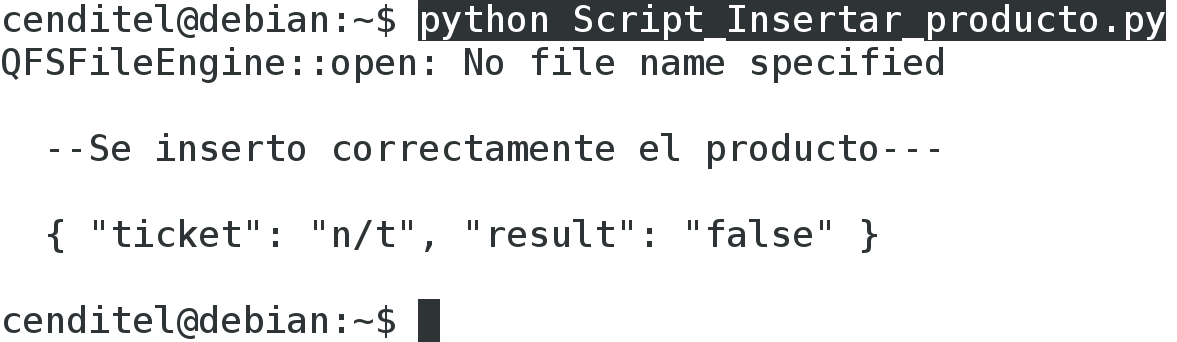
\includegraphics{insertar1.png}
\begin{quote}\begin{description}
\item[{Figura 25}] \leavevmode
Insertar producto.

\end{description}\end{quote}
\end{quote}

\item {} 
\textbf{Observen la base de datos en la siguiente imagen:}
\begin{quote}
\begin{figure}[htbp]
\centering
\capstart

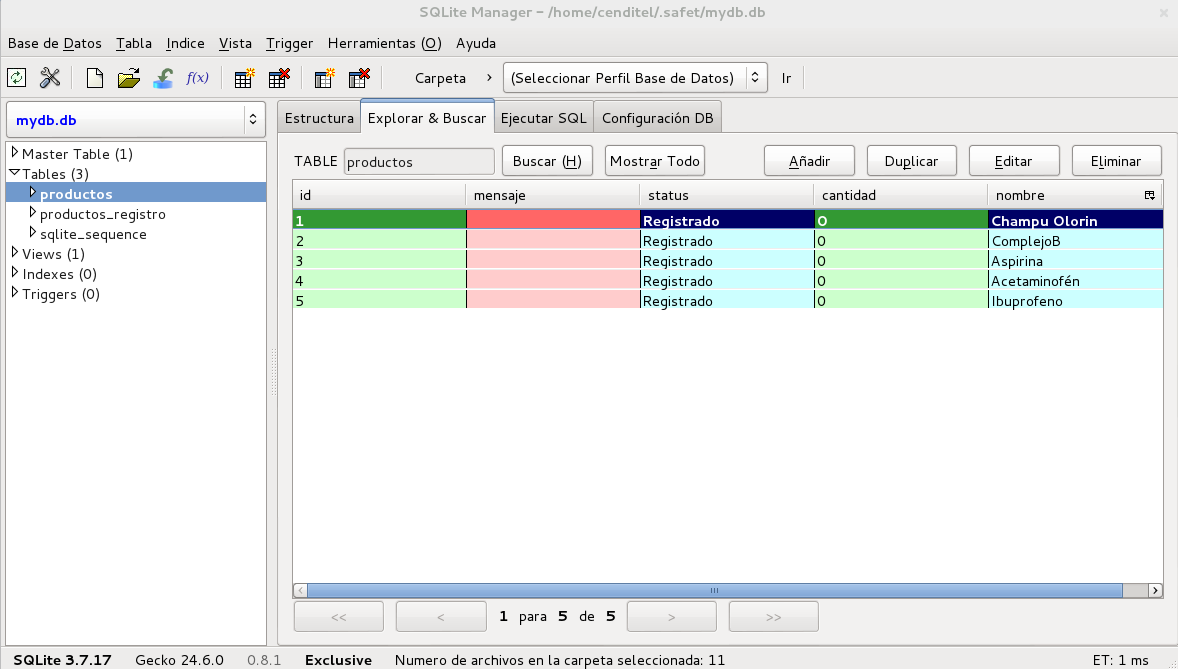
\includegraphics{lista_producto3.png}
\caption{\textbf{Figura 26: Tabla productos}}\label{_templates/Contenido6/Parte2:figura1}\end{figure}
\end{quote}

{\hfill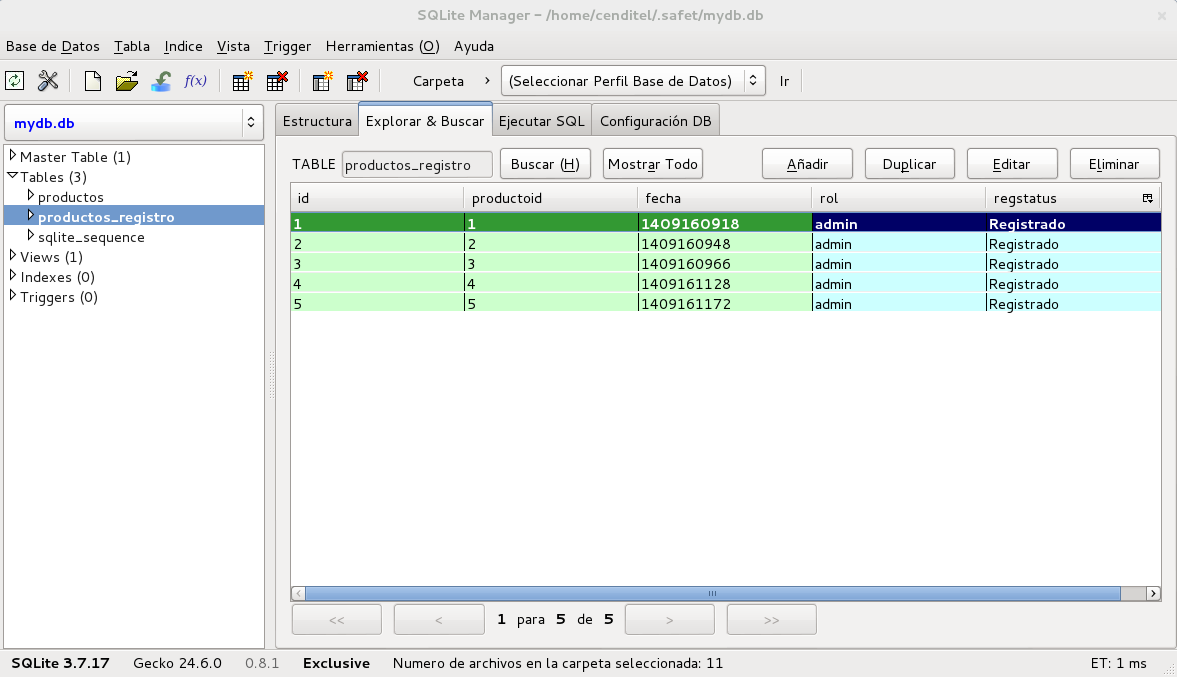
\includegraphics{lista_producto4.png}\hfill}
\begin{quote}\begin{description}
\item[{Figura 27}] \leavevmode
Tabla productos\_registro.

\end{description}\end{quote}

\end{itemize}

\textbf{3.- Operation Eliminar ``Productos'' D(Borrar o eliminar)}
\begin{quote}

\begin{Verbatim}[commandchars=\\\{\}]
\PYGZlt{}operation  name=\PYGZdq{}borrar\PYGZus{}producto\PYGZdq{}  desc=\PYGZdq{}Elimina un ticket por id\PYGZdq{} icon=\PYGZdq{}clear.png\PYGZdq{}\PYGZgt{}

        \PYGZlt{}command id =\PYGZdq{}1\PYGZdq{} type=\PYGZdq{}eliminar\PYGZdq{} table=\PYGZdq{}productos\PYGZdq{}\PYGZgt{}

                \PYGZlt{}fields\PYGZgt{}

                        \PYGZlt{}field type=\PYGZdq{}combolisttable\PYGZdq{} options=\PYGZdq{}id:productos::id \textbar{}\textbar{} \PYGZsq{} \PYGZhy{} \PYGZsq{} \textbar{}\textbar{} nombre\PYGZdq{}
                                                                mandatory=\PYGZdq{}yes\PYGZdq{} primarykey=\PYGZdq{}yes\PYGZdq{} title=\PYGZdq{}id\PYGZdq{} \PYGZgt{}
                        id
                        \PYGZlt{}/field\PYGZgt{}

                \PYGZlt{}/fields\PYGZgt{}

        \PYGZlt{}/command\PYGZgt{}

        \PYGZlt{}command id =\PYGZdq{}1\PYGZdq{} type=\PYGZdq{}eliminar\PYGZdq{} table=\PYGZdq{}productos\PYGZus{}registro\PYGZdq{}\PYGZgt{}

                \PYGZlt{}fields\PYGZgt{}

                        \PYGZlt{}field type=\PYGZdq{}string\PYGZdq{}  mandatory=\PYGZdq{}yes\PYGZdq{} title=\PYGZdq{}id\PYGZdq{} \PYGZgt{}
                        productoid
                        \PYGZlt{}/field\PYGZgt{}

                \PYGZlt{}/fields\PYGZgt{}

        \PYGZlt{}/command\PYGZgt{}

\PYGZlt{}/operation\PYGZgt{}
\end{Verbatim}
\end{quote}
\begin{itemize}
\item {} 
\textbf{Ejecutamos el Script para elimiar el producto}
\begin{quote}

Seguidamente vamos a utilizar esta operación \textbf{``borrar\_producto''} en un Script de python como se muestra a continuación:
\end{quote}

\end{itemize}
\begin{quote}
\begin{itemize}
\item {} 
\textbf{Operación:} borrar\_producto

\item {} 
\textbf{id:} Aqui colocaremos el valor de \textbf{id} del producto por ejemplo borraremos el producto \textbf{Ibuprofeno} y su \textbf{id} es \textbf{5}. Observe la {\hyperref[_templates/Contenido6/Parte2:figura1]{\emph{Figura 26: Tabla productos}}}

\end{itemize}

\begin{Verbatim}[commandchars=\\\{\}]
\PYG{c}{\PYGZsh{} \PYGZhy{}*\PYGZhy{} coding: utf\PYGZhy{}8 \PYGZhy{}*\PYGZhy{}}

\PYG{c}{\PYGZsh{} C(Insertar)}
\PYG{c}{\PYGZsh{} Agregamos el poducto a ingresar por ejemplo \PYGZdq{}Champu Olorin\PYGZdq{},}
\PYG{c}{\PYGZsh{}                    \PYGZdq{}ComplejoB\PYGZdq{},\PYGZdq{}Aspirina\PYGZdq{},\PYGZdq{}Acetaminofén\PYGZdq{},\PYGZdq{}Ibuprofeno\PYGZdq{}.}
\PYG{c}{\PYGZsh{}myconsult = u\PYGZdq{}operacion:agregar\PYGZus{}producto  Nombre: ComplejoB\PYGZdq{}}

\PYG{c}{\PYGZsh{} U(Actualizar)}
\PYG{c}{\PYGZsh{}myconsult = u\PYGZdq{}operacion:modificar\PYGZus{}producto id:3 Nombre:Amoxicilina\PYGZdq{}}

\PYG{c}{\PYGZsh{} +(Flujo de trabajo)}
\PYG{c}{\PYGZsh{} myconsult = u\PYGZdq{}operacion:Actualizar\PYGZus{}producto id:3 Estado\PYGZus{}producto:Pedido\PYGZdq{}}


\PYG{c}{\PYGZsh{} Importación de la librería Safet y os}
\PYG{k+kn}{import} \PYG{n+nn}{Safet}
\PYG{k+kn}{import} \PYG{n+nn}{os}


\PYG{c}{\PYGZsh{} Aqui obtengo mi home,media y url}
\PYG{n}{myhome} \PYG{o}{=} \PYG{n}{os}\PYG{o}{.}\PYG{n}{getenv}\PYG{p}{(}\PYG{l+s}{\PYGZdq{}}\PYG{l+s}{HOME}\PYG{l+s}{\PYGZdq{}}\PYG{p}{)}
\PYG{n}{mymedia} \PYG{o}{=} \PYG{n}{myhome} \PYG{o}{+} \PYG{l+s}{\PYGZdq{}}\PYG{l+s}{/tmp}\PYG{l+s}{\PYGZdq{}}
\PYG{n}{myurl} \PYG{o}{=} \PYG{l+s}{\PYGZdq{}}\PYG{l+s}{http://localhost}\PYG{l+s}{\PYGZdq{}}

 \PYG{c}{\PYGZsh{} Constructor principal}
\PYG{n}{myinflow} \PYG{o}{=} \PYG{n}{Safet}\PYG{o}{.}\PYG{n}{MainWindow}\PYG{p}{(}\PYG{n}{myhome}\PYG{p}{)}

\PYG{n}{myinflow}\PYG{o}{.}\PYG{n}{setMediaPath}\PYG{p}{(}\PYG{n}{mymedia}\PYG{p}{)}
\PYG{n}{myinflow}\PYG{o}{.}\PYG{n}{setHostURL}\PYG{p}{(}\PYG{n}{myurl}\PYG{p}{)}


 \PYG{c}{\PYGZsh{} Si no es un usuario registrado el metodo \PYGZdq{}login\PYGZdq{} retorna False}
\PYG{n}{result} \PYG{o}{=} \PYG{n}{myinflow}\PYG{o}{.}\PYG{n}{login}\PYG{p}{(}\PYG{l+s}{\PYGZdq{}}\PYG{l+s}{admin}\PYG{l+s}{\PYGZdq{}}\PYG{p}{,}\PYG{l+s}{\PYGZdq{}}\PYG{l+s}{admin}\PYG{l+s}{\PYGZdq{}}\PYG{p}{)}

\PYG{c}{\PYGZsh{} D(Borrar o eliminar)}
\PYG{c}{\PYGZsh{} Eliminamos el porducto numero 5}
\PYG{n}{myconsult} \PYG{o}{=} \PYG{l+s}{u\PYGZdq{}}\PYG{l+s}{operacion:borrar\PYGZus{}producto id:5}\PYG{l+s}{\PYGZdq{}}

\PYG{k}{if} \PYG{n}{result}\PYG{p}{:}
        \PYG{n}{result} \PYG{o}{=} \PYG{n}{myinflow}\PYG{o}{.}\PYG{n}{toInputForm}\PYG{p}{(}\PYG{n}{myconsult}\PYG{p}{)}
\PYG{k}{else}\PYG{p}{:}
        \PYG{k}{print} \PYG{l+s}{\PYGZdq{}}\PYG{l+s+se}{\PYGZbs{}n}\PYG{l+s}{ \PYGZhy{}\PYGZhy{}\PYGZhy{}Usuario autenticado\PYGZhy{}\PYGZhy{}\PYGZhy{}}\PYG{l+s+se}{\PYGZbs{}n}\PYG{l+s}{\PYGZdq{}}
        \PYG{n+nb}{exit}\PYG{p}{(}\PYG{p}{)}


\PYG{k}{if} \PYG{n}{result}\PYG{p}{:}
        \PYG{k}{print} \PYG{l+s}{\PYGZdq{}}\PYG{l+s+se}{\PYGZbs{}n}\PYG{l+s}{ \PYGZhy{}\PYGZhy{}Se Actualizo correctamente el producto\PYGZhy{}\PYGZhy{}\PYGZhy{}}\PYG{l+s+se}{\PYGZbs{}n}\PYG{l+s}{\PYGZdq{}}
\PYG{k}{else}\PYG{p}{:}
        \PYG{k}{print} \PYG{l+s}{\PYGZdq{}}\PYG{l+s+se}{\PYGZbs{}n}\PYG{l+s}{ No se Actualizo el producto....!!!}\PYG{l+s+se}{\PYGZbs{}n}\PYG{l+s}{\PYGZdq{}}


\PYG{k}{if} \PYG{o+ow}{not} \PYG{n}{result}\PYG{p}{:}
        \PYG{k}{print} \PYG{l+s}{\PYGZdq{}}\PYG{l+s+se}{\PYGZbs{}n}\PYG{l+s}{Consulta failed error: }\PYG{l+s+si}{\PYGZpc{}s}\PYG{l+s+se}{\PYGZbs{}n}\PYG{l+s}{\PYGZdq{}} \PYG{o}{\PYGZpc{}} \PYG{p}{(}\PYG{n}{myinflow}\PYG{o}{.}\PYG{n}{currentError}\PYG{p}{(}\PYG{p}{)}\PYG{p}{)}
        \PYG{n+nb}{exit}\PYG{p}{(}\PYG{p}{)}

\PYG{k}{print} \PYG{l+s}{u\PYGZdq{}}\PYG{l+s}{  }\PYG{l+s+si}{\PYGZpc{}s}\PYG{l+s+se}{\PYGZbs{}n}\PYG{l+s}{\PYGZdq{}} \PYG{o}{\PYGZpc{}} \PYG{p}{(}\PYG{n}{myinflow}\PYG{o}{.}\PYG{n}{currentJSON}\PYG{p}{(}\PYG{p}{)}\PYG{p}{)}
\end{Verbatim}

\begin{Verbatim}[commandchars=\\\{\}]
\PYG{n+nv}{\PYGZdl{} }python Eliminar\PYGZus{}producto.py
\end{Verbatim}
\end{quote}

\textbf{Observen la siguiente imagen:}
\begin{quote}

{\hfill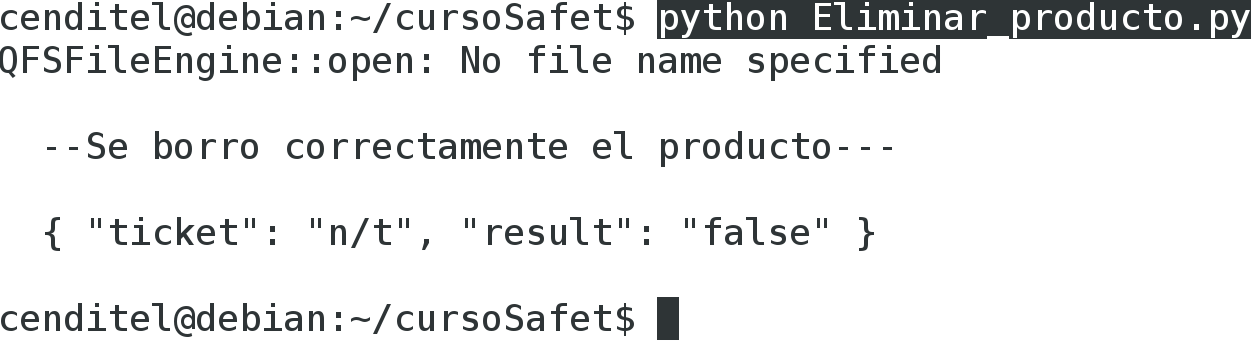
\includegraphics{Eliminar.png}\hfill}
\begin{quote}\begin{description}
\item[{Figura 27}] \leavevmode
Script Eliminar producto.

\end{description}\end{quote}
\end{quote}
\begin{itemize}
\item {} 
\textbf{Observen en la db en la siguiente imagen:} Observe la {\hyperref[_templates/Contenido6/Parte2:figura2]{\emph{Figura 26: Tabla productos}}}
\begin{quote}
\begin{figure}[htbp]
\centering
\capstart

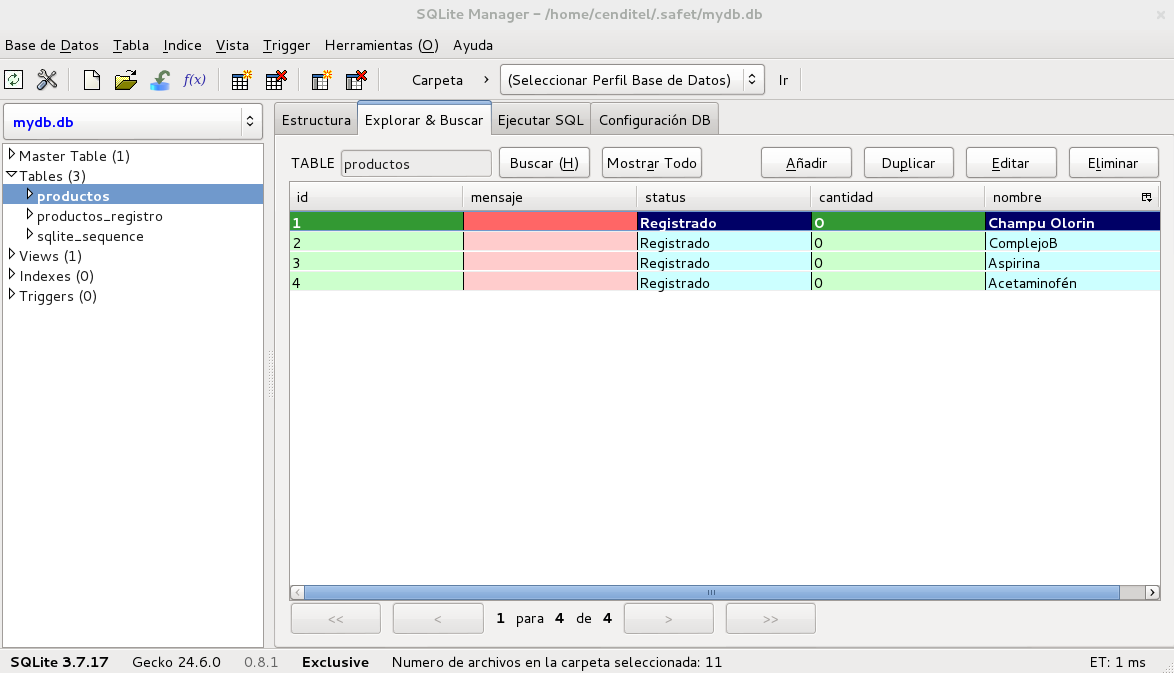
\includegraphics{Eliminar1.png}
\caption{\textbf{Figura 26: Tabla productos}}\label{_templates/Contenido6/Parte2:figura2}\end{figure}
\end{quote}

\item {} 
\textbf{Observen en la db en la siguiente imagen:} Observe la {\hyperref[_templates/Contenido6/Parte2:figura3]{\emph{Figura 27: Tabla productos\_registro}}}
\begin{quote}
\begin{figure}[htbp]
\centering
\capstart

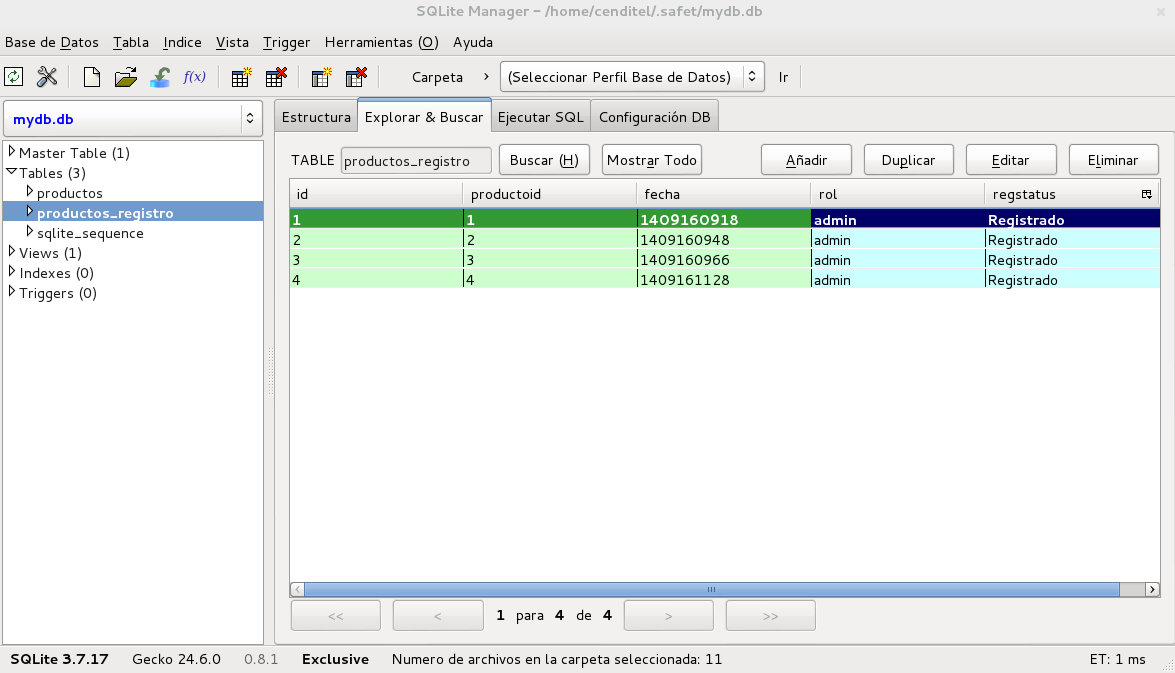
\includegraphics{Eliminar2.png}
\caption{\textbf{Figura 27: Tabla productos\_registro}}\label{_templates/Contenido6/Parte2:figura3}\end{figure}
\end{quote}

\end{itemize}
\end{quote}

\textbf{4.- Operation Actualizar ``Nombre del Producto'' U(Actualizar)}
\begin{quote}
\begin{quote}

\begin{Verbatim}[commandchars=\\\{\}]
\PYGZlt{}operation  name=\PYGZdq{}modificar\PYGZus{}producto\PYGZdq{}  desc=\PYGZdq{}\PYGZdq{} icon=\PYGZdq{}plus.png\PYGZdq{}\PYGZgt{}

        \PYGZlt{}command id =\PYGZdq{}1\PYGZdq{} type=\PYGZdq{}actualizar\PYGZdq{} table=\PYGZdq{}productos\PYGZdq{} \PYGZgt{}

                \PYGZlt{}fields\PYGZgt{}

                        \PYGZlt{}field type=\PYGZdq{}combolisttable\PYGZdq{} options=\PYGZdq{}id:productos::id \textbar{}\textbar{} \PYGZsq{} \PYGZhy{} \PYGZsq{} \textbar{}\textbar{} nombre\PYGZdq{}
                                                mandatory=\PYGZdq{}yes\PYGZdq{} primarykey=\PYGZdq{}yes\PYGZdq{} title=\PYGZdq{}id\PYGZdq{} order=\PYGZdq{}desc\PYGZdq{}\PYGZgt{}
                        id
                        \PYGZlt{}/field\PYGZgt{}

                        \PYGZlt{}field type=\PYGZdq{}string\PYGZdq{} icon=\PYGZdq{}resumen.png\PYGZdq{} mandatory=\PYGZdq{}yes\PYGZdq{} validation=\PYGZdq{}\PYGZdq{}
                                                                title=\PYGZdq{}Nombre\PYGZdq{} desc=\PYGZdq{}\PYGZdq{}\PYGZgt{}
                        nombre
                        \PYGZlt{}/field\PYGZgt{}

                \PYGZlt{}/fields\PYGZgt{}

        \PYGZlt{}/command\PYGZgt{}

\PYGZlt{}/operation\PYGZgt{}
\end{Verbatim}
\end{quote}
\begin{itemize}
\item {} 
\textbf{Ejecutamos el Script para Actualizar el nombre producto}
\begin{quote}

Seguidamente vamos a utilizar esta operación \textbf{``Actualizar\_producto''} en un Script de python como se muestra a continuación:
\end{quote}

\end{itemize}
\begin{quote}
\begin{itemize}
\item {} 
\textbf{Operación:} modificar\_producto

\item {} 
\textbf{id:} Aqui colocaremos el valor de \textbf{id} del producto por ejemplo vamos a actualizar el producto \textbf{Aspirina} y su \textbf{id} es \textbf{3}. Observe la {\hyperref[_templates/Contenido6/Parte2:figura1]{\emph{Figura 26: Tabla productos}}}

\item {} 
\textbf{Nombre:} Aqui se coloca el nombre al que le vamos a modificar por ejemplo \textbf{Amoxacilina} por \textbf{Aspirina}.

\end{itemize}

\begin{Verbatim}[commandchars=\\\{\}]
\PYG{c}{\PYGZsh{} \PYGZhy{}*\PYGZhy{} coding: utf\PYGZhy{}8 \PYGZhy{}*\PYGZhy{}}

\PYG{c}{\PYGZsh{} C(Insertar)}
\PYG{c}{\PYGZsh{} Agregamos el poducto a ingresar por ejemplo \PYGZdq{}Champu Olorin\PYGZdq{},}
\PYG{c}{\PYGZsh{}                    \PYGZdq{}ComplejoB\PYGZdq{},\PYGZdq{}Aspirina\PYGZdq{},\PYGZdq{}Acetaminofén\PYGZdq{},\PYGZdq{}Ibuprofeno\PYGZdq{}.}
\PYG{c}{\PYGZsh{}myconsult = u\PYGZdq{}operacion:agregar\PYGZus{}producto  Nombre: ComplejoB\PYGZdq{}}

\PYG{c}{\PYGZsh{} D(Borrar o eliminar)}
\PYG{c}{\PYGZsh{} Eliminamos el porducto numero 5}
\PYG{c}{\PYGZsh{}myconsult = u\PYGZdq{}operacion:borrar\PYGZus{}producto id:5\PYGZdq{}}


\PYG{c}{\PYGZsh{} +(Flujo de trabajo)}
\PYG{c}{\PYGZsh{} myconsult = u\PYGZdq{}operacion:Actualizar\PYGZus{}producto id:3 Estado\PYGZus{}producto:Pedido\PYGZdq{}}


\PYG{c}{\PYGZsh{} Importación de la librería Safet y os}
\PYG{k+kn}{import} \PYG{n+nn}{Safet}
\PYG{k+kn}{import} \PYG{n+nn}{os}


\PYG{c}{\PYGZsh{} Aqui obtengo mi home,media y url}
\PYG{n}{myhome} \PYG{o}{=} \PYG{n}{os}\PYG{o}{.}\PYG{n}{getenv}\PYG{p}{(}\PYG{l+s}{\PYGZdq{}}\PYG{l+s}{HOME}\PYG{l+s}{\PYGZdq{}}\PYG{p}{)}
\PYG{n}{mymedia} \PYG{o}{=} \PYG{n}{myhome} \PYG{o}{+} \PYG{l+s}{\PYGZdq{}}\PYG{l+s}{/tmp}\PYG{l+s}{\PYGZdq{}}
\PYG{n}{myurl} \PYG{o}{=} \PYG{l+s}{\PYGZdq{}}\PYG{l+s}{http://localhost}\PYG{l+s}{\PYGZdq{}}

 \PYG{c}{\PYGZsh{} Constructor principal}
\PYG{n}{myinflow} \PYG{o}{=} \PYG{n}{Safet}\PYG{o}{.}\PYG{n}{MainWindow}\PYG{p}{(}\PYG{n}{myhome}\PYG{p}{)}

\PYG{n}{myinflow}\PYG{o}{.}\PYG{n}{setMediaPath}\PYG{p}{(}\PYG{n}{mymedia}\PYG{p}{)}
\PYG{n}{myinflow}\PYG{o}{.}\PYG{n}{setHostURL}\PYG{p}{(}\PYG{n}{myurl}\PYG{p}{)}


\PYG{c}{\PYGZsh{} Si no es un usuario registrado el metodo \PYGZdq{}login\PYGZdq{} retorna False}
\PYG{n}{result} \PYG{o}{=} \PYG{n}{myinflow}\PYG{o}{.}\PYG{n}{login}\PYG{p}{(}\PYG{l+s}{\PYGZdq{}}\PYG{l+s}{admin}\PYG{l+s}{\PYGZdq{}}\PYG{p}{,}\PYG{l+s}{\PYGZdq{}}\PYG{l+s}{admin}\PYG{l+s}{\PYGZdq{}}\PYG{p}{)}

\PYG{c}{\PYGZsh{} U(Actualizar)}
\PYG{c}{\PYGZsh{} Se actualizara el nombre del producto número 3}
\PYG{n}{myconsult} \PYG{o}{=} \PYG{l+s}{u\PYGZdq{}}\PYG{l+s}{operacion:modificar\PYGZus{}producto id:3 Nombre:Amoxicilina}\PYG{l+s}{\PYGZdq{}}

\PYG{k}{if} \PYG{n}{result}\PYG{p}{:}
        \PYG{n}{result} \PYG{o}{=} \PYG{n}{myinflow}\PYG{o}{.}\PYG{n}{toInputForm}\PYG{p}{(}\PYG{n}{myconsult}\PYG{p}{)}
\PYG{k}{else}\PYG{p}{:}
        \PYG{k}{print} \PYG{l+s}{\PYGZdq{}}\PYG{l+s+se}{\PYGZbs{}n}\PYG{l+s}{ \PYGZhy{}\PYGZhy{}\PYGZhy{}Usuario autenticado\PYGZhy{}\PYGZhy{}\PYGZhy{}}\PYG{l+s+se}{\PYGZbs{}n}\PYG{l+s}{\PYGZdq{}}
        \PYG{n+nb}{exit}\PYG{p}{(}\PYG{p}{)}


\PYG{k}{if} \PYG{n}{result}\PYG{p}{:}
        \PYG{k}{print} \PYG{l+s}{\PYGZdq{}}\PYG{l+s+se}{\PYGZbs{}n}\PYG{l+s}{ \PYGZhy{}\PYGZhy{}Se Actualizo correctamente el producto\PYGZhy{}\PYGZhy{}\PYGZhy{}}\PYG{l+s+se}{\PYGZbs{}n}\PYG{l+s}{\PYGZdq{}}
\PYG{k}{else}\PYG{p}{:}
        \PYG{k}{print} \PYG{l+s}{\PYGZdq{}}\PYG{l+s+se}{\PYGZbs{}n}\PYG{l+s}{ No se Actualizo el producto....!!!}\PYG{l+s+se}{\PYGZbs{}n}\PYG{l+s}{\PYGZdq{}}


\PYG{k}{if} \PYG{o+ow}{not} \PYG{n}{result}\PYG{p}{:}
        \PYG{k}{print} \PYG{l+s}{\PYGZdq{}}\PYG{l+s+se}{\PYGZbs{}n}\PYG{l+s}{Consulta failed error: }\PYG{l+s+si}{\PYGZpc{}s}\PYG{l+s+se}{\PYGZbs{}n}\PYG{l+s}{\PYGZdq{}} \PYG{o}{\PYGZpc{}} \PYG{p}{(}\PYG{n}{myinflow}\PYG{o}{.}\PYG{n}{currentError}\PYG{p}{(}\PYG{p}{)}\PYG{p}{)}
        \PYG{n+nb}{exit}\PYG{p}{(}\PYG{p}{)}

\PYG{k}{print} \PYG{l+s}{u\PYGZdq{}}\PYG{l+s}{  }\PYG{l+s+si}{\PYGZpc{}s}\PYG{l+s+se}{\PYGZbs{}n}\PYG{l+s}{\PYGZdq{}} \PYG{o}{\PYGZpc{}} \PYG{p}{(}\PYG{n}{myinflow}\PYG{o}{.}\PYG{n}{currentJSON}\PYG{p}{(}\PYG{p}{)}\PYG{p}{)}
\end{Verbatim}

\begin{Verbatim}[commandchars=\\\{\}]
\PYGZdl{} python Modificar\PYGZus{}producto.py
\end{Verbatim}
\end{quote}

\textbf{Observen la siguiente imagen:}
\begin{quote}

{\hfill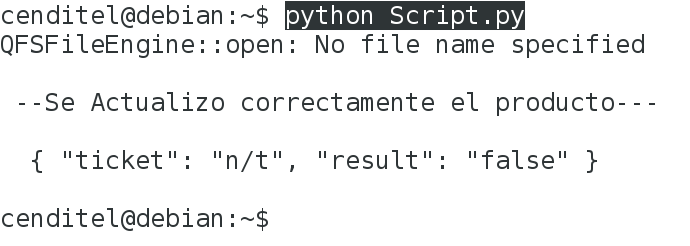
\includegraphics{Modificar.png}\hfill}
\begin{quote}\begin{description}
\item[{Figura 29}] \leavevmode
Script Actualizar producto.

\end{description}\end{quote}
\end{quote}
\begin{itemize}
\item {} 
\textbf{Observen en la db en la siguiente imagen:} Observe la {\hyperref[_templates/Contenido6/Parte2:figura6]{\emph{Figura 26: Tabla productos}}}
\begin{quote}
\begin{figure}[htbp]
\centering
\capstart

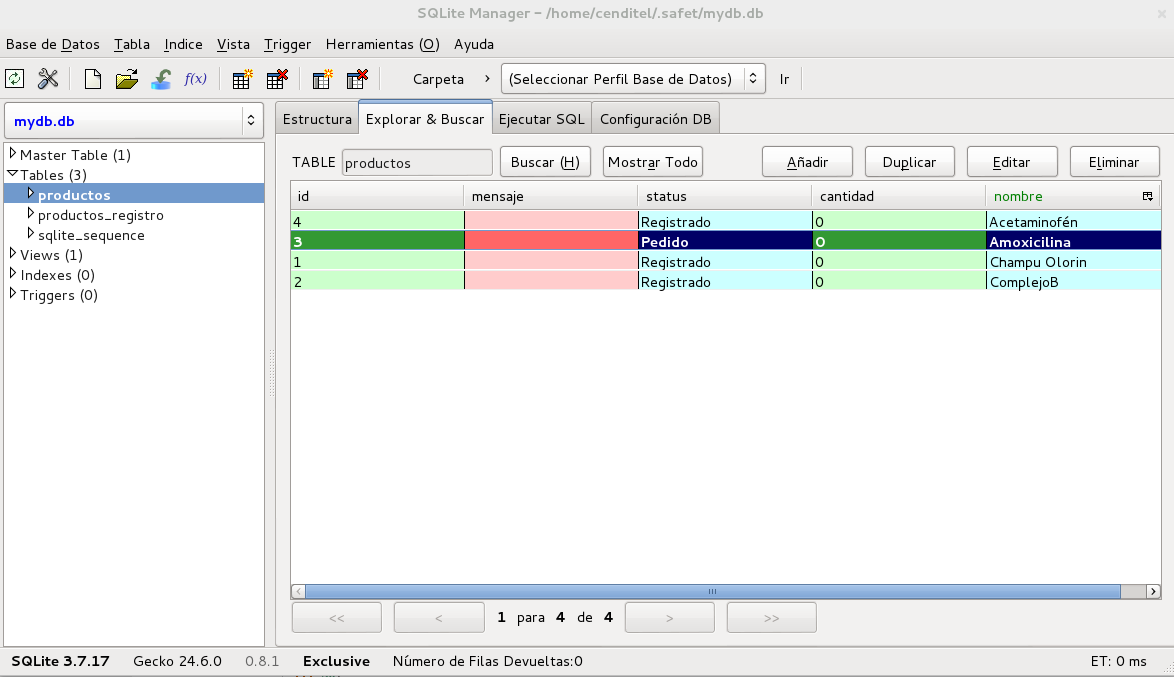
\includegraphics{Modificar1.png}
\caption{\textbf{Figura 26: Tabla productos}}\label{_templates/Contenido6/Parte2:figura6}\end{figure}
\end{quote}

\end{itemize}

\textbf{5.- Operation Actualizar ``Productos'' +(Flujo de trabajo)}
\begin{quote}

\begin{Verbatim}[commandchars=\\\{\}]
\PYGZlt{}operation  name=\PYGZdq{}Actualizar\PYGZus{}producto\PYGZdq{} desc=\PYGZdq{}Pasa de estado un determinado ticket\PYGZdq{} icon=\PYGZdq{}padlock.png\PYGZdq{}\PYGZgt{}

        \PYGZlt{}command id =\PYGZdq{}1\PYGZdq{} type=\PYGZdq{}actualizar\PYGZdq{} table=\PYGZdq{}productos\PYGZdq{}\PYGZgt{}

                \PYGZlt{}fields\PYGZgt{}

                        \PYGZlt{}field type=\PYGZdq{}combolisttable\PYGZdq{} options=\PYGZdq{}id:productos::\PYGZsq{}(\PYGZsq{} \textbar{}\textbar{} id \textbar{}\textbar{} \PYGZsq{})\PYGZsq{} \textbar{}\textbar{}  nombre\PYGZdq{}
                                                        mandatory=\PYGZdq{}yes\PYGZdq{} primarykey=\PYGZdq{}yes\PYGZdq{} order=\PYGZdq{}desc\PYGZdq{}\PYGZgt{}
                        id
                        \PYGZlt{}/field\PYGZgt{}

                        \PYGZlt{}field type=\PYGZdq{}comboflow\PYGZdq{} mandatory=\PYGZdq{}yes\PYGZdq{} options=\PYGZdq{}next\PYGZdq{}
                                path=\PYGZdq{}/home/cenditel/.safet/flowfiles/productos.xml\PYGZdq{} title=\PYGZdq{}Status\PYGZus{}producto\PYGZdq{}\PYGZgt{}
                        status
                        \PYGZlt{}/field\PYGZgt{}

                \PYGZlt{}/fields\PYGZgt{}
        \PYGZlt{}/command\PYGZgt{}

        \PYGZlt{}command id =\PYGZdq{}1\PYGZdq{} type=\PYGZdq{}agregar\PYGZdq{} table=\PYGZdq{}productos\PYGZus{}registro\PYGZdq{} \PYGZgt{}

                \PYGZlt{}fields\PYGZgt{}

                        \PYGZlt{}field type=\PYGZdq{}datetime\PYGZdq{} mandatory=\PYGZdq{}yes\PYGZdq{}  function=\PYGZdq{}seq from sqlite\PYGZus{}sequence where name=\PYGZsq{}productos\PYGZsq{}\PYGZdq{}
                                                                                                                input=\PYGZdq{}no\PYGZdq{}\PYGZgt{}
                         productoid
                        \PYGZlt{}/field\PYGZgt{}

                         \PYGZlt{}field type=\PYGZdq{}datetime\PYGZdq{} mandatory=\PYGZdq{}yes\PYGZdq{}  function=\PYGZdq{}datetime(\PYGZsq{}now\PYGZsq{})\PYGZdq{}
                                                                format=\PYGZdq{}time\PYGZus{}t\PYGZdq{} input=\PYGZdq{}no\PYGZdq{}\PYGZgt{}
                          fecha
                         \PYGZlt{}/field\PYGZgt{}

                         \PYGZlt{}field type=\PYGZdq{}string\PYGZdq{} literal=\PYGZdq{}\PYGZus{}USERNAME\PYGZdq{} mandatory=\PYGZdq{}yes\PYGZdq{} \PYGZgt{}
                          rol
                         \PYGZlt{}/field\PYGZgt{}

                         \PYGZlt{}field type=\PYGZdq{}string\PYGZdq{} title=\PYGZdq{}Status\PYGZdq{}  mandatory=\PYGZdq{}yes\PYGZdq{} \PYGZgt{}
                         regstatus
                         \PYGZlt{}/field\PYGZgt{}

          \PYGZlt{}/fields\PYGZgt{}

        \PYGZlt{}/command\PYGZgt{}

\PYGZlt{}/operation\PYGZgt{}
\end{Verbatim}
\end{quote}
\begin{itemize}
\item {} 
\textbf{Ejecutamos el Script para Actualizar el Status del producto}
\begin{quote}

Seguidamente vamos a utilizar esta operación \textbf{``Actualizar\_producto''} en un Script de python como se muestra a continuación:
\end{quote}

\end{itemize}
\begin{quote}
\begin{itemize}
\item {} 
\textbf{Operación:} Actualizar\_producto

\item {} 
\textbf{id:} Aqui colocaremos el valor de \textbf{id} del producto por ejemplo vamos a actualizar el producto \textbf{Aspirina} y su \textbf{id} es \textbf{3}. Observe la {\hyperref[_templates/Contenido6/Parte2:figura1]{\emph{Figura 26: Tabla productos}}}

\item {} 
\textbf{Estado\_producto:} Aqui se coloca el estado del producto es decir si es por llegar,Agotarse,Pedido,En Espera. En este caso esta \textbf{Registrado} vamos a modificarlo a \textbf{pedido}.

\end{itemize}

\begin{Verbatim}[commandchars=\\\{\}]
\PYG{c}{\PYGZsh{} \PYGZhy{}*\PYGZhy{} coding: utf\PYGZhy{}8 \PYGZhy{}*\PYGZhy{}}

\PYG{c}{\PYGZsh{} C(Insertar)}
\PYG{c}{\PYGZsh{} Agregamos el poducto a ingresar por ejemplo \PYGZdq{}Champu Olorin\PYGZdq{},}
\PYG{c}{\PYGZsh{}                    \PYGZdq{}ComplejoB\PYGZdq{},\PYGZdq{}Aspirina\PYGZdq{},\PYGZdq{}Acetaminofén\PYGZdq{},\PYGZdq{}Ibuprofeno\PYGZdq{}.}
\PYG{c}{\PYGZsh{}myconsult = u\PYGZdq{}operacion:agregar\PYGZus{}producto  Nombre: ComplejoB\PYGZdq{}}

\PYG{c}{\PYGZsh{} D(Borrar o eliminar)}
\PYG{c}{\PYGZsh{} Eliminamos el porducto numero 5}
\PYG{c}{\PYGZsh{}myconsult = u\PYGZdq{}operacion:borrar\PYGZus{}producto id:5\PYGZdq{}}

\PYG{c}{\PYGZsh{} U(Actualizar)}
\PYG{c}{\PYGZsh{} Se actualizara el nombre del producto número 3}
\PYG{c}{\PYGZsh{}myconsult = u\PYGZdq{}operacion:modificar\PYGZus{}producto id:3 Nombre:Amoxicilina\PYGZdq{}}

\PYG{c}{\PYGZsh{} Importación de la librería Safet y os}
\PYG{k+kn}{import} \PYG{n+nn}{Safet}
\PYG{k+kn}{import} \PYG{n+nn}{os}


\PYG{c}{\PYGZsh{} Aqui obtengo mi home,media y url}
\PYG{n}{myhome} \PYG{o}{=} \PYG{n}{os}\PYG{o}{.}\PYG{n}{getenv}\PYG{p}{(}\PYG{l+s}{\PYGZdq{}}\PYG{l+s}{HOME}\PYG{l+s}{\PYGZdq{}}\PYG{p}{)}
\PYG{n}{mymedia} \PYG{o}{=} \PYG{n}{myhome} \PYG{o}{+} \PYG{l+s}{\PYGZdq{}}\PYG{l+s}{/tmp}\PYG{l+s}{\PYGZdq{}}
\PYG{n}{myurl} \PYG{o}{=} \PYG{l+s}{\PYGZdq{}}\PYG{l+s}{http://localhost}\PYG{l+s}{\PYGZdq{}}

 \PYG{c}{\PYGZsh{} Constructor principal}
\PYG{n}{myinflow} \PYG{o}{=} \PYG{n}{Safet}\PYG{o}{.}\PYG{n}{MainWindow}\PYG{p}{(}\PYG{n}{myhome}\PYG{p}{)}

\PYG{n}{myinflow}\PYG{o}{.}\PYG{n}{setMediaPath}\PYG{p}{(}\PYG{n}{mymedia}\PYG{p}{)}
\PYG{n}{myinflow}\PYG{o}{.}\PYG{n}{setHostURL}\PYG{p}{(}\PYG{n}{myurl}\PYG{p}{)}


\PYG{c}{\PYGZsh{} Si no es un usuario registrado el metodo \PYGZdq{}login\PYGZdq{} retorna False}
\PYG{n}{result} \PYG{o}{=} \PYG{n}{myinflow}\PYG{o}{.}\PYG{n}{login}\PYG{p}{(}\PYG{l+s}{\PYGZdq{}}\PYG{l+s}{admin}\PYG{l+s}{\PYGZdq{}}\PYG{p}{,}\PYG{l+s}{\PYGZdq{}}\PYG{l+s}{admin}\PYG{l+s}{\PYGZdq{}}\PYG{p}{)}


\PYG{c}{\PYGZsh{} +(Flujo de trabajo)}
\PYG{c}{\PYGZsh{} Se actualizara su estado}
\PYG{n}{myconsult} \PYG{o}{=} \PYG{l+s}{u\PYGZdq{}}\PYG{l+s}{operacion:Actualizar\PYGZus{}producto id:3 Estado\PYGZus{}producto:Pedido}\PYG{l+s}{\PYGZdq{}}


\PYG{k}{if} \PYG{n}{result}\PYG{p}{:}
        \PYG{n}{result} \PYG{o}{=} \PYG{n}{myinflow}\PYG{o}{.}\PYG{n}{toInputForm}\PYG{p}{(}\PYG{n}{myconsult}\PYG{p}{)}
\PYG{k}{else}\PYG{p}{:}
        \PYG{k}{print} \PYG{l+s}{\PYGZdq{}}\PYG{l+s+se}{\PYGZbs{}n}\PYG{l+s}{ \PYGZhy{}\PYGZhy{}\PYGZhy{}Usuario autenticado\PYGZhy{}\PYGZhy{}\PYGZhy{}}\PYG{l+s+se}{\PYGZbs{}n}\PYG{l+s}{\PYGZdq{}}
        \PYG{n+nb}{exit}\PYG{p}{(}\PYG{p}{)}


\PYG{k}{if} \PYG{n}{result}\PYG{p}{:}
        \PYG{k}{print} \PYG{l+s}{\PYGZdq{}}\PYG{l+s+se}{\PYGZbs{}n}\PYG{l+s}{ \PYGZhy{}\PYGZhy{}Se Actualizo correctamente el producto\PYGZhy{}\PYGZhy{}\PYGZhy{}}\PYG{l+s+se}{\PYGZbs{}n}\PYG{l+s}{\PYGZdq{}}
\PYG{k}{else}\PYG{p}{:}
        \PYG{k}{print} \PYG{l+s}{\PYGZdq{}}\PYG{l+s+se}{\PYGZbs{}n}\PYG{l+s}{ No se Actualizo el producto....!!!}\PYG{l+s+se}{\PYGZbs{}n}\PYG{l+s}{\PYGZdq{}}


\PYG{k}{if} \PYG{o+ow}{not} \PYG{n}{result}\PYG{p}{:}
        \PYG{k}{print} \PYG{l+s}{\PYGZdq{}}\PYG{l+s+se}{\PYGZbs{}n}\PYG{l+s}{Consulta failed error: }\PYG{l+s+si}{\PYGZpc{}s}\PYG{l+s+se}{\PYGZbs{}n}\PYG{l+s}{\PYGZdq{}} \PYG{o}{\PYGZpc{}} \PYG{p}{(}\PYG{n}{myinflow}\PYG{o}{.}\PYG{n}{currentError}\PYG{p}{(}\PYG{p}{)}\PYG{p}{)}
        \PYG{n+nb}{exit}\PYG{p}{(}\PYG{p}{)}

\PYG{k}{print} \PYG{l+s}{u\PYGZdq{}}\PYG{l+s}{  }\PYG{l+s+si}{\PYGZpc{}s}\PYG{l+s+se}{\PYGZbs{}n}\PYG{l+s}{\PYGZdq{}} \PYG{o}{\PYGZpc{}} \PYG{p}{(}\PYG{n}{myinflow}\PYG{o}{.}\PYG{n}{currentJSON}\PYG{p}{(}\PYG{p}{)}\PYG{p}{)}
\end{Verbatim}

\begin{Verbatim}[commandchars=\\\{\}]
\PYGZdl{} python Actualizar\PYGZus{}Status\PYGZus{}producto.py
\end{Verbatim}
\end{quote}

\textbf{Observen la siguiente imagen:}
\begin{quote}

{\hfill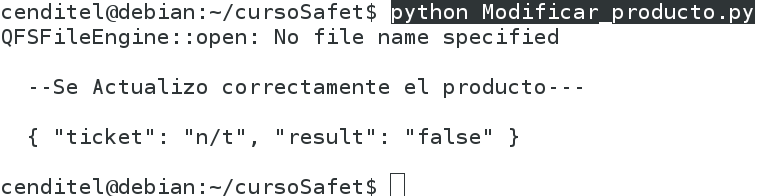
\includegraphics{Actualizar.png}\hfill}
\begin{quote}\begin{description}
\item[{Figura 29}] \leavevmode
Script Actualizar producto.

\end{description}\end{quote}
\end{quote}
\begin{itemize}
\item {} 
\textbf{Observen en la db en la siguiente imagen:} Observe la {\hyperref[_templates/Contenido6/Parte2:figura4]{\emph{Figura 26: Tabla producto}}}
\begin{quote}
\begin{figure}[htbp]
\centering
\capstart

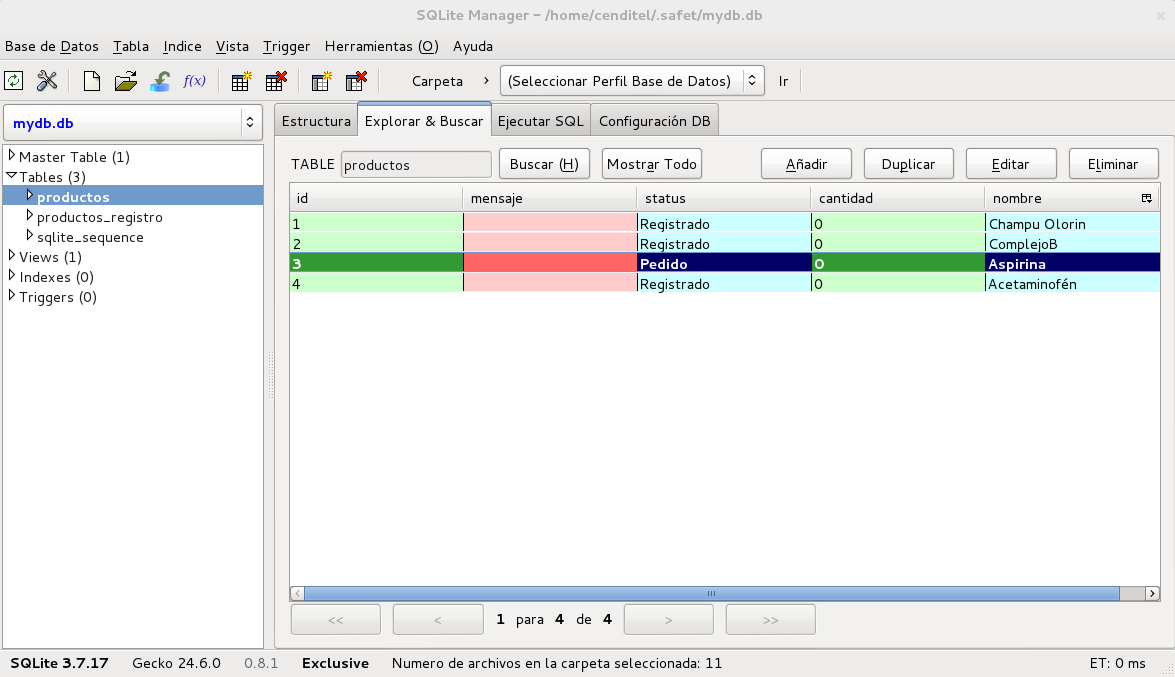
\includegraphics{Actualizar1.png}
\caption{\textbf{Figura 26: Tabla producto}}\label{_templates/Contenido6/Parte2:figura4}\end{figure}
\end{quote}

\item {} 
\textbf{Observen en la db en la siguiente imagen:} Observe la {\hyperref[_templates/Contenido6/Parte2:figura5]{\emph{Figura 27: Tabla producto\_registro}}}
\begin{quote}
\begin{figure}[htbp]
\centering
\capstart

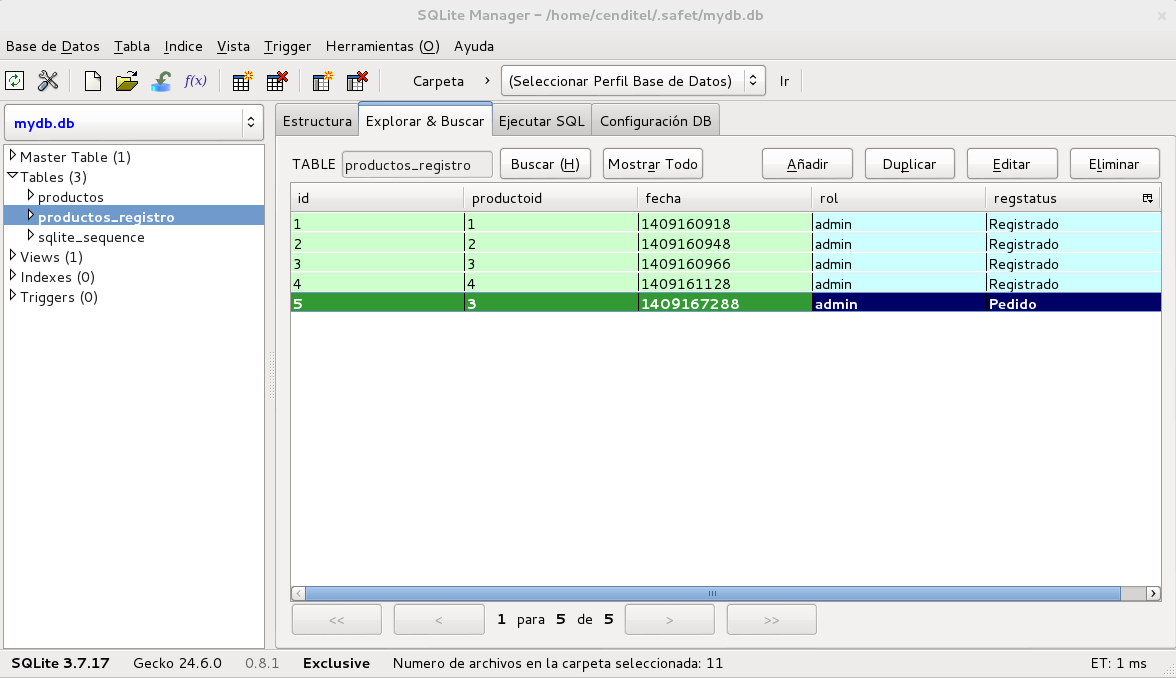
\includegraphics{Actualizar2.png}
\caption{\textbf{Figura 27: Tabla producto\_registro}}\label{_templates/Contenido6/Parte2:figura5}\end{figure}
\end{quote}

\end{itemize}
\begin{description}
\item[{\textbf{Nota:}}] \leavevmode
\begin{Verbatim}[commandchars=\\\{\}]
Si tienen error aquí están los archivos
\end{Verbatim}

\end{description}
\begin{itemize}
\item {} 
Archivo deftrac:
\begin{quote}

\textbf{DOWNLOAD:}


\includegraphics{download1.png}

\code{deftrac.xml}
\end{quote}

\item {} 
Archivo Script:
\begin{quote}

\textbf{DOWNLOAD:}


\includegraphics{download1.png}

\code{Script.py}
\end{quote}

\end{itemize}
\end{quote}


\chapter{\index{Crear el flujo de trabajo utilizando un archivo XML}Crear el flujo de trabajo utilizando un archivo XML}
\label{_templates/Contenido6/Parte4:crear-el-flujo-de-trabajo-utilizando-un-archivo-xml}\label{_templates/Contenido6/Parte4::doc}\begin{quote}

El flujo de trabajo (workflow) es el estudio de los aspectos operacionales de una actividad de trabajo: cómo se estructuran las tareas, cómo se realizan, cuál es su orden correlativo, cómo se sincronizan, cómo fluye la información que soporta las tareas y cómo se le hace seguimiento al cumplimiento de las tareas. Más información \href{http://es.wikipedia.org/wiki/Flujo\_de\_trabajo}{AQUI}.
\end{quote}

\textbf{A continuación seguimos los siguientes paso:}


\section{1° PRIMER PASO}
\label{_templates/Contenido6/Parte4:primer-paso}\begin{itemize}
\item {} 
Crearemos un archivo llamado \textbf{productos.xml}.

\item {} 
Lo guardamos en el siguiente directorio \textbf{\textless{}HOME\textgreater{}.safet/flowfiles/}.

\end{itemize}


\section{2° SEGUNDO PASO}
\label{_templates/Contenido6/Parte4:segundo-paso}

\subsection{Encabezado}
\label{_templates/Contenido6/Parte4:encabezado}\label{_templates/Contenido6/Parte4:id1}\begin{quote}

Abrimos el archivo \textbf{productos.xml} y Escribimos el siguiente encabezado \textbf{(XML)} que aparece en el siguiente block:

\begin{Verbatim}[commandchars=\\\{\}]
\PYG{c+cp}{\PYGZlt{}?xml version=\PYGZsq{}1.0\PYGZsq{} encoding=\PYGZsq{}UTF\PYGZhy{}8\PYGZsq{}?\PYGZgt{}}
\PYG{c+cp}{\PYGZlt{}!DOCTYPE yawl SYSTEM \PYGZsq{}file:///home/cenditel/.safet/dtd/yawlworkflow.dtd\PYGZsq{}\PYGZgt{}}

\PYG{c}{\PYGZlt{}!\PYGZhy{}\PYGZhy{}}
\PYG{c}{Documento  : productos.xml}
\PYG{c}{Creado     : 16/10/08 09:27 AM}
\PYG{c}{Autor      : nombre\PYGZus{}autor}
\PYG{c}{Descripcion: Archivo generado por plantilla de la Libreria SAFET}
\PYG{c}{\PYGZhy{}\PYGZhy{}\PYGZgt{}}
\end{Verbatim}

\begin{notice}{note}{Nota:}
El comentario es opcional.
\end{notice}
\end{quote}


\section{3° TERCER PASO}
\label{_templates/Contenido6/Parte4:tercer-paso}\begin{quote}
\phantomsection\label{_templates/Contenido6/Parte4:tercerpaso}\end{quote}


\subsection{Etiquetas Principales}
\label{_templates/Contenido6/Parte4:tercerpaso}\label{_templates/Contenido6/Parte4:etiquetas-principales}\begin{quote}

En el archivo \textbf{productos.xml} se utilizaran las siguientes \textbf{etiquetas principales (XML)}:
\begin{itemize}
\item {} 
\textbf{\textless{}yawl\textgreater{}:} Etiqueta principal yawl.

\item {} 
\textbf{\textless{}workflow\textgreater{}:} Nombre del flujo.

\item {} 
\textbf{\textless{}token\textgreater{}:} Ficha: Nombre de la tabla  y Nombre del campo.

\end{itemize}

Abrimos el archivo \textbf{productos.xml} y debajo del {\hyperref[_templates/Contenido6/Parte4:encabezado]{\emph{Encabezado}}} copiamos el siguiente código \textbf{(XML)} que aparece en el siguiente block:

\begin{Verbatim}[commandchars=\\\{\}]
\PYG{n+nt}{\PYGZlt{}yawl} \PYG{n+na}{version=}\PYG{l+s}{\PYGZdq{}0.01\PYGZdq{}}\PYG{n+nt}{\PYGZgt{}}
 \PYG{n+nt}{\PYGZlt{}workflow} \PYG{n+na}{id=}\PYG{l+s}{\PYGZdq{}productos\PYGZdq{}}\PYG{n+nt}{\PYGZgt{}}
  \PYG{n+nt}{\PYGZlt{}token} \PYG{n+na}{keysource=}\PYG{l+s}{\PYGZdq{}productos\PYGZdq{}} \PYG{n+na}{key=}\PYG{l+s}{\PYGZdq{}id\PYGZdq{}}\PYG{n+nt}{/\PYGZgt{}}

   \PYG{c}{\PYGZlt{}!\PYGZhy{}\PYGZhy{}}\PYG{c}{  **CUERPO**}
\PYG{c}{    Aqui vamos a colocar todos los estados o tareas.}
\PYG{c}{          \PYGZsh{}\PYGZsh{}\PYGZsh{}\PYGZsh{}\PYGZsh{}\PYGZsh{}\PYGZsh{}\PYGZsh{}\PYGZsh{}\PYGZsh{}\PYGZsh{}\PYGZsh{}\PYGZsh{}\PYGZsh{}\PYGZsh{}\PYGZsh{}\PYGZsh{}\PYGZsh{}\PYGZsh{}\PYGZsh{}\PYGZsh{}\PYGZsh{}\PYGZsh{}\PYGZsh{}\PYGZsh{}}
\PYG{c}{          \PYGZsh{}\PYGZsh{} }\PYG{c}{\PYGZhy{}}\PYG{c}{ INICIAL           \PYGZsh{}\PYGZsh{}}
\PYG{c}{          \PYGZsh{}\PYGZsh{}    }\PYG{c}{\PYGZhy{}}\PYG{c}{ REGISTRADO.    \PYGZsh{}\PYGZsh{}}
\PYG{c}{          \PYGZsh{}\PYGZsh{}    }\PYG{c}{\PYGZhy{}}\PYG{c}{ PEDIDO         \PYGZsh{}\PYGZsh{}}
\PYG{c}{          \PYGZsh{}\PYGZsh{}      }\PYG{c}{\PYGZhy{}}\PYG{c}{ DISPONIBLE   \PYGZsh{}\PYGZsh{}}
\PYG{c}{          \PYGZsh{}\PYGZsh{}      }\PYG{c}{\PYGZhy{}}\PYG{c}{ POR\PYGZus{}LLEGAR   \PYGZsh{}\PYGZsh{}}
\PYG{c}{          \PYGZsh{}\PYGZsh{}    }\PYG{c}{\PYGZhy{}}\PYG{c}{ POR\PYGZus{}AGOTARSE   \PYGZsh{}\PYGZsh{}}
\PYG{c}{          \PYGZsh{}\PYGZsh{}    }\PYG{c}{\PYGZhy{}}\PYG{c}{ AGOSTADO       \PYGZsh{}\PYGZsh{}}
\PYG{c}{          \PYGZsh{}\PYGZsh{} }\PYG{c}{\PYGZhy{}}\PYG{c}{ FINAL             \PYGZsh{}\PYGZsh{}}
\PYG{c}{          \PYGZsh{}\PYGZsh{}\PYGZsh{}\PYGZsh{}\PYGZsh{}\PYGZsh{}\PYGZsh{}\PYGZsh{}\PYGZsh{}\PYGZsh{}\PYGZsh{}\PYGZsh{}\PYGZsh{}\PYGZsh{}\PYGZsh{}\PYGZsh{}\PYGZsh{}\PYGZsh{}\PYGZsh{}\PYGZsh{}\PYGZsh{}\PYGZsh{}\PYGZsh{}\PYGZsh{}\PYGZsh{}}
\PYG{c}{   }\PYG{c}{\PYGZhy{}\PYGZhy{}\PYGZgt{}}

 \PYG{n+nt}{\PYGZlt{}/workflow\PYGZgt{}}
\PYG{n+nt}{\PYGZlt{}/yawl\PYGZgt{}}
\end{Verbatim}

\begin{notice}{note}{Nota:}\begin{itemize}
\item {} 
EL cuadro se me muestra comentado es opcional solo para visualizar como van hacer las tareas.

\item {} 
Todas las tareas o estados van donde esta el cuadro opcional.

\end{itemize}
\end{notice}
\end{quote}


\section{4° CUARTO PASO}
\label{_templates/Contenido6/Parte4:cuarto-paso}\label{_templates/Contenido6/Parte4:cuartopaso}

\subsection{Condiciones Principales (INICIAL Y FINAL)}
\label{_templates/Contenido6/Parte4:condiciones}\label{_templates/Contenido6/Parte4:condiciones-principales-inicial-y-final}\begin{quote}

En las \textbf{condiciones principal (inicial y final)} se utilizaran las siguientes \textbf{etiquetas (XML)}:
\begin{itemize}
\item {} 
\textbf{\textless{}condition\textgreater{}inicial:} Condición inicial

\item {} 
\textbf{\textless{}condition\textgreater{}final:} Condición final

\item {} 
\textbf{\textless{}port\textgreater{} inicial:} Dentro de esta etiqueta van las conexiones continene una conexión.

\item {} 
\textbf{\textless{}port\textgreater{} final:} No tiene a quien conectarse.

\item {} 
\textbf{\textless{}connection\textgreater{} inicial:} Como no hay nada registrado inicio apunta a final

\item {} 
\textbf{\textless{}connection\textgreater{} final:} final no apunta a nada

\end{itemize}

Abrimos el archivo \textbf{productos.xml} y dentro de las {\hyperref[_templates/Contenido6/Parte4:tercerpaso]{\emph{Etiquetas Principales}}} insertamos el siguiente código \textbf{(XML)}  que aparece  en el siguiente block:

\begin{Verbatim}[commandchars=\\\{\}]
\PYG{c}{\PYGZlt{}!\PYGZhy{}\PYGZhy{}}
\PYG{c}{\PYGZsh{}\PYGZsh{}\PYGZsh{}\PYGZsh{}\PYGZsh{}\PYGZsh{}\PYGZsh{}\PYGZsh{}\PYGZsh{}\PYGZsh{}\PYGZsh{}\PYGZsh{}\PYGZsh{}\PYGZsh{}\PYGZsh{}\PYGZsh{}\PYGZsh{}\PYGZsh{}\PYGZsh{}\PYGZsh{}\PYGZsh{}}
\PYG{c}{\PYGZsh{} Condición inicial \PYGZsh{}}
\PYG{c}{\PYGZsh{}\PYGZsh{}\PYGZsh{}\PYGZsh{}\PYGZsh{}\PYGZsh{}\PYGZsh{}\PYGZsh{}\PYGZsh{}\PYGZsh{}\PYGZsh{}\PYGZsh{}\PYGZsh{}\PYGZsh{}\PYGZsh{}\PYGZsh{}\PYGZsh{}\PYGZsh{}\PYGZsh{}\PYGZsh{}\PYGZsh{}}
\PYG{c}{\PYGZhy{}\PYGZhy{}\PYGZgt{}}
  \PYG{n+nt}{\PYGZlt{}condition} \PYG{n+na}{type=}\PYG{l+s}{\PYGZdq{}start\PYGZdq{}} \PYG{n+na}{id=}\PYG{l+s}{\PYGZdq{}inicial\PYGZdq{}}\PYG{n+nt}{\PYGZgt{}}
   \PYG{n+nt}{\PYGZlt{}port} \PYG{n+na}{side=}\PYG{l+s}{\PYGZdq{}forward\PYGZdq{}} \PYG{n+na}{type=}\PYG{l+s}{\PYGZdq{}split\PYGZdq{}}\PYG{n+nt}{\PYGZgt{}}
    \PYG{n+nt}{\PYGZlt{}connection} \PYG{n+na}{query=}\PYG{l+s}{\PYGZdq{}true\PYGZdq{}} \PYG{n+na}{options=}\PYG{l+s}{\PYGZdq{}\PYGZdq{}} \PYG{n+na}{source=}\PYG{l+s}{\PYGZdq{}final\PYGZdq{}}\PYG{n+nt}{/\PYGZgt{}}
   \PYG{n+nt}{\PYGZlt{}/port\PYGZgt{}}
  \PYG{n+nt}{\PYGZlt{}/condition\PYGZgt{}}

\PYG{c}{\PYGZlt{}!\PYGZhy{}\PYGZhy{}}
\PYG{c}{\PYGZsh{}\PYGZsh{}\PYGZsh{}\PYGZsh{}\PYGZsh{}\PYGZsh{}\PYGZsh{}\PYGZsh{}\PYGZsh{}\PYGZsh{}\PYGZsh{}\PYGZsh{}\PYGZsh{}\PYGZsh{}\PYGZsh{}\PYGZsh{}\PYGZsh{}\PYGZsh{}\PYGZsh{}}
\PYG{c}{\PYGZsh{} Condición final \PYGZsh{}}
\PYG{c}{\PYGZsh{}\PYGZsh{}\PYGZsh{}\PYGZsh{}\PYGZsh{}\PYGZsh{}\PYGZsh{}\PYGZsh{}\PYGZsh{}\PYGZsh{}\PYGZsh{}\PYGZsh{}\PYGZsh{}\PYGZsh{}\PYGZsh{}\PYGZsh{}\PYGZsh{}\PYGZsh{}\PYGZsh{}}
\PYG{c}{\PYGZhy{}\PYGZhy{}\PYGZgt{}}
  \PYG{n+nt}{\PYGZlt{}condition} \PYG{n+na}{id=}\PYG{l+s}{\PYGZdq{}final\PYGZdq{}}\PYG{n+nt}{\PYGZgt{}}
   \PYG{n+nt}{\PYGZlt{}port} \PYG{n+na}{side=}\PYG{l+s}{\PYGZdq{}forward\PYGZdq{}} \PYG{n+na}{type=}\PYG{l+s}{\PYGZdq{}split\PYGZdq{}}\PYG{n+nt}{\PYGZgt{}}
    \PYG{n+nt}{\PYGZlt{}connection} \PYG{n+na}{source=}\PYG{l+s}{\PYGZdq{}\PYGZdq{}}\PYG{n+nt}{/\PYGZgt{}}
   \PYG{n+nt}{\PYGZlt{}/port\PYGZgt{}}
  \PYG{n+nt}{\PYGZlt{}/condition\PYGZgt{}}
\end{Verbatim}

\textbf{Ahora ejecutaremos los siguiente pasos:}
\begin{itemize}
\item {} 
Crearemos una carpeta llamada \textbf{tmp} en directorio \textbf{\$HOME/tmp}, desde la consola de comando.

\end{itemize}
\begin{quote}

\begin{Verbatim}[commandchars=\\\{\}]
\PYG{n+nv}{\PYGZdl{} }mkdir \PYG{n+nv}{\PYGZdl{}HOME}/tmp
\end{Verbatim}
\end{quote}
\begin{itemize}
\item {} 
Crearemos un archivo con extensión \textbf{.py} en directorio \textbf{\$HOME},desde la consola de comando.

\end{itemize}
\begin{quote}

\begin{Verbatim}[commandchars=\\\{\}]
\PYG{n+nv}{\PYGZdl{} }touch \PYG{n+nv}{\PYGZdl{}HOME}/Script\PYGZus{}graficos.py
\end{Verbatim}
\end{quote}
\begin{itemize}
\item {} 
Abrimos el archivo \textbf{.py} que creamos en el paso anterior la cual lo llamamos \textbf{Script\_graficos.py} y copiamos el siguiente Script**(python)**:

\end{itemize}
\begin{quote}

\begin{Verbatim}[commandchars=\\\{\}]
\PYG{c}{\PYGZsh{} \PYGZhy{}*\PYGZhy{} coding: utf\PYGZhy{}8 \PYGZhy{}*\PYGZhy{}}

\PYG{k+kn}{import} \PYG{n+nn}{Safet}
\PYG{k+kn}{import} \PYG{n+nn}{os}

\PYG{n}{myhome} \PYG{o}{=} \PYG{n}{os}\PYG{o}{.}\PYG{n}{getenv}\PYG{p}{(}\PYG{l+s}{\PYGZdq{}}\PYG{l+s}{HOME}\PYG{l+s}{\PYGZdq{}}\PYG{p}{)}
\PYG{n}{mymedia} \PYG{o}{=} \PYG{n}{myhome} \PYG{o}{+} \PYG{l+s}{\PYGZdq{}}\PYG{l+s}{/tmp}\PYG{l+s}{\PYGZdq{}}
\PYG{n}{myurl} \PYG{o}{=} \PYG{l+s}{\PYGZdq{}}\PYG{l+s}{http://localhost}\PYG{l+s}{\PYGZdq{}}

\PYG{n}{myinflow} \PYG{o}{=} \PYG{n}{Safet}\PYG{o}{.}\PYG{n}{MainWindow}\PYG{p}{(}\PYG{n}{myhome}\PYG{p}{)}

\PYG{n}{myinflow}\PYG{o}{.}\PYG{n}{setMediaPath}\PYG{p}{(}\PYG{n}{mymedia} \PYG{p}{)}
\PYG{n}{myinflow}\PYG{o}{.}\PYG{n}{setHostURL}\PYG{p}{(}\PYG{n}{myurl}\PYG{p}{)}

\PYG{n}{result} \PYG{o}{=} \PYG{n}{myinflow}\PYG{o}{.}\PYG{n}{login}\PYG{p}{(}\PYG{l+s}{\PYGZdq{}}\PYG{l+s}{admin}\PYG{l+s}{\PYGZdq{}}\PYG{p}{,}\PYG{l+s}{\PYGZdq{}}\PYG{l+s}{admin}\PYG{l+s}{\PYGZdq{}}\PYG{p}{)}

\PYG{n}{myconsult} \PYG{o}{=} \PYG{l+s}{u\PYGZdq{}}\PYG{l+s}{operacion:Generar\PYGZus{}gráfico\PYGZus{}coloreado }\PYG{l+s+se}{\PYGZbs{}}
\PYG{l+s}{        Cargar\PYGZus{}archivo\PYGZus{}flujo: }\PYG{l+s+si}{\PYGZpc{}s}\PYG{l+s}{/.safet/flowfiles/productos.xml}\PYG{l+s}{\PYGZdq{}} \PYG{o}{\PYGZpc{}} \PYG{p}{(}\PYG{n}{myhome}\PYG{p}{)}

\PYG{k}{if} \PYG{o+ow}{not} \PYG{n}{result}\PYG{p}{:}
    \PYG{k}{print} \PYG{l+s}{\PYGZdq{}}\PYG{l+s}{Authentication failed}\PYG{l+s}{\PYGZdq{}}
    \PYG{n+nb}{exit}\PYG{p}{(}\PYG{p}{)}

\PYG{n}{result} \PYG{o}{=} \PYG{n}{myinflow}\PYG{o}{.}\PYG{n}{toInputConsole}\PYG{p}{(}\PYG{n}{myconsult}\PYG{p}{)}

\PYG{k}{if} \PYG{o+ow}{not} \PYG{n}{result}\PYG{p}{:}
    \PYG{k}{print} \PYG{l+s}{\PYGZdq{}}\PYG{l+s}{Consult failed error: }\PYG{l+s+si}{\PYGZpc{}s}\PYG{l+s}{\PYGZdq{}}  \PYG{o}{\PYGZpc{}} \PYG{p}{(}\PYG{n}{myinflow}\PYG{o}{.}\PYG{n}{currentError}\PYG{p}{(}\PYG{p}{)}\PYG{p}{)}
    \PYG{n+nb}{exit}\PYG{p}{(}\PYG{p}{)}

\PYG{k}{print} \PYG{l+s}{u\PYGZdq{}}\PYG{l+s+si}{\PYGZpc{}s}\PYG{l+s}{\PYGZdq{}} \PYG{o}{\PYGZpc{}} \PYG{p}{(}\PYG{n}{myinflow}\PYG{o}{.}\PYG{n}{currentJSON}\PYG{p}{(}\PYG{p}{)}\PYG{p}{)}
\end{Verbatim}
\end{quote}
\begin{itemize}
\item {} 
Ejecutamos el archivo \textbf{Script\_graficos.py}, desde la consola de comando como usuario normal.

\end{itemize}
\begin{quote}

\begin{Verbatim}[commandchars=\\\{\}]
\PYG{n+nv}{\PYGZdl{} }python \PYG{n+nv}{\PYGZdl{}HOME}/Script\PYGZus{}graficos.py
\end{Verbatim}

\begin{notice}{note}{Nota:}
Al ejecutar el archivo \textbf{.py (Script\_graficos.py)} nos mostrara un mensaje donde salen reflejadas las 2 {\hyperref[_templates/Contenido6/Parte4:condiciones]{\emph{Condiciones Principales (INICIAL Y FINAL)}}}:
\begin{quote}

\begin{Verbatim}[commandchars=\\\{\}]
QFSFileEngine::open: No file name specified
QSqlDatabasePrivate::removeDatabase: connection \PYG{l+s+s1}{\PYGZsq{}/home/cenditel/.safet/mydb.db\PYGZsq{}}
is still in use, all queries will cease to work.
.............wheretokens: on
.......newnode: \textbar{}inicial\textbar{}  \PYG{c}{\PYGZsh{} Nueva condición inicial}
.......newnode: \textbar{}final\textbar{}    \PYG{c}{\PYGZsh{} Nueva condición final}
qt\PYGZus{}temp.XM6827.svg         \PYG{c}{\PYGZsh{} Obtenemos la nueva imagen con su nombre la cual contiene el gráfico}
\end{Verbatim}
\end{quote}

\textbf{El nombre de la imagen (.svg) es temporal, es decir su nombre varia constante mente.}
\end{notice}
\end{quote}
\begin{itemize}
\item {} 
Nos vamos al directorio \textbf{\$HOME/tmp},desde la consola de comando.

\end{itemize}
\begin{quote}

\begin{Verbatim}[commandchars=\\\{\}]
\PYG{n+nv}{\PYGZdl{} }\PYG{n+nb}{cd} \PYG{n+nv}{\PYGZdl{}HOME}/tmp
\end{Verbatim}

\begin{notice}{note}{Nota:}
En el directorio \textbf{\$HOME/tmp} se escriben los archivos de grafos \textbf{(.svg o .png)}, usted puede definir el directorio de escritura y temporal utilizando los siguientes parámetros en el archivo \textbf{safet.conf} que se encuentra en el directorio \textbf{\$HOME/.safet/}.

\begin{Verbatim}[commandchars=\\\{\}]
plugins.graphviz.infile \PYG{o}{=}  /home/fulano/tmp   \PYG{c}{\PYGZsh{} directorio para archivos temporales}
plugins.graphviz.outfile \PYG{o}{=}  /home/fulano/tmp  \PYG{c}{\PYGZsh{} directorio de salida para archivos de grafo (.svg o .png)}
\end{Verbatim}
\end{notice}
\end{quote}
\begin{itemize}
\item {} 
Escribimos el comando \textbf{ls} para ver las imágenes \textbf{.svg},desde la consola de comando.

\end{itemize}
\begin{quote}

\begin{Verbatim}[commandchars=\\\{\}]
tmp\PYG{n+nv}{\PYGZdl{} }ls
qt\PYGZus{}temp.XM7929.svg
\end{Verbatim}
\end{quote}
\begin{itemize}
\item {} 
Con el comando \textbf{eog} vemos la primera imagen \textbf{.svg(qt\_temp.XM6827.svg )} ,desde la consola de comando.

\end{itemize}
\begin{quote}

\begin{Verbatim}[commandchars=\\\{\}]
tmp\PYG{n+nv}{\PYGZdl{} }eog qt\PYGZus{}temp.XM6827.svg
\end{Verbatim}

\begin{notice}{note}{Nota:}
Si realizó los pasos correctos se mostrara el grafo, en el cual se define lo siguiente:
\begin{quote}
\begin{figure}[htbp]
\centering
\capstart

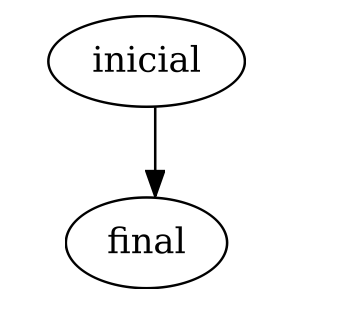
\includegraphics{grafo_inflow.png}
\caption{\textbf{Figura 28: Condiciones (inicial y final).}}\label{_templates/Contenido6/Parte4:figura28}\end{figure}
\end{quote}

Descripción de la {\hyperref[_templates/Contenido6/Parte4:figura28]{\emph{Figura 28: Condiciones (inicial y final).}}}:
\begin{itemize}
\item {} 
El circulo \textbf{inicial} apunta al circulo \textbf{final}.

\item {} 
En este inventario esta vacío.

\item {} 
En esta imagen vemos como se conectan las condiciones \textbf{inicial y final}.

\end{itemize}
\end{notice}

\begin{notice}{note}{Nota:}
En esta imagen no se muestran ninguna tarea ya que no hemos realizado ninguna, para ello pasamos al {\hyperref[_templates/Contenido6/Parte4:quintopaso]{\emph{5° QUINTO PASO}}} donde comenzaremos a realizar las tareas.
\end{notice}
\end{quote}
\end{quote}


\section{5° QUINTO PASO}
\label{_templates/Contenido6/Parte4:quintopaso}\label{_templates/Contenido6/Parte4:quinto-paso}

\subsection{\textbf{5.1 - PRIMERA TAREA (Registrado)}}
\label{_templates/Contenido6/Parte4:primera-tarea-registrado}\begin{quote}

En la primera tarea \textbf{(Registrado)} se utilizaran las siguientes \textbf{etiquetas (XML)}:
\begin{itemize}
\item {} 
\textbf{\textless{}connection\textgreater{}:} \textbf{Registrado} apunta a \textbf{final}, esto varia.

\item {} 
\textbf{\textless{}task\textgreater{}:} Nombre de la tarea \textbf{(Registrado)} y su mensaje.

\item {} 
\textbf{\textless{}port\textgreater{}:} Registrado apunta a una opción.

\item {} 
\textbf{\textless{}variable\textgreater{}:} Variable \textbf{vRegistro} donde me aparecerá un mensaje la hora en el cual se hizo ese registro.

\end{itemize}

Abrimos el archivo \textbf{productos.xml} y insertamos el código \textbf{(xml)} de la \textbf{tarea Registrado} que aparece en el siguiente block:
\begin{quote}

\begin{notice}{note}{Nota:}
La condición \textbf{inicial} se modifico en la etiqueta \textbf{\textless{}connection\textgreater{}} la cual apuntará la tarea \textbf{Registrado}.
\end{notice}
\end{quote}

\begin{Verbatim}[commandchars=\\\{\}]
\PYG{c}{\PYGZlt{}!\PYGZhy{}\PYGZhy{}}
\PYG{c}{*********************}
\PYG{c}{\textbar{} Condición inicial \textbar{}}
\PYG{c}{*********************}
\PYG{c}{\PYGZhy{}\PYGZhy{}\PYGZgt{}}
  \PYG{n+nt}{\PYGZlt{}condition} \PYG{n+na}{type=}\PYG{l+s}{\PYGZdq{}start\PYGZdq{}} \PYG{n+na}{id=}\PYG{l+s}{\PYGZdq{}inicial\PYGZdq{}}\PYG{n+nt}{\PYGZgt{}}
   \PYG{n+nt}{\PYGZlt{}port} \PYG{n+na}{side=}\PYG{l+s}{\PYGZdq{}forward\PYGZdq{}} \PYG{n+na}{type=}\PYG{l+s}{\PYGZdq{}split\PYGZdq{}}\PYG{n+nt}{\PYGZgt{}}
    \PYG{n+nt}{\PYGZlt{}connection} \PYG{n+na}{query=}\PYG{l+s}{\PYGZdq{}select status from productos\PYGZdq{}} \PYG{n+na}{options=}\PYG{l+s}{\PYGZdq{}Registrado\PYGZdq{}} \PYG{n+na}{source=}\PYG{l+s}{\PYGZdq{}Registrado\PYGZdq{}}\PYG{n+nt}{/\PYGZgt{}}
   \PYG{n+nt}{\PYGZlt{}/port\PYGZgt{}}
  \PYG{n+nt}{\PYGZlt{}/condition\PYGZgt{}}


  \PYG{c}{\PYGZlt{}!\PYGZhy{}\PYGZhy{}}
\PYG{c}{  **************}
\PYG{c}{  \textbar{} Registrado \textbar{}}
\PYG{c}{  **************}
\PYG{c}{  }\PYG{c}{\PYGZhy{}\PYGZhy{}\PYGZgt{}}
  \PYG{n+nt}{\PYGZlt{}task} \PYG{n+na}{title=}\PYG{l+s}{\PYGZdq{}en inventario\PYGZdq{}} \PYG{n+na}{id=}\PYG{l+s}{\PYGZdq{}Registrado\PYGZdq{}}\PYG{n+nt}{\PYGZgt{}}
   \PYG{n+nt}{\PYGZlt{}port} \PYG{n+na}{side=}\PYG{l+s}{\PYGZdq{}forward\PYGZdq{}} \PYG{n+na}{type=}\PYG{l+s}{\PYGZdq{}split\PYGZdq{}}\PYG{n+nt}{\PYGZgt{}}
    \PYG{n+nt}{\PYGZlt{}connection} \PYG{n+na}{query=}\PYG{l+s}{\PYGZdq{}true\PYGZdq{}} \PYG{n+na}{options=}\PYG{l+s}{\PYGZdq{}\PYGZdq{}} \PYG{n+na}{source=}\PYG{l+s}{\PYGZdq{}final\PYGZdq{}}\PYG{n+nt}{/\PYGZgt{}}
   \PYG{n+nt}{\PYGZlt{}/port\PYGZgt{}}
   \PYG{n+nt}{\PYGZlt{}variable} \PYG{n+na}{config=}\PYG{l+s}{\PYGZdq{}1\PYGZdq{}} \PYG{n+na}{documentsource=}\PYG{l+s}{\PYGZdq{}select id,nombre,status from productos\PYGZdq{}} \PYG{n+na}{type=}\PYG{l+s}{\PYGZdq{}sql\PYGZdq{}} \PYG{n+na}{tokenlink=}\PYG{l+s}{\PYGZdq{}\PYGZdq{}}
    \PYG{n+na}{id=}\PYG{l+s}{\PYGZdq{}vRegistrado\PYGZdq{}} \PYG{n+na}{rolfield=}\PYG{l+s}{\PYGZdq{}(select rol from productos\PYGZus{}registro}
\PYG{l+s}{    where productoid=productos.id and regstatus=\PYGZsq{}Registrado\PYGZsq{}) as rol\PYGZdq{}} \PYG{n+na}{scope=}\PYG{l+s}{\PYGZdq{}task\PYGZdq{}}
    \PYG{n+na}{timestampfield=}\PYG{l+s}{\PYGZdq{}(select fecha from productos\PYGZus{}registro}
\PYG{l+s}{    where productoid=productos.id and regstatus=\PYGZsq{}Registrado\PYGZsq{}) as fecha\PYGZdq{}}\PYG{n+nt}{/\PYGZgt{}}
  \PYG{n+nt}{\PYGZlt{}/task\PYGZgt{}}


\PYG{c}{\PYGZlt{}!\PYGZhy{}\PYGZhy{}}
\PYG{c}{*******************}
\PYG{c}{\textbar{} Condición final \textbar{}}
\PYG{c}{*******************}
\PYG{c}{\PYGZhy{}\PYGZhy{}\PYGZgt{}}
  \PYG{n+nt}{\PYGZlt{}condition} \PYG{n+na}{id=}\PYG{l+s}{\PYGZdq{}final\PYGZdq{}}\PYG{n+nt}{\PYGZgt{}}
   \PYG{n+nt}{\PYGZlt{}port} \PYG{n+na}{side=}\PYG{l+s}{\PYGZdq{}forward\PYGZdq{}} \PYG{n+na}{type=}\PYG{l+s}{\PYGZdq{}split\PYGZdq{}}\PYG{n+nt}{\PYGZgt{}}
    \PYG{n+nt}{\PYGZlt{}connection} \PYG{n+na}{source=}\PYG{l+s}{\PYGZdq{}\PYGZdq{}}\PYG{n+nt}{/\PYGZgt{}}
   \PYG{n+nt}{\PYGZlt{}/port\PYGZgt{}}
  \PYG{n+nt}{\PYGZlt{}/condition\PYGZgt{}}
\end{Verbatim}

\textbf{Ahora ejecutaremos los siguiente pasos:}

\begin{notice}{note}{Nota:}
En el {\hyperref[_templates/Contenido6/Parte4:cuartopaso]{\emph{4° CUARTO PASO}}} creamos la carpeta llamada \textbf{tmp} y el archivo llamado \textbf{.py (Script\_graficos.py)} ,la cual se utilizaran en este paso a seguir.
\end{notice}
\begin{itemize}
\item {} 
Ejecutamos el mismo archivo \textbf{.py (Script\_graficos.py)} con el mismo contenido, desde la consola de comando como usuario normal.

\end{itemize}
\begin{quote}

\begin{Verbatim}[commandchars=\\\{\}]
\PYG{n+nv}{\PYGZdl{} }python \PYG{n+nv}{\PYGZdl{}HOME}/Script\PYGZus{}graficos.py
\end{Verbatim}

\begin{notice}{note}{Nota:}
Al ejecutar el archivo \textbf{.py (Script\_graficos.py)} nos mostrara un mensaje donde salen reflejadas las 2 \textbf{Condiciones principales} y la primera tarea \textbf{(Registrado)}:
\begin{quote}

\begin{Verbatim}[commandchars=\\\{\}]
QFSFileEngine::open: No file name specified
QSqlDatabasePrivate::removeDatabase: connection \PYG{l+s+s1}{\PYGZsq{}/home/cenditel/.safet/mydb.db\PYGZsq{}}
is still in use, all queries will cease to work.
.............wheretokens: on
.......newnode: \textbar{}Registrado\textbar{} \PYG{c}{\PYGZsh{} Nueva tarea Registrado}
.......newnode: \textbar{}inicial\textbar{}    \PYG{c}{\PYGZsh{} Condición inicial}
.......newnode: \textbar{}final\textbar{}      \PYG{c}{\PYGZsh{} Condición final}
qt\PYGZus{}temp.XM6827.svg           \PYG{c}{\PYGZsh{} Obtenemos la nueva imagen con su nombre la cual contiene el gráfico}
\end{Verbatim}
\end{quote}

\textbf{El nombre de la imagen (.svg) es temporal, es decir su nombre varia constante mente.}
\end{notice}

\begin{notice}{note}{Nota:}
El nombre de la imagen (.svg) es temporal, es decir su nombre varia constante mente.
\end{notice}
\end{quote}
\begin{itemize}
\item {} 
Nos vamos al directorio \textbf{\$HOME/tmp},desde la consola de comando.

\end{itemize}
\begin{quote}

\begin{Verbatim}[commandchars=\\\{\}]
\PYG{n+nv}{\PYGZdl{} }\PYG{n+nb}{cd} \PYG{n+nv}{\PYGZdl{}HOME}/tmp
\end{Verbatim}
\end{quote}
\begin{itemize}
\item {} 
Escribimos el comando \textbf{ls} para ver las 2 imágenes \textbf{.svg} que hemos obtenido ,desde la consola de comando.

\end{itemize}
\begin{quote}

\begin{Verbatim}[commandchars=\\\{\}]
tmp\PYG{n+nv}{\PYGZdl{} }ls
qt\PYGZus{}temp.XM6827.svg ,qt\PYGZus{}temp.XM6970.svg
\end{Verbatim}
\end{quote}
\begin{itemize}
\item {} 
Con el comando \textbf{eog} vemos la la segunda imagen \textbf{.svg(qt\_temp.XM6827.svg )} ,desde la consola de comando.

\end{itemize}
\begin{quote}

\begin{Verbatim}[commandchars=\\\{\}]
tmp\PYG{n+nv}{\PYGZdl{} }eog qt\PYGZus{}temp.XM6970.svg
\end{Verbatim}

\begin{notice}{note}{Nota:}
Si realizó los pasos correctos, se mostrara el grafo como en la imagen siguiente {\hyperref[_templates/Contenido6/Parte4:figura29]{\emph{Figura 29: Registrado}}}:
\begin{quote}
\begin{figure}[htbp]
\centering
\capstart

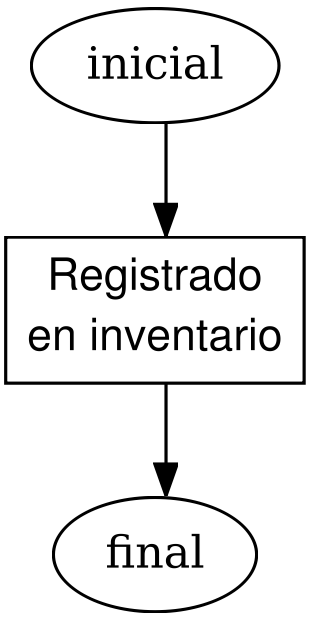
\includegraphics{grafo_inflow1.png}
\caption{\textbf{Figura 29: Registrado}}\label{_templates/Contenido6/Parte4:figura29}\end{figure}
\end{quote}

Descripción de la {\hyperref[_templates/Contenido6/Parte4:figura29]{\emph{Figura 29: Registrado}}}:
\begin{itemize}
\item {} 
La condición del circulo \textbf{inicial} apunta a la primera tarea de cuadro \textbf{Registrado}.

\item {} 
La primera tarea \textbf{Registrado} apunta a la condición de circulo \textbf{final}

\item {} 
En esta imagen vemos como se conectan la condición  \textbf{inicial} con la primera tarea \textbf{Registrado}  y la tarea con la condición \textbf{final}.

\end{itemize}
\end{notice}
\end{quote}
\end{quote}


\subsection{\textbf{5.2 - SEGUNDA TAREA (Pedido)}}
\label{_templates/Contenido6/Parte4:segunda-tarea-pedido}\begin{quote}

En la  segunda tarea \textbf{(Pedido)} se utilizaran las siguientes \textbf{etiquetas (XML)}:
\begin{itemize}
\item {} 
\textbf{\textless{}connection\textgreater{}:} \textbf{Pedido} apunta a \textbf{final}, esto varia.

\item {} 
\textbf{\textless{}task\textgreater{}:} Nombre de la tarea \textbf{(Pedido)}

\item {} 
\textbf{\textless{}port\textgreater{}:} \textbf{Pedido} apunta a dos opciones con el operador \textbf{OR}.

\item {} 
\textbf{\textless{}variable\textgreater{}:} Variable \textbf{vPedido} donde me aparecerá un mensaje la hora en el cual se hizo ese pedido.

\end{itemize}

Abrimos el archivo \textbf{productos.xml} y insertamos el código \textbf{(xml)} de la \textbf{tarea Pedido} que aparece en el siguiente block:
\begin{quote}

\begin{notice}{note}{Nota:}
La tarea \textbf{Registrado} se modifico en la etiqueta \textbf{\textless{}connection\textgreater{}} la cual apuntará a la tarea \textbf{Pedido}.
\end{notice}
\end{quote}

\begin{Verbatim}[commandchars=\\\{\}]
\PYG{c}{\PYGZlt{}!\PYGZhy{}\PYGZhy{}}
\PYG{c}{*********************}
\PYG{c}{\textbar{} Condición inicial \textbar{}}
\PYG{c}{*********************}
\PYG{c}{\PYGZhy{}\PYGZhy{}\PYGZgt{}}
  \PYG{n+nt}{\PYGZlt{}condition} \PYG{n+na}{type=}\PYG{l+s}{\PYGZdq{}start\PYGZdq{}} \PYG{n+na}{id=}\PYG{l+s}{\PYGZdq{}inicial\PYGZdq{}}\PYG{n+nt}{\PYGZgt{}}
   \PYG{n+nt}{\PYGZlt{}port} \PYG{n+na}{side=}\PYG{l+s}{\PYGZdq{}forward\PYGZdq{}} \PYG{n+na}{type=}\PYG{l+s}{\PYGZdq{}split\PYGZdq{}}\PYG{n+nt}{\PYGZgt{}}
    \PYG{n+nt}{\PYGZlt{}connection} \PYG{n+na}{query=}\PYG{l+s}{\PYGZdq{}select status from productos\PYGZdq{}} \PYG{n+na}{options=}\PYG{l+s}{\PYGZdq{}Registrado\PYGZdq{}} \PYG{n+na}{source=}\PYG{l+s}{\PYGZdq{}Registrado\PYGZdq{}}\PYG{n+nt}{/\PYGZgt{}}
   \PYG{n+nt}{\PYGZlt{}/port\PYGZgt{}}
  \PYG{n+nt}{\PYGZlt{}/condition\PYGZgt{}}


  \PYG{c}{\PYGZlt{}!\PYGZhy{}\PYGZhy{}}
\PYG{c}{  **************}
\PYG{c}{  \textbar{} Registrado \textbar{}}
\PYG{c}{  **************}
\PYG{c}{  }\PYG{c}{\PYGZhy{}\PYGZhy{}\PYGZgt{}}
  \PYG{n+nt}{\PYGZlt{}task} \PYG{n+na}{title=}\PYG{l+s}{\PYGZdq{}en inventario\PYGZdq{}} \PYG{n+na}{id=}\PYG{l+s}{\PYGZdq{}Registrado\PYGZdq{}}\PYG{n+nt}{\PYGZgt{}}
   \PYG{n+nt}{\PYGZlt{}port} \PYG{n+na}{side=}\PYG{l+s}{\PYGZdq{}forward\PYGZdq{}} \PYG{n+na}{type=}\PYG{l+s}{\PYGZdq{}split\PYGZdq{}}\PYG{n+nt}{\PYGZgt{}}
    \PYG{n+nt}{\PYGZlt{}connection} \PYG{n+na}{query=}\PYG{l+s}{\PYGZdq{}select status from productos\PYGZdq{}} \PYG{n+na}{options=}\PYG{l+s}{\PYGZdq{}Pedido\PYGZdq{}} \PYG{n+na}{source=}\PYG{l+s}{\PYGZdq{}Pedido\PYGZdq{}}\PYG{n+nt}{/\PYGZgt{}}
   \PYG{n+nt}{\PYGZlt{}/port\PYGZgt{}}
   \PYG{n+nt}{\PYGZlt{}variable} \PYG{n+na}{config=}\PYG{l+s}{\PYGZdq{}1\PYGZdq{}} \PYG{n+na}{documentsource=}\PYG{l+s}{\PYGZdq{}select id,nombre,status from productos\PYGZdq{}} \PYG{n+na}{type=}\PYG{l+s}{\PYGZdq{}sql\PYGZdq{}} \PYG{n+na}{tokenlink=}\PYG{l+s}{\PYGZdq{}\PYGZdq{}}
    \PYG{n+na}{id=}\PYG{l+s}{\PYGZdq{}vRegistrado\PYGZdq{}} \PYG{n+na}{rolfield=}\PYG{l+s}{\PYGZdq{}(select rol from productos\PYGZus{}registro}
\PYG{l+s}{    where productoid=productos.id and regstatus=\PYGZsq{}Registrado\PYGZsq{}) as rol\PYGZdq{}} \PYG{n+na}{scope=}\PYG{l+s}{\PYGZdq{}task\PYGZdq{}}
    \PYG{n+na}{timestampfield=}\PYG{l+s}{\PYGZdq{}(select fecha from productos\PYGZus{}registro}
\PYG{l+s}{    where productoid=productos.id and regstatus=\PYGZsq{}Registrado\PYGZsq{}) as fecha\PYGZdq{}}\PYG{n+nt}{/\PYGZgt{}}
  \PYG{n+nt}{\PYGZlt{}/task\PYGZgt{}}


  \PYG{c}{\PYGZlt{}!\PYGZhy{}\PYGZhy{}}
\PYG{c}{  **********}
\PYG{c}{  \textbar{} Pedido \textbar{}}
\PYG{c}{  **********}
\PYG{c}{  }\PYG{c}{\PYGZhy{}\PYGZhy{}\PYGZgt{}}
  \PYG{n+nt}{\PYGZlt{}task} \PYG{n+na}{title=}\PYG{l+s}{\PYGZdq{}\PYGZdq{}} \PYG{n+na}{id=}\PYG{l+s}{\PYGZdq{}Pedido\PYGZdq{}} \PYG{n+na}{textualinfo=}\PYG{l+s}{\PYGZdq{}\PYGZdq{}}\PYG{n+nt}{\PYGZgt{}}
   \PYG{n+nt}{\PYGZlt{}port} \PYG{n+na}{pattern=}\PYG{l+s}{\PYGZdq{}none\PYGZdq{}} \PYG{n+na}{side=}\PYG{l+s}{\PYGZdq{}forward\PYGZdq{}} \PYG{n+na}{type=}\PYG{l+s}{\PYGZdq{}split\PYGZdq{}}\PYG{n+nt}{\PYGZgt{}}
    \PYG{n+nt}{\PYGZlt{}connection} \PYG{n+na}{query=}\PYG{l+s}{\PYGZdq{}true\PYGZdq{}} \PYG{n+na}{options=}\PYG{l+s}{\PYGZdq{}\PYGZdq{}} \PYG{n+na}{source=}\PYG{l+s}{\PYGZdq{}final\PYGZdq{}}\PYG{n+nt}{/\PYGZgt{}}
   \PYG{n+nt}{\PYGZlt{}/port\PYGZgt{}}
   \PYG{n+nt}{\PYGZlt{}variable} \PYG{n+na}{config=}\PYG{l+s}{\PYGZdq{}1\PYGZdq{}} \PYG{n+na}{documentsource=}\PYG{l+s}{\PYGZdq{}select id,nombre,status from productos\PYGZdq{}} \PYG{n+na}{type=}\PYG{l+s}{\PYGZdq{}sql\PYGZdq{}} \PYG{n+na}{tokenlink=}\PYG{l+s}{\PYGZdq{}\PYGZdq{}}
    \PYG{n+na}{id=}\PYG{l+s}{\PYGZdq{}vPedido\PYGZdq{}} \PYG{n+na}{rolfield=}\PYG{l+s}{\PYGZdq{}(select rol from\PYGZam{}\PYGZsh{}xa;productos\PYGZus{}registro}
\PYG{l+s}{    where productoid=productos.id and regstatus=\PYGZsq{}Pedido\PYGZsq{}) as rol\PYGZdq{}} \PYG{n+na}{scope=}\PYG{l+s}{\PYGZdq{}task\PYGZdq{}}
    \PYG{n+na}{timestampfield=}\PYG{l+s}{\PYGZdq{}(select fecha from productos\PYGZus{}registro}
\PYG{l+s}{    where productoid=productos.id and regstatus=\PYGZsq{}Pedido\PYGZsq{}) as fecha\PYGZdq{}}\PYG{n+nt}{/\PYGZgt{}}
  \PYG{n+nt}{\PYGZlt{}/task\PYGZgt{}}


\PYG{c}{\PYGZlt{}!\PYGZhy{}\PYGZhy{}}
\PYG{c}{*******************}
\PYG{c}{\textbar{} Condición final \textbar{}}
\PYG{c}{*******************}
\PYG{c}{\PYGZhy{}\PYGZhy{}\PYGZgt{}}
  \PYG{n+nt}{\PYGZlt{}condition} \PYG{n+na}{id=}\PYG{l+s}{\PYGZdq{}final\PYGZdq{}}\PYG{n+nt}{\PYGZgt{}}
   \PYG{n+nt}{\PYGZlt{}port} \PYG{n+na}{side=}\PYG{l+s}{\PYGZdq{}forward\PYGZdq{}} \PYG{n+na}{type=}\PYG{l+s}{\PYGZdq{}split\PYGZdq{}}\PYG{n+nt}{\PYGZgt{}}
    \PYG{n+nt}{\PYGZlt{}connection} \PYG{n+na}{source=}\PYG{l+s}{\PYGZdq{}\PYGZdq{}}\PYG{n+nt}{/\PYGZgt{}}
   \PYG{n+nt}{\PYGZlt{}/port\PYGZgt{}}
  \PYG{n+nt}{\PYGZlt{}/condition\PYGZgt{}}
\end{Verbatim}

\textbf{Ahora ejecutaremos los siguiente pasos:}

\begin{notice}{note}{Nota:}
En el {\hyperref[_templates/Contenido6/Parte4:cuartopaso]{\emph{4° CUARTO PASO}}} creamos la carpeta llamada \textbf{tmp} y el archivo llamado \textbf{.py (Script\_graficos.py)} ,la cual se utilizaran en este paso a seguir.
\end{notice}
\begin{itemize}
\item {} 
Ejecutamos el mismo archivo \textbf{.py (Script\_graficos.py)} con el mismo contenido, desde la consola de comando como usuario normal.

\end{itemize}
\begin{quote}

\begin{Verbatim}[commandchars=\\\{\}]
\PYG{n+nv}{\PYGZdl{} }python \PYG{n+nv}{\PYGZdl{}HOME}/Script\PYGZus{}graficos.py
\end{Verbatim}

\begin{notice}{note}{Nota:}
Al ejecutar el archivo \textbf{.py (Script\_graficos.py)} nos mostrara un mensaje donde salen reflejadas las 2 \textbf{Condiciones principales} y la dos tarea \textbf{(Registrado),(Pedido)}:
\begin{quote}

\begin{Verbatim}[commandchars=\\\{\}]
QFSFileEngine::open: No file name specified
QSqlDatabasePrivate::removeDatabase: connection \PYG{l+s+s1}{\PYGZsq{}/home/cenditel/.safet/mydb.db\PYGZsq{}}
is still in use, all queries will cease to work.
.............wheretokens: on
.......newnode: \textbar{}Pedido\textbar{}     \PYG{c}{\PYGZsh{} Nueva tarea Pedido}
.......newnode: \textbar{}Registrado\textbar{} \PYG{c}{\PYGZsh{} Tarea Registrado}
.......newnode: \textbar{}inicial\textbar{}    \PYG{c}{\PYGZsh{} Condición inicial}
.......newnode: \textbar{}final\textbar{}      \PYG{c}{\PYGZsh{} Condición final}
qt\PYGZus{}temp.XM5792.svg           \PYG{c}{\PYGZsh{} Obtenemos la nueva imagen con su nombre la cual contiene el gráfico}
\end{Verbatim}
\end{quote}

\textbf{El nombre de la imagen (.svg) es temporal, es decir su nombre varia constante mente.}
\end{notice}

\begin{notice}{note}{Nota:}
El nombre de la imagen (.svg) es temporal, es decir su nombre varia constante mente.
\end{notice}
\end{quote}
\begin{itemize}
\item {} 
Nos vamos al directorio \textbf{\$HOME/tmp},desde la consola de comando.

\end{itemize}
\begin{quote}

\begin{Verbatim}[commandchars=\\\{\}]
\PYG{n+nv}{\PYGZdl{} }\PYG{n+nb}{cd} \PYG{n+nv}{\PYGZdl{}HOME}/tmp
\end{Verbatim}
\end{quote}
\begin{itemize}
\item {} 
Escribimos el comando \textbf{ls} para ver las 3 imágenes \textbf{.svg} que hemos obtenido ,desde la consola de comando.

\end{itemize}
\begin{quote}

\begin{Verbatim}[commandchars=\\\{\}]
tmp\PYG{n+nv}{\PYGZdl{} }ls
qt\PYGZus{}temp.XM6827.svg, qt\PYGZus{}temp.XM6970.svg, qt\PYGZus{}temp.XM5792.svg
\end{Verbatim}
\end{quote}
\begin{itemize}
\item {} 
Con el comando \textbf{eog} vemos la tercera imagen \textbf{.svg(qt\_temp.XM5792.svg)} ,desde la consola de comando.

\end{itemize}
\begin{quote}

\begin{Verbatim}[commandchars=\\\{\}]
tmp\PYG{n+nv}{\PYGZdl{} }eog qt\PYGZus{}temp.XM5792.svg
\end{Verbatim}

\begin{notice}{note}{Nota:}
Si realizó los pasos correctos, se mostrara el grafo como en la imagen siguiente {\hyperref[_templates/Contenido6/Parte4:figura30]{\emph{Figura 30: Pedido}}}:
\begin{quote}
\begin{figure}[htbp]
\centering
\capstart

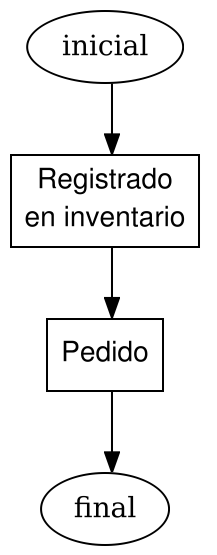
\includegraphics{grafo_inflow2.png}
\caption{\textbf{Figura 30: Pedido}}\label{_templates/Contenido6/Parte4:figura30}\end{figure}
\end{quote}

Descripción de la {\hyperref[_templates/Contenido6/Parte4:figura30]{\emph{Figura 30: Pedido}}}:
\begin{itemize}
\item {} 
La condición del circulo \textbf{inicial} apunta a la primera tarea de cuadro \textbf{Registrado}.

\item {} 
La primera tarea \textbf{Registrado} apunta a la segunda tarea \textbf{Pedido}.

\item {} 
La segunda tarea apunta a la condición de circulo \textbf{final}

\item {} 
En esta imagen vemos como se conectan la condición  \textbf{inicial} con la primera tarea \textbf{Registrado}, la tarea primera tarea con la segunda tarea \textbf{Pedido} y la segunda tarea con la condición \textbf{final}.

\end{itemize}
\end{notice}
\end{quote}
\end{quote}


\subsection{\textbf{5.3 - TERCERA TAREA (Disponible)}}
\label{_templates/Contenido6/Parte4:tercera-tarea-disponible}\begin{quote}

En la  tercera tarea \textbf{(Disponible)} se utilizaran las siguientes \textbf{etiquetas (XML)}:
\begin{itemize}
\item {} 
\textbf{\textless{}task\textgreater{}:} Nombre de la tarea \textbf{(Diponible)}.

\item {} 
\textbf{\textless{}port\textgreater{}:} Disponible apunta a una opción.

\item {} 
\textbf{\textless{}connection\textgreater{}}: \textbf{Disponible} apunta a \textbf{final}, esto varia.

\item {} 
\textbf{\textless{}variable\textgreater{}:} Variable \textbf{vDisponible} donde nos aparecerá \textbf{(nombre,id,status,fecha y hora)} de esa acción.

\end{itemize}

Abrimos el archivo \textbf{productos.xml} y insertamos el código \textbf{(xml)} de la \textbf{tarea Disponible} que aparece en el siguiente block:
\begin{quote}

\begin{notice}{note}{Nota:}
La tarea \textbf{Pedido} se modifico las etiqueta \textbf{\textless{}port\textgreater{}} donde indicará que habran 2 opciones a ocurrir y la etiqueta \textbf{\textless{}connection\textgreater{}} la cual apuntará a la tarea \textbf{Disponible}.
\end{notice}
\end{quote}

\begin{Verbatim}[commandchars=\\\{\}]
\PYG{c}{\PYGZlt{}!\PYGZhy{}\PYGZhy{}}
\PYG{c}{*********************}
\PYG{c}{\textbar{} Condición inicial \textbar{}}
\PYG{c}{*********************}
\PYG{c}{\PYGZhy{}\PYGZhy{}\PYGZgt{}}
  \PYG{n+nt}{\PYGZlt{}condition} \PYG{n+na}{type=}\PYG{l+s}{\PYGZdq{}start\PYGZdq{}} \PYG{n+na}{id=}\PYG{l+s}{\PYGZdq{}inicial\PYGZdq{}}\PYG{n+nt}{\PYGZgt{}}
   \PYG{n+nt}{\PYGZlt{}port} \PYG{n+na}{side=}\PYG{l+s}{\PYGZdq{}forward\PYGZdq{}} \PYG{n+na}{type=}\PYG{l+s}{\PYGZdq{}split\PYGZdq{}}\PYG{n+nt}{\PYGZgt{}}
    \PYG{n+nt}{\PYGZlt{}connection} \PYG{n+na}{query=}\PYG{l+s}{\PYGZdq{}select status from productos\PYGZdq{}} \PYG{n+na}{options=}\PYG{l+s}{\PYGZdq{}Registrado\PYGZdq{}} \PYG{n+na}{source=}\PYG{l+s}{\PYGZdq{}Registrado\PYGZdq{}}\PYG{n+nt}{/\PYGZgt{}}
   \PYG{n+nt}{\PYGZlt{}/port\PYGZgt{}}
  \PYG{n+nt}{\PYGZlt{}/condition\PYGZgt{}}


  \PYG{c}{\PYGZlt{}!\PYGZhy{}\PYGZhy{}}
\PYG{c}{  **************}
\PYG{c}{  \textbar{} Registrado \textbar{}}
\PYG{c}{  **************}
\PYG{c}{  }\PYG{c}{\PYGZhy{}\PYGZhy{}\PYGZgt{}}
  \PYG{n+nt}{\PYGZlt{}task} \PYG{n+na}{title=}\PYG{l+s}{\PYGZdq{}en inventario\PYGZdq{}} \PYG{n+na}{id=}\PYG{l+s}{\PYGZdq{}Registrado\PYGZdq{}}\PYG{n+nt}{\PYGZgt{}}
   \PYG{n+nt}{\PYGZlt{}port} \PYG{n+na}{side=}\PYG{l+s}{\PYGZdq{}forward\PYGZdq{}} \PYG{n+na}{type=}\PYG{l+s}{\PYGZdq{}split\PYGZdq{}}\PYG{n+nt}{\PYGZgt{}}
    \PYG{n+nt}{\PYGZlt{}connection} \PYG{n+na}{query=}\PYG{l+s}{\PYGZdq{}select status from productos\PYGZdq{}} \PYG{n+na}{options=}\PYG{l+s}{\PYGZdq{}Pedido\PYGZdq{}} \PYG{n+na}{source=}\PYG{l+s}{\PYGZdq{}Pedido\PYGZdq{}}\PYG{n+nt}{/\PYGZgt{}}
   \PYG{n+nt}{\PYGZlt{}/port\PYGZgt{}}
   \PYG{n+nt}{\PYGZlt{}variable} \PYG{n+na}{config=}\PYG{l+s}{\PYGZdq{}1\PYGZdq{}} \PYG{n+na}{documentsource=}\PYG{l+s}{\PYGZdq{}select id,nombre,status from productos\PYGZdq{}} \PYG{n+na}{type=}\PYG{l+s}{\PYGZdq{}sql\PYGZdq{}} \PYG{n+na}{tokenlink=}\PYG{l+s}{\PYGZdq{}\PYGZdq{}}
    \PYG{n+na}{id=}\PYG{l+s}{\PYGZdq{}vRegistrado\PYGZdq{}} \PYG{n+na}{rolfield=}\PYG{l+s}{\PYGZdq{}(select rol from productos\PYGZus{}registro}
\PYG{l+s}{    where productoid=productos.id and regstatus=\PYGZsq{}Registrado\PYGZsq{}) as rol\PYGZdq{}} \PYG{n+na}{scope=}\PYG{l+s}{\PYGZdq{}task\PYGZdq{}}
    \PYG{n+na}{timestampfield=}\PYG{l+s}{\PYGZdq{}(select fecha from productos\PYGZus{}registro}
\PYG{l+s}{    where productoid=productos.id and regstatus=\PYGZsq{}Registrado\PYGZsq{}) as fecha\PYGZdq{}}\PYG{n+nt}{/\PYGZgt{}}
  \PYG{n+nt}{\PYGZlt{}/task\PYGZgt{}}


  \PYG{c}{\PYGZlt{}!\PYGZhy{}\PYGZhy{}}
\PYG{c}{  **********}
\PYG{c}{  \textbar{} Pedido \textbar{}}
\PYG{c}{  **********}
\PYG{c}{  }\PYG{c}{\PYGZhy{}\PYGZhy{}\PYGZgt{}}
  \PYG{n+nt}{\PYGZlt{}task} \PYG{n+na}{title=}\PYG{l+s}{\PYGZdq{}\PYGZdq{}} \PYG{n+na}{id=}\PYG{l+s}{\PYGZdq{}Pedido\PYGZdq{}} \PYG{n+na}{textualinfo=}\PYG{l+s}{\PYGZdq{}\PYGZdq{}}\PYG{n+nt}{\PYGZgt{}}
   \PYG{n+nt}{\PYGZlt{}port} \PYG{n+na}{pattern=}\PYG{l+s}{\PYGZdq{}or\PYGZdq{}} \PYG{n+na}{side=}\PYG{l+s}{\PYGZdq{}forward\PYGZdq{}} \PYG{n+na}{type=}\PYG{l+s}{\PYGZdq{}split\PYGZdq{}}\PYG{n+nt}{\PYGZgt{}}
    \PYG{n+nt}{\PYGZlt{}connection} \PYG{n+na}{query=}\PYG{l+s}{\PYGZdq{}select status from productos\PYGZdq{}} \PYG{n+na}{options=}\PYG{l+s}{\PYGZdq{}Disponible\PYGZdq{}} \PYG{n+na}{source=}\PYG{l+s}{\PYGZdq{}Disponible\PYGZdq{}}\PYG{n+nt}{/\PYGZgt{}}
   \PYG{n+nt}{\PYGZlt{}/port\PYGZgt{}}
   \PYG{n+nt}{\PYGZlt{}variable} \PYG{n+na}{config=}\PYG{l+s}{\PYGZdq{}1\PYGZdq{}} \PYG{n+na}{documentsource=}\PYG{l+s}{\PYGZdq{}select id,nombre,status from productos\PYGZdq{}} \PYG{n+na}{type=}\PYG{l+s}{\PYGZdq{}sql\PYGZdq{}} \PYG{n+na}{tokenlink=}\PYG{l+s}{\PYGZdq{}\PYGZdq{}}
    \PYG{n+na}{id=}\PYG{l+s}{\PYGZdq{}vPedido\PYGZdq{}} \PYG{n+na}{rolfield=}\PYG{l+s}{\PYGZdq{}(select rol from\PYGZam{}\PYGZsh{}xa;productos\PYGZus{}registro}
\PYG{l+s}{    where productoid=productos.id and regstatus=\PYGZsq{}Pedido\PYGZsq{}) as rol\PYGZdq{}} \PYG{n+na}{scope=}\PYG{l+s}{\PYGZdq{}task\PYGZdq{}}
    \PYG{n+na}{timestampfield=}\PYG{l+s}{\PYGZdq{}(select fecha from productos\PYGZus{}registro}
\PYG{l+s}{    where productoid=productos.id and regstatus=\PYGZsq{}Pedido\PYGZsq{}) as fecha\PYGZdq{}}\PYG{n+nt}{/\PYGZgt{}}
  \PYG{n+nt}{\PYGZlt{}/task\PYGZgt{}}

  \PYG{c}{\PYGZlt{}!\PYGZhy{}\PYGZhy{}}
\PYG{c}{  **************}
\PYG{c}{  \textbar{} Disponible \textbar{}}
\PYG{c}{  **************}
\PYG{c}{  }\PYG{c}{\PYGZhy{}\PYGZhy{}\PYGZgt{}}
  \PYG{n+nt}{\PYGZlt{}task} \PYG{n+na}{title=}\PYG{l+s}{\PYGZdq{}\PYGZdq{}} \PYG{n+na}{id=}\PYG{l+s}{\PYGZdq{}Disponible\PYGZdq{}} \PYG{n+na}{textualinfo=}\PYG{l+s}{\PYGZdq{}\PYGZdq{}}\PYG{n+nt}{\PYGZgt{}}
   \PYG{n+nt}{\PYGZlt{}port} \PYG{n+na}{pattern=}\PYG{l+s}{\PYGZdq{}none\PYGZdq{}} \PYG{n+na}{side=}\PYG{l+s}{\PYGZdq{}forward\PYGZdq{}} \PYG{n+na}{type=}\PYG{l+s}{\PYGZdq{}split\PYGZdq{}}\PYG{n+nt}{\PYGZgt{}}
    \PYG{n+nt}{\PYGZlt{}connection} \PYG{n+na}{query=}\PYG{l+s}{\PYGZdq{}true\PYGZdq{}} \PYG{n+na}{options=}\PYG{l+s}{\PYGZdq{}\PYGZdq{}} \PYG{n+na}{source=}\PYG{l+s}{\PYGZdq{}final\PYGZdq{}}\PYG{n+nt}{/\PYGZgt{}}
   \PYG{n+nt}{\PYGZlt{}/port\PYGZgt{}}
   \PYG{n+nt}{\PYGZlt{}variable} \PYG{n+na}{config=}\PYG{l+s}{\PYGZdq{}1\PYGZdq{}} \PYG{n+na}{documentsource=}\PYG{l+s}{\PYGZdq{}select id,nombre,status from productos\PYGZdq{}} \PYG{n+na}{type=}\PYG{l+s}{\PYGZdq{}sql\PYGZdq{}} \PYG{n+na}{tokenlink=}\PYG{l+s}{\PYGZdq{}\PYGZdq{}}
    \PYG{n+na}{id=}\PYG{l+s}{\PYGZdq{}vDisponible\PYGZdq{}} \PYG{n+na}{rolfield=}\PYG{l+s}{\PYGZdq{}(select rol from\PYGZam{}\PYGZsh{}xa;productos\PYGZus{}registro}
\PYG{l+s}{    where productoid=productos.id and regstatus=\PYGZsq{}Disponible\PYGZsq{}) as rol\PYGZdq{}} \PYG{n+na}{scope=}\PYG{l+s}{\PYGZdq{}task\PYGZdq{}}
    \PYG{n+na}{timestampfield=}\PYG{l+s}{\PYGZdq{}(select fecha from productos\PYGZus{}registro}
\PYG{l+s}{    where productoid=productos.id and regstatus=\PYGZsq{}Disponible\PYGZsq{}) as fecha\PYGZdq{}}\PYG{n+nt}{/\PYGZgt{}}
  \PYG{n+nt}{\PYGZlt{}/task\PYGZgt{}}




\PYG{c}{\PYGZlt{}!\PYGZhy{}\PYGZhy{}}
\PYG{c}{*******************}
\PYG{c}{\textbar{} Condición final \textbar{}}
\PYG{c}{*******************}
\PYG{c}{\PYGZhy{}\PYGZhy{}\PYGZgt{}}
  \PYG{n+nt}{\PYGZlt{}condition} \PYG{n+na}{id=}\PYG{l+s}{\PYGZdq{}final\PYGZdq{}}\PYG{n+nt}{\PYGZgt{}}
   \PYG{n+nt}{\PYGZlt{}port} \PYG{n+na}{side=}\PYG{l+s}{\PYGZdq{}forward\PYGZdq{}} \PYG{n+na}{type=}\PYG{l+s}{\PYGZdq{}split\PYGZdq{}}\PYG{n+nt}{\PYGZgt{}}
    \PYG{n+nt}{\PYGZlt{}connection} \PYG{n+na}{source=}\PYG{l+s}{\PYGZdq{}\PYGZdq{}}\PYG{n+nt}{/\PYGZgt{}}
   \PYG{n+nt}{\PYGZlt{}/port\PYGZgt{}}
  \PYG{n+nt}{\PYGZlt{}/condition\PYGZgt{}}
\end{Verbatim}

\textbf{Ahora ejecutaremos los siguiente pasos:}

\begin{notice}{note}{Nota:}
En el {\hyperref[_templates/Contenido6/Parte4:cuartopaso]{\emph{4° CUARTO PASO}}} creamos la carpeta llamada \textbf{tmp} y el archivo llamado \textbf{.py (Script\_graficos.py)} ,la cual se utilizaran en este paso a seguir.
\end{notice}
\begin{itemize}
\item {} 
Ejecutamos el mismo archivo \textbf{.py (Script\_graficos.py)} con el mismo contenido, desde la consola de comando como usuario normal.

\end{itemize}
\begin{quote}

\begin{Verbatim}[commandchars=\\\{\}]
\PYG{n+nv}{\PYGZdl{} }python \PYG{n+nv}{\PYGZdl{}HOME}/Script\PYGZus{}graficos.py
\end{Verbatim}

\begin{notice}{note}{Nota:}
Al ejecutar el archivo \textbf{.py (Script\_graficos.py)} nos mostrara un mensaje donde salen reflejadas las 2 \textbf{Condiciones principales} y la 3 tarea \textbf{(Registrado),(Pedido),(Disponible)}:
\begin{quote}

\begin{Verbatim}[commandchars=\\\{\}]
QFSFileEngine::open: No file name specified
QSqlDatabasePrivate::removeDatabase: connection \PYG{l+s+s1}{\PYGZsq{}/home/cenditel/.safet/mydb.db\PYGZsq{}}
is still in use, all queries will cease to work.
.............wheretokens: on
.......newnode: \textbar{}Disponible\textbar{} \PYG{c}{\PYGZsh{} Nueva tarea (Primera opción) Disponible}
.......newnode: \textbar{}Pedido\textbar{}     \PYG{c}{\PYGZsh{} Tarea Pedido}
.......newnode: \textbar{}Registrado\textbar{} \PYG{c}{\PYGZsh{} Tarea Registrado}
.......newnode: \textbar{}inicial\textbar{}    \PYG{c}{\PYGZsh{} Condición inicial}
.......newnode: \textbar{}final\textbar{}      \PYG{c}{\PYGZsh{} Condición final}
qt\PYGZus{}temp.XM6088.svg           \PYG{c}{\PYGZsh{} Obtenemos la nueva imagen con su nombre la cual contiene el gráfico}
\end{Verbatim}
\end{quote}

\textbf{El nombre de la imagen (.svg) es temporal, es decir su nombre varia constante mente.}
\end{notice}

\begin{notice}{note}{Nota:}
El nombre de la imagen (.svg) es temporal, es decir su nombre varia constante mente.
\end{notice}
\end{quote}
\begin{itemize}
\item {} 
Nos vamos al directorio \textbf{\$HOME/tmp},desde la consola de comando.

\end{itemize}
\begin{quote}

\begin{Verbatim}[commandchars=\\\{\}]
\PYG{n+nv}{\PYGZdl{} }\PYG{n+nb}{cd} \PYG{n+nv}{\PYGZdl{}HOME}/tmp
\end{Verbatim}
\end{quote}
\begin{itemize}
\item {} 
Escribimos el comando \textbf{ls} para ver las 4 imágenes \textbf{.svg} que hemos obtenido ,desde la consola de comando.

\end{itemize}
\begin{quote}

\begin{Verbatim}[commandchars=\\\{\}]
tmp\PYG{n+nv}{\PYGZdl{} }ls
qt\PYGZus{}temp.XM6827.svg, qt\PYGZus{}temp.XM6970.svg, qt\PYGZus{}temp.XM5792.svg, qt\PYGZus{}temp.XM6088.svg
\end{Verbatim}
\end{quote}
\begin{itemize}
\item {} 
Con el comando \textbf{eog} vemos la tercera imagen \textbf{.svg(qt\_temp.XM6088.svg)} ,desde la consola de comando.

\end{itemize}
\begin{quote}

\begin{Verbatim}[commandchars=\\\{\}]
tmp\PYG{n+nv}{\PYGZdl{} }eog qt\PYGZus{}temp.XM6088.svg
\end{Verbatim}

\begin{notice}{note}{Nota:}
Si realizó los pasos correctos, se mostrara el grafo como en la imagen siguiente {\hyperref[_templates/Contenido6/Parte4:figura31]{\emph{Figura 31: Disponible}}}
\begin{quote}
\begin{figure}[htbp]
\centering
\capstart

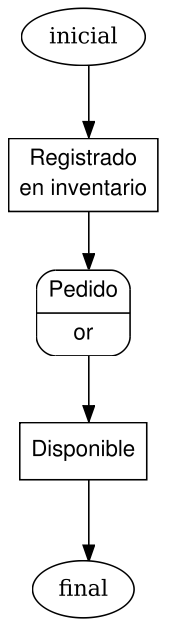
\includegraphics{grafo_inflow3.png}
\caption{\textbf{Figura 31: Disponible}}\label{_templates/Contenido6/Parte4:figura31}\end{figure}
\end{quote}

Descripción de la {\hyperref[_templates/Contenido6/Parte4:figura31]{\emph{Figura 31: Disponible}}}:
\begin{itemize}
\item {} 
La condición del circulo \textbf{inicial} apunta a la primera tarea de cuadro \textbf{Registrado}.

\item {} 
La primera tarea \textbf{Registrado} apunta a la segunda tarea \textbf{Pedido}.

\item {} 
La segunda tarea apunta a 2 tareas la primera opción de tarea es la del cuadro \textbf{Disponible}

\item {} 
La primera opción de tarea apunta a la condición de circulo \textbf{final}

\item {} 
En esta imagen vemos como se conectan la condición  \textbf{inicial} con la primera tarea \textbf{Registrado}, la tarea primera tarea con la segunda tarea \textbf{Pedido}, la segunda tarea apunta a dos opciones de tareas la cual la primera opción es la tarea \textbf{Disponible} y la primera opción de tarea apunta a la condición \textbf{final}.

\end{itemize}
\end{notice}
\end{quote}
\end{quote}


\subsection{\textbf{5.4 - CUARTA TAREA (Por\_llegar)}}
\label{_templates/Contenido6/Parte4:cuarta-tarea-por-llegar}\begin{quote}

En la cuarta tarea \textbf{(Por\_llegar)} se utilizaran las siguientes \textbf{etiquetas (XML)}:
\begin{itemize}
\item {} 
\textbf{\textless{}connection\textgreater{}}: \textbf{Por\_llegar} apunta a \textbf{final}, esto varia.

\item {} 
\textbf{\textless{}task\textgreater{}:} Nombre de la tarea \textbf{(Por\_llegar)}.

\item {} 
\textbf{\textless{}port\textgreater{}}:  \textbf{Por\_llegar} apunta a una opción.

\item {} 
\textbf{\textless{}variable\textgreater{}:} Variable \textbf{vPor\_llegar} donde nos aparecerá \textbf{(nombre,id,status,fecha y hora)} de esa acción.

\end{itemize}

Abrimos el archivo \textbf{productos.xml} y insertamos el código \textbf{(xml)} de la \textbf{tarea Por\_llegar} que aparece en el siguiente block:
\begin{quote}

\begin{notice}{note}{Nota:}
En la tarea \textbf{Pedido} se agrega otra etiqueta \textbf{\textless{}connection\textgreater{}} que seria segunda opción de tarea.
\end{notice}
\end{quote}

\begin{Verbatim}[commandchars=\\\{\}]
\PYG{c}{\PYGZlt{}!\PYGZhy{}\PYGZhy{}}
\PYG{c}{*********************}
\PYG{c}{\textbar{} Condición inicial \textbar{}}
\PYG{c}{*********************}
\PYG{c}{\PYGZhy{}\PYGZhy{}\PYGZgt{}}
  \PYG{n+nt}{\PYGZlt{}condition} \PYG{n+na}{type=}\PYG{l+s}{\PYGZdq{}start\PYGZdq{}} \PYG{n+na}{id=}\PYG{l+s}{\PYGZdq{}inicial\PYGZdq{}}\PYG{n+nt}{\PYGZgt{}}
   \PYG{n+nt}{\PYGZlt{}port} \PYG{n+na}{side=}\PYG{l+s}{\PYGZdq{}forward\PYGZdq{}} \PYG{n+na}{type=}\PYG{l+s}{\PYGZdq{}split\PYGZdq{}}\PYG{n+nt}{\PYGZgt{}}
    \PYG{n+nt}{\PYGZlt{}connection} \PYG{n+na}{query=}\PYG{l+s}{\PYGZdq{}select status from productos\PYGZdq{}} \PYG{n+na}{options=}\PYG{l+s}{\PYGZdq{}Registrado\PYGZdq{}} \PYG{n+na}{source=}\PYG{l+s}{\PYGZdq{}Registrado\PYGZdq{}}\PYG{n+nt}{/\PYGZgt{}}
   \PYG{n+nt}{\PYGZlt{}/port\PYGZgt{}}
  \PYG{n+nt}{\PYGZlt{}/condition\PYGZgt{}}


  \PYG{c}{\PYGZlt{}!\PYGZhy{}\PYGZhy{}}
\PYG{c}{  **************}
\PYG{c}{  \textbar{} Registrado \textbar{}}
\PYG{c}{  **************}
\PYG{c}{  }\PYG{c}{\PYGZhy{}\PYGZhy{}\PYGZgt{}}
  \PYG{n+nt}{\PYGZlt{}task} \PYG{n+na}{title=}\PYG{l+s}{\PYGZdq{}en inventario\PYGZdq{}} \PYG{n+na}{id=}\PYG{l+s}{\PYGZdq{}Registrado\PYGZdq{}}\PYG{n+nt}{\PYGZgt{}}
   \PYG{n+nt}{\PYGZlt{}port} \PYG{n+na}{side=}\PYG{l+s}{\PYGZdq{}forward\PYGZdq{}} \PYG{n+na}{type=}\PYG{l+s}{\PYGZdq{}split\PYGZdq{}}\PYG{n+nt}{\PYGZgt{}}
    \PYG{n+nt}{\PYGZlt{}connection} \PYG{n+na}{query=}\PYG{l+s}{\PYGZdq{}select status from productos\PYGZdq{}} \PYG{n+na}{options=}\PYG{l+s}{\PYGZdq{}Pedido\PYGZdq{}} \PYG{n+na}{source=}\PYG{l+s}{\PYGZdq{}Pedido\PYGZdq{}}\PYG{n+nt}{/\PYGZgt{}}
   \PYG{n+nt}{\PYGZlt{}/port\PYGZgt{}}
   \PYG{n+nt}{\PYGZlt{}variable} \PYG{n+na}{config=}\PYG{l+s}{\PYGZdq{}1\PYGZdq{}} \PYG{n+na}{documentsource=}\PYG{l+s}{\PYGZdq{}select id,nombre,status from productos\PYGZdq{}} \PYG{n+na}{type=}\PYG{l+s}{\PYGZdq{}sql\PYGZdq{}} \PYG{n+na}{tokenlink=}\PYG{l+s}{\PYGZdq{}\PYGZdq{}}
    \PYG{n+na}{id=}\PYG{l+s}{\PYGZdq{}vRegistrado\PYGZdq{}} \PYG{n+na}{rolfield=}\PYG{l+s}{\PYGZdq{}(select rol from productos\PYGZus{}registro}
\PYG{l+s}{    where productoid=productos.id and regstatus=\PYGZsq{}Registrado\PYGZsq{}) as rol\PYGZdq{}} \PYG{n+na}{scope=}\PYG{l+s}{\PYGZdq{}task\PYGZdq{}}
    \PYG{n+na}{timestampfield=}\PYG{l+s}{\PYGZdq{}(select fecha from productos\PYGZus{}registro}
\PYG{l+s}{    where productoid=productos.id and regstatus=\PYGZsq{}Registrado\PYGZsq{}) as fecha\PYGZdq{}}\PYG{n+nt}{/\PYGZgt{}}
  \PYG{n+nt}{\PYGZlt{}/task\PYGZgt{}}


  \PYG{c}{\PYGZlt{}!\PYGZhy{}\PYGZhy{}}
\PYG{c}{  **********}
\PYG{c}{  \textbar{} Pedido \textbar{}}
\PYG{c}{  **********}
\PYG{c}{  }\PYG{c}{\PYGZhy{}\PYGZhy{}\PYGZgt{}}
  \PYG{n+nt}{\PYGZlt{}task} \PYG{n+na}{title=}\PYG{l+s}{\PYGZdq{}\PYGZdq{}} \PYG{n+na}{id=}\PYG{l+s}{\PYGZdq{}Pedido\PYGZdq{}} \PYG{n+na}{textualinfo=}\PYG{l+s}{\PYGZdq{}\PYGZdq{}}\PYG{n+nt}{\PYGZgt{}}
   \PYG{n+nt}{\PYGZlt{}port} \PYG{n+na}{pattern=}\PYG{l+s}{\PYGZdq{}or\PYGZdq{}} \PYG{n+na}{side=}\PYG{l+s}{\PYGZdq{}forward\PYGZdq{}} \PYG{n+na}{type=}\PYG{l+s}{\PYGZdq{}split\PYGZdq{}}\PYG{n+nt}{\PYGZgt{}}
    \PYG{n+nt}{\PYGZlt{}connection} \PYG{n+na}{query=}\PYG{l+s}{\PYGZdq{}select status from productos\PYGZdq{}} \PYG{n+na}{options=}\PYG{l+s}{\PYGZdq{}Disponible\PYGZdq{}} \PYG{n+na}{source=}\PYG{l+s}{\PYGZdq{}Disponible\PYGZdq{}}\PYG{n+nt}{/\PYGZgt{}}
    \PYG{n+nt}{\PYGZlt{}connection} \PYG{n+na}{query=}\PYG{l+s}{\PYGZdq{}select status from productos\PYGZdq{}} \PYG{n+na}{options=}\PYG{l+s}{\PYGZdq{}Por\PYGZus{}llegar\PYGZdq{}} \PYG{n+na}{source=}\PYG{l+s}{\PYGZdq{}Por\PYGZus{}llegar\PYGZdq{}}\PYG{n+nt}{/\PYGZgt{}}
   \PYG{n+nt}{\PYGZlt{}/port\PYGZgt{}}
   \PYG{n+nt}{\PYGZlt{}variable} \PYG{n+na}{config=}\PYG{l+s}{\PYGZdq{}1\PYGZdq{}} \PYG{n+na}{documentsource=}\PYG{l+s}{\PYGZdq{}select id,nombre,status from productos\PYGZdq{}} \PYG{n+na}{type=}\PYG{l+s}{\PYGZdq{}sql\PYGZdq{}} \PYG{n+na}{tokenlink=}\PYG{l+s}{\PYGZdq{}\PYGZdq{}}
    \PYG{n+na}{id=}\PYG{l+s}{\PYGZdq{}vPedido\PYGZdq{}} \PYG{n+na}{rolfield=}\PYG{l+s}{\PYGZdq{}(select rol from\PYGZam{}\PYGZsh{}xa;productos\PYGZus{}registro}
\PYG{l+s}{    where productoid=productos.id and regstatus=\PYGZsq{}Pedido\PYGZsq{}) as rol\PYGZdq{}} \PYG{n+na}{scope=}\PYG{l+s}{\PYGZdq{}task\PYGZdq{}}
    \PYG{n+na}{timestampfield=}\PYG{l+s}{\PYGZdq{}(select fecha from productos\PYGZus{}registro}
\PYG{l+s}{    where productoid=productos.id and regstatus=\PYGZsq{}Pedido\PYGZsq{}) as fecha\PYGZdq{}}\PYG{n+nt}{/\PYGZgt{}}
  \PYG{n+nt}{\PYGZlt{}/task\PYGZgt{}}

  \PYG{c}{\PYGZlt{}!\PYGZhy{}\PYGZhy{}}
\PYG{c}{  **************}
\PYG{c}{  \textbar{} Disponible \textbar{}}
\PYG{c}{  **************}
\PYG{c}{  }\PYG{c}{\PYGZhy{}\PYGZhy{}\PYGZgt{}}
  \PYG{n+nt}{\PYGZlt{}task} \PYG{n+na}{title=}\PYG{l+s}{\PYGZdq{}\PYGZdq{}} \PYG{n+na}{id=}\PYG{l+s}{\PYGZdq{}Disponible\PYGZdq{}} \PYG{n+na}{textualinfo=}\PYG{l+s}{\PYGZdq{}\PYGZdq{}}\PYG{n+nt}{\PYGZgt{}}
   \PYG{n+nt}{\PYGZlt{}port} \PYG{n+na}{pattern=}\PYG{l+s}{\PYGZdq{}none\PYGZdq{}} \PYG{n+na}{side=}\PYG{l+s}{\PYGZdq{}forward\PYGZdq{}} \PYG{n+na}{type=}\PYG{l+s}{\PYGZdq{}split\PYGZdq{}}\PYG{n+nt}{\PYGZgt{}}
    \PYG{n+nt}{\PYGZlt{}connection} \PYG{n+na}{query=}\PYG{l+s}{\PYGZdq{}true\PYGZdq{}} \PYG{n+na}{options=}\PYG{l+s}{\PYGZdq{}\PYGZdq{}} \PYG{n+na}{source=}\PYG{l+s}{\PYGZdq{}final\PYGZdq{}}\PYG{n+nt}{/\PYGZgt{}}
   \PYG{n+nt}{\PYGZlt{}/port\PYGZgt{}}
   \PYG{n+nt}{\PYGZlt{}variable} \PYG{n+na}{config=}\PYG{l+s}{\PYGZdq{}1\PYGZdq{}} \PYG{n+na}{documentsource=}\PYG{l+s}{\PYGZdq{}select id,nombre,status from productos\PYGZdq{}} \PYG{n+na}{type=}\PYG{l+s}{\PYGZdq{}sql\PYGZdq{}} \PYG{n+na}{tokenlink=}\PYG{l+s}{\PYGZdq{}\PYGZdq{}}
    \PYG{n+na}{id=}\PYG{l+s}{\PYGZdq{}vDisponible\PYGZdq{}} \PYG{n+na}{rolfield=}\PYG{l+s}{\PYGZdq{}(select rol from\PYGZam{}\PYGZsh{}xa;productos\PYGZus{}registro}
\PYG{l+s}{    where productoid=productos.id and regstatus=\PYGZsq{}Disponible\PYGZsq{}) as rol\PYGZdq{}} \PYG{n+na}{scope=}\PYG{l+s}{\PYGZdq{}task\PYGZdq{}}
    \PYG{n+na}{timestampfield=}\PYG{l+s}{\PYGZdq{}(select fecha from productos\PYGZus{}registro}
\PYG{l+s}{    where productoid=productos.id and regstatus=\PYGZsq{}Disponible\PYGZsq{}) as fecha\PYGZdq{}}\PYG{n+nt}{/\PYGZgt{}}
  \PYG{n+nt}{\PYGZlt{}/task\PYGZgt{}}


  \PYG{c}{\PYGZlt{}!\PYGZhy{}\PYGZhy{}}
\PYG{c}{  **************}
\PYG{c}{  \textbar{} Por\PYGZus{}llegar \textbar{}}
\PYG{c}{  **************}
\PYG{c}{  }\PYG{c}{\PYGZhy{}\PYGZhy{}\PYGZgt{}}
  \PYG{n+nt}{\PYGZlt{}task} \PYG{n+na}{title=}\PYG{l+s}{\PYGZdq{}\PYGZdq{}} \PYG{n+na}{id=}\PYG{l+s}{\PYGZdq{}Por\PYGZus{}llegar\PYGZdq{}} \PYG{n+na}{textualinfo=}\PYG{l+s}{\PYGZdq{}\PYGZdq{}}\PYG{n+nt}{\PYGZgt{}}
   \PYG{n+nt}{\PYGZlt{}port} \PYG{n+na}{pattern=}\PYG{l+s}{\PYGZdq{}none\PYGZdq{}} \PYG{n+na}{side=}\PYG{l+s}{\PYGZdq{}forward\PYGZdq{}} \PYG{n+na}{type=}\PYG{l+s}{\PYGZdq{}split\PYGZdq{}}\PYG{n+nt}{\PYGZgt{}}
    \PYG{n+nt}{\PYGZlt{}connection} \PYG{n+na}{query=}\PYG{l+s}{\PYGZdq{}true\PYGZdq{}} \PYG{n+na}{options=}\PYG{l+s}{\PYGZdq{}\PYGZdq{}} \PYG{n+na}{source=}\PYG{l+s}{\PYGZdq{}final\PYGZdq{}}\PYG{n+nt}{/\PYGZgt{}}
   \PYG{n+nt}{\PYGZlt{}/port\PYGZgt{}}
   \PYG{n+nt}{\PYGZlt{}variable} \PYG{n+na}{config=}\PYG{l+s}{\PYGZdq{}1\PYGZdq{}} \PYG{n+na}{documentsource=}\PYG{l+s}{\PYGZdq{}select id,nombre,status from productos\PYGZdq{}} \PYG{n+na}{type=}\PYG{l+s}{\PYGZdq{}sql\PYGZdq{}} \PYG{n+na}{tokenlink=}\PYG{l+s}{\PYGZdq{}\PYGZdq{}}
    \PYG{n+na}{id=}\PYG{l+s}{\PYGZdq{}vPor\PYGZus{}llegar\PYGZdq{}} \PYG{n+na}{rolfield=}\PYG{l+s}{\PYGZdq{}(select rol from\PYGZam{}\PYGZsh{}xa;productos\PYGZus{}registro}
\PYG{l+s}{    where productoid=productos.id and regstatus=\PYGZsq{}Por\PYGZus{}llegar\PYGZsq{}) as rol\PYGZdq{}} \PYG{n+na}{scope=}\PYG{l+s}{\PYGZdq{}task\PYGZdq{}}
    \PYG{n+na}{timestampfield=}\PYG{l+s}{\PYGZdq{}(select fecha from productos\PYGZus{}registro}
\PYG{l+s}{    where productoid=productos.id and regstatus=\PYGZsq{}Por\PYGZus{}llegar\PYGZsq{}) as fecha\PYGZdq{}}\PYG{n+nt}{/\PYGZgt{}}
  \PYG{n+nt}{\PYGZlt{}/task\PYGZgt{}}



\PYG{c}{\PYGZlt{}!\PYGZhy{}\PYGZhy{}}
\PYG{c}{*******************}
\PYG{c}{\textbar{} Condición final \textbar{}}
\PYG{c}{*******************}
\PYG{c}{\PYGZhy{}\PYGZhy{}\PYGZgt{}}
  \PYG{n+nt}{\PYGZlt{}condition} \PYG{n+na}{id=}\PYG{l+s}{\PYGZdq{}final\PYGZdq{}}\PYG{n+nt}{\PYGZgt{}}
   \PYG{n+nt}{\PYGZlt{}port} \PYG{n+na}{side=}\PYG{l+s}{\PYGZdq{}forward\PYGZdq{}} \PYG{n+na}{type=}\PYG{l+s}{\PYGZdq{}split\PYGZdq{}}\PYG{n+nt}{\PYGZgt{}}
    \PYG{n+nt}{\PYGZlt{}connection} \PYG{n+na}{source=}\PYG{l+s}{\PYGZdq{}\PYGZdq{}}\PYG{n+nt}{/\PYGZgt{}}
   \PYG{n+nt}{\PYGZlt{}/port\PYGZgt{}}
  \PYG{n+nt}{\PYGZlt{}/condition\PYGZgt{}}
\end{Verbatim}

\textbf{Ahora ejecutaremos los siguiente pasos:}

\begin{notice}{note}{Nota:}
En el {\hyperref[_templates/Contenido6/Parte4:cuartopaso]{\emph{4° CUARTO PASO}}} creamos la carpeta llamada \textbf{tmp} y el archivo llamado \textbf{.py (Script\_graficos.py)} ,la cual se utilizaran en este paso a seguir.
\end{notice}
\begin{itemize}
\item {} 
Ejecutamos el mismo archivo \textbf{.py (Script\_graficos.py)} con el mismo contenido, desde la consola de comando como usuario normal.

\end{itemize}
\begin{quote}

\begin{Verbatim}[commandchars=\\\{\}]
\PYG{n+nv}{\PYGZdl{} }python \PYG{n+nv}{\PYGZdl{}HOME}/Script\PYGZus{}graficos.py
\end{Verbatim}

\begin{notice}{note}{Nota:}
Al ejecutar el archivo \textbf{.py (Script\_graficos.py)} nos mostrara un mensaje donde salen reflejadas las 2 \textbf{Condiciones principales} y la 4 tarea \textbf{(Registrado),(Pedido),(Disponible {[}OR{]} Por\_llegar)}:
\begin{quote}

\begin{Verbatim}[commandchars=\\\{\}]
QFSFileEngine::open: No file name specified
QSqlDatabasePrivate::removeDatabase: connection \PYG{l+s+s1}{\PYGZsq{}/home/cenditel/.safet/mydb.db\PYGZsq{}}
is still in use, all queries will cease to work.
.............wheretokens: on
.......newnode: \textbar{}Disponible\textbar{} \PYG{c}{\PYGZsh{} Tarea (Primera opción) Disponible}
.......newnode: \textbar{}Pedido\textbar{}     \PYG{c}{\PYGZsh{} Tarea Pedido}
.......newnode: \textbar{}Por\PYGZus{}llegar\textbar{} \PYG{c}{\PYGZsh{} Nueva tarea (Segunda opción) Por\PYGZus{}llegar}
.......newnode: \textbar{}Registrado\textbar{} \PYG{c}{\PYGZsh{} Tarea Registrado}
.......newnode: \textbar{}inicial\textbar{}    \PYG{c}{\PYGZsh{} Condición inicial}
.......newnode: \textbar{}final\textbar{}      \PYG{c}{\PYGZsh{} Condición final}
qt\PYGZus{}temp.XM6368.svg           \PYG{c}{\PYGZsh{} Obtenemos la nueva imagen con su nombre la cual contiene el gráfico}
\end{Verbatim}
\end{quote}

\textbf{El nombre de la imagen (.svg) es temporal, es decir su nombre varia constante mente.}
\end{notice}

\begin{notice}{note}{Nota:}
El nombre de la imagen (.svg) es temporal, es decir su nombre varia constante mente.
\end{notice}
\end{quote}
\begin{itemize}
\item {} 
Nos vamos al directorio \textbf{\$HOME/tmp},desde la consola de comando.

\end{itemize}
\begin{quote}

\begin{Verbatim}[commandchars=\\\{\}]
\PYG{n+nv}{\PYGZdl{} }\PYG{n+nb}{cd} \PYG{n+nv}{\PYGZdl{}HOME}/tmp
\end{Verbatim}
\end{quote}
\begin{itemize}
\item {} 
Escribimos el comando \textbf{ls} para ver las 5 imágenes \textbf{.svg} que hemos obtenido ,desde la consola de comando.

\end{itemize}
\begin{quote}

\begin{Verbatim}[commandchars=\\\{\}]
tmp\PYG{n+nv}{\PYGZdl{} }ls
qt\PYGZus{}temp.XM6827.svg, qt\PYGZus{}temp.XM6970.svg, qt\PYGZus{}temp.XM5792.svg, qt\PYGZus{}temp.XM6088.svg, qt\PYGZus{}temp.XM6368.svg
\end{Verbatim}
\end{quote}
\begin{itemize}
\item {} 
Con el comando \textbf{eog} vemos la tercera imagen \textbf{.svg(qt\_temp.XM6368.svg)} ,desde la consola de comando.

\end{itemize}
\begin{quote}

\begin{Verbatim}[commandchars=\\\{\}]
tmp\PYG{n+nv}{\PYGZdl{} }eog qt\PYGZus{}temp.XM6368.svg
\end{Verbatim}

\begin{notice}{note}{Nota:}
Si realizó los pasos correctos, se mostrara el grafo como en la imagen siguiente {\hyperref[_templates/Contenido6/Parte4:figura32]{\emph{Figura 32: Por\_llegar}}}
\begin{quote}
\begin{figure}[htbp]
\centering
\capstart

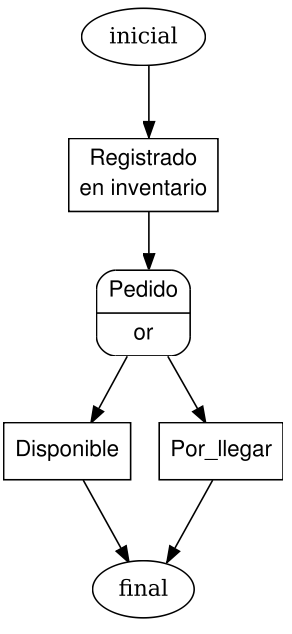
\includegraphics{grafo_inflow4.png}
\caption{\textbf{Figura 32: Por\_llegar}}\label{_templates/Contenido6/Parte4:figura32}\end{figure}
\end{quote}

Descripción de la {\hyperref[_templates/Contenido6/Parte4:figura32]{\emph{Figura 32: Por\_llegar}}}:
\begin{itemize}
\item {} 
La condición del circulo \textbf{inicial} apunta a la primera tarea de cuadro \textbf{Registrado}.

\item {} 
La primera tarea \textbf{Registrado} apunta a la segunda tarea \textbf{Pedido}.

\item {} 
La segunda tarea apunta a 2 tareas, la primera opción de tarea es la del cuadro \textbf{Disponible} y la segunda opción de tarea es la del cuadro \textbf{Por\_llegar}.

\item {} 
Las dos opción de tareas apunta a la condición de circulo \textbf{final}

\item {} 
En esta imagen vemos como se conectan la condición  \textbf{inicial} con la primera tarea \textbf{Registrado}, la tarea primera tarea con la segunda tarea \textbf{Pedido}, la segunda tarea apunta a dos opciones de tareas la cual la primera opción es la tarea \textbf{Disponible} y la segunda opción de tarea \textbf{Por\_llegar}, las dos opciones de tarea apuntan a la condición \textbf{final}.

\end{itemize}
\end{notice}
\end{quote}
\end{quote}


\subsection{\textbf{5.5 - QUINTA TAREA (Por\_agotarse)}}
\label{_templates/Contenido6/Parte4:quinta-tarea-por-agotarse}\begin{quote}

En la quinta tarea \textbf{(Por\_agotarse)} se utilizaran las siguientes \textbf{etiquetas (XML)}:
\begin{itemize}
\item {} 
\textbf{\textless{}connection\textgreater{}}: \textbf{Por\_agotarse} apunta a \textbf{final}, esto varia.

\item {} 
\textbf{\textless{}task\textgreater{}:} Nombre de la tarea \textbf{(Por\_agotarse)}.

\item {} 
\textbf{\textless{}port\textgreater{}}: \textbf{Por\_agotarse} apunta a una opción.

\item {} 
\textbf{\textless{}variable\textgreater{}:} Variable \textbf{vPor\_agotarse} donde nos aparecerá \textbf{(nombre,id,status,fecha y hora)} de esa acción.

\end{itemize}

Abrimos el archivo \textbf{productos.xml} y insertamos el código \textbf{(xml)} de la \textbf{tarea Por\_agotarse} que aparece en el siguiente block:
\begin{quote}

\begin{notice}{note}{Nota:}
En las opciones de tareas \textbf{Disponible y Por\_llegar} se modificará la etiqueta \textbf{\textless{}connection\textgreater{}} que apuntaran a la siguiente tarea \textbf{Por\_agotarse}.
\end{notice}
\end{quote}

\begin{Verbatim}[commandchars=\\\{\}]
\PYG{c}{\PYGZlt{}!\PYGZhy{}\PYGZhy{}}
\PYG{c}{*********************}
\PYG{c}{\textbar{} Condición inicial \textbar{}}
\PYG{c}{*********************}
\PYG{c}{\PYGZhy{}\PYGZhy{}\PYGZgt{}}
  \PYG{n+nt}{\PYGZlt{}condition} \PYG{n+na}{type=}\PYG{l+s}{\PYGZdq{}start\PYGZdq{}} \PYG{n+na}{id=}\PYG{l+s}{\PYGZdq{}inicial\PYGZdq{}}\PYG{n+nt}{\PYGZgt{}}
   \PYG{n+nt}{\PYGZlt{}port} \PYG{n+na}{side=}\PYG{l+s}{\PYGZdq{}forward\PYGZdq{}} \PYG{n+na}{type=}\PYG{l+s}{\PYGZdq{}split\PYGZdq{}}\PYG{n+nt}{\PYGZgt{}}
    \PYG{n+nt}{\PYGZlt{}connection} \PYG{n+na}{query=}\PYG{l+s}{\PYGZdq{}select status from productos\PYGZdq{}} \PYG{n+na}{options=}\PYG{l+s}{\PYGZdq{}Registrado\PYGZdq{}} \PYG{n+na}{source=}\PYG{l+s}{\PYGZdq{}Registrado\PYGZdq{}}\PYG{n+nt}{/\PYGZgt{}}
   \PYG{n+nt}{\PYGZlt{}/port\PYGZgt{}}
  \PYG{n+nt}{\PYGZlt{}/condition\PYGZgt{}}


  \PYG{c}{\PYGZlt{}!\PYGZhy{}\PYGZhy{}}
\PYG{c}{  **************}
\PYG{c}{  \textbar{} Registrado \textbar{}}
\PYG{c}{  **************}
\PYG{c}{  }\PYG{c}{\PYGZhy{}\PYGZhy{}\PYGZgt{}}
  \PYG{n+nt}{\PYGZlt{}task} \PYG{n+na}{title=}\PYG{l+s}{\PYGZdq{}en inventario\PYGZdq{}} \PYG{n+na}{id=}\PYG{l+s}{\PYGZdq{}Registrado\PYGZdq{}}\PYG{n+nt}{\PYGZgt{}}
   \PYG{n+nt}{\PYGZlt{}port} \PYG{n+na}{side=}\PYG{l+s}{\PYGZdq{}forward\PYGZdq{}} \PYG{n+na}{type=}\PYG{l+s}{\PYGZdq{}split\PYGZdq{}}\PYG{n+nt}{\PYGZgt{}}
    \PYG{n+nt}{\PYGZlt{}connection} \PYG{n+na}{query=}\PYG{l+s}{\PYGZdq{}select status from productos\PYGZdq{}} \PYG{n+na}{options=}\PYG{l+s}{\PYGZdq{}Pedido\PYGZdq{}} \PYG{n+na}{source=}\PYG{l+s}{\PYGZdq{}Pedido\PYGZdq{}}\PYG{n+nt}{/\PYGZgt{}}
   \PYG{n+nt}{\PYGZlt{}/port\PYGZgt{}}
   \PYG{n+nt}{\PYGZlt{}variable} \PYG{n+na}{config=}\PYG{l+s}{\PYGZdq{}1\PYGZdq{}} \PYG{n+na}{documentsource=}\PYG{l+s}{\PYGZdq{}select id,nombre,status from productos\PYGZdq{}} \PYG{n+na}{type=}\PYG{l+s}{\PYGZdq{}sql\PYGZdq{}} \PYG{n+na}{tokenlink=}\PYG{l+s}{\PYGZdq{}\PYGZdq{}}
    \PYG{n+na}{id=}\PYG{l+s}{\PYGZdq{}vRegistrado\PYGZdq{}} \PYG{n+na}{rolfield=}\PYG{l+s}{\PYGZdq{}(select rol from productos\PYGZus{}registro}
\PYG{l+s}{    where productoid=productos.id and regstatus=\PYGZsq{}Registrado\PYGZsq{}) as rol\PYGZdq{}} \PYG{n+na}{scope=}\PYG{l+s}{\PYGZdq{}task\PYGZdq{}}
    \PYG{n+na}{timestampfield=}\PYG{l+s}{\PYGZdq{}(select fecha from productos\PYGZus{}registro}
\PYG{l+s}{    where productoid=productos.id and regstatus=\PYGZsq{}Registrado\PYGZsq{}) as fecha\PYGZdq{}}\PYG{n+nt}{/\PYGZgt{}}
  \PYG{n+nt}{\PYGZlt{}/task\PYGZgt{}}


  \PYG{c}{\PYGZlt{}!\PYGZhy{}\PYGZhy{}}
\PYG{c}{  **********}
\PYG{c}{  \textbar{} Pedido \textbar{}}
\PYG{c}{  **********}
\PYG{c}{  }\PYG{c}{\PYGZhy{}\PYGZhy{}\PYGZgt{}}
  \PYG{n+nt}{\PYGZlt{}task} \PYG{n+na}{title=}\PYG{l+s}{\PYGZdq{}\PYGZdq{}} \PYG{n+na}{id=}\PYG{l+s}{\PYGZdq{}Pedido\PYGZdq{}} \PYG{n+na}{textualinfo=}\PYG{l+s}{\PYGZdq{}\PYGZdq{}}\PYG{n+nt}{\PYGZgt{}}
   \PYG{n+nt}{\PYGZlt{}port} \PYG{n+na}{pattern=}\PYG{l+s}{\PYGZdq{}or\PYGZdq{}} \PYG{n+na}{side=}\PYG{l+s}{\PYGZdq{}forward\PYGZdq{}} \PYG{n+na}{type=}\PYG{l+s}{\PYGZdq{}split\PYGZdq{}}\PYG{n+nt}{\PYGZgt{}}
    \PYG{n+nt}{\PYGZlt{}connection} \PYG{n+na}{query=}\PYG{l+s}{\PYGZdq{}select status from productos\PYGZdq{}} \PYG{n+na}{options=}\PYG{l+s}{\PYGZdq{}Disponible\PYGZdq{}} \PYG{n+na}{source=}\PYG{l+s}{\PYGZdq{}Disponible\PYGZdq{}}\PYG{n+nt}{/\PYGZgt{}}
    \PYG{n+nt}{\PYGZlt{}connection} \PYG{n+na}{query=}\PYG{l+s}{\PYGZdq{}select status from productos\PYGZdq{}} \PYG{n+na}{options=}\PYG{l+s}{\PYGZdq{}Por\PYGZus{}llegar\PYGZdq{}} \PYG{n+na}{source=}\PYG{l+s}{\PYGZdq{}Por\PYGZus{}llegar\PYGZdq{}}\PYG{n+nt}{/\PYGZgt{}}
   \PYG{n+nt}{\PYGZlt{}/port\PYGZgt{}}
   \PYG{n+nt}{\PYGZlt{}variable} \PYG{n+na}{config=}\PYG{l+s}{\PYGZdq{}1\PYGZdq{}} \PYG{n+na}{documentsource=}\PYG{l+s}{\PYGZdq{}select id,nombre,status from productos\PYGZdq{}} \PYG{n+na}{type=}\PYG{l+s}{\PYGZdq{}sql\PYGZdq{}} \PYG{n+na}{tokenlink=}\PYG{l+s}{\PYGZdq{}\PYGZdq{}}
    \PYG{n+na}{id=}\PYG{l+s}{\PYGZdq{}vPedido\PYGZdq{}} \PYG{n+na}{rolfield=}\PYG{l+s}{\PYGZdq{}(select rol from\PYGZam{}\PYGZsh{}xa;productos\PYGZus{}registro}
\PYG{l+s}{    where productoid=productos.id and regstatus=\PYGZsq{}Pedido\PYGZsq{}) as rol\PYGZdq{}} \PYG{n+na}{scope=}\PYG{l+s}{\PYGZdq{}task\PYGZdq{}}
    \PYG{n+na}{timestampfield=}\PYG{l+s}{\PYGZdq{}(select fecha from productos\PYGZus{}registro}
\PYG{l+s}{    where productoid=productos.id and regstatus=\PYGZsq{}Pedido\PYGZsq{}) as fecha\PYGZdq{}}\PYG{n+nt}{/\PYGZgt{}}
  \PYG{n+nt}{\PYGZlt{}/task\PYGZgt{}}

  \PYG{c}{\PYGZlt{}!\PYGZhy{}\PYGZhy{}}
\PYG{c}{  **************}
\PYG{c}{  \textbar{} Disponible \textbar{}}
\PYG{c}{  **************}
\PYG{c}{  }\PYG{c}{\PYGZhy{}\PYGZhy{}\PYGZgt{}}
  \PYG{n+nt}{\PYGZlt{}task} \PYG{n+na}{title=}\PYG{l+s}{\PYGZdq{}\PYGZdq{}} \PYG{n+na}{id=}\PYG{l+s}{\PYGZdq{}Disponible\PYGZdq{}} \PYG{n+na}{textualinfo=}\PYG{l+s}{\PYGZdq{}\PYGZdq{}}\PYG{n+nt}{\PYGZgt{}}
   \PYG{n+nt}{\PYGZlt{}port} \PYG{n+na}{pattern=}\PYG{l+s}{\PYGZdq{}none\PYGZdq{}} \PYG{n+na}{side=}\PYG{l+s}{\PYGZdq{}forward\PYGZdq{}} \PYG{n+na}{type=}\PYG{l+s}{\PYGZdq{}split\PYGZdq{}}\PYG{n+nt}{\PYGZgt{}}
    \PYG{n+nt}{\PYGZlt{}connection} \PYG{n+na}{query=}\PYG{l+s}{\PYGZdq{}select status from productos\PYGZdq{}} \PYG{n+na}{options=}\PYG{l+s}{\PYGZdq{}Por\PYGZus{}agotarse\PYGZdq{}} \PYG{n+na}{source=}\PYG{l+s}{\PYGZdq{}Por\PYGZus{}agotarse\PYGZdq{}}\PYG{n+nt}{/\PYGZgt{}}
   \PYG{n+nt}{\PYGZlt{}/port\PYGZgt{}}
   \PYG{n+nt}{\PYGZlt{}variable} \PYG{n+na}{config=}\PYG{l+s}{\PYGZdq{}1\PYGZdq{}} \PYG{n+na}{documentsource=}\PYG{l+s}{\PYGZdq{}select id,nombre,status from productos\PYGZdq{}} \PYG{n+na}{type=}\PYG{l+s}{\PYGZdq{}sql\PYGZdq{}} \PYG{n+na}{tokenlink=}\PYG{l+s}{\PYGZdq{}\PYGZdq{}}
    \PYG{n+na}{id=}\PYG{l+s}{\PYGZdq{}vDisponible\PYGZdq{}} \PYG{n+na}{rolfield=}\PYG{l+s}{\PYGZdq{}(select rol from\PYGZam{}\PYGZsh{}xa;productos\PYGZus{}registro}
\PYG{l+s}{    where productoid=productos.id and regstatus=\PYGZsq{}Disponible\PYGZsq{}) as rol\PYGZdq{}} \PYG{n+na}{scope=}\PYG{l+s}{\PYGZdq{}task\PYGZdq{}}
    \PYG{n+na}{timestampfield=}\PYG{l+s}{\PYGZdq{}(select fecha from productos\PYGZus{}registro}
\PYG{l+s}{    where productoid=productos.id and regstatus=\PYGZsq{}Disponible\PYGZsq{}) as fecha\PYGZdq{}}\PYG{n+nt}{/\PYGZgt{}}
  \PYG{n+nt}{\PYGZlt{}/task\PYGZgt{}}


  \PYG{c}{\PYGZlt{}!\PYGZhy{}\PYGZhy{}}
\PYG{c}{  **************}
\PYG{c}{  \textbar{} Por\PYGZus{}llegar \textbar{}}
\PYG{c}{  **************}
\PYG{c}{  }\PYG{c}{\PYGZhy{}\PYGZhy{}\PYGZgt{}}
  \PYG{n+nt}{\PYGZlt{}task} \PYG{n+na}{title=}\PYG{l+s}{\PYGZdq{}\PYGZdq{}} \PYG{n+na}{id=}\PYG{l+s}{\PYGZdq{}Por\PYGZus{}llegar\PYGZdq{}} \PYG{n+na}{textualinfo=}\PYG{l+s}{\PYGZdq{}\PYGZdq{}}\PYG{n+nt}{\PYGZgt{}}
   \PYG{n+nt}{\PYGZlt{}port} \PYG{n+na}{pattern=}\PYG{l+s}{\PYGZdq{}none\PYGZdq{}} \PYG{n+na}{side=}\PYG{l+s}{\PYGZdq{}forward\PYGZdq{}} \PYG{n+na}{type=}\PYG{l+s}{\PYGZdq{}split\PYGZdq{}}\PYG{n+nt}{\PYGZgt{}}
    \PYG{n+nt}{\PYGZlt{}connection} \PYG{n+na}{query=}\PYG{l+s}{\PYGZdq{}select status from productos\PYGZdq{}} \PYG{n+na}{options=}\PYG{l+s}{\PYGZdq{}Por\PYGZus{}agotarse\PYGZdq{}} \PYG{n+na}{source=}\PYG{l+s}{\PYGZdq{}Por\PYGZus{}agotarse\PYGZdq{}}\PYG{n+nt}{/\PYGZgt{}}
   \PYG{n+nt}{\PYGZlt{}/port\PYGZgt{}}
   \PYG{n+nt}{\PYGZlt{}variable} \PYG{n+na}{config=}\PYG{l+s}{\PYGZdq{}1\PYGZdq{}} \PYG{n+na}{documentsource=}\PYG{l+s}{\PYGZdq{}select id,nombre,status from productos\PYGZdq{}} \PYG{n+na}{type=}\PYG{l+s}{\PYGZdq{}sql\PYGZdq{}} \PYG{n+na}{tokenlink=}\PYG{l+s}{\PYGZdq{}\PYGZdq{}}
    \PYG{n+na}{id=}\PYG{l+s}{\PYGZdq{}vPor\PYGZus{}llegar\PYGZdq{}} \PYG{n+na}{rolfield=}\PYG{l+s}{\PYGZdq{}(select rol from\PYGZam{}\PYGZsh{}xa;productos\PYGZus{}registro}
\PYG{l+s}{    where productoid=productos.id and regstatus=\PYGZsq{}Por\PYGZus{}llegar\PYGZsq{}) as rol\PYGZdq{}} \PYG{n+na}{scope=}\PYG{l+s}{\PYGZdq{}task\PYGZdq{}}
    \PYG{n+na}{timestampfield=}\PYG{l+s}{\PYGZdq{}(select fecha from productos\PYGZus{}registro}
\PYG{l+s}{    where productoid=productos.id and regstatus=\PYGZsq{}Por\PYGZus{}llegar\PYGZsq{}) as fecha\PYGZdq{}}\PYG{n+nt}{/\PYGZgt{}}
  \PYG{n+nt}{\PYGZlt{}/task\PYGZgt{}}



  \PYG{c}{\PYGZlt{}!\PYGZhy{}\PYGZhy{}}
\PYG{c}{  ****************}
\PYG{c}{  \textbar{} Por\PYGZus{}agotarse \textbar{}}
\PYG{c}{  ****************}
\PYG{c}{  }\PYG{c}{\PYGZhy{}\PYGZhy{}\PYGZgt{}}
  \PYG{n+nt}{\PYGZlt{}task} \PYG{n+na}{title=}\PYG{l+s}{\PYGZdq{}\PYGZdq{}} \PYG{n+na}{id=}\PYG{l+s}{\PYGZdq{}Por\PYGZus{}agotarse\PYGZdq{}} \PYG{n+na}{textualinfo=}\PYG{l+s}{\PYGZdq{}\PYGZdq{}}\PYG{n+nt}{\PYGZgt{}}
   \PYG{n+nt}{\PYGZlt{}port} \PYG{n+na}{pattern=}\PYG{l+s}{\PYGZdq{}none\PYGZdq{}} \PYG{n+na}{side=}\PYG{l+s}{\PYGZdq{}forward\PYGZdq{}} \PYG{n+na}{type=}\PYG{l+s}{\PYGZdq{}split\PYGZdq{}}\PYG{n+nt}{\PYGZgt{}}
    \PYG{n+nt}{\PYGZlt{}connection} \PYG{n+na}{query=}\PYG{l+s}{\PYGZdq{}true\PYGZdq{}} \PYG{n+na}{options=}\PYG{l+s}{\PYGZdq{}\PYGZdq{}} \PYG{n+na}{source=}\PYG{l+s}{\PYGZdq{}final\PYGZdq{}}\PYG{n+nt}{/\PYGZgt{}}
   \PYG{n+nt}{\PYGZlt{}/port\PYGZgt{}}
   \PYG{n+nt}{\PYGZlt{}variable} \PYG{n+na}{config=}\PYG{l+s}{\PYGZdq{}1\PYGZdq{}} \PYG{n+na}{documentsource=}\PYG{l+s}{\PYGZdq{}select id,nombre,status from productos\PYGZdq{}} \PYG{n+na}{type=}\PYG{l+s}{\PYGZdq{}sql\PYGZdq{}} \PYG{n+na}{tokenlink=}\PYG{l+s}{\PYGZdq{}\PYGZdq{}}
    \PYG{n+na}{id=}\PYG{l+s}{\PYGZdq{}vPor\PYGZus{}agotarse\PYGZdq{}} \PYG{n+na}{rolfield=}\PYG{l+s}{\PYGZdq{}(select rol from\PYGZam{}\PYGZsh{}xa;productos\PYGZus{}registro}
\PYG{l+s}{    where productoid=productos.id and regstatus=\PYGZsq{}Por\PYGZus{}agotarse\PYGZsq{}) as rol\PYGZdq{}} \PYG{n+na}{scope=}\PYG{l+s}{\PYGZdq{}task\PYGZdq{}}
    \PYG{n+na}{timestampfield=}\PYG{l+s}{\PYGZdq{}(select fecha from productos\PYGZus{}registro}
\PYG{l+s}{    where productoid=productos.id and regstatus=\PYGZsq{}Por\PYGZus{}agotarse\PYGZsq{}) as fecha\PYGZdq{}}\PYG{n+nt}{/\PYGZgt{}}
  \PYG{n+nt}{\PYGZlt{}/task\PYGZgt{}}

\PYG{c}{\PYGZlt{}!\PYGZhy{}\PYGZhy{}}
\PYG{c}{*******************}
\PYG{c}{\textbar{} Condición final \textbar{}}
\PYG{c}{*******************}
\PYG{c}{\PYGZhy{}\PYGZhy{}\PYGZgt{}}
  \PYG{n+nt}{\PYGZlt{}condition} \PYG{n+na}{id=}\PYG{l+s}{\PYGZdq{}final\PYGZdq{}}\PYG{n+nt}{\PYGZgt{}}
   \PYG{n+nt}{\PYGZlt{}port} \PYG{n+na}{side=}\PYG{l+s}{\PYGZdq{}forward\PYGZdq{}} \PYG{n+na}{type=}\PYG{l+s}{\PYGZdq{}split\PYGZdq{}}\PYG{n+nt}{\PYGZgt{}}
    \PYG{n+nt}{\PYGZlt{}connection} \PYG{n+na}{source=}\PYG{l+s}{\PYGZdq{}\PYGZdq{}}\PYG{n+nt}{/\PYGZgt{}}
   \PYG{n+nt}{\PYGZlt{}/port\PYGZgt{}}
  \PYG{n+nt}{\PYGZlt{}/condition\PYGZgt{}}
\end{Verbatim}

\textbf{Ahora ejecutaremos los siguiente pasos:}

\begin{notice}{note}{Nota:}
En el {\hyperref[_templates/Contenido6/Parte4:cuartopaso]{\emph{4° CUARTO PASO}}} creamos la carpeta llamada \textbf{tmp} y el archivo llamado \textbf{.py (Script\_graficos.py)} ,la cual se utilizaran en este paso a seguir.
\end{notice}
\begin{itemize}
\item {} 
Ejecutamos el mismo archivo \textbf{.py (Script\_graficos.py)} con el mismo contenido, desde la consola de comando como usuario normal.

\end{itemize}
\begin{quote}

\begin{Verbatim}[commandchars=\\\{\}]
\PYG{n+nv}{\PYGZdl{} }python \PYG{n+nv}{\PYGZdl{}HOME}/Script\PYGZus{}graficos.py
\end{Verbatim}

\begin{notice}{note}{Nota:}
Al ejecutar el archivo \textbf{.py (Script\_graficos.py)} nos mostrara un mensaje donde salen reflejadas las 2 \textbf{Condiciones principales} y la 4 tarea \textbf{(Registrado),(Pedido),(Disponible {[}OR{]} Por\_llegar)}:
\begin{quote}

\begin{Verbatim}[commandchars=\\\{\}]
QFSFileEngine::open: No file name specified
QSqlDatabasePrivate::removeDatabase: connection \PYG{l+s+s1}{\PYGZsq{}/home/cenditel/.safet/mydb.db\PYGZsq{}}
is still in use, all queries will cease to work.
.............wheretokens: on
.......newnode: \textbar{}Disponible\textbar{}   \PYG{c}{\PYGZsh{} Tarea (Primera opción) Disponible}
.......newnode: \textbar{}Pedido\textbar{}       \PYG{c}{\PYGZsh{} Tarea Pedido}
.......newnode: \textbar{}Por\PYGZus{}agotarse\textbar{} \PYG{c}{\PYGZsh{} Nueva tarea Por\PYGZus{}agotarse}
.......newnode: \textbar{}Por\PYGZus{}llegar\textbar{}   \PYG{c}{\PYGZsh{} Tarea (Segunda opción) Por\PYGZus{}llegar}
.......newnode: \textbar{}Registrado\textbar{}   \PYG{c}{\PYGZsh{} Tarea Registrado}
.......newnode: \textbar{}inicial\textbar{}      \PYG{c}{\PYGZsh{} Condición inicial}
.......newnode: \textbar{}final\textbar{}        \PYG{c}{\PYGZsh{} Condición final}
qt\PYGZus{}temp.XM6667.svg             \PYG{c}{\PYGZsh{} Obtenemos la nueva imagen con su nombre la cual contiene el gráfico}
\end{Verbatim}
\end{quote}

\textbf{El nombre de la imagen (.svg) es temporal, es decir su nombre varia constante mente.}
\end{notice}

\begin{notice}{note}{Nota:}
El nombre de la imagen (.svg) es temporal, es decir su nombre varia constante mente.
\end{notice}
\end{quote}
\begin{itemize}
\item {} 
Nos vamos al directorio \textbf{\$HOME/tmp},desde la consola de comando.

\end{itemize}
\begin{quote}

\begin{Verbatim}[commandchars=\\\{\}]
\PYG{n+nv}{\PYGZdl{} }\PYG{n+nb}{cd} \PYG{n+nv}{\PYGZdl{}HOME}/tmp
\end{Verbatim}
\end{quote}
\begin{itemize}
\item {} 
Escribimos el comando \textbf{ls} para ver las 5 imágenes \textbf{.svg} que hemos obtenido ,desde la consola de comando.

\end{itemize}
\begin{quote}

\begin{Verbatim}[commandchars=\\\{\}]
tmp\PYG{n+nv}{\PYGZdl{} }ls
qt\PYGZus{}temp.XM6827.svg, qt\PYGZus{}temp.XM6970.svg, qt\PYGZus{}temp.XM5792.svg, qt\PYGZus{}temp.XM6088.svg,
qt\PYGZus{}temp.XM6368.svg, qt\PYGZus{}temp.XM6667.svg
\end{Verbatim}
\end{quote}
\begin{itemize}
\item {} 
Con el comando \textbf{eog} vemos la tercera imagen \textbf{.svg(qt\_temp.XM6667.svg)} ,desde la consola de comando.

\end{itemize}
\begin{quote}

\begin{Verbatim}[commandchars=\\\{\}]
tmp\PYG{n+nv}{\PYGZdl{} }eog qt\PYGZus{}temp.XM6667.svg
\end{Verbatim}

\begin{notice}{note}{Nota:}
Si realizó los pasos correctos, se mostrara el grafo como en la imagen siguiente {\hyperref[_templates/Contenido6/Parte4:figura33]{\emph{Figura 33: Por\_agotarse}}}
\begin{quote}
\begin{figure}[htbp]
\centering
\capstart

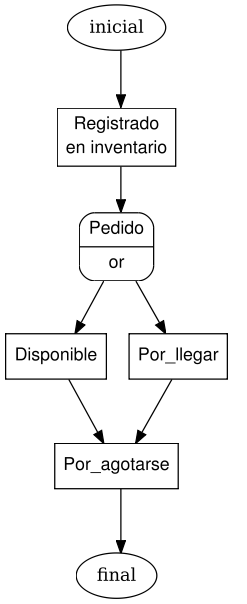
\includegraphics{grafo_inflow6.png}
\caption{\textbf{Figura 33: Por\_agotarse}}\label{_templates/Contenido6/Parte4:figura33}\end{figure}
\end{quote}

Descripción de la {\hyperref[_templates/Contenido6/Parte4:figura33]{\emph{Figura 33: Por\_agotarse}}}:
\begin{itemize}
\item {} 
La condición del circulo \textbf{inicial} apunta a la primera tarea de cuadro \textbf{Registrado}.

\item {} 
La primera tarea \textbf{Registrado} apunta a la segunda tarea \textbf{Pedido}.

\item {} 
La segunda tarea apunta a 2 tareas, la primera opción de tarea es la del cuadro \textbf{Disponible} y la segunda opción de tarea es la del cuadro \textbf{Por\_llegar}.

\item {} 
Las dos opción de tareas apunta a la quinta tarea del cuadro \textbf{Por\_agotarse}.

\item {} 
La quinta tarea apunta a la condición de circulo \textbf{final}

\item {} 
En esta imagen vemos como se conectan la condición  \textbf{inicial} con la primera tarea \textbf{Registrado}, la tarea primera tarea con la segunda tarea \textbf{Pedido}, la segunda tarea apunta a dos opciones de tareas la cual la primera opción es la tarea \textbf{Disponible} y la segunda opción de tarea \textbf{Por\_llegar}, las dos opciones de tarea apuntan a la quinta tarea \textbf{Por\_agotarse} y apunta a la condición \textbf{final}.

\end{itemize}
\end{notice}
\end{quote}
\end{quote}


\subsection{\textbf{5.6 - SEXTA TAREA (Agotado)}}
\label{_templates/Contenido6/Parte4:sexta-tarea-agotado}\begin{quote}

En la sexta tarea \textbf{(Agotado)} se utilizaran las siguientes \textbf{etiquetas (XML)}:
\begin{itemize}
\item {} 
\textbf{\textless{}connection\textgreater{}}: \textbf{Agotado} apunta a \textbf{(final, Pedido)},esto varia.

\item {} 
\textbf{\textless{}task\textgreater{}:} Nombre de la tarea \textbf{(Agotado)}.

\item {} 
\textbf{\textless{}port\textgreater{}}: \textbf{Agotado} apunta a dos opción.

\item {} 
\textbf{\textless{}variable\textgreater{}:} Variable \textbf{vAgotado} donde nos aparecerá \textbf{(nombre,id,status,fecha y hora)} de esa acción.

\end{itemize}

Abrimos el archivo \textbf{productos.xml} y insertamos el código \textbf{(xml)} de la tarea \textbf{Agotado} que aparece en el siguiente block:
\begin{quote}

\begin{notice}{note}{Nota:}
En la tarea \textbf{Por\_agotarse} se modificará la etiqueta \textbf{\textless{}connection\textgreater{}} que apuntaran a la siguiente tarea \textbf{Agotado}.
\end{notice}
\end{quote}

\begin{Verbatim}[commandchars=\\\{\}]
\PYG{c}{\PYGZlt{}!\PYGZhy{}\PYGZhy{}}
\PYG{c}{*********************}
\PYG{c}{\textbar{} Condición inicial \textbar{}}
\PYG{c}{*********************}
\PYG{c}{\PYGZhy{}\PYGZhy{}\PYGZgt{}}
  \PYG{n+nt}{\PYGZlt{}condition} \PYG{n+na}{type=}\PYG{l+s}{\PYGZdq{}start\PYGZdq{}} \PYG{n+na}{id=}\PYG{l+s}{\PYGZdq{}inicial\PYGZdq{}}\PYG{n+nt}{\PYGZgt{}}
   \PYG{n+nt}{\PYGZlt{}port} \PYG{n+na}{side=}\PYG{l+s}{\PYGZdq{}forward\PYGZdq{}} \PYG{n+na}{type=}\PYG{l+s}{\PYGZdq{}split\PYGZdq{}}\PYG{n+nt}{\PYGZgt{}}
    \PYG{n+nt}{\PYGZlt{}connection} \PYG{n+na}{query=}\PYG{l+s}{\PYGZdq{}select status from productos\PYGZdq{}} \PYG{n+na}{options=}\PYG{l+s}{\PYGZdq{}Registrado\PYGZdq{}} \PYG{n+na}{source=}\PYG{l+s}{\PYGZdq{}Registrado\PYGZdq{}}\PYG{n+nt}{/\PYGZgt{}}
   \PYG{n+nt}{\PYGZlt{}/port\PYGZgt{}}
  \PYG{n+nt}{\PYGZlt{}/condition\PYGZgt{}}


  \PYG{c}{\PYGZlt{}!\PYGZhy{}\PYGZhy{}}
\PYG{c}{  **************}
\PYG{c}{  \textbar{} Registrado \textbar{}}
\PYG{c}{  **************}
\PYG{c}{  }\PYG{c}{\PYGZhy{}\PYGZhy{}\PYGZgt{}}
  \PYG{n+nt}{\PYGZlt{}task} \PYG{n+na}{title=}\PYG{l+s}{\PYGZdq{}en inventario\PYGZdq{}} \PYG{n+na}{id=}\PYG{l+s}{\PYGZdq{}Registrado\PYGZdq{}}\PYG{n+nt}{\PYGZgt{}}
   \PYG{n+nt}{\PYGZlt{}port} \PYG{n+na}{side=}\PYG{l+s}{\PYGZdq{}forward\PYGZdq{}} \PYG{n+na}{type=}\PYG{l+s}{\PYGZdq{}split\PYGZdq{}}\PYG{n+nt}{\PYGZgt{}}
    \PYG{n+nt}{\PYGZlt{}connection} \PYG{n+na}{query=}\PYG{l+s}{\PYGZdq{}select status from productos\PYGZdq{}} \PYG{n+na}{options=}\PYG{l+s}{\PYGZdq{}Pedido\PYGZdq{}} \PYG{n+na}{source=}\PYG{l+s}{\PYGZdq{}Pedido\PYGZdq{}}\PYG{n+nt}{/\PYGZgt{}}
   \PYG{n+nt}{\PYGZlt{}/port\PYGZgt{}}
   \PYG{n+nt}{\PYGZlt{}variable} \PYG{n+na}{config=}\PYG{l+s}{\PYGZdq{}1\PYGZdq{}} \PYG{n+na}{documentsource=}\PYG{l+s}{\PYGZdq{}select id,nombre,status from productos\PYGZdq{}} \PYG{n+na}{type=}\PYG{l+s}{\PYGZdq{}sql\PYGZdq{}} \PYG{n+na}{tokenlink=}\PYG{l+s}{\PYGZdq{}\PYGZdq{}}
    \PYG{n+na}{id=}\PYG{l+s}{\PYGZdq{}vRegistrado\PYGZdq{}} \PYG{n+na}{rolfield=}\PYG{l+s}{\PYGZdq{}(select rol from productos\PYGZus{}registro}
\PYG{l+s}{    where productoid=productos.id and regstatus=\PYGZsq{}Registrado\PYGZsq{}) as rol\PYGZdq{}} \PYG{n+na}{scope=}\PYG{l+s}{\PYGZdq{}task\PYGZdq{}}
    \PYG{n+na}{timestampfield=}\PYG{l+s}{\PYGZdq{}(select fecha from productos\PYGZus{}registro}
\PYG{l+s}{    where productoid=productos.id and regstatus=\PYGZsq{}Registrado\PYGZsq{}) as fecha\PYGZdq{}}\PYG{n+nt}{/\PYGZgt{}}
  \PYG{n+nt}{\PYGZlt{}/task\PYGZgt{}}


  \PYG{c}{\PYGZlt{}!\PYGZhy{}\PYGZhy{}}
\PYG{c}{  **********}
\PYG{c}{  \textbar{} Pedido \textbar{}}
\PYG{c}{  **********}
\PYG{c}{  }\PYG{c}{\PYGZhy{}\PYGZhy{}\PYGZgt{}}
  \PYG{n+nt}{\PYGZlt{}task} \PYG{n+na}{title=}\PYG{l+s}{\PYGZdq{}\PYGZdq{}} \PYG{n+na}{id=}\PYG{l+s}{\PYGZdq{}Pedido\PYGZdq{}} \PYG{n+na}{textualinfo=}\PYG{l+s}{\PYGZdq{}\PYGZdq{}}\PYG{n+nt}{\PYGZgt{}}
   \PYG{n+nt}{\PYGZlt{}port} \PYG{n+na}{pattern=}\PYG{l+s}{\PYGZdq{}or\PYGZdq{}} \PYG{n+na}{side=}\PYG{l+s}{\PYGZdq{}forward\PYGZdq{}} \PYG{n+na}{type=}\PYG{l+s}{\PYGZdq{}split\PYGZdq{}}\PYG{n+nt}{\PYGZgt{}}
    \PYG{n+nt}{\PYGZlt{}connection} \PYG{n+na}{query=}\PYG{l+s}{\PYGZdq{}select status from productos\PYGZdq{}} \PYG{n+na}{options=}\PYG{l+s}{\PYGZdq{}Disponible\PYGZdq{}} \PYG{n+na}{source=}\PYG{l+s}{\PYGZdq{}Disponible\PYGZdq{}}\PYG{n+nt}{/\PYGZgt{}}
    \PYG{n+nt}{\PYGZlt{}connection} \PYG{n+na}{query=}\PYG{l+s}{\PYGZdq{}select status from productos\PYGZdq{}} \PYG{n+na}{options=}\PYG{l+s}{\PYGZdq{}Por\PYGZus{}llegar\PYGZdq{}} \PYG{n+na}{source=}\PYG{l+s}{\PYGZdq{}Por\PYGZus{}llegar\PYGZdq{}}\PYG{n+nt}{/\PYGZgt{}}
   \PYG{n+nt}{\PYGZlt{}/port\PYGZgt{}}
   \PYG{n+nt}{\PYGZlt{}variable} \PYG{n+na}{config=}\PYG{l+s}{\PYGZdq{}1\PYGZdq{}} \PYG{n+na}{documentsource=}\PYG{l+s}{\PYGZdq{}select id,nombre,status from productos\PYGZdq{}} \PYG{n+na}{type=}\PYG{l+s}{\PYGZdq{}sql\PYGZdq{}} \PYG{n+na}{tokenlink=}\PYG{l+s}{\PYGZdq{}\PYGZdq{}}
    \PYG{n+na}{id=}\PYG{l+s}{\PYGZdq{}vPedido\PYGZdq{}} \PYG{n+na}{rolfield=}\PYG{l+s}{\PYGZdq{}(select rol from\PYGZam{}\PYGZsh{}xa;productos\PYGZus{}registro}
\PYG{l+s}{    where productoid=productos.id and regstatus=\PYGZsq{}Pedido\PYGZsq{}) as rol\PYGZdq{}} \PYG{n+na}{scope=}\PYG{l+s}{\PYGZdq{}task\PYGZdq{}}
    \PYG{n+na}{timestampfield=}\PYG{l+s}{\PYGZdq{}(select fecha from productos\PYGZus{}registro}
\PYG{l+s}{    where productoid=productos.id and regstatus=\PYGZsq{}Pedido\PYGZsq{}) as fecha\PYGZdq{}}\PYG{n+nt}{/\PYGZgt{}}
  \PYG{n+nt}{\PYGZlt{}/task\PYGZgt{}}

  \PYG{c}{\PYGZlt{}!\PYGZhy{}\PYGZhy{}}
\PYG{c}{  **************}
\PYG{c}{  \textbar{} Disponible \textbar{}}
\PYG{c}{  **************}
\PYG{c}{  }\PYG{c}{\PYGZhy{}\PYGZhy{}\PYGZgt{}}
  \PYG{n+nt}{\PYGZlt{}task} \PYG{n+na}{title=}\PYG{l+s}{\PYGZdq{}\PYGZdq{}} \PYG{n+na}{id=}\PYG{l+s}{\PYGZdq{}Disponible\PYGZdq{}} \PYG{n+na}{textualinfo=}\PYG{l+s}{\PYGZdq{}\PYGZdq{}}\PYG{n+nt}{\PYGZgt{}}
   \PYG{n+nt}{\PYGZlt{}port} \PYG{n+na}{pattern=}\PYG{l+s}{\PYGZdq{}none\PYGZdq{}} \PYG{n+na}{side=}\PYG{l+s}{\PYGZdq{}forward\PYGZdq{}} \PYG{n+na}{type=}\PYG{l+s}{\PYGZdq{}split\PYGZdq{}}\PYG{n+nt}{\PYGZgt{}}
    \PYG{n+nt}{\PYGZlt{}connection} \PYG{n+na}{query=}\PYG{l+s}{\PYGZdq{}select status from productos\PYGZdq{}} \PYG{n+na}{options=}\PYG{l+s}{\PYGZdq{}Por\PYGZus{}agotarse\PYGZdq{}} \PYG{n+na}{source=}\PYG{l+s}{\PYGZdq{}Por\PYGZus{}agotarse\PYGZdq{}}\PYG{n+nt}{/\PYGZgt{}}
   \PYG{n+nt}{\PYGZlt{}/port\PYGZgt{}}
   \PYG{n+nt}{\PYGZlt{}variable} \PYG{n+na}{config=}\PYG{l+s}{\PYGZdq{}1\PYGZdq{}} \PYG{n+na}{documentsource=}\PYG{l+s}{\PYGZdq{}select id,nombre,status from productos\PYGZdq{}} \PYG{n+na}{type=}\PYG{l+s}{\PYGZdq{}sql\PYGZdq{}} \PYG{n+na}{tokenlink=}\PYG{l+s}{\PYGZdq{}\PYGZdq{}}
    \PYG{n+na}{id=}\PYG{l+s}{\PYGZdq{}vDisponible\PYGZdq{}} \PYG{n+na}{rolfield=}\PYG{l+s}{\PYGZdq{}(select rol from\PYGZam{}\PYGZsh{}xa;productos\PYGZus{}registro}
\PYG{l+s}{    where productoid=productos.id and regstatus=\PYGZsq{}Disponible\PYGZsq{}) as rol\PYGZdq{}} \PYG{n+na}{scope=}\PYG{l+s}{\PYGZdq{}task\PYGZdq{}}
    \PYG{n+na}{timestampfield=}\PYG{l+s}{\PYGZdq{}(select fecha from productos\PYGZus{}registro}
\PYG{l+s}{    where productoid=productos.id and regstatus=\PYGZsq{}Disponible\PYGZsq{}) as fecha\PYGZdq{}}\PYG{n+nt}{/\PYGZgt{}}
  \PYG{n+nt}{\PYGZlt{}/task\PYGZgt{}}


  \PYG{c}{\PYGZlt{}!\PYGZhy{}\PYGZhy{}}
\PYG{c}{  **************}
\PYG{c}{  \textbar{} Por\PYGZus{}llegar \textbar{}}
\PYG{c}{  **************}
\PYG{c}{  }\PYG{c}{\PYGZhy{}\PYGZhy{}\PYGZgt{}}
  \PYG{n+nt}{\PYGZlt{}task} \PYG{n+na}{title=}\PYG{l+s}{\PYGZdq{}\PYGZdq{}} \PYG{n+na}{id=}\PYG{l+s}{\PYGZdq{}Por\PYGZus{}llegar\PYGZdq{}} \PYG{n+na}{textualinfo=}\PYG{l+s}{\PYGZdq{}\PYGZdq{}}\PYG{n+nt}{\PYGZgt{}}
   \PYG{n+nt}{\PYGZlt{}port} \PYG{n+na}{pattern=}\PYG{l+s}{\PYGZdq{}none\PYGZdq{}} \PYG{n+na}{side=}\PYG{l+s}{\PYGZdq{}forward\PYGZdq{}} \PYG{n+na}{type=}\PYG{l+s}{\PYGZdq{}split\PYGZdq{}}\PYG{n+nt}{\PYGZgt{}}
    \PYG{n+nt}{\PYGZlt{}connection} \PYG{n+na}{query=}\PYG{l+s}{\PYGZdq{}select status from productos\PYGZdq{}} \PYG{n+na}{options=}\PYG{l+s}{\PYGZdq{}Por\PYGZus{}agotarse\PYGZdq{}} \PYG{n+na}{source=}\PYG{l+s}{\PYGZdq{}Por\PYGZus{}agotarse\PYGZdq{}}\PYG{n+nt}{/\PYGZgt{}}
   \PYG{n+nt}{\PYGZlt{}/port\PYGZgt{}}
   \PYG{n+nt}{\PYGZlt{}variable} \PYG{n+na}{config=}\PYG{l+s}{\PYGZdq{}1\PYGZdq{}} \PYG{n+na}{documentsource=}\PYG{l+s}{\PYGZdq{}select id,nombre,status from productos\PYGZdq{}} \PYG{n+na}{type=}\PYG{l+s}{\PYGZdq{}sql\PYGZdq{}} \PYG{n+na}{tokenlink=}\PYG{l+s}{\PYGZdq{}\PYGZdq{}}
    \PYG{n+na}{id=}\PYG{l+s}{\PYGZdq{}vPor\PYGZus{}llegar\PYGZdq{}} \PYG{n+na}{rolfield=}\PYG{l+s}{\PYGZdq{}(select rol from\PYGZam{}\PYGZsh{}xa;productos\PYGZus{}registro}
\PYG{l+s}{    where productoid=productos.id and regstatus=\PYGZsq{}Por\PYGZus{}llegar\PYGZsq{}) as rol\PYGZdq{}} \PYG{n+na}{scope=}\PYG{l+s}{\PYGZdq{}task\PYGZdq{}}
    \PYG{n+na}{timestampfield=}\PYG{l+s}{\PYGZdq{}(select fecha from productos\PYGZus{}registro}
\PYG{l+s}{    where productoid=productos.id and regstatus=\PYGZsq{}Por\PYGZus{}llegar\PYGZsq{}) as fecha\PYGZdq{}}\PYG{n+nt}{/\PYGZgt{}}
  \PYG{n+nt}{\PYGZlt{}/task\PYGZgt{}}



  \PYG{c}{\PYGZlt{}!\PYGZhy{}\PYGZhy{}}
\PYG{c}{  ****************}
\PYG{c}{  \textbar{} Por\PYGZus{}agotarse \textbar{}}
\PYG{c}{  ****************}
\PYG{c}{  }\PYG{c}{\PYGZhy{}\PYGZhy{}\PYGZgt{}}
  \PYG{n+nt}{\PYGZlt{}task} \PYG{n+na}{title=}\PYG{l+s}{\PYGZdq{}\PYGZdq{}} \PYG{n+na}{id=}\PYG{l+s}{\PYGZdq{}Por\PYGZus{}agotarse\PYGZdq{}} \PYG{n+na}{textualinfo=}\PYG{l+s}{\PYGZdq{}\PYGZdq{}}\PYG{n+nt}{\PYGZgt{}}
   \PYG{n+nt}{\PYGZlt{}port} \PYG{n+na}{pattern=}\PYG{l+s}{\PYGZdq{}none\PYGZdq{}} \PYG{n+na}{side=}\PYG{l+s}{\PYGZdq{}forward\PYGZdq{}} \PYG{n+na}{type=}\PYG{l+s}{\PYGZdq{}split\PYGZdq{}}\PYG{n+nt}{\PYGZgt{}}
    \PYG{n+nt}{\PYGZlt{}connection} \PYG{n+na}{query=}\PYG{l+s}{\PYGZdq{}select status from productos\PYGZdq{}} \PYG{n+na}{options=}\PYG{l+s}{\PYGZdq{}Agotado\PYGZdq{}} \PYG{n+na}{source=}\PYG{l+s}{\PYGZdq{}Agotado\PYGZdq{}}\PYG{n+nt}{/\PYGZgt{}}
   \PYG{n+nt}{\PYGZlt{}/port\PYGZgt{}}
   \PYG{n+nt}{\PYGZlt{}variable} \PYG{n+na}{config=}\PYG{l+s}{\PYGZdq{}1\PYGZdq{}} \PYG{n+na}{documentsource=}\PYG{l+s}{\PYGZdq{}select id,nombre,status from productos\PYGZdq{}} \PYG{n+na}{type=}\PYG{l+s}{\PYGZdq{}sql\PYGZdq{}} \PYG{n+na}{tokenlink=}\PYG{l+s}{\PYGZdq{}\PYGZdq{}}
    \PYG{n+na}{id=}\PYG{l+s}{\PYGZdq{}vPor\PYGZus{}agotarse\PYGZdq{}} \PYG{n+na}{rolfield=}\PYG{l+s}{\PYGZdq{}(select rol from\PYGZam{}\PYGZsh{}xa;productos\PYGZus{}registro}
\PYG{l+s}{    where productoid=productos.id and regstatus=\PYGZsq{}Por\PYGZus{}agotarse\PYGZsq{}) as rol\PYGZdq{}} \PYG{n+na}{scope=}\PYG{l+s}{\PYGZdq{}task\PYGZdq{}}
    \PYG{n+na}{timestampfield=}\PYG{l+s}{\PYGZdq{}(select fecha from productos\PYGZus{}registro}
\PYG{l+s}{    where productoid=productos.id and regstatus=\PYGZsq{}Por\PYGZus{}agotarse\PYGZsq{}) as fecha\PYGZdq{}}\PYG{n+nt}{/\PYGZgt{}}
  \PYG{n+nt}{\PYGZlt{}/task\PYGZgt{}}




  \PYG{c}{\PYGZlt{}!\PYGZhy{}\PYGZhy{}}
\PYG{c}{  ***********}
\PYG{c}{  \textbar{} Agotado \textbar{}}
\PYG{c}{  ***********}
\PYG{c}{  }\PYG{c}{\PYGZhy{}\PYGZhy{}\PYGZgt{}}
  \PYG{n+nt}{\PYGZlt{}task} \PYG{n+na}{title=}\PYG{l+s}{\PYGZdq{}\PYGZdq{}} \PYG{n+na}{id=}\PYG{l+s}{\PYGZdq{}Agotado\PYGZdq{}} \PYG{n+na}{textualinfo=}\PYG{l+s}{\PYGZdq{}\PYGZdq{}}\PYG{n+nt}{\PYGZgt{}}
   \PYG{n+nt}{\PYGZlt{}port} \PYG{n+na}{pattern=}\PYG{l+s}{\PYGZdq{}none\PYGZdq{}} \PYG{n+na}{side=}\PYG{l+s}{\PYGZdq{}forward\PYGZdq{}} \PYG{n+na}{type=}\PYG{l+s}{\PYGZdq{}split\PYGZdq{}}\PYG{n+nt}{\PYGZgt{}}
    \PYG{n+nt}{\PYGZlt{}connection} \PYG{n+na}{query=}\PYG{l+s}{\PYGZdq{}true\PYGZdq{}} \PYG{n+na}{options=}\PYG{l+s}{\PYGZdq{}\PYGZdq{}} \PYG{n+na}{source=}\PYG{l+s}{\PYGZdq{}final\PYGZdq{}}\PYG{n+nt}{/\PYGZgt{}}
    \PYG{n+nt}{\PYGZlt{}connection} \PYG{n+na}{query=}\PYG{l+s}{\PYGZdq{}select status from productos\PYGZdq{}} \PYG{n+na}{options=}\PYG{l+s}{\PYGZdq{}Pedido\PYGZdq{}} \PYG{n+na}{back=}\PYG{l+s}{\PYGZdq{}yes\PYGZdq{}} \PYG{n+na}{source=}\PYG{l+s}{\PYGZdq{}Pedido\PYGZdq{}}\PYG{n+nt}{/\PYGZgt{}}
   \PYG{n+nt}{\PYGZlt{}/port\PYGZgt{}}
   \PYG{n+nt}{\PYGZlt{}variable} \PYG{n+na}{config=}\PYG{l+s}{\PYGZdq{}1\PYGZdq{}} \PYG{n+na}{documentsource=}\PYG{l+s}{\PYGZdq{}select id,nombre,status from productos\PYGZdq{}} \PYG{n+na}{type=}\PYG{l+s}{\PYGZdq{}sql\PYGZdq{}} \PYG{n+na}{tokenlink=}\PYG{l+s}{\PYGZdq{}\PYGZdq{}}
    \PYG{n+na}{id=}\PYG{l+s}{\PYGZdq{}vAgotado\PYGZdq{}} \PYG{n+na}{rolfield=}\PYG{l+s}{\PYGZdq{}(select rol from\PYGZam{}\PYGZsh{}xa;productos\PYGZus{}registro}
\PYG{l+s}{    where productoid=productos.id and regstatus=\PYGZsq{}Agotado\PYGZsq{}) as rol\PYGZdq{}} \PYG{n+na}{scope=}\PYG{l+s}{\PYGZdq{}task\PYGZdq{}}
    \PYG{n+na}{timestampfield=}\PYG{l+s}{\PYGZdq{}(select fecha from productos\PYGZus{}registro}
\PYG{l+s}{    where productoid=productos.id and regstatus=\PYGZsq{}Agotado\PYGZsq{}) as fecha\PYGZdq{}}\PYG{n+nt}{/\PYGZgt{}}
  \PYG{n+nt}{\PYGZlt{}/task\PYGZgt{}}

\PYG{c}{\PYGZlt{}!\PYGZhy{}\PYGZhy{}}
\PYG{c}{*******************}
\PYG{c}{\textbar{} Condición final \textbar{}}
\PYG{c}{*******************}
\PYG{c}{\PYGZhy{}\PYGZhy{}\PYGZgt{}}
  \PYG{n+nt}{\PYGZlt{}condition} \PYG{n+na}{id=}\PYG{l+s}{\PYGZdq{}final\PYGZdq{}}\PYG{n+nt}{\PYGZgt{}}
   \PYG{n+nt}{\PYGZlt{}port} \PYG{n+na}{side=}\PYG{l+s}{\PYGZdq{}forward\PYGZdq{}} \PYG{n+na}{type=}\PYG{l+s}{\PYGZdq{}split\PYGZdq{}}\PYG{n+nt}{\PYGZgt{}}
    \PYG{n+nt}{\PYGZlt{}connection} \PYG{n+na}{source=}\PYG{l+s}{\PYGZdq{}\PYGZdq{}}\PYG{n+nt}{/\PYGZgt{}}
   \PYG{n+nt}{\PYGZlt{}/port\PYGZgt{}}
  \PYG{n+nt}{\PYGZlt{}/condition\PYGZgt{}}
\end{Verbatim}

\textbf{Ahora ejecutaremos los siguiente pasos:}

\begin{notice}{note}{Nota:}
En el {\hyperref[_templates/Contenido6/Parte4:cuartopaso]{\emph{4° CUARTO PASO}}} creamos la carpeta llamada \textbf{tmp} y el archivo llamado \textbf{.py (Script\_graficos.py)} ,la cual se utilizaran en este paso a seguir.
\end{notice}
\begin{itemize}
\item {} 
Ejecutamos el mismo archivo \textbf{.py (Script\_graficos.py)} con el mismo contenido, desde la consola de comando como usuario normal.

\end{itemize}
\begin{quote}

\begin{Verbatim}[commandchars=\\\{\}]
\PYG{n+nv}{\PYGZdl{} }python \PYG{n+nv}{\PYGZdl{}HOME}/Script\PYGZus{}graficos.py
\end{Verbatim}

\begin{notice}{note}{Nota:}
Al ejecutar el archivo \textbf{.py (Script\_graficos.py)} nos mostrara un mensaje donde salen reflejadas las 2 \textbf{Condiciones principales} y la 4 tarea \textbf{(Registrado),(Pedido),(Disponible {[}OR{]} Por\_llegar)}:
\begin{quote}

\begin{Verbatim}[commandchars=\\\{\}]
QFSFileEngine::open: No file name specified
QSqlDatabasePrivate::removeDatabase: connection \PYG{l+s+s1}{\PYGZsq{}/home/cenditel/.safet/mydb.db\PYGZsq{}}
is still in use, all queries will cease to work.
.............wheretokens: on
.......newnode: \textbar{}Agotado\textbar{}      \PYG{c}{\PYGZsh{} Nueva tarea Agotado}
.......newnode: \textbar{}Disponible\textbar{}   \PYG{c}{\PYGZsh{} Tarea (Primera opción) Disponible}
.......newnode: \textbar{}Pedido\textbar{}       \PYG{c}{\PYGZsh{} Tarea Pedido}
.......newnode: \textbar{}Por\PYGZus{}agotarse\textbar{} \PYG{c}{\PYGZsh{} Tarea Por\PYGZus{}agotarse}
.......newnode: \textbar{}Por\PYGZus{}llegar\textbar{}   \PYG{c}{\PYGZsh{} Tarea (Segunda opción) Por\PYGZus{}llegar}
.......newnode: \textbar{}Registrado\textbar{}   \PYG{c}{\PYGZsh{} Tarea Registrado}
.......newnode: \textbar{}inicial\textbar{}      \PYG{c}{\PYGZsh{} Condición inicial}
.......newnode: \textbar{}final\textbar{}        \PYG{c}{\PYGZsh{} Condición final}
qt\PYGZus{}temp.XM6954.svg             \PYG{c}{\PYGZsh{} Obtenemos la nueva imagen con su nombre la cual contiene el gráfico}
\end{Verbatim}
\end{quote}

\textbf{El nombre de la imagen (.svg) es temporal, es decir su nombre varia constante mente.}
\end{notice}
\end{quote}
\begin{itemize}
\item {} 
Nos vamos al directorio \textbf{\$HOME/tmp},desde la consola de comando.

\end{itemize}
\begin{quote}

\begin{Verbatim}[commandchars=\\\{\}]
\PYG{n+nv}{\PYGZdl{} }\PYG{n+nb}{cd} \PYG{n+nv}{\PYGZdl{}HOME}/tmp
\end{Verbatim}
\end{quote}
\begin{itemize}
\item {} 
Escribimos el comando \textbf{ls} para ver las 6 imágenes \textbf{.svg} que hemos obtenido ,desde la consola de comando.

\end{itemize}
\begin{quote}

\begin{Verbatim}[commandchars=\\\{\}]
tmp\PYG{n+nv}{\PYGZdl{} }ls
qt\PYGZus{}temp.XM6827.svg, qt\PYGZus{}temp.XM6970.svg, qt\PYGZus{}temp.XM5792.svg, qt\PYGZus{}temp.XM6088.svg,
qt\PYGZus{}temp.XM6368.svg, qt\PYGZus{}temp.XM6667.svg, qt\PYGZus{}temp.XM6954.svg
\end{Verbatim}
\end{quote}
\begin{itemize}
\item {} 
Con el comando \textbf{eog} vemos la tercera imagen \textbf{.svg(qt\_temp.XM6954.svg)} ,desde la consola de comando.

\end{itemize}
\begin{quote}

\begin{Verbatim}[commandchars=\\\{\}]
tmp\PYG{n+nv}{\PYGZdl{} }eog qt\PYGZus{}temp.XM6954.svg
\end{Verbatim}

\begin{notice}{note}{Nota:}
Si realizó los pasos correctos, se mostrara el grafo como en la imagen siguiente {\hyperref[_templates/Contenido6/Parte4:figura34]{\emph{Figura 34: Agotado}}}
\begin{quote}
\begin{figure}[htbp]
\centering
\capstart

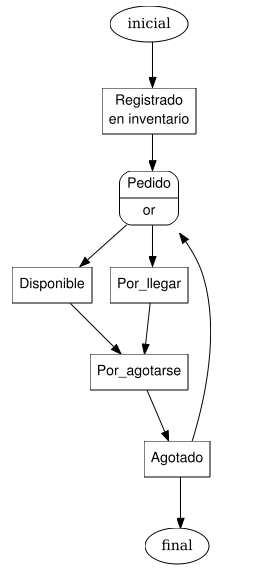
\includegraphics{grafo_inflow7.png}
\caption{\textbf{Figura 34: Agotado}}\label{_templates/Contenido6/Parte4:figura34}\end{figure}
\end{quote}

Descripción de la {\hyperref[_templates/Contenido6/Parte4:figura34]{\emph{Figura 34: Agotado}}}:
\begin{itemize}
\item {} 
La condición del circulo \textbf{inicial} apunta a la primera tarea de cuadro \textbf{Registrado}.

\item {} 
La primera tarea \textbf{Registrado} apunta a la segunda tarea \textbf{Pedido}.

\item {} 
La segunda tarea apunta a 2 tareas, la primera opción de tarea es la del cuadro \textbf{Disponible} y la segunada opción de tarea es la del cuadro \textbf{Por\_llegar}.

\item {} 
Las dos opción de tareas apunta a la quinta tarea del cuadro \textbf{Por\_agotarse}.

\item {} 
La quinta tarea apunta a la sexta tarea del cuadro \textbf{Agotado}.

\item {} 
La sexta tarea apunta a la condición de circulo \textbf{final}.

\item {} 
En esta imagen vemos como se conectan la condición  \textbf{inicial} con la primera tarea \textbf{Registrado}, la tarea primera tarea con la segunda tarea \textbf{Pedido}, la segunda tarea apunta a dos opciones de tareas la cual la primera opción es la tarea \textbf{Disponible} y la segunda opción de tarea \textbf{Por\_llegar}, las dos opciones de tarea apuntan a la quinta tarea \textbf{Por\_agotarse}, la quinta tarea apunta a la sexta tarea \textbf{Agotado} y la sexta tarea apunta a la condición \textbf{final}.

\end{itemize}
\end{notice}

\begin{notice}{note}{Nota:}
Si por algún motivo les causo errores en los pasos aquí están el archivo para que los \textbf{descarguen} como se muestra en la siguiente imagen.
\end{notice}

\textbf{DOWNLOAD:}


\includegraphics{download1.png}

\code{PRODUCTOS.XML}
\end{quote}
\end{quote}


\chapter{\index{Ver datos usando flujos de trabajo}Ver datos usando flujos de trabajo}
\label{_templates/Contenido6/Parte3:ver-datos-usando-flujos-de-trabajo}\label{_templates/Contenido6/Parte3::doc}
En esta sección de explicar las acciones necesarias para obtener reportes asociados a la configuración de datos del directorio \textbf{.safet/ (PySafet)}. Tomando como ejemplo el caso inventario explicaremos las acciones a realizar para obtener un listado de todos los datos.

\textbf{A continuaciones mostraremos las siguientes acciones:}


\section{1° PRIMERA ACCION (Tarea ``vRegistrado'')}
\label{_templates/Contenido6/Parte3:primera-accion-tarea-vregistrado}
Listaremos los productos que se encuentran registrados \textbf{(en estado registrado)}, con la tarea \textbf{vRegistrado} la cual conocimos en los pasos anteriores:


\strong{Ver también:}


\begin{Verbatim}[commandchars=\\\{\}]
\PYG{c}{\PYGZlt{}!\PYGZhy{}\PYGZhy{}}
\PYG{c}{**************}
\PYG{c}{\textbar{} Registrado \textbar{}}
\PYG{c}{**************}
\PYG{c}{\PYGZhy{}\PYGZhy{}\PYGZgt{}}
\PYG{n+nt}{\PYGZlt{}task} \PYG{n+na}{title=}\PYG{l+s}{\PYGZdq{}en inventario\PYGZdq{}} \PYG{n+na}{id=}\PYG{l+s}{\PYGZdq{}Registrado\PYGZdq{}}\PYG{n+nt}{\PYGZgt{}}
\PYG{n+nt}{\PYGZlt{}port} \PYG{n+na}{side=}\PYG{l+s}{\PYGZdq{}forward\PYGZdq{}} \PYG{n+na}{type=}\PYG{l+s}{\PYGZdq{}split\PYGZdq{}}\PYG{n+nt}{\PYGZgt{}}
\PYG{n+nt}{\PYGZlt{}connection} \PYG{n+na}{query=}\PYG{l+s}{\PYGZdq{}true\PYGZdq{}} \PYG{n+na}{options=}\PYG{l+s}{\PYGZdq{}\PYGZdq{}} \PYG{n+na}{source=}\PYG{l+s}{\PYGZdq{}final\PYGZdq{}}\PYG{n+nt}{/\PYGZgt{}}
\PYG{n+nt}{\PYGZlt{}/port\PYGZgt{}}
             \PYG{c}{\PYGZlt{}!\PYGZhy{}\PYGZhy{}}\PYG{c}{ nombre de las columnas(id,nombre,status),  variable(id=\PYGZdq{}vRegistrado\PYGZdq{})}\PYG{c}{\PYGZhy{}\PYGZhy{}\PYGZgt{}}
\PYG{n+nt}{\PYGZlt{}variable} \PYG{n+na}{config=}\PYG{l+s}{\PYGZdq{}1\PYGZdq{}} \PYG{n+na}{documentsource=}\PYG{l+s}{\PYGZdq{}select id,nombre,status from productos\PYGZdq{}}
\PYG{n+na}{type=}\PYG{l+s}{\PYGZdq{}sql\PYGZdq{}} \PYG{n+na}{tokenlink=}\PYG{l+s}{\PYGZdq{}\PYGZdq{}} \PYG{n+na}{id=}\PYG{l+s}{\PYGZdq{}vRegistrado\PYGZdq{}} \PYG{n+na}{rolfield=}\PYG{l+s}{\PYGZdq{}(select rol from productos\PYGZus{}registro}
\PYG{l+s}{where productoid=productos.id and regstatus=\PYGZsq{}Registrado\PYGZsq{}) as rol\PYGZdq{}} \PYG{n+na}{scope=}\PYG{l+s}{\PYGZdq{}task\PYGZdq{}}
\PYG{n+na}{timestampfield=}\PYG{l+s}{\PYGZdq{}(select fecha from productos\PYGZus{}registro}
\PYG{l+s}{where productoid=productos.id and regstatus=\PYGZsq{}Registrado\PYGZsq{}) as fecha\PYGZdq{}}\PYG{n+nt}{/\PYGZgt{}}
\PYG{n+nt}{\PYGZlt{}/task\PYGZgt{}}
\end{Verbatim}




\subsection{1° PRIMER PASO}
\label{_templates/Contenido6/Parte3:primer-paso}\begin{itemize}
\item {} 
Crearemos un directorio en nuestro \textbf{\textless{}HOME\textgreater{}/JsonInterfaz}

\end{itemize}
\begin{quote}

\begin{Verbatim}[commandchars=\\\{\}]
\PYG{n+nv}{\PYGZdl{} }mkdir \PYG{n+nv}{\PYGZdl{}HOME}/JsonInterfaz
\end{Verbatim}
\end{quote}
\begin{itemize}
\item {} 
Crearemos un directorio  que creamos \textbf{JsonInterfaz/}

\end{itemize}
\begin{quote}

\begin{Verbatim}[commandchars=\\\{\}]
\PYG{n+nv}{\PYGZdl{} }\PYG{n+nb}{cd} \PYG{n+nv}{\PYGZdl{}HOME}/JsonInterfaz
\end{Verbatim}
\end{quote}


\subsection{2°  SEGUNDO PASO}
\label{_templates/Contenido6/Parte3:segundo-paso}\begin{itemize}
\item {} 
Crearemos un archivo \textbf{.py} por ejemplo \textbf{ListarProducto.py} en el directorio \textbf{JsonInterfaz/}:

\begin{Verbatim}[commandchars=\\\{\}]
JsonInterfaz\PYG{n+nv}{\PYGZdl{} }touch ListarProducto.py
\end{Verbatim}

\item {} 
Abrimos el archivo \textbf{ListarProducto.py}, insertamos el siguiente código:

\end{itemize}
\begin{quote}

\begin{Verbatim}[commandchars=\\\{\}]
\PYG{c}{\PYGZsh{} \PYGZhy{}*\PYGZhy{} coding: utf\PYGZhy{}8 \PYGZhy{}*\PYGZhy{}}

\PYG{k+kn}{import} \PYG{n+nn}{Safet}
\PYG{k+kn}{import} \PYG{n+nn}{os}

\PYG{n}{myhome} \PYG{o}{=} \PYG{n}{os}\PYG{o}{.}\PYG{n}{getenv}\PYG{p}{(}\PYG{l+s}{\PYGZdq{}}\PYG{l+s}{HOME}\PYG{l+s}{\PYGZdq{}}\PYG{p}{)}
\PYG{n}{mymedia} \PYG{o}{=} \PYG{n}{myhome} \PYG{o}{+} \PYG{l+s}{\PYGZdq{}}\PYG{l+s}{/tmp}\PYG{l+s}{\PYGZdq{}}
\PYG{n}{myurl} \PYG{o}{=} \PYG{l+s}{\PYGZdq{}}\PYG{l+s}{http://localhost}\PYG{l+s}{\PYGZdq{}}

\PYG{n}{myinflow} \PYG{o}{=} \PYG{n}{Safet}\PYG{o}{.}\PYG{n}{MainWindow}\PYG{p}{(}\PYG{n}{myhome}\PYG{p}{)}

\PYG{n}{myinflow}\PYG{o}{.}\PYG{n}{setMediaPath}\PYG{p}{(}\PYG{n}{mymedia} \PYG{p}{)}
\PYG{n}{myinflow}\PYG{o}{.}\PYG{n}{setHostURL}\PYG{p}{(}\PYG{n}{myurl}\PYG{p}{)}


\PYG{n}{myconsult} \PYG{o}{=} \PYG{l+s}{u\PYGZdq{}}\PYG{l+s}{operacion:Listar\PYGZus{}datos\PYGZus{}general }\PYG{l+s+se}{\PYGZbs{}}
\PYG{l+s}{Cargar\PYGZus{}archivo\PYGZus{}flujo: /home/cenditel/.safet/flowfiles/productos.xml }\PYG{l+s+se}{\PYGZbs{}}
\PYG{l+s}{Variable: vRegistrado}\PYG{l+s}{\PYGZdq{}}


\PYG{n}{result} \PYG{o}{=} \PYG{n}{myinflow}\PYG{o}{.}\PYG{n}{login}\PYG{p}{(}\PYG{l+s}{\PYGZdq{}}\PYG{l+s}{admin}\PYG{l+s}{\PYGZdq{}}\PYG{p}{,}\PYG{l+s}{\PYGZdq{}}\PYG{l+s}{admin}\PYG{l+s}{\PYGZdq{}}\PYG{p}{)}

\PYG{k}{if} \PYG{o+ow}{not} \PYG{n}{result}\PYG{p}{:}
    \PYG{k}{print} \PYG{l+s}{\PYGZdq{}}\PYG{l+s}{Authentication failed}\PYG{l+s}{\PYGZdq{}}
    \PYG{n+nb}{exit}\PYG{p}{(}\PYG{p}{)}

\PYG{n}{result} \PYG{o}{=} \PYG{n}{myinflow}\PYG{o}{.}\PYG{n}{toInputConsole}\PYG{p}{(}\PYG{n}{myconsult}\PYG{p}{)}

\PYG{k}{if} \PYG{o+ow}{not} \PYG{n}{result}\PYG{p}{:}
    \PYG{k}{print} \PYG{l+s}{\PYGZdq{}}\PYG{l+s}{Consult failed error: }\PYG{l+s+si}{\PYGZpc{}s}\PYG{l+s}{\PYGZdq{}}  \PYG{o}{\PYGZpc{}} \PYG{p}{(}\PYG{n}{myinflow}\PYG{o}{.}\PYG{n}{currentError}\PYG{p}{(}\PYG{p}{)}\PYG{p}{)}
    \PYG{n+nb}{exit}\PYG{p}{(}\PYG{p}{)}

\PYG{k}{print} \PYG{l+s}{u\PYGZdq{}}\PYG{l+s+si}{\PYGZpc{}s}\PYG{l+s}{\PYGZdq{}} \PYG{o}{\PYGZpc{}} \PYG{p}{(}\PYG{n}{myinflow}\PYG{o}{.}\PYG{n}{currentJSON}\PYG{p}{(}\PYG{p}{)}\PYG{p}{)}
\end{Verbatim}

\begin{notice}{note}{Nota:}
La operación seleccionada es \textbf{``Listar\_datos''}, el archivo donde se realiza la operación es \textbf{``productos.xml''} y el directorio donde se encuentra es \textbf{\textless{}HOMR\textgreater{}.safet/flowfiles/}.
\end{notice}

La variable seleccionada \textbf{``vRegistrado''} se define los siguiente:
\begin{itemize}
\item {} 
La variable debe estar definida en el archivo \textbf{``productos.xml''}.

\item {} 
La operación \textbf{Listar\_datos} esta definida en el archivo \textbf{defconsole.xml} que se encuentra en el directorio \textbf{\textless{}HOME\textgreater{}.safet/input/}

\end{itemize}
\end{quote}


\subsection{3° TERCER PASO}
\label{_templates/Contenido6/Parte3:tercer-paso}\begin{itemize}
\item {} 
Ejecutamos el archivo \textbf{ListarProducto.py} desde la consola de comando como usuario normal:

\end{itemize}
\begin{quote}

\begin{Verbatim}[commandchars=\\\{\}]
JsonInterfaz\PYG{n+nv}{\PYGZdl{} }python ListarProducto.py
\end{Verbatim}

\begin{notice}{note}{Nota:}
Al llamar el método \textbf{toInputConsole} con las opciones dicha anteriormente se generaría el siguiente mensaje \textbf{Json}.

\begin{Verbatim}[commandchars=\\\{\}]
QFSFileEngine::open: No file name specified

 \PYG{c}{\PYGZsh{} Aquí nos indica que se esta conectando a la base de datos}
 \PYG{c}{\PYGZsh{} que esta en el directorio \PYGZlt{}HOME\PYGZgt{}.sefet/}
QSqlDatabasePrivate::removeDatabase:
connection \PYG{l+s+s1}{\PYGZsq{}/home/cenditel/.safet/mydb.db\PYGZsq{}} is still in use,
                              all queries will cease to work.
QSqlDatabasePrivate::removeDatabase:
 connection \PYG{l+s+s1}{\PYGZsq{}/home/cenditel/.safet/mydb.db\PYGZsq{}} is still in use,
                              all queries will cease to work.
QSqlDatabasePrivate::removeDatabase:
 connection \PYG{l+s+s1}{\PYGZsq{}/home/cenditel/.safet/mydb.db\PYGZsq{}} is still in use,
                               all queries will cease to work.

   \PYG{c}{\PYGZsh{} La variable que esta utilizando}
\PYG{o}{\PYGZob{}} \PYG{l+s+s2}{\PYGZdq{}safetvariable\PYGZdq{}} : \PYG{l+s+s2}{\PYGZdq{}vRegistrado\PYGZdq{}},

 \PYG{l+s+s2}{\PYGZdq{}safetkey\PYGZdq{}} : \PYG{l+s+s2}{\PYGZdq{}\PYGZdq{}},

 \PYG{l+s+s2}{\PYGZdq{}safettitle\PYGZdq{}} : \PYG{l+s+s2}{\PYGZdq{}vRegistrado\PYGZdq{}},
 \PYG{l+s+s2}{\PYGZdq{}safetreport\PYGZdq{}} : \PYG{l+s+s2}{\PYGZdq{}operacion:Listar\PYGZus{}datos\PYGZus{}general \PYGZbs{}}
\PYG{l+s+s2}{  Cargar\PYGZus{}archivo\PYGZus{}flujo:/home/cenditel/.safet/flowfiles/productos.xml \PYGZbs{}}
\PYG{l+s+s2}{  Variable: vRegistrado\PYGZdq{}},

  \PYG{c}{\PYGZsh{} Aquí nos dice que hay dos registro en la db}
\PYG{l+s+s2}{\PYGZdq{}safetlistcount\PYGZdq{}} : \PYG{l+s+s2}{\PYGZdq{}2\PYGZdq{}},

 \PYG{c}{\PYGZsh{} Nos mostrara los datos en una lista}
\PYG{l+s+s2}{\PYGZdq{}safetlist\PYGZdq{}} :
\PYG{o}{[}
 \PYG{c}{\PYGZsh{} Aqui nos aparece el nombre de las columnas(id,nombre,status) y}
 \PYG{c}{\PYGZsh{} sus datos}
\PYG{o}{\PYGZob{}}\PYG{l+s+s2}{\PYGZdq{}id\PYGZdq{}}:\PYG{l+s+s2}{\PYGZdq{}1\PYGZdq{}}, \PYG{l+s+s2}{\PYGZdq{}id\PYGZdq{}}:\PYG{l+s+s2}{\PYGZdq{}1\PYGZdq{}}, \PYG{l+s+s2}{\PYGZdq{}nombre\PYGZdq{}}:\PYG{l+s+s2}{\PYGZdq{}Jabón Protex\PYGZdq{}},  \PYG{l+s+s2}{\PYGZdq{}status\PYGZdq{}}:\PYG{l+s+s2}{\PYGZdq{}Registrado\PYGZdq{}}\PYG{o}{\PYGZcb{}},
\PYG{o}{\PYGZob{}}\PYG{l+s+s2}{\PYGZdq{}id\PYGZdq{}}:\PYG{l+s+s2}{\PYGZdq{}2\PYGZdq{}}, \PYG{l+s+s2}{\PYGZdq{}id\PYGZdq{}}:\PYG{l+s+s2}{\PYGZdq{}2\PYGZdq{}}, \PYG{l+s+s2}{\PYGZdq{}nombre\PYGZdq{}}:\PYG{l+s+s2}{\PYGZdq{}Pañales Pamper\PYGZdq{}},\PYG{l+s+s2}{\PYGZdq{}status\PYGZdq{}}:\PYG{l+s+s2}{\PYGZdq{}Registrado\PYGZdq{}}\PYG{o}{\PYGZcb{}}
\PYG{o}{]},

\PYG{c}{\PYGZsh{}Nos mostrara la columnas es decir el keys}
\PYG{l+s+s2}{\PYGZdq{}safetcolumns\PYGZdq{}}  :
\PYG{o}{[}

      \PYG{o}{\PYGZob{}} \PYG{l+s+s2}{\PYGZdq{}key\PYGZdq{}}: \PYG{l+s+s2}{\PYGZdq{}id\PYGZdq{}},\PYG{l+s+s2}{\PYGZdq{}label\PYGZdq{}}:\PYG{l+s+s2}{\PYGZdq{}id\PYGZdq{}},\PYG{l+s+s2}{\PYGZdq{}width\PYGZdq{}}:\PYG{l+s+s2}{\PYGZdq{}10\PYGZdq{}},
      \PYG{l+s+s2}{\PYGZdq{}resizeable\PYGZdq{}}:\PYG{l+s+s2}{\PYGZdq{}true\PYGZdq{}},\PYG{l+s+s2}{\PYGZdq{}sortable\PYGZdq{}}:\PYG{l+s+s2}{\PYGZdq{}true\PYGZdq{}}\PYG{o}{\PYGZcb{}},

      \PYG{o}{\PYGZob{}} \PYG{l+s+s2}{\PYGZdq{}key\PYGZdq{}}: \PYG{l+s+s2}{\PYGZdq{}id\PYGZdq{}},\PYG{l+s+s2}{\PYGZdq{}label\PYGZdq{}}:\PYG{l+s+s2}{\PYGZdq{}id\PYGZdq{}},\PYG{l+s+s2}{\PYGZdq{}width\PYGZdq{}}:\PYG{l+s+s2}{\PYGZdq{}10\PYGZdq{}},
      \PYG{l+s+s2}{\PYGZdq{}resizeable\PYGZdq{}}:\PYG{l+s+s2}{\PYGZdq{}true\PYGZdq{}},\PYG{l+s+s2}{\PYGZdq{}sortable\PYGZdq{}}:\PYG{l+s+s2}{\PYGZdq{}true\PYGZdq{}}\PYG{o}{\PYGZcb{}},

      \PYG{o}{\PYGZob{}} \PYG{l+s+s2}{\PYGZdq{}key\PYGZdq{}}: \PYG{l+s+s2}{\PYGZdq{}nombre\PYGZdq{}},\PYG{l+s+s2}{\PYGZdq{}label\PYGZdq{}}:\PYG{l+s+s2}{\PYGZdq{}nombre\PYGZdq{}},\PYG{l+s+s2}{\PYGZdq{}width\PYGZdq{}}:\PYG{l+s+s2}{\PYGZdq{}90\PYGZdq{}},
      \PYG{l+s+s2}{\PYGZdq{}resizeable\PYGZdq{}}:\PYG{l+s+s2}{\PYGZdq{}true\PYGZdq{}},\PYG{l+s+s2}{\PYGZdq{}sortable\PYGZdq{}}:\PYG{l+s+s2}{\PYGZdq{}true\PYGZdq{}}\PYG{o}{\PYGZcb{}},

      \PYG{o}{\PYGZob{}} \PYG{l+s+s2}{\PYGZdq{}key\PYGZdq{}}: \PYG{l+s+s2}{\PYGZdq{}status\PYGZdq{}},\PYG{l+s+s2}{\PYGZdq{}label\PYGZdq{}}:\PYG{l+s+s2}{\PYGZdq{}status\PYGZdq{}},\PYG{l+s+s2}{\PYGZdq{}width\PYGZdq{}}:\PYG{l+s+s2}{\PYGZdq{}90\PYGZdq{}},
      \PYG{l+s+s2}{\PYGZdq{}resizeable\PYGZdq{}}:\PYG{l+s+s2}{\PYGZdq{}true\PYGZdq{}},\PYG{l+s+s2}{\PYGZdq{}sortable\PYGZdq{}}:\PYG{l+s+s2}{\PYGZdq{}true\PYGZdq{}}\PYG{o}{\PYGZcb{}}
\PYG{o}{]}
\PYG{o}{\PYGZcb{}}
\end{Verbatim}
\end{notice}
\end{quote}


\section{Combinación de Json con HTML(javascript)}
\label{_templates/Contenido6/Parte3:combinacion-de-json-con-html-javascript}
Listaremos los datos con interfaz gráfica de nuestro \textbf{Json}, con los siguientes pasos:


\subsection{1° PRIMER PASO}
\label{_templates/Contenido6/Parte3:id1}\begin{itemize}
\item {} 
Crearemos un archivo \textbf{.py} por ejemplo \textbf{(ScriptJson.py)}, en el directorio \textbf{JsonInterfaz/}:

\end{itemize}
\begin{quote}

\begin{Verbatim}[commandchars=\\\{\}]
JsonInterfaz\PYG{n+nv}{\PYGZdl{} }touch ScriptJson.py
\end{Verbatim}
\phantomsection\label{_templates/Contenido6/Parte3:segundopaso}\end{quote}


\subsection{2° SEGUNDO PASO}
\label{_templates/Contenido6/Parte3:id2}\label{_templates/Contenido6/Parte3:segundopaso}\begin{itemize}
\item {} 
Abrimos el archivo que creamos \textbf{.py(ScriptJson.py)} insertamos el siguiente código:

\end{itemize}
\begin{quote}

\begin{Verbatim}[commandchars=\\\{\}]
\PYG{c}{\PYGZsh{}!/user/bin python}
\PYG{c}{\PYGZsh{} \PYGZhy{}*\PYGZhy{} coding: utf\PYGZhy{}8 \PYGZhy{}*\PYGZhy{}}

\PYG{c}{\PYGZsh{} importamos la librerías a utilizar}
\PYG{k+kn}{import} \PYG{n+nn}{Safet}
\PYG{k+kn}{import} \PYG{n+nn}{os}
\PYG{k+kn}{import} \PYG{n+nn}{json}

\PYG{c}{\PYGZsh{}función para convertir el json en datos con listas}
\PYG{k}{def} \PYG{n+nf}{jsonToJquery}\PYG{p}{(}\PYG{n}{myoldarray}\PYG{p}{)}\PYG{p}{:}

    \PYG{c}{\PYGZsh{} Variables que me van a almacenar listar o arreglos}
    \PYG{n}{mynewarray}  \PYG{o}{=} \PYG{p}{[}\PYG{p}{]}
    \PYG{n}{currcolumns} \PYG{o}{=} \PYG{p}{[}\PYG{p}{]}
    \PYG{n}{currkeys} \PYG{o}{=} \PYG{p}{[}\PYG{p}{]}

    \PYG{c}{\PYGZsh{} Una variable para almacenar}
    \PYG{n}{stringcolumn} \PYG{o}{=} \PYG{l+s}{\PYGZdq{}}\PYG{l+s}{\PYGZdq{}}

    \PYG{c}{\PYGZsh{} Estructura de repetición para obtener}
    \PYG{c}{\PYGZsh{} Las keys es decir los dato de}
    \PYG{c}{\PYGZsh{}      las columnas (id,nombre,status)}
    \PYG{k}{for} \PYG{n}{reg} \PYG{o+ow}{in} \PYG{n}{myoldarray}\PYG{p}{:}
        \PYG{c}{\PYGZsh{} reg.keys() me obtiene una en una la columnas}
        \PYG{n}{currkeys} \PYG{o}{=} \PYG{n}{reg}\PYG{o}{.}\PYG{n}{keys}\PYG{p}{(}\PYG{p}{)}
        \PYG{n}{myvalue} \PYG{o}{=} \PYG{l+s}{\PYGZdq{}}\PYG{l+s}{\PYGZdq{}}
        \PYG{n}{regarray} \PYG{o}{=} \PYG{p}{[}\PYG{p}{]}

        \PYG{c}{\PYGZsh{} Estructura de repetición anidada}
        \PYG{c}{\PYGZsh{} Se obtienen los datos de la columnas}
        \PYG{c}{\PYGZsh{}      es decir del (id,nombre,status)}
        \PYG{k}{for} \PYG{n}{currkey} \PYG{o+ow}{in} \PYG{n}{currkeys}\PYG{p}{:}
            \PYG{c}{\PYGZsh{} optienes el datos}
            \PYG{n}{myvalue}  \PYG{o}{=} \PYG{n}{reg}\PYG{p}{[}\PYG{n}{currkey}\PYG{p}{]}
            \PYG{c}{\PYGZsh{} Insertamos el dato dentro de la lista regarray[]}
            \PYG{n}{regarray}\PYG{o}{.}\PYG{n}{insert}\PYG{p}{(}\PYG{l+m+mi}{0}\PYG{p}{,}\PYG{n}{myvalue}\PYG{p}{)}

        \PYG{c}{\PYGZsh{} Se añade la lista regarray[] es decir datos de las tablas}
        \PYG{n}{mynewarray}\PYG{o}{.}\PYG{n}{append}\PYG{p}{(}\PYG{n}{regarray}\PYG{p}{)}


    \PYG{c}{\PYGZsh{}Estructura de repetición para obtener las columnas para javascript}
    \PYG{k}{for} \PYG{n}{currkey} \PYG{o+ow}{in} \PYG{n}{currkeys}\PYG{p}{:}
        \PYG{c}{\PYGZsh{} Optenemos las columnas que se almacenan en un diccionario}
        \PYG{n}{currcolumn} \PYG{o}{=} \PYG{p}{\PYGZob{}} \PYG{l+s}{\PYGZdq{}}\PYG{l+s}{sTitle}\PYG{l+s}{\PYGZdq{}} \PYG{p}{:} \PYG{n}{currkey} \PYG{p}{\PYGZcb{}}
        \PYG{c}{\PYGZsh{} Se inserta en la lista currcolumn[] el diccionario}
        \PYG{n}{currcolumns}\PYG{o}{.}\PYG{n}{insert}\PYG{p}{(}\PYG{l+m+mi}{0}\PYG{p}{,}\PYG{n}{currcolumn}\PYG{p}{)}

    \PYG{c}{\PYGZsh{} Retornamos la función con 2 listas}
    \PYG{c}{\PYGZsh{} mynewarray[] que son los datos de la tablas o columnas}
    \PYG{c}{\PYGZsh{} currcolumns[] que es un diccionario que contienes las columnas de}
    \PYG{c}{\PYGZsh{}                                          la tablas de los datos}
    \PYG{k}{return} \PYG{p}{(}\PYG{n}{mynewarray}\PYG{p}{,}\PYG{n}{currcolumns}\PYG{p}{)}


\PYG{c}{\PYGZsh{} función para escribir los datos obtenido en un archivo .js(javascript)}
\PYG{k}{def} \PYG{n+nf}{writeJsonData}\PYG{p}{(}\PYG{n}{data}\PYG{p}{,}\PYG{n}{columns}\PYG{p}{,}\PYG{n}{Variable}\PYG{p}{,}\PYG{n}{filename}\PYG{p}{)}\PYG{p}{:}

    \PYG{c}{\PYGZsh{} u\PYGZdq{}\PYGZpc{}s\PYGZdq{} para almacenan los datos y las columnas}
    \PYG{n}{stringnewarray} \PYG{o}{=} \PYG{l+s}{u\PYGZdq{}}\PYG{l+s+si}{\PYGZpc{}s}\PYG{l+s}{\PYGZdq{}} \PYG{o}{\PYGZpc{}}  \PYG{n}{data}
    \PYG{n}{stringcolumns} \PYG{o}{=} \PYG{l+s}{u\PYGZdq{}}\PYG{l+s+si}{\PYGZpc{}s}\PYG{l+s}{\PYGZdq{}} \PYG{o}{\PYGZpc{}} \PYG{n}{columns}

    \PYG{c}{\PYGZsh{} se abre el archivo de tipo escritura}
    \PYG{n+nb}{file} \PYG{o}{=} \PYG{n+nb}{open}\PYG{p}{(}\PYG{n}{filename}\PYG{p}{,} \PYG{l+s}{\PYGZdq{}}\PYG{l+s}{w}\PYG{l+s}{\PYGZdq{}}\PYG{p}{)}

    \PYG{c}{\PYGZsh{} Escribimos el nombre de lista para datos y para las columnas}
    \PYG{n}{datatowrite} \PYG{o}{=} \PYG{l+s}{u\PYGZdq{}}\PYG{l+s}{dataInventory }\PYG{l+s+se}{\PYGZbs{}}
\PYG{l+s}{       = }\PYG{l+s+si}{\PYGZpc{}s}\PYG{l+s+se}{\PYGZbs{}n}\PYG{l+s+se}{\PYGZbs{}n}\PYG{l+s}{columnInventory = }\PYG{l+s+si}{\PYGZpc{}s}\PYG{l+s}{\PYGZdq{}} \PYG{o}{\PYGZpc{}} \PYG{p}{(} \PYG{n}{stringnewarray}\PYG{p}{,} \PYG{n}{stringcolumns} \PYG{p}{)}

    \PYG{c}{\PYGZsh{} Se obtiene el valor de la variable}
    \PYG{n}{variablewrite} \PYG{o}{=} \PYG{l+s}{\PYGZdq{}}\PYG{l+s}{Variable = }\PYG{l+s+si}{\PYGZpc{}s}\PYG{l+s}{\PYGZdq{}} \PYG{o}{\PYGZpc{}} \PYG{p}{(}\PYG{n}{Variable}\PYG{p}{)}

    \PYG{c}{\PYGZsh{} datatowrite.replace para que en el archivo}
    \PYG{c}{\PYGZsh{}                  .js se me eliminar \PYGZdq{}u\PYGZsq{}\PYGZdq{}por \PYGZdq{}\PYGZsq{}\PYGZdq{}}
    \PYG{n}{datatowrite} \PYG{o}{=}  \PYG{n}{datatowrite}\PYG{o}{.}\PYG{n}{replace}\PYG{p}{(}\PYG{l+s}{\PYGZdq{}}\PYG{l+s}{u}\PYG{l+s}{\PYGZsq{}}\PYG{l+s}{\PYGZdq{}}\PYG{p}{,}\PYG{l+s}{\PYGZdq{}}\PYG{l+s}{\PYGZsq{}}\PYG{l+s}{\PYGZdq{}}\PYG{p}{)}
    \PYG{n}{variablewrite} \PYG{o}{=}  \PYG{n}{variablewrite}\PYG{o}{.}\PYG{n}{replace}\PYG{p}{(}\PYG{l+s}{\PYGZdq{}}\PYG{l+s}{u}\PYG{l+s}{\PYGZsq{}}\PYG{l+s}{\PYGZdq{}}\PYG{p}{,}\PYG{l+s}{\PYGZdq{}}\PYG{l+s}{\PYGZsq{}}\PYG{l+s}{\PYGZdq{}}\PYG{p}{)}

    \PYG{c}{\PYGZsh{} salto de linea}
    \PYG{n}{datatowrite} \PYG{o}{=} \PYG{n}{datatowrite} \PYG{o}{+} \PYG{l+s}{\PYGZdq{}}\PYG{l+s+se}{\PYGZbs{}n}\PYG{l+s}{\PYGZdq{}}

    \PYG{c}{\PYGZsh{} Escribimos en archivo las dos listas}
    \PYG{n+nb}{file}\PYG{o}{.}\PYG{n}{write}\PYG{p}{(}\PYG{n}{datatowrite}\PYG{p}{)}
    \PYG{n+nb}{file}\PYG{o}{.}\PYG{n}{write}\PYG{p}{(}\PYG{n}{variablewrite}\PYG{p}{)}

    \PYG{c}{\PYGZsh{} Cerramos el archivo}
    \PYG{n+nb}{file}\PYG{o}{.}\PYG{n}{close}\PYG{p}{(}\PYG{p}{)}

\PYG{c}{\PYGZsh{} Mi función principal}
\PYG{k}{def} \PYG{n+nf}{Principal}\PYG{p}{(}\PYG{p}{)}\PYG{p}{:}

    \PYG{c}{\PYGZsh{} Se localiza en el directorio \PYGZlt{}HOME\PYGZgt{}}
    \PYG{n}{myhome} \PYG{o}{=} \PYG{n}{os}\PYG{o}{.}\PYG{n}{getenv}\PYG{p}{(}\PYG{l+s}{\PYGZdq{}}\PYG{l+s}{HOME}\PYG{l+s}{\PYGZdq{}}\PYG{p}{)}
    \PYG{n}{mymedia} \PYG{o}{=} \PYG{n}{myhome} \PYG{o}{+} \PYG{l+s}{\PYGZdq{}}\PYG{l+s}{/tmp}\PYG{l+s}{\PYGZdq{}}
    \PYG{n}{myurl} \PYG{o}{=} \PYG{l+s}{\PYGZdq{}}\PYG{l+s}{http://localhost}\PYG{l+s}{\PYGZdq{}}

    \PYG{c}{\PYGZsh{} Mi constructor MainWindow}
    \PYG{n}{myinflow} \PYG{o}{=} \PYG{n}{Safet}\PYG{o}{.}\PYG{n}{MainWindow}\PYG{p}{(}\PYG{n}{myhome}\PYG{p}{)}

    \PYG{n}{myinflow}\PYG{o}{.}\PYG{n}{setMediaPath}\PYG{p}{(}\PYG{n}{mymedia} \PYG{p}{)}
    \PYG{n}{myinflow}\PYG{o}{.}\PYG{n}{setHostURL}\PYG{p}{(}\PYG{n}{myurl}\PYG{p}{)}

    \PYG{c}{\PYGZsh{} Mi consulta de vRegistrado y su operación listar datos}
    \PYG{c}{\PYGZsh{}que se encuentra en el directorio \PYGZlt{}HOME\PYGZgt{}.safe/flowfiles/}
    \PYG{n}{myconsult} \PYG{o}{=} \PYG{l+s}{u\PYGZdq{}}\PYG{l+s}{operacion:Listar\PYGZus{}datos }\PYG{l+s+se}{\PYGZbs{}}
\PYG{l+s}{       Cargar\PYGZus{}archivo\PYGZus{}flujo: }\PYG{l+s+si}{\PYGZpc{}s}\PYG{l+s}{/.safet/flowfiles/productos.xml }\PYG{l+s+se}{\PYGZbs{}}
\PYG{l+s}{       Variable: vRegistrado }\PYG{l+s}{\PYGZdq{}} \PYG{o}{\PYGZpc{}} \PYG{p}{(}\PYG{n}{myhome}\PYG{p}{)}

    \PYG{c}{\PYGZsh{} Nombre de usuario y si password}
    \PYG{n}{result} \PYG{o}{=} \PYG{n}{myinflow}\PYG{o}{.}\PYG{n}{login}\PYG{p}{(}\PYG{l+s}{\PYGZdq{}}\PYG{l+s}{admin}\PYG{l+s}{\PYGZdq{}}\PYG{p}{,}\PYG{l+s}{\PYGZdq{}}\PYG{l+s}{admin}\PYG{l+s}{\PYGZdq{}}\PYG{p}{)}

    \PYG{k}{if} \PYG{o+ow}{not} \PYG{n}{result}\PYG{p}{:}
        \PYG{k}{print} \PYG{l+s}{\PYGZdq{}}\PYG{l+s}{Authentication failed}\PYG{l+s}{\PYGZdq{}}
        \PYG{n+nb}{exit}\PYG{p}{(}\PYG{p}{)}

    \PYG{c}{\PYGZsh{} Obtiene los el json de archivo toInputConsole.xml}
    \PYG{n}{result} \PYG{o}{=} \PYG{n}{myinflow}\PYG{o}{.}\PYG{n}{toInputConsole}\PYG{p}{(}\PYG{n}{myconsult}\PYG{p}{)}

    \PYG{k}{if} \PYG{o+ow}{not} \PYG{n}{result}\PYG{p}{:}
        \PYG{k}{print} \PYG{l+s}{\PYGZdq{}}\PYG{l+s}{Consult failed error: }\PYG{l+s+si}{\PYGZpc{}s}\PYG{l+s}{\PYGZdq{}}  \PYG{o}{\PYGZpc{}} \PYG{p}{(}\PYG{n}{myinflow}\PYG{o}{.}\PYG{n}{currentError}\PYG{p}{(}\PYG{p}{)}\PYG{p}{)}
        \PYG{n+nb}{exit}\PYG{p}{(}\PYG{p}{)}

    \PYG{c}{\PYGZsh{} Se obtiene mis datos json}
    \PYG{n}{mystringdata} \PYG{o}{=} \PYG{l+s}{u\PYGZdq{}}\PYG{l+s+si}{\PYGZpc{}s}\PYG{l+s}{\PYGZdq{}} \PYG{o}{\PYGZpc{}} \PYG{n}{myinflow}\PYG{o}{.}\PYG{n}{currentJSON}\PYG{p}{(}\PYG{p}{)}\PYG{p}{;}

    \PYG{c}{\PYGZsh{} Me carga los datos json}
    \PYG{n}{mydata} \PYG{o}{=} \PYG{n}{json}\PYG{o}{.}\PYG{n}{loads}\PYG{p}{(}\PYG{n}{mystringdata}\PYG{p}{)}

    \PYG{c}{\PYGZsh{} Llámanos a la función con el nombre jsonToJquery()}
    \PYG{c}{\PYGZsh{} para modificar el json}
    \PYG{c}{\PYGZsh{} Se le pasa 1 parámetro}
        \PYG{c}{\PYGZsh{} primero mydata con el nombre de la lista}

    \PYG{c}{\PYGZsh{} Se almacenan los datos en 2 variable}
    \PYG{c}{\PYGZsh{} La cual la función esta retornando 2 resultados}
        \PYG{c}{\PYGZsh{}               el array y las columnas del json}
    \PYG{p}{(}\PYG{n}{mynewarray}\PYG{p}{,}\PYG{n}{currcolumns}\PYG{p}{)} \PYG{o}{=} \PYG{n}{jsonToJquery}\PYG{p}{(}\PYG{n}{mydata}\PYG{p}{[}\PYG{l+s}{\PYGZdq{}}\PYG{l+s}{safetlist}\PYG{l+s}{\PYGZdq{}}\PYG{p}{]}\PYG{p}{)}

    \PYG{c}{\PYGZsh{}Llámanos a la función que la llámanos writeJsonData()}
    \PYG{c}{\PYGZsh{}            para insertar los datos en un archivo}
    \PYG{c}{\PYGZsh{}Se le pasan 3 parámetro:}
        \PYG{c}{\PYGZsh{}primero mynewarray}
        \PYG{c}{\PYGZsh{}Segundo currcolumns}
        \PYG{c}{\PYGZsh{}Tercero el nombre del archivo .js}
    \PYG{n}{writeJsonData}\PYG{p}{(}\PYG{n}{mynewarray}\PYG{p}{,}\PYG{n}{currcolumns}\PYG{p}{,}\PYG{p}{[}\PYG{n}{mydata}\PYG{p}{[}\PYG{l+s}{\PYGZdq{}}\PYG{l+s}{safetvariable}\PYG{l+s}{\PYGZdq{}}\PYG{p}{]}\PYG{p}{]}\PYG{p}{,}\PYG{l+s}{\PYGZdq{}}\PYG{l+s}{dataInventory.js}\PYG{l+s}{\PYGZdq{}}\PYG{p}{)}

\PYG{k}{if} \PYG{n}{\PYGZus{}\PYGZus{}name\PYGZus{}\PYGZus{}} \PYG{o}{==} \PYG{l+s}{\PYGZdq{}}\PYG{l+s}{\PYGZus{}\PYGZus{}main\PYGZus{}\PYGZus{}}\PYG{l+s}{\PYGZdq{}}\PYG{p}{:}

    \PYG{c}{\PYGZsh{} Mi función principal}
    \PYG{n}{Principal}\PYG{p}{(}\PYG{p}{)}
\end{Verbatim}

\begin{notice}{note}{Nota:}
\textbf{Este Script se utiliza para poder ver los datos con la libreria jquery de manara más dinamica.}
\end{notice}
\phantomsection\label{_templates/Contenido6/Parte3:tercerpaso}\end{quote}


\subsection{3° TERCER PASO}
\label{_templates/Contenido6/Parte3:tercerpaso}\label{_templates/Contenido6/Parte3:id3}\begin{itemize}
\item {} 
Ejecutamos el archivo \textbf{.py(ScriptJson.py)} desde la consola de comando como usuario normal:

\end{itemize}
\begin{quote}

\begin{Verbatim}[commandchars=\\\{\}]
JsonInterfaz\PYG{n+nv}{\PYGZdl{} }python ScriptJson.py
\end{Verbatim}

\begin{notice}{note}{Nota:}
\textbf{Nos mostrara el siguiente mensaje, significando que funciono correctamente el Script}

\begin{Verbatim}[commandchars=\\\{\}]
 QFSFileEngine::open: No file name specified
 QSqlDatabasePrivate::removeDatabase: connection \PYG{l+s+s1}{\PYGZsq{}/home/cenditel/}
\PYG{l+s+s1}{.safet/mydb.db\PYGZsq{}} is still in use, all queries will cease to work.
 QSqlDatabasePrivate::removeDatabase: connection \PYG{l+s+s1}{\PYGZsq{}/home/cenditel/}
\PYG{l+s+s1}{.safet/mydb.db\PYGZsq{}} is still in use, all queries will cease to work.
 QSqlDatabasePrivate::removeDatabase: connection \PYG{l+s+s1}{\PYGZsq{}/home/cenditel/}
\PYG{l+s+s1}{.safet/mydb.db\PYGZsq{}} is still in use, all queries will cease to work.
\end{Verbatim}
\end{notice}

\begin{notice}{note}{Nota:}
AL ejecutar Script \textbf{(ScriptJson.py)} se genera un archivo \textbf{javascript} llamado \textbf{dataInventory.js} que contiene las columnas de la tabla y sus datos
\end{notice}
\end{quote}


\subsection{4° CUARTO PASO}
\label{_templates/Contenido6/Parte3:cuarto-paso}\begin{itemize}
\item {} 
Crearemos un archivo \textbf{.html} por ejemplo \textbf{(InventarioJson.html)}, en el directorio \textbf{JsonInterfaz/}:

\end{itemize}
\begin{quote}

\begin{Verbatim}[commandchars=\\\{\}]
JsonInterfaz\PYG{n+nv}{\PYGZdl{} }touch InventarioJson.html
\end{Verbatim}
\end{quote}
\begin{itemize}
\item {} 
Abrimos el archivo que creamos \textbf{.html(InventarioJson.html)}, insertamos el siguiente código:

\end{itemize}
\begin{quote}

\begin{Verbatim}[commandchars=\\\{\}]
\PYG{n+nt}{\PYGZlt{}html}\PYG{n+nt}{\PYGZgt{}}
\PYG{n+nt}{\PYGZlt{}head}\PYG{n+nt}{\PYGZgt{}}


  \PYG{n+nt}{\PYGZlt{}link} \PYG{n+na}{rel=}\PYG{l+s}{\PYGZdq{}stylesheet\PYGZdq{}} \PYG{n+na}{type=}\PYG{l+s}{\PYGZdq{}text/css\PYGZdq{}}
  \PYG{n+na}{href=}\PYG{l+s}{\PYGZdq{}http://ajax.aspnetcdn.com/ajax/}
\PYG{l+s}{      jquery.dataTables/1.9.4/css/jquery.dataTables.css\PYGZdq{}}\PYG{n+nt}{\PYGZgt{}}
\PYG{n+nt}{\PYGZlt{}/head\PYGZgt{}}

\PYG{n+nt}{\PYGZlt{}body}\PYG{n+nt}{\PYGZgt{}}

\PYG{c}{\PYGZlt{}!\PYGZhy{}\PYGZhy{}}\PYG{c}{ Aqui se crea la tabla dentro de la etiqueta \PYGZlt{}body\PYGZgt{}}\PYG{c}{\PYGZhy{}\PYGZhy{}\PYGZgt{}}
\PYG{n+nt}{\PYGZlt{}table} \PYG{n+na}{cellpadding=}\PYG{l+s}{\PYGZdq{}0\PYGZdq{}} \PYG{n+na}{cellspacing=}\PYG{l+s}{\PYGZdq{}0\PYGZdq{}} \PYG{n+na}{border=}\PYG{l+s}{\PYGZdq{}0\PYGZdq{}}
      \PYG{n+na}{class=}\PYG{l+s}{\PYGZdq{}display\PYGZdq{}} \PYG{n+na}{name=}\PYG{l+s}{\PYGZdq{}safettable0\PYGZdq{}} \PYG{n+na}{id=}\PYG{l+s}{\PYGZdq{}safettable0\PYGZdq{}}\PYG{n+nt}{\PYGZgt{}}
\PYG{n+nt}{\PYGZlt{}/table\PYGZgt{}}

\PYG{n+nt}{\PYGZlt{}script }\PYG{n+na}{src=}\PYG{l+s}{\PYGZdq{}dataInventory.js\PYGZdq{}}\PYG{n+nt}{\PYGZgt{}} \PYG{n+nt}{\PYGZlt{}/script\PYGZgt{}}

\PYG{n+nt}{\PYGZlt{}script }\PYG{n+na}{type=}\PYG{l+s}{\PYGZdq{}text/javascript\PYGZdq{}} \PYG{n+na}{charset=}\PYG{l+s}{\PYGZdq{}utf8\PYGZdq{}}
 \PYG{n+na}{src=}\PYG{l+s}{\PYGZdq{}http://ajax.aspnetcdn.com/ajax/jQuery/jquery\PYGZhy{}1.8.2.min.js\PYGZdq{}}\PYG{n+nt}{\PYGZgt{}}
\PYG{n+nt}{\PYGZlt{}/script\PYGZgt{}}

\PYG{n+nt}{\PYGZlt{}script }\PYG{n+na}{type=}\PYG{l+s}{\PYGZdq{}text/javascript\PYGZdq{}} \PYG{n+na}{charset=}\PYG{l+s}{\PYGZdq{}utf8\PYGZdq{}}
 \PYG{n+na}{src=}\PYG{l+s}{\PYGZdq{}http://ajax.aspnetcdn.com/ajax/}
\PYG{l+s}{              jquery.dataTables/1.9.4/jquery.dataTables.min.js\PYGZdq{}}\PYG{n+nt}{\PYGZgt{}}
\PYG{n+nt}{\PYGZlt{}/script\PYGZgt{}}

\PYG{n+nt}{\PYGZlt{}script}\PYG{n+nt}{\PYGZgt{}}

  \PYG{n+nx}{\PYGZdl{}}\PYG{p}{(}\PYG{k+kd}{function}\PYG{p}{(}\PYG{p}{)}\PYG{p}{\PYGZob{}}
     \PYG{n+nx}{\PYGZdl{}}\PYG{p}{(}\PYG{l+s+s2}{\PYGZdq{}\PYGZsh{}safettable0\PYGZdq{}}\PYG{p}{)}\PYG{p}{.}\PYG{n+nx}{dataTable}\PYG{p}{(}\PYG{p}{\PYGZob{}}
     \PYG{l+s+s2}{\PYGZdq{}aaData\PYGZdq{}}\PYG{o}{:} \PYG{n+nx}{dataInventory}\PYG{p}{,}
     \PYG{l+s+s2}{\PYGZdq{}aoColumns\PYGZdq{}}\PYG{o}{:} \PYG{n+nx}{columnInventory}
     \PYG{p}{\PYGZcb{}}\PYG{p}{)}\PYG{p}{;}
  \PYG{p}{\PYGZcb{}}\PYG{p}{)}
\PYG{n+nt}{\PYGZlt{}/script\PYGZgt{}}

\PYG{n+nt}{\PYGZlt{}/body\PYGZgt{}}
\PYG{n+nt}{\PYGZlt{}/html\PYGZgt{}}
\end{Verbatim}

\begin{notice}{note}{Nota:}
\textbf{En este código HTML se utilizó la librería (jquery) y la librería (jquery.dataTables) de manera interna. Para ver los datos mas dinámicos utilizando (javascript y  json).}
\end{notice}
\end{quote}


\subsection{5° QUINTO PASO}
\label{_templates/Contenido6/Parte3:quinto-paso}\begin{itemize}
\item {} 
Abrimos con cualquier navegador web el archivo Json.html y no mostrara de la siguiente forma: {\hyperref[_templates/Contenido6/Parte3:figura40]{\emph{Figura 28: Json}}}

\end{itemize}
\begin{quote}

\begin{notice}{note}{Nota:}\begin{quote}
\begin{figure}[htbp]
\centering
\capstart

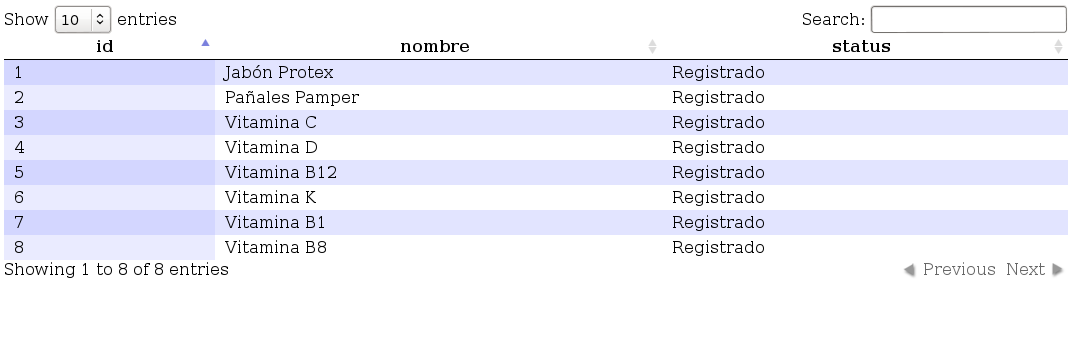
\includegraphics{json.png}
\caption{\textbf{Figura 28: Json}}\label{_templates/Contenido6/Parte3:figura40}\end{figure}
\end{quote}

\textbf{La siguiente} {\hyperref[_templates/Contenido6/Parte3:figura40]{\emph{Figura 28: Json}}} \textbf{indica lo siguiente:}
\begin{itemize}
\item {} 
Nos mostrara el nombre de las columnas.

\item {} 
Nos mostrara los datos de cada columna.

\item {} 
Nos mostrara un buscador \textbf{Search}.

\item {} 
Nos mostrara \textbf{Show} que nos indicara
cuantos datos quiere que se muestren en la tabla.

\end{itemize}
\end{notice}
\end{quote}
\begin{itemize}
\item {} 
Aquí esta el ejemplo, damos \textbf{Clik} a JSON.HTML

\end{itemize}


\subsection{6° SEXTO PASO}
\label{_templates/Contenido6/Parte3:json-html}\label{_templates/Contenido6/Parte3:sexto-paso}
En el script de \textbf{Combinación de Json con HTML(javascript)} del {\hyperref[_templates/Contenido6/Parte3:segundopaso]{\emph{2° SEGUNDO PASO}}} en la función principal tenemos la consulta, la cual nos sirve para consultar los datos de las más variables, es decir, de las variables \textbf{(``vPedido'',''vDisponible'',''vPor\_llegar'',''vPor\_agotarse'',''vAgotado'')}, con solo cambiarle el nombre de la variable.

Por ejemplo habíamos colocado anteriormente la variable \textbf{``vRegistrado''}, la cambiamos por \textbf{``vDisponible''} o la que sea.

Ya cambiado la variable solo se ejecuta el \textbf{Script} como en el {\hyperref[_templates/Contenido6/Parte4:tercerpaso]{\emph{Etiquetas Principales}}}, la cual al ejecutarlo nos generara el archivo \textbf{.js(ScriptJson.py)} con los datos y las columnas, como lo hacia con la variable \textbf{``vRegistrado''}, igualmente vemos en el navegador con el mismo código \textbf{HTML} del archivo \textbf{(InventarioJson.html)}, que nos muestra el contenido con el mismo formato de la librerías \textbf{(jquery y jquery.dataTables)}.


\strong{Ver también:}


\begin{notice}{note}{Nota:}
\textbf{Si vamos a utilizar la variable ``vPedido'' tómese en cuenta lo siguiente:}
\end{notice}


\begin{enumerate}
\item {} 
La varible \textbf{``vPedio''} necesita saber la \textbf{cantidad} de pedidos, para poder mostrar los datos.

\item {} 
Abrimos el archivo \textbf{.xml(productos.xml)} de directorio \textbf{\textless{}HOME\textgreater{}.safet/flowfiles/}:
\begin{quote}

\begin{notice}{note}{Nota:}
Vemos el código y tenemos los atributos \textbf{(id,nombre,status)}:

\begin{Verbatim}[commandchars=\\\{\}]
\PYG{c}{\PYGZlt{}!\PYGZhy{}\PYGZhy{}}
\PYG{c}{**********}
\PYG{c}{\textbar{} Pedido \textbar{}}
\PYG{c}{**********}
\PYG{c}{\PYGZhy{}\PYGZhy{}\PYGZgt{}}
\PYG{n+nt}{\PYGZlt{}task} \PYG{n+na}{title=}\PYG{l+s}{\PYGZdq{}\PYGZdq{}} \PYG{n+na}{id=}\PYG{l+s}{\PYGZdq{}Pedido\PYGZdq{}} \PYG{n+na}{textualinfo=}\PYG{l+s}{\PYGZdq{}\PYGZdq{}}\PYG{n+nt}{\PYGZgt{}}
\PYG{n+nt}{\PYGZlt{}port} \PYG{n+na}{pattern=}\PYG{l+s}{\PYGZdq{}none\PYGZdq{}} \PYG{n+na}{side=}\PYG{l+s}{\PYGZdq{}forward\PYGZdq{}} \PYG{n+na}{type=}\PYG{l+s}{\PYGZdq{}split\PYGZdq{}}\PYG{n+nt}{\PYGZgt{}}
\PYG{n+nt}{\PYGZlt{}connection} \PYG{n+na}{query=}\PYG{l+s}{\PYGZdq{}true\PYGZdq{}} \PYG{n+na}{options=}\PYG{l+s}{\PYGZdq{}\PYGZdq{}} \PYG{n+na}{source=}\PYG{l+s}{\PYGZdq{}final\PYGZdq{}}\PYG{n+nt}{/\PYGZgt{}}
\PYG{n+nt}{\PYGZlt{}/port\PYGZgt{}}

                      \PYG{c}{\PYGZlt{}!\PYGZhy{}\PYGZhy{}}\PYG{c}{ atributos (id,nombre,status) }\PYG{c}{\PYGZhy{}\PYGZhy{}\PYGZgt{}}
\PYG{n+nt}{\PYGZlt{}variable} \PYG{n+na}{config=}\PYG{l+s}{\PYGZdq{}1\PYGZdq{}} \PYG{n+na}{documentsource=}\PYG{l+s}{\PYGZdq{}select id,nombre,status from productos\PYGZdq{}}
\PYG{n+na}{type=}\PYG{l+s}{\PYGZdq{}sql\PYGZdq{}} \PYG{n+na}{tokenlink=}\PYG{l+s}{\PYGZdq{}\PYGZdq{}}
\PYG{n+na}{id=}\PYG{l+s}{\PYGZdq{}vPedido\PYGZdq{}} \PYG{n+na}{rolfield=}\PYG{l+s}{\PYGZdq{}(select rol from\PYGZam{}\PYGZsh{}xa;productos\PYGZus{}registro}
\PYG{l+s}{where productoid=productos.id and regstatus=\PYGZsq{}Pedido\PYGZsq{}) as rol\PYGZdq{}} \PYG{n+na}{scope=}\PYG{l+s}{\PYGZdq{}task\PYGZdq{}}
\PYG{n+na}{timestampfield=}\PYG{l+s}{\PYGZdq{}(select fecha from productos\PYGZus{}registro}
\PYG{l+s}{where productoid=productos.id and regstatus=\PYGZsq{}Pedido\PYGZsq{}) as fecha\PYGZdq{}}\PYG{n+nt}{/\PYGZgt{}}
\PYG{n+nt}{\PYGZlt{}/task\PYGZgt{}}
\end{Verbatim}
\end{notice}
\end{quote}

\item {} 
Se le decimos que nos muestre el atributo \textbf{cantidad} de la siguiente manera:
\begin{quote}


\strong{Ver también:}


\begin{Verbatim}[commandchars=\\\{\}]
\PYG{c}{\PYGZlt{}!\PYGZhy{}\PYGZhy{}}
\PYG{c}{**********}
\PYG{c}{\textbar{} Pedido \textbar{}}
\PYG{c}{**********}
\PYG{c}{\PYGZhy{}\PYGZhy{}\PYGZgt{}}
\PYG{n+nt}{\PYGZlt{}task} \PYG{n+na}{title=}\PYG{l+s}{\PYGZdq{}\PYGZdq{}} \PYG{n+na}{id=}\PYG{l+s}{\PYGZdq{}Pedido\PYGZdq{}} \PYG{n+na}{textualinfo=}\PYG{l+s}{\PYGZdq{}\PYGZdq{}}\PYG{n+nt}{\PYGZgt{}}
     \PYG{n+nt}{\PYGZlt{}port} \PYG{n+na}{pattern=}\PYG{l+s}{\PYGZdq{}none\PYGZdq{}} \PYG{n+na}{side=}\PYG{l+s}{\PYGZdq{}forward\PYGZdq{}} \PYG{n+na}{type=}\PYG{l+s}{\PYGZdq{}split\PYGZdq{}}\PYG{n+nt}{\PYGZgt{}}
     \PYG{n+nt}{\PYGZlt{}connection} \PYG{n+na}{query=}\PYG{l+s}{\PYGZdq{}true\PYGZdq{}} \PYG{n+na}{options=}\PYG{l+s}{\PYGZdq{}\PYGZdq{}} \PYG{n+na}{source=}\PYG{l+s}{\PYGZdq{}final\PYGZdq{}}\PYG{n+nt}{/\PYGZgt{}}
\PYG{n+nt}{\PYGZlt{}/port\PYGZgt{}}

                                \PYG{c}{\PYGZlt{}!\PYGZhy{}\PYGZhy{}}\PYG{c}{ atributos (id,nombre,cantidad,status) }\PYG{c}{\PYGZhy{}\PYGZhy{}\PYGZgt{}}
     \PYG{n+nt}{\PYGZlt{}variable} \PYG{n+na}{config=}\PYG{l+s}{\PYGZdq{}1\PYGZdq{}} \PYG{n+na}{documentsource=}\PYG{l+s}{\PYGZdq{}select id,nombre,cantidad,status from productos\PYGZdq{}}
     \PYG{n+na}{type=}\PYG{l+s}{\PYGZdq{}sql\PYGZdq{}} \PYG{n+na}{tokenlink=}\PYG{l+s}{\PYGZdq{}\PYGZdq{}}
     \PYG{n+na}{id=}\PYG{l+s}{\PYGZdq{}vPedido\PYGZdq{}} \PYG{n+na}{rolfield=}\PYG{l+s}{\PYGZdq{}(select rol from\PYGZam{}\PYGZsh{}xa;productos\PYGZus{}registro}
\PYG{l+s}{     where productoid=productos.id and regstatus=\PYGZsq{}Pedido\PYGZsq{}) as rol\PYGZdq{}} \PYG{n+na}{scope=}\PYG{l+s}{\PYGZdq{}task\PYGZdq{}}
     \PYG{n+na}{timestampfield=}\PYG{l+s}{\PYGZdq{}(select fecha from productos\PYGZus{}registro}
\PYG{l+s}{     where productoid=productos.id and regstatus=\PYGZsq{}Pedido\PYGZsq{}) as fecha\PYGZdq{}}\PYG{n+nt}{/\PYGZgt{}}
\PYG{n+nt}{\PYGZlt{}/task\PYGZgt{}}
\end{Verbatim}


\end{quote}

\item {} 
Listo ya podemos utilizar la variable \textbf{``vPedido''} para consultar, por ejemplo cuantos productos se han pedido. Claro colocanod la varible \textbf{vPedido} y luego ejecutando el Script del {\hyperref[_templates/Contenido6/Parte3:segundopaso]{\emph{2° SEGUNDO PASO}}}, como en la {\hyperref[_templates/Contenido6/Parte3:figura43]{\emph{Figura 29: Json}}}

\end{enumerate}
\begin{quote}

\begin{notice}{note}{Nota:}\begin{quote}
\begin{figure}[htbp]
\centering
\capstart

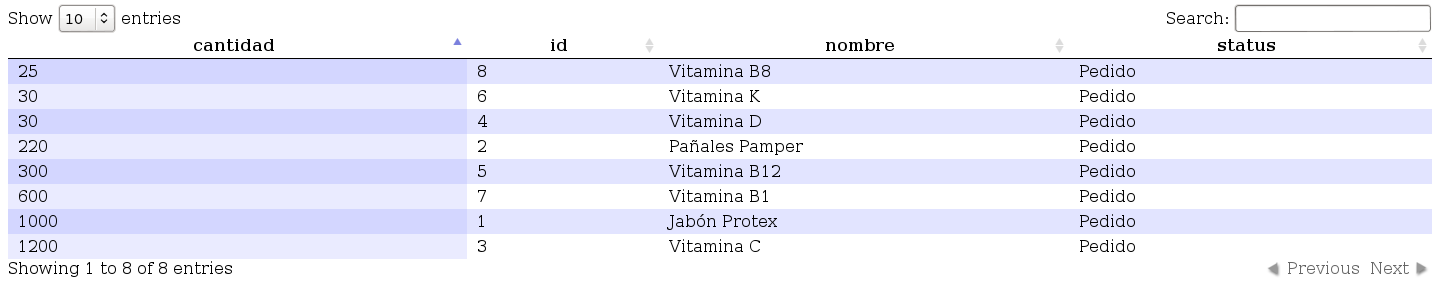
\includegraphics{json1.png}
\caption{\textbf{Figura 29: Json}}\label{_templates/Contenido6/Parte3:figura43}\end{figure}
\end{quote}

\textbf{La siguiente} {\hyperref[_templates/Contenido6/Parte3:figura43]{\emph{Figura 29: Json}}} \textbf{indica lo siguiente:}
\begin{itemize}
\item {} 
Nos mostrara el nombre de las columnas, más el atributo \textbf{cantidad}.

\item {} 
Nos mostrara los datos de cada columna.

\item {} 
Nos mostrara un buscador \textbf{Search}.

\item {} 
Nos mostrara \textbf{Show} que nos indicara
cuantos datos quiere que se muestren en la tabla.

\end{itemize}
\end{notice}
\end{quote}
\begin{itemize}
\item {} 
Aquí esta el ejemplo, damos \textbf{Clik} a JSON.(HTML)

\end{itemize}


\chapter{Ver fichas usando flujos de trabajo}
\label{_templates/Contenido6/Parte5:ver-fichas-usando-flujos-de-trabajo}\label{_templates/Contenido6/Parte5:id4}\label{_templates/Contenido6/Parte5::doc}
En los pasos anteriores obtenemos los datos de dos \textbf{acciones} \textbf{vRegistrado} y \textbf{vPedido}, la cual utilizamos como ejemplo como se muestra en la siguiente imágenes:
\begin{quote}

\begin{notice}{note}{Nota:}
\textbf{vRegistrado}
\begin{quote}
\begin{figure}[htbp]
\centering
\capstart

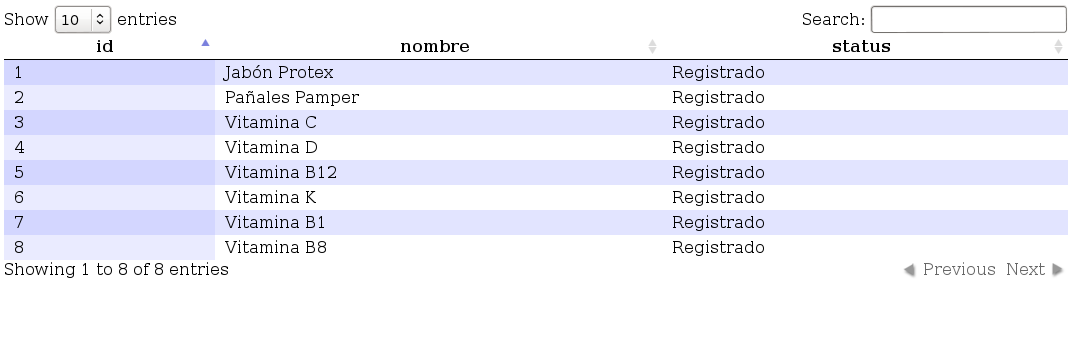
\includegraphics{json.png}
\caption{\textbf{Figura 28: vRegistrado}}\label{_templates/Contenido6/Parte5:figura41}\end{figure}
\end{quote}

\textbf{La siguiente} {\hyperref[_templates/Contenido6/Parte5:figura41]{\emph{Figura 28: vRegistrado}}} \textbf{indica lo siguiente:}
\begin{itemize}
\item {} 
Nos mostrara el nombre de las columnas.

\item {} 
Nos mostrara los datos de cada columna.

\item {} 
Nos mostrara un buscador \textbf{Search}.

\item {} 
Nos mostrara \textbf{Show} que nos indicara
cuantos datos quiere que se muestren en la tabla.

\end{itemize}
\end{notice}

\begin{notice}{note}{Nota:}
\textbf{vPedido}
\begin{quote}
\begin{figure}[htbp]
\centering
\capstart

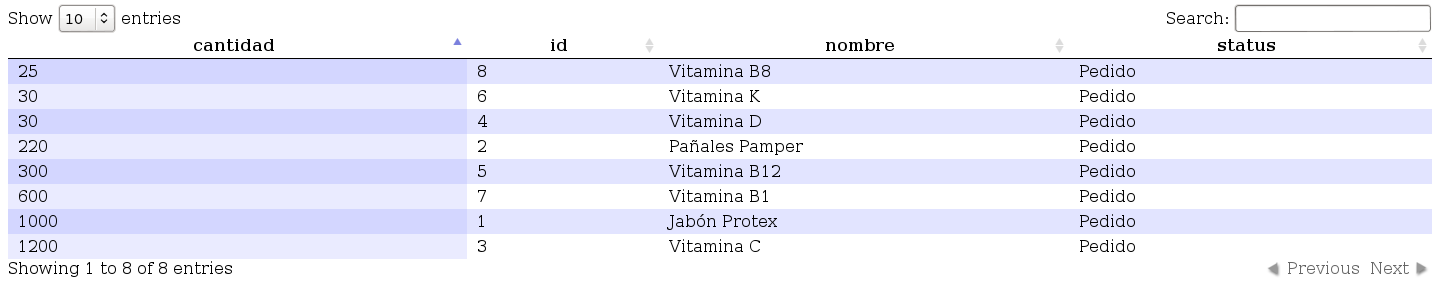
\includegraphics{json1.png}
\caption{\textbf{Figura 29: vPedido}}\label{_templates/Contenido6/Parte5:figura44}\end{figure}
\end{quote}

\textbf{La siguiente} {\hyperref[_templates/Contenido6/Parte5:figura44]{\emph{Figura 29: vPedido}}} \textbf{indica lo siguiente:}
\begin{itemize}
\item {} 
Nos mostrara el nombre de las columnas, más el atributo \textbf{cantidad}.

\item {} 
Nos mostrara los datos de cada columna.

\item {} 
Nos mostrara un buscador \textbf{Search}.

\item {} 
Nos mostrara \textbf{Show} que nos indicara
cuantos datos quiere que se muestren en la tabla.

\end{itemize}
\end{notice}
\end{quote}

\textbf{A continuación vamos a demostrar, como obtener fichas de esa tabla de datos:}


\section{Ficha (vRegistrado) (vPedido)}
\label{_templates/Contenido6/Parte5:ficha-vregistrado-vpedido}
Los paso para obtener una ficha que vamos a seguir mas adelante, nos sirven para las demás acciones menos una, es decir, no solo para la acción \textbf{vRegistrado} sino tambien para las acciones \textbf{(vDisponible,vPor\_llegar,vPor\_agotarse,vAgotado)}. Para la acción \textbf{vPedido} los pason son diferentes ya que ah esta acción se agrega el el atributo \textbf{cantidad}, porque para mostrar los datos depende del valor cantidad.

Las demas acciones tienen, el mismo esquemas de mostrar los datos en fichas como se muestra en la siguiente imagen {\hyperref[_templates/Contenido6/Parte5:figura45]{\emph{Figura 30: Ficha vRegistrado}}}:

\begin{notice}{note}{Nota:}
La imagen nos muestra el nombre de la ficha la cual sirve para las acciones \textbf{(vDisponible,vPor\_llegar,vPor\_agotarse,vAgotado)}, la cual tienen los mismos atributos que las demás acciones.
\begin{quote}
\begin{figure}[htbp]
\centering
\capstart

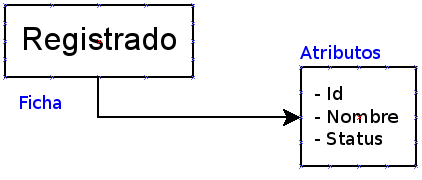
\includegraphics{ficha1.png}
\caption{\textbf{Figura 30: Ficha vRegistrado}}\label{_templates/Contenido6/Parte5:figura45}\end{figure}
\end{quote}

La imagen muestra el nombre de la ficha y sus atributos: {\hyperref[_templates/Contenido6/Parte5:figura50]{\emph{Figura 32: Ficha vPedido}}}
\begin{quote}
\begin{figure}[htbp]
\centering
\capstart

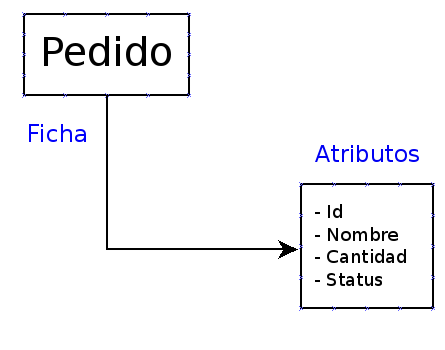
\includegraphics{ficha2.png}
\caption{\textbf{Figura 32: Ficha vPedido}}\label{_templates/Contenido6/Parte5:figura50}\end{figure}
\end{quote}
\end{notice}


\subsection{1° PRIMER PASO}
\label{_templates/Contenido6/Parte5:primer-paso}\begin{itemize}
\item {} 
Nos vamos directorio que hemos creado anteriormente que se llama \textbf{JsonInterfaz/}

\end{itemize}
\begin{quote}

\begin{Verbatim}[commandchars=\\\{\}]
\PYG{n+nv}{\PYGZdl{} }\PYG{n+nb}{cd} \PYG{n+nv}{\PYGZdl{}HOME}/JsonInterfaz
\end{Verbatim}
\end{quote}


\subsection{2° SEGUNDO PASO}
\label{_templates/Contenido6/Parte5:segundo-paso}\begin{itemize}
\item {} 
Ejecutamos el Scritp que insertamos en el archivo que creamos anteriormente \textbf{.py(ScriptJson.py)}, con la varible \textbf{(vRegistrado)} o con la la variable \textbf{vPedido} o la que guste.

\end{itemize}
\begin{quote}

\begin{Verbatim}[commandchars=\\\{\}]
JsonInterfaz\PYGZdl{} python ScriptJson.py
\end{Verbatim}
\end{quote}


\subsection{3° TERCER PASO}
\label{_templates/Contenido6/Parte5:tercer-paso}\begin{itemize}
\item {} 
Crearemos un archivo \textbf{.css} por ejemplo \textbf{(style.css)}, en el directorio \textbf{JsonInterfaz/}:

\end{itemize}
\begin{quote}

\begin{Verbatim}[commandchars=\\\{\}]
JsonInterfaz\PYG{n+nv}{\PYGZdl{} }touch style.css
\end{Verbatim}
\end{quote}
\begin{itemize}
\item {} 
Abrimos el archivo que creamos \textbf{.css(style.css)}, insertamos el siguiente código:

\end{itemize}
\begin{quote}

\begin{Verbatim}[commandchars=\\\{\}]
\PYG{n+nt}{body} \PYG{p}{\PYGZob{}}
        \PYG{k}{background\PYGZhy{}repeat}\PYG{o}{:}\PYG{k}{no\PYGZhy{}repeat}\PYG{p}{;}
        \PYG{k}{background\PYGZhy{}position}\PYG{o}{:}\PYG{k}{top} \PYG{k}{center}\PYG{p}{;}
        \PYG{k}{background\PYGZhy{}color}\PYG{o}{:}\PYG{l+m}{\PYGZsh{}657077}\PYG{p}{;}
        \PYG{k}{margin}\PYG{o}{:}\PYG{l+m}{40px}\PYG{p}{;}
\PYG{p}{\PYGZcb{}}

\PYG{n+nf}{\PYGZsh{}tabbed\PYGZus{}box\PYGZus{}1} \PYG{p}{\PYGZob{}}
        \PYG{k}{margin}\PYG{o}{:} \PYG{l+m}{0px} \PYG{k}{auto} \PYG{l+m}{0px} \PYG{k}{auto}\PYG{p}{;}
        \PYG{k}{width}\PYG{o}{:}\PYG{l+m}{300px}\PYG{p}{;}
\PYG{p}{\PYGZcb{}}
\PYG{n+nc}{.tabbed\PYGZus{}box} \PYG{n+nt}{h4} \PYG{p}{\PYGZob{}}
        \PYG{k}{font\PYGZhy{}family}\PYG{o}{:}\PYG{n}{Arial}\PYG{o}{,} \PYG{n}{Helvetica}\PYG{o}{,} \PYG{k}{sans\PYGZhy{}serif}\PYG{p}{;}
        \PYG{k}{font\PYGZhy{}size}\PYG{o}{:}\PYG{l+m}{23px}\PYG{p}{;}
        \PYG{k}{color}\PYG{o}{:}\PYG{l+m}{\PYGZsh{}ffffff}\PYG{p}{;}
        \PYG{k}{letter\PYGZhy{}spacing}\PYG{o}{:\PYGZhy{}}\PYG{l+m}{1px}\PYG{p}{;}
        \PYG{k}{margin\PYGZhy{}bottom}\PYG{o}{:}\PYG{l+m}{10px}\PYG{p}{;}
\PYG{p}{\PYGZcb{}}
\PYG{n+nc}{.tabbed\PYGZus{}box} \PYG{n+nt}{h4} \PYG{n+nt}{small} \PYG{p}{\PYGZob{}}
        \PYG{k}{color}\PYG{o}{:}\PYG{l+m}{\PYGZsh{}e3e9ec}\PYG{p}{;}
        \PYG{k}{font\PYGZhy{}weight}\PYG{o}{:}\PYG{k}{normal}\PYG{p}{;}
        \PYG{k}{font\PYGZhy{}size}\PYG{o}{:}\PYG{l+m}{9px}\PYG{p}{;}
        \PYG{k}{font\PYGZhy{}family}\PYG{o}{:}\PYG{n}{Verdana}\PYG{o}{,} \PYG{n}{Arial}\PYG{o}{,} \PYG{n}{Helvetica}\PYG{o}{,} \PYG{k}{sans\PYGZhy{}serif}\PYG{p}{;}
        \PYG{k}{text\PYGZhy{}transform}\PYG{o}{:}\PYG{k}{uppercase}\PYG{p}{;}
        \PYG{k}{position}\PYG{o}{:}\PYG{k}{relative}\PYG{p}{;}
        \PYG{k}{top}\PYG{o}{:\PYGZhy{}}\PYG{l+m}{4px}\PYG{p}{;}
        \PYG{k}{left}\PYG{o}{:}\PYG{l+m}{6px}\PYG{p}{;}
        \PYG{k}{letter\PYGZhy{}spacing}\PYG{o}{:}\PYG{l+m}{0px}\PYG{p}{;}
\PYG{p}{\PYGZcb{}}
\PYG{n+nc}{.tabbed\PYGZus{}area} \PYG{p}{\PYGZob{}}
        \PYG{k}{border}\PYG{o}{:}\PYG{l+m}{1px} \PYG{k}{solid} \PYG{l+m}{\PYGZsh{}494e52}\PYG{p}{;}
        \PYG{k}{background\PYGZhy{}color}\PYG{o}{:}\PYG{l+m}{\PYGZsh{}636d76}\PYG{p}{;}
        \PYG{k}{padding}\PYG{o}{:}\PYG{l+m}{8px}\PYG{p}{;}
\PYG{p}{\PYGZcb{}}

\PYG{n+nt}{ul}\PYG{n+nc}{.tabs} \PYG{p}{\PYGZob{}}
        \PYG{k}{margin}\PYG{o}{:}\PYG{l+m}{0px}\PYG{p}{;} \PYG{k}{padding}\PYG{o}{:}\PYG{l+m}{0px}\PYG{p}{;}
        \PYG{k}{margin\PYGZhy{}top}\PYG{o}{:}\PYG{l+m}{5px}\PYG{p}{;}
        \PYG{k}{margin\PYGZhy{}bottom}\PYG{o}{:}\PYG{l+m}{6px}\PYG{p}{;}
\PYG{p}{\PYGZcb{}}
\PYG{n+nt}{ul}\PYG{n+nc}{.tabs} \PYG{n+nt}{li} \PYG{p}{\PYGZob{}}
        \PYG{k}{list\PYGZhy{}style}\PYG{o}{:}\PYG{k}{none}\PYG{p}{;}
        \PYG{k}{display}\PYG{o}{:}\PYG{k}{inline}\PYG{p}{;}
\PYG{p}{\PYGZcb{}}
\PYG{n+nt}{ul}\PYG{n+nc}{.tabs} \PYG{n+nt}{li} \PYG{n+nt}{a} \PYG{p}{\PYGZob{}}
        \PYG{k}{background\PYGZhy{}color}\PYG{o}{:}\PYG{l+m}{\PYGZsh{}464c54}\PYG{p}{;}
        \PYG{k}{color}\PYG{o}{:}\PYG{l+m}{\PYGZsh{}ffebb5}\PYG{p}{;}
        \PYG{k}{padding}\PYG{o}{:}\PYG{l+m}{8px} \PYG{l+m}{14px} \PYG{l+m}{8px} \PYG{l+m}{14px}\PYG{p}{;}
        \PYG{k}{text\PYGZhy{}decoration}\PYG{o}{:}\PYG{k}{none}\PYG{p}{;}
        \PYG{k}{font\PYGZhy{}size}\PYG{o}{:}\PYG{l+m}{9px}\PYG{p}{;}
        \PYG{k}{font\PYGZhy{}family}\PYG{o}{:}\PYG{n}{Verdana}\PYG{o}{,} \PYG{n}{Arial}\PYG{o}{,} \PYG{n}{Helvetica}\PYG{o}{,} \PYG{k}{sans\PYGZhy{}serif}\PYG{p}{;}
        \PYG{k}{font\PYGZhy{}weight}\PYG{o}{:}\PYG{k}{bold}\PYG{p}{;}
        \PYG{k}{text\PYGZhy{}transform}\PYG{o}{:}\PYG{k}{uppercase}\PYG{p}{;}
        \PYG{k}{border}\PYG{o}{:}\PYG{l+m}{1px} \PYG{k}{solid} \PYG{l+m}{\PYGZsh{}464c54}\PYG{p}{;}
        \PYG{k}{background\PYGZhy{}repeat}\PYG{o}{:}\PYG{k}{repeat\PYGZhy{}x}\PYG{p}{;}
        \PYG{k}{background\PYGZhy{}position}\PYG{o}{:}\PYG{k}{bottom}\PYG{p}{;}
\PYG{p}{\PYGZcb{}}
\PYG{n+nt}{ul}\PYG{n+nc}{.tabs} \PYG{n+nt}{li} \PYG{n+nt}{a}\PYG{n+nd}{:hover} \PYG{p}{\PYGZob{}}
        \PYG{k}{background\PYGZhy{}color}\PYG{o}{:}\PYG{l+m}{\PYGZsh{}2f343a}\PYG{p}{;}
        \PYG{k}{border\PYGZhy{}color}\PYG{o}{:}\PYG{l+m}{\PYGZsh{}2f343a}\PYG{p}{;}
\PYG{p}{\PYGZcb{}}
\PYG{n+nt}{ul}\PYG{n+nc}{.tabs} \PYG{n+nt}{li} \PYG{n+nt}{a}\PYG{n+nc}{.active} \PYG{p}{\PYGZob{}}
        \PYG{k}{background\PYGZhy{}color}\PYG{o}{:}\PYG{l+m}{\PYGZsh{}ffffff}\PYG{p}{;}
        \PYG{k}{color}\PYG{o}{:}\PYG{l+m}{\PYGZsh{}282e32}\PYG{p}{;}
        \PYG{k}{border}\PYG{o}{:}\PYG{l+m}{1px} \PYG{k}{solid} \PYG{l+m}{\PYGZsh{}464c54}\PYG{p}{;}
        \PYG{k}{border\PYGZhy{}bottom}\PYG{o}{:} \PYG{l+m}{1px} \PYG{k}{solid} \PYG{l+m}{\PYGZsh{}ffffff}\PYG{p}{;}
        \PYG{k}{background\PYGZhy{}repeat}\PYG{o}{:}\PYG{k}{repeat\PYGZhy{}x}\PYG{p}{;}
        \PYG{k}{background\PYGZhy{}position}\PYG{o}{:}\PYG{k}{top}\PYG{p}{;}
\PYG{p}{\PYGZcb{}}
\PYG{n+nc}{.content} \PYG{p}{\PYGZob{}}
        \PYG{k}{background\PYGZhy{}color}\PYG{o}{:}\PYG{l+m}{\PYGZsh{}ffffff}\PYG{p}{;}
        \PYG{k}{padding}\PYG{o}{:}\PYG{l+m}{10px}\PYG{p}{;}
        \PYG{k}{border}\PYG{o}{:}\PYG{l+m}{1px} \PYG{k}{solid} \PYG{l+m}{\PYGZsh{}464c54}\PYG{p}{;}
        \PYG{k}{font\PYGZhy{}family}\PYG{o}{:}\PYG{n}{Arial}\PYG{o}{,} \PYG{n}{Helvetica}\PYG{o}{,} \PYG{k}{sans\PYGZhy{}serif}\PYG{p}{;}
        \PYG{k}{background\PYGZhy{}repeat}\PYG{o}{:}\PYG{k}{repeat\PYGZhy{}x}\PYG{p}{;}
        \PYG{k}{background\PYGZhy{}position}\PYG{o}{:}\PYG{k}{bottom}\PYG{p}{;}
\PYG{p}{\PYGZcb{}}
\PYG{n+nf}{\PYGZsh{}content\PYGZus{}2}\PYG{o}{,} \PYG{n+nf}{\PYGZsh{}content\PYGZus{}3} \PYG{p}{\PYGZob{}} \PYG{k}{display}\PYG{o}{:}\PYG{k}{none}\PYG{p}{;} \PYG{p}{\PYGZcb{}}

\PYG{n+nc}{.content} \PYG{n+nt}{ul} \PYG{p}{\PYGZob{}}
        \PYG{k}{margin}\PYG{o}{:}\PYG{l+m}{0px}\PYG{p}{;}
        \PYG{k}{padding}\PYG{o}{:}\PYG{l+m}{0px} \PYG{l+m}{20px} \PYG{l+m}{0px} \PYG{l+m}{20px}\PYG{p}{;}
\PYG{p}{\PYGZcb{}}
\PYG{n+nc}{.content} \PYG{n+nt}{ul} \PYG{n+nt}{li} \PYG{p}{\PYGZob{}}
        \PYG{k}{list\PYGZhy{}style}\PYG{o}{:}\PYG{k}{none}\PYG{p}{;}
        \PYG{k}{border\PYGZhy{}bottom}\PYG{o}{:}\PYG{l+m}{1px} \PYG{k}{solid} \PYG{l+m}{\PYGZsh{}d6dde0}\PYG{p}{;}
        \PYG{k}{padding\PYGZhy{}top}\PYG{o}{:}\PYG{l+m}{15px}\PYG{p}{;}
        \PYG{k}{padding\PYGZhy{}bottom}\PYG{o}{:}\PYG{l+m}{15px}\PYG{p}{;}
        \PYG{k}{font\PYGZhy{}size}\PYG{o}{:}\PYG{l+m}{13px}\PYG{p}{;}
\PYG{p}{\PYGZcb{}}
\PYG{n+nc}{.content} \PYG{n+nt}{ul} \PYG{n+nt}{li}\PYG{n+nd}{:last\PYGZhy{}child} \PYG{p}{\PYGZob{}}
        \PYG{k}{border\PYGZhy{}bottom}\PYG{o}{:}\PYG{k}{none}\PYG{p}{;}
\PYG{p}{\PYGZcb{}}
\PYG{n+nc}{.content} \PYG{n+nt}{ul} \PYG{n+nt}{li} \PYG{n+nt}{a} \PYG{p}{\PYGZob{}}
        \PYG{k}{text\PYGZhy{}decoration}\PYG{o}{:}\PYG{k}{none}\PYG{p}{;}
        \PYG{k}{color}\PYG{o}{:}\PYG{l+m}{\PYGZsh{}3e4346}\PYG{p}{;}
\PYG{p}{\PYGZcb{}}
\PYG{n+nc}{.content} \PYG{n+nt}{ul} \PYG{n+nt}{li} \PYG{n+nt}{a} \PYG{n+nt}{small} \PYG{p}{\PYGZob{}}
        \PYG{k}{color}\PYG{o}{:}\PYG{l+m}{\PYGZsh{}8b959c}\PYG{p}{;}
        \PYG{k}{font\PYGZhy{}size}\PYG{o}{:}\PYG{l+m}{9px}\PYG{p}{;}
        \PYG{k}{text\PYGZhy{}transform}\PYG{o}{:}\PYG{k}{uppercase}\PYG{p}{;}
        \PYG{k}{font\PYGZhy{}family}\PYG{o}{:}\PYG{n}{Verdana}\PYG{o}{,} \PYG{n}{Arial}\PYG{o}{,} \PYG{n}{Helvetica}\PYG{o}{,} \PYG{k}{sans\PYGZhy{}serif}\PYG{p}{;}
        \PYG{k}{position}\PYG{o}{:}\PYG{k}{relative}\PYG{p}{;}
        \PYG{k}{left}\PYG{o}{:}\PYG{l+m}{4px}\PYG{p}{;}
        \PYG{k}{top}\PYG{o}{:}\PYG{l+m}{0px}\PYG{p}{;}
\PYG{p}{\PYGZcb{}}
\PYG{n+nc}{.content} \PYG{n+nt}{ul} \PYG{n+nt}{li} \PYG{n+nt}{a}\PYG{n+nd}{:hover} \PYG{p}{\PYGZob{}}
        \PYG{k}{color}\PYG{o}{:}\PYG{l+m}{\PYGZsh{}a59c83}\PYG{p}{;}
\PYG{p}{\PYGZcb{}}
\PYG{n+nc}{.content} \PYG{n+nt}{ul} \PYG{n+nt}{li} \PYG{n+nt}{a}\PYG{n+nd}{:hover} \PYG{n+nt}{small} \PYG{p}{\PYGZob{}}
        \PYG{k}{color}\PYG{o}{:}\PYG{l+m}{\PYGZsh{}baae8e}\PYG{p}{;}
\PYG{p}{\PYGZcb{}}
\end{Verbatim}
\end{quote}


\subsection{4° CUARTO PASO}
\label{_templates/Contenido6/Parte5:cuarto-paso}\begin{itemize}
\item {} 
Crearemos un archivo \textbf{.html} por ejemplo \textbf{(Fichas.html)}, en el directorio \textbf{JsonInterfaz/}:

\end{itemize}
\begin{quote}

\begin{Verbatim}[commandchars=\\\{\}]
JsonInterfaz\PYG{n+nv}{\PYGZdl{} }touch FichavRegistrado.html
\end{Verbatim}
\end{quote}
\begin{itemize}
\item {} 
Abrimos el archivo que creamos \textbf{.html(Fichas.html)}, insertamos el siguiente código:

\end{itemize}
\begin{quote}

\begin{Verbatim}[commandchars=\\\{\}]
\PYG{c+cp}{\PYGZlt{}!DOCTYPE html PUBLIC \PYGZdq{}\PYGZhy{}//W3C//DTD XHTML 1.0 Strict//EN\PYGZdq{}}
\PYG{c+cp}{     \PYGZdq{}http://www.w3.org/TR/xhtml1/DTD/xhtml1\PYGZhy{}strict.dtd\PYGZdq{}\PYGZgt{}}

\PYG{n+nt}{\PYGZlt{}html} \PYG{n+na}{xmlns=}\PYG{l+s}{\PYGZdq{}http://www.w3.org/1999/xhtml\PYGZdq{}}
                 \PYG{n+na}{xml:lang=}\PYG{l+s}{\PYGZdq{}en\PYGZdq{}} \PYG{n+na}{lang=}\PYG{l+s}{\PYGZdq{}en\PYGZdq{}}\PYG{n+nt}{\PYGZgt{}}
\PYG{n+nt}{\PYGZlt{}head}\PYG{n+nt}{\PYGZgt{}}

\PYG{n+nt}{\PYGZlt{}meta} \PYG{n+na}{http\PYGZhy{}equiv=}\PYG{l+s}{\PYGZdq{}Content\PYGZhy{}Type\PYGZdq{}} \PYG{n+na}{content=}\PYG{l+s}{\PYGZdq{}text/html;}
\PYG{l+s}{                              charset=ISO\PYGZhy{}8859\PYGZhy{}1\PYGZdq{}}\PYG{n+nt}{\PYGZgt{}}
\PYG{n+nt}{\PYGZlt{}title}\PYG{n+nt}{\PYGZgt{}}Fichas\PYG{n+nt}{\PYGZlt{}/title\PYGZgt{}}
\PYG{n+nt}{\PYGZlt{}link} \PYG{n+na}{rel=}\PYG{l+s}{\PYGZdq{}stylesheet\PYGZdq{}} \PYG{n+na}{type=}\PYG{l+s}{\PYGZdq{}text/css\PYGZdq{}} \PYG{n+na}{media=}\PYG{l+s}{\PYGZdq{}screen\PYGZdq{}}\PYG{n+nt}{\PYGZgt{}}


\PYG{n+nt}{\PYGZlt{}script }\PYG{n+na}{src=}\PYG{l+s}{\PYGZdq{}fichas/dataInventory.js\PYGZdq{}}\PYG{n+nt}{\PYGZgt{}} \PYG{n+nt}{\PYGZlt{}/script\PYGZgt{}}

\PYG{n+nt}{\PYGZlt{}script}\PYG{n+nt}{\PYGZgt{}}


\PYG{k+kd}{function} \PYG{n+nx}{Fichas}\PYG{p}{(}\PYG{p}{)}\PYG{p}{\PYGZob{}}

\PYG{k+kd}{var} \PYG{n+nx}{valor} \PYG{o}{=} \PYG{n+nx}{columnInventory}\PYG{p}{.}\PYG{n+nx}{length}\PYG{p}{;}
\PYG{k+kd}{var} \PYG{n+nx}{valor1} \PYG{o}{=} \PYG{n+nx}{dataInventory}\PYG{p}{.}\PYG{n+nx}{length}\PYG{o}{\PYGZhy{}}\PYG{l+m+mi}{1}\PYG{p}{;}
\PYG{k+kd}{var} \PYG{n+nx}{j} \PYG{o}{=} \PYG{l+m+mi}{0}\PYG{p}{,} \PYG{n+nx}{flecha} \PYG{o}{=} \PYG{k+kc}{false}\PYG{p}{;}

\PYG{k}{if} \PYG{p}{(}\PYG{n+nx}{columnInventory}\PYG{p}{[}\PYG{n+nx}{j}\PYG{p}{]}\PYG{p}{.}\PYG{n+nx}{sTitle} \PYG{o}{==} \PYG{l+s+s2}{\PYGZdq{}cantidad\PYGZdq{}}\PYG{p}{)}\PYG{p}{\PYGZob{}}
  \PYG{n+nx}{flecha} \PYG{o}{=} \PYG{k+kc}{true}\PYG{p}{;}

  \PYG{k}{for} \PYG{p}{(}\PYG{k+kd}{var} \PYG{n+nx}{i} \PYG{o}{=} \PYG{l+m+mi}{0}\PYG{p}{;} \PYG{n+nx}{i} \PYG{o}{\PYGZlt{}} \PYG{n+nx}{valor}\PYG{p}{;} \PYG{n+nx}{i}\PYG{o}{++} \PYG{p}{)}\PYG{p}{\PYGZob{}}

   \PYG{k}{if}\PYG{p}{(} \PYG{n+nx}{flecha} \PYG{o}{==} \PYG{k+kc}{true} \PYG{o}{\PYGZam{}\PYGZam{}} \PYG{n+nx}{i} \PYG{o}{==} \PYG{l+m+mi}{2}\PYG{p}{)}\PYG{p}{\PYGZob{}}

    \PYG{n+nb}{document}\PYG{p}{.}\PYG{n+nx}{write}\PYG{p}{(}\PYG{l+s+s2}{\PYGZdq{}\PYGZlt{}li\PYGZgt{} \PYGZlt{}font color = \PYGZsq{}blue\PYGZsq{}\PYGZgt{}\PYGZdq{}}
       \PYG{o}{+} \PYG{n+nx}{columnInventory}\PYG{p}{[}\PYG{n+nx}{j}\PYG{p}{]}\PYG{p}{.}\PYG{n+nx}{sTitle} \PYG{o}{+} \PYG{l+s+s2}{\PYGZdq{}: \PYGZlt{}/font\PYGZgt{}\PYGZdq{}}
       \PYG{o}{+} \PYG{n+nx}{dataInventory}\PYG{p}{[}\PYG{n+nx}{valor1}\PYG{p}{]}\PYG{p}{[}\PYG{n+nx}{j}\PYG{p}{]}\PYG{o}{+} \PYG{l+s+s2}{\PYGZdq{}\PYGZlt{}/li\PYGZgt{}\PYGZdq{}}\PYG{p}{)}\PYG{p}{;}

    \PYG{n+nb}{document}\PYG{p}{.}\PYG{n+nx}{write}\PYG{p}{(}\PYG{l+s+s2}{\PYGZdq{}\PYGZlt{}li\PYGZgt{} \PYGZlt{}font color = \PYGZsq{}blue\PYGZsq{}\PYGZgt{}\PYGZdq{}}
     \PYG{o}{+} \PYG{n+nx}{columnInventory}\PYG{p}{[}\PYG{n+nx}{i}\PYG{o}{+}\PYG{l+m+mi}{1}\PYG{p}{]}\PYG{p}{.}\PYG{n+nx}{sTitle} \PYG{o}{+} \PYG{l+s+s2}{\PYGZdq{}: \PYGZlt{}/font\PYGZgt{}\PYGZdq{}}
     \PYG{o}{+} \PYG{n+nx}{dataInventory}\PYG{p}{[}\PYG{n+nx}{valor1}\PYG{p}{]}\PYG{p}{[}\PYG{n+nx}{i}\PYG{o}{+}\PYG{l+m+mi}{1}\PYG{p}{]}\PYG{o}{+} \PYG{l+s+s2}{\PYGZdq{}\PYGZlt{}/li\PYGZgt{}\PYGZdq{}}\PYG{p}{)}\PYG{p}{;}
   \PYG{p}{\PYGZcb{}}
  \PYG{k}{else}\PYG{p}{\PYGZob{}}
    \PYG{n+nb}{document}\PYG{p}{.}\PYG{n+nx}{write}\PYG{p}{(}\PYG{l+s+s2}{\PYGZdq{}\PYGZlt{}li\PYGZgt{} \PYGZlt{}font color = \PYGZsq{}blue\PYGZsq{}\PYGZgt{}\PYGZdq{}}
           \PYG{o}{+} \PYG{n+nx}{columnInventory}\PYG{p}{[}\PYG{n+nx}{i}\PYG{o}{+}\PYG{l+m+mi}{1}\PYG{p}{]}\PYG{p}{.}\PYG{n+nx}{sTitle} \PYG{o}{+} \PYG{l+s+s2}{\PYGZdq{}: \PYGZlt{}/font\PYGZgt{}\PYGZdq{}}
           \PYG{o}{+} \PYG{n+nx}{dataInventory}\PYG{p}{[}\PYG{n+nx}{valor1}\PYG{p}{]}\PYG{p}{[}\PYG{n+nx}{i}\PYG{o}{+}\PYG{l+m+mi}{1}\PYG{p}{]}\PYG{o}{+} \PYG{l+s+s2}{\PYGZdq{}\PYGZlt{}/li\PYGZgt{}\PYGZdq{}}\PYG{p}{)}\PYG{p}{;}
  \PYG{p}{\PYGZcb{}}
 \PYG{p}{\PYGZcb{}}

\PYG{p}{\PYGZcb{}}
\PYG{k}{else}\PYG{p}{\PYGZob{}}
  \PYG{k}{for} \PYG{p}{(}\PYG{k+kd}{var} \PYG{n+nx}{i} \PYG{o}{=} \PYG{l+m+mi}{0}\PYG{p}{;} \PYG{n+nx}{i} \PYG{o}{\PYGZlt{}} \PYG{n+nx}{valor}\PYG{p}{;} \PYG{n+nx}{i}\PYG{o}{++} \PYG{p}{)}\PYG{p}{\PYGZob{}}
   \PYG{n+nb}{document}\PYG{p}{.}\PYG{n+nx}{write}\PYG{p}{(}\PYG{l+s+s2}{\PYGZdq{}\PYGZlt{}li\PYGZgt{} \PYGZlt{}font color = \PYGZsq{}blue\PYGZsq{}\PYGZgt{}\PYGZdq{}}
      \PYG{o}{+} \PYG{n+nx}{columnInventory}\PYG{p}{[}\PYG{n+nx}{i}\PYG{p}{]}\PYG{p}{.}\PYG{n+nx}{sTitle} \PYG{o}{+} \PYG{l+s+s2}{\PYGZdq{}: \PYGZlt{}/font\PYGZgt{}\PYGZdq{}}
      \PYG{o}{+} \PYG{n+nx}{dataInventory}\PYG{p}{[}\PYG{n+nx}{j}\PYG{p}{]}\PYG{p}{[}\PYG{n+nx}{i}\PYG{p}{]}\PYG{o}{+} \PYG{l+s+s2}{\PYGZdq{}\PYGZlt{}/li\PYGZgt{}\PYGZdq{}}\PYG{p}{)}\PYG{p}{;}
  \PYG{p}{\PYGZcb{}}
\PYG{p}{\PYGZcb{}}

\PYG{p}{\PYGZcb{}}
\PYG{n+nt}{\PYGZlt{}/script\PYGZgt{}}
\PYG{n+nt}{\PYGZlt{}/head\PYGZgt{}}
\PYG{n+nt}{\PYGZlt{}body}\PYG{n+nt}{\PYGZgt{}}

\PYG{n+nt}{\PYGZlt{}div} \PYG{n+na}{id=}\PYG{l+s}{\PYGZdq{}tabbed\PYGZus{}box\PYGZus{}1\PYGZdq{}} \PYG{n+na}{class=}\PYG{l+s}{\PYGZdq{}tabbed\PYGZus{}box\PYGZdq{}}\PYG{n+nt}{\PYGZgt{}}
\PYG{n+nt}{\PYGZlt{}h4}\PYG{n+nt}{\PYGZgt{}}Ficha de la tabla
\PYG{n+nt}{\PYGZlt{}script}\PYG{n+nt}{\PYGZgt{}} \PYG{n+nb}{document}\PYG{p}{.}\PYG{n+nx}{write}\PYG{p}{(}\PYG{n+nx}{Variable}\PYG{p}{[}\PYG{l+m+mi}{0}\PYG{p}{]}\PYG{p}{)}\PYG{p}{;}
\PYG{n+nt}{\PYGZlt{}/script\PYGZgt{}}\PYG{n+nt}{\PYGZlt{}/h4\PYGZgt{}}

\PYG{n+nt}{\PYGZlt{}div} \PYG{n+na}{class=}\PYG{l+s}{\PYGZdq{}tabbed\PYGZus{}area\PYGZdq{}}\PYG{n+nt}{\PYGZgt{}}
\PYG{n+nt}{\PYGZlt{}ul} \PYG{n+na}{class=}\PYG{l+s}{\PYGZdq{}tabs\PYGZdq{}}\PYG{n+nt}{\PYGZgt{}}
\PYG{n+nt}{\PYGZlt{}li}\PYG{n+nt}{\PYGZgt{}}\PYG{n+nt}{\PYGZlt{}a} \PYG{n+na}{class=}\PYG{l+s}{\PYGZdq{}ta ctive\PYGZdq{}}\PYG{n+nt}{\PYGZgt{}}Ficha\PYG{n+nt}{\PYGZlt{}/a\PYGZgt{}}\PYG{n+nt}{\PYGZlt{}/li\PYGZgt{}}

\PYG{n+nt}{\PYGZlt{}/ul\PYGZgt{}}

\PYG{n+nt}{\PYGZlt{}div} \PYG{n+na}{id=}\PYG{l+s}{\PYGZdq{}content\PYGZus{}1\PYGZdq{}} \PYG{n+na}{class=}\PYG{l+s}{\PYGZdq{}content\PYGZdq{}}\PYG{n+nt}{\PYGZgt{}}
\PYG{n+nt}{\PYGZlt{}ul}\PYG{n+nt}{\PYGZgt{}}
\PYG{n+nt}{\PYGZlt{}script}\PYG{n+nt}{\PYGZgt{}} \PYG{n+nx}{Fichas}\PYG{p}{(}\PYG{p}{)}\PYG{p}{;}\PYG{n+nt}{\PYGZlt{}/script\PYGZgt{}}
\PYG{n+nt}{\PYGZlt{}/ul\PYGZgt{}}

\PYG{n+nt}{\PYGZlt{}/div\PYGZgt{}}
\PYG{n+nt}{\PYGZlt{}/div\PYGZgt{}}
\PYG{n+nt}{\PYGZlt{}/div\PYGZgt{}}

\PYG{n+nt}{\PYGZlt{}/body\PYGZgt{}}
\PYG{n+nt}{\PYGZlt{}/html\PYGZgt{}}
\end{Verbatim}

\begin{notice}{note}{Nota:}
\textbf{Este código sirve para todas la variables, se utilizo estilo css y se muestran los datos del archivo dataInventory.js utilizando código javascript.}
\end{notice}
\end{quote}


\subsection{5° QUINTO PASO}
\label{_templates/Contenido6/Parte5:quinto-paso}\begin{itemize}
\item {} 
Abrimos el archivo \textbf{FichavRegistrado.html} con cualquier navegador web y se nos mostrara de la siguiente forma: {\hyperref[_templates/Contenido6/Parte5:figura47]{\emph{Figura 31: Ficha de un registro}}}

\end{itemize}
\begin{quote}

\begin{notice}{note}{Nota:}\begin{itemize}
\item {} 
Esta imagen nos muestra los datos de una fila de la tabla \textbf{vRegistrado}, por ejemplo los datos de la primera fila en forma de una ficha:
\begin{quote}
\begin{figure}[htbp]
\centering
\capstart

\includegraphics{fichavRegistrado.png}
\caption{\textbf{Figura 31: Ficha de un registro}}\label{_templates/Contenido6/Parte5:figura47}\end{figure}
\end{quote}

\textbf{La siguiente} {\hyperref[_templates/Contenido6/Parte5:figura47]{\emph{Figura 31: Ficha de un registro}}} ** indica lo siguiente:**
\begin{itemize}
\item {} 
Nos mostrara el \textbf{id} y su valor

\item {} 
Nos mostrara el \textbf{Nombre} y su valor.

\item {} 
Nos mostrara el \textbf{Status} y su valor.

\end{itemize}

\item {} 
Esta imagen nos muestra los datos de una fila de la tabla \textbf{vPedido}, por ejemplo los datos de la primera fila en forma de una ficha:
\begin{quote}
\begin{figure}[htbp]
\centering
\capstart

\includegraphics{fichavPedido.png}
\caption{\textbf{Figura 31: Ficha de un pedido}}\label{_templates/Contenido6/Parte5:figura48}\end{figure}
\end{quote}

\textbf{La siguiente} {\hyperref[_templates/Contenido6/Parte5:figura48]{\emph{Figura 31: Ficha de un pedido}}} ** indica lo siguiente:**
\begin{itemize}
\item {} 
Nos mostrara el \textbf{id} y su valor

\item {} 
Nos mostrara el \textbf{Nombre} y su valor.

\item {} 
Nos mostrara el \textbf{Cantidad} y su valor.

\item {} 
Nos mostrara el \textbf{Status} y su valor.

\end{itemize}

\end{itemize}
\end{notice}
\end{quote}
\begin{itemize}
\item {} 
Aquí esta los 2 ejemplos de las fichas le damos \textbf{clik} algunas de ellas:

\end{itemize}
\begin{itemize}
\item {} 
FichavRegistrado.html

\item {} 
FichavPedido.html

\end{itemize}


\chapter{\index{Ver gráfos generales usando flujos de trabajo}Ver gráfos generales usando flujos de trabajo}
\label{_templates/Contenido6/Parte6:fichavregistrado-html}\label{_templates/Contenido6/Parte6:ver-grafos-generales-usando-flujos-de-trabajo}\label{_templates/Contenido6/Parte6::doc}\begin{quote}

NULL
\end{quote}

\textbf{7.- Tutorial Inflow}


\chapter{\index{Instalación de Inflow}Instalación de Inflow}
\label{_templates/Contenido7/inflow:instalacion-de-inflow}\label{_templates/Contenido7/inflow::doc}\begin{quote}

\textbf{Pre-requisitos:}
\begin{quote}

Conocimiento básico de instalación de paquetes,  y actividades mínimas de administración.
\end{quote}

\textbf{Paquetes necesarios:}
\begin{quote}
\begin{enumerate}
\item {} 
Librería Trolltech Qt \textgreater{}= 4.4  \textbf{(libqt4-dev)}.

\item {} 
Librería de Conexión a Datos Qt PSQL \textbf{(libqt4-sql-psql)}.

\item {} 
Librería de Conexión a Datos Qt SQLITE \textbf{(libqt4-sql-sqlite)}.

\item {} 
Librería XML2 \textbf{(libxml2-dev)}.

\item {} 
Librería de archivo tareados \textbf{(libtar-dev)}.

\item {} 
Librería Graphviz (\textbf{libgraphiz-dev}, para plugins de visualización de gráfico).

\item {} 
Libreria \textbf{libtar-dev} (Utilidad \textbf{``tar''} para respaldo de archivos).

\item {} 
Compilador \textbf{g++ y make}.

\end{enumerate}

\begin{Verbatim}[commandchars=\\\{\}]
Desde la shell de Unix, puede instalar todo el conjunto  de  paquetes necesarios
[descritos desde el paso \PYGZdq{}a\PYGZdq{} hasta el paso \PYGZdq{}h\PYGZdq{}], a través del siguiente comando:

 \PYGZsh{} aptitude install g++ libqt4\PYGZhy{}dev libqt4\PYGZhy{}sql\PYGZhy{}psql libxml2\PYGZhy{}dev  libqt4\PYGZhy{}sql\PYGZhy{}sqlite libtar\PYGZhy{}dev libgraphviz\PYGZhy{}dev g++ make
\end{Verbatim}

\textbf{Observen la siguiente imagen:}

\includegraphics{inflow1.png}
\begin{quote}\begin{description}
\item[{Figura 25}] \leavevmode
Paquetes de inflow.

\end{description}\end{quote}
\end{quote}

\textbf{Primer paso:}
\begin{quote}

\begin{Verbatim}[commandchars=\\\{\}]
 Crear un directorio, en el cual almacenará los archivos fuentes.

\PYGZdl{} mkdir inflow
\end{Verbatim}
\end{quote}

\textbf{Segundo paso:}
\begin{quote}

\begin{Verbatim}[commandchars=\\\{\}]
Descargar los fuentes (git ...)

\PYGZdl{} git clone https://bitbucket.org/victorrbravo/inflow.git
\end{Verbatim}

\textbf{Observen la siguiente imagen:}

\includegraphics{inflow.png}
\begin{quote}\begin{description}
\item[{Figura 26}] \leavevmode
inflow.

\end{description}\end{quote}
\end{quote}

\textbf{Tercer paso:}
\begin{quote}

\begin{Verbatim}[commandchars=\\\{\}]
Ir al directorio descomprimido cd inflow/
       \PYGZdl{} cd inflow
       inflow\PYGZdl{}
\end{Verbatim}
\end{quote}

\textbf{Cuarto paso:}
\begin{quote}

\begin{Verbatim}[commandchars=\\\{\}]
Ejecutar \PYGZdq{}qmake\PYGZdq{} o \PYGZdq{}qmake\PYGZhy{}qt4\PYGZdq{} para generar el archivo de compilación (Makefile)

        \PYGZdl{} qmake\PYGZhy{}qt4
\end{Verbatim}

\textbf{Observen la siguiente imagen:}

\includegraphics{inflow2.png}
\begin{quote}\begin{description}
\item[{Figura 27}] \leavevmode
qmake-qt4.

\end{description}\end{quote}
\end{quote}

\textbf{Quinto paso:}
\begin{quote}

\begin{Verbatim}[commandchars=\\\{\}]
Si en la pantalla no se muestran errores, realizar la compilación con \PYGZdq{}make\PYGZdq{}.

     \PYGZdl{} make
\end{Verbatim}

\textbf{Observen la siguiente imagen:}

\includegraphics{inflow3.png}
\begin{quote}\begin{description}
\item[{Figura 28}] \leavevmode
make.

\end{description}\end{quote}
\end{quote}

\textbf{Sexto paso:}
\begin{quote}

\begin{Verbatim}[commandchars=\\\{\}]
   Realizar la instalación en los directorios del sistema (es necesario tener permisos de administrador o \PYGZdq{}root\PYGZdq{})

\PYGZdl{} su
    Escriba la contraseña de administrador y asegúrese que se está en el directorio safet\PYGZhy{}0.1.1.alpha)
\end{Verbatim}
\end{quote}

\textbf{Séptimo paso:}
\begin{quote}

\begin{Verbatim}[commandchars=\\\{\}]
Instalación como administrador

    \PYGZsh{} make install
    ¡Si no se presenta ningún mensaje de error SAFET está instalado correctamente en su sistema!
\end{Verbatim}

\textbf{Observen la siguiente imagen:}

\includegraphics{inflow4.png}
\begin{quote}\begin{description}
\item[{Figura 29}] \leavevmode
make install.

\end{description}\end{quote}
\end{quote}
\end{quote}


\chapter{\index{Visualización de la interfaz gráfica de inflow}Visualización de la interfaz gráfica de inflow}
\label{_templates/Contenido7/visualizacion:visualizacion-de-la-interfaz-grafica-de-inflow}\label{_templates/Contenido7/visualizacion::doc}\begin{quote}
\begin{quote}

\begin{Verbatim}[commandchars=\\\{\}]
Desde la linea de comando como usuario normal podemos observar ejemplo con inflow del .safet/
\end{Verbatim}
\end{quote}

\textbf{Primer paso:}
\begin{quote}

\begin{Verbatim}[commandchars=\\\{\}]
Interfaz gráfica de infow
\PYGZdl{} inflow
\end{Verbatim}

\textbf{Observen la siguiente imagen:}

\includegraphics{inflow5.png}
\begin{quote}\begin{description}
\item[{Figura 30}] \leavevmode
inflow.

\end{description}\end{quote}
\end{quote}

\textbf{Segundo paso:}
\begin{quote}

\begin{Verbatim}[commandchars=\\\{\}]
Introducimos al usuario/password por defecto admin/admin
\end{Verbatim}

\textbf{Observen la siguiente imagen:}

\includegraphics{inflow6.png}
\begin{quote}\begin{description}
\item[{Figura 31}] \leavevmode
usuario/password.

\end{description}\end{quote}
\end{quote}

\textbf{Tercer paso:}
\begin{quote}

\begin{Verbatim}[commandchars=\\\{\}]
Observamos la entrada de inflow.
\end{Verbatim}

\textbf{Observen la siguiente imagen:}

\includegraphics{inflow7.png}
\begin{quote}\begin{description}
\item[{Figura 32}] \leavevmode
Entrada inflow.

\end{description}\end{quote}
\end{quote}

\textbf{Cuarto paso:}
\begin{quote}

\begin{Verbatim}[commandchars=\\\{\}]
Pulsamos algunas de las acciones  a realizar, en este caso pulsaremos la opción Agregar/modificar información
\end{Verbatim}

\textbf{Observen la s:index:{}`iguiente imagen:}

\includegraphics{inflow8.png}
\begin{quote}\begin{description}
\item[{Figura 33}] \leavevmode
Acciones inflow.

\end{description}\end{quote}
\end{quote}

\textbf{Quinto paso:}
\begin{quote}

\begin{Verbatim}[commandchars=\\\{\}]
Pulsamos el botón acción Mostrar/Ocultar Campos
\end{Verbatim}

\textbf{Observen la siguiente imagen:}

\includegraphics{inflow9.png}
\begin{quote}\begin{description}
\item[{Figura 34}] \leavevmode
botón Mostrar/Ocultar.

\end{description}\end{quote}
\end{quote}

\textbf{Sexto paso:}
\begin{quote}

\begin{Verbatim}[commandchars=\\\{\}]
Nos mostrara las acciones  a realizar, pulsamos alguna operación que deseamos realizar.
\end{Verbatim}

\textbf{Observen la siguiente imagen:}

\includegraphics{inflow10.png}
\begin{quote}\begin{description}
\item[{Figura 35}] \leavevmode
Operaciones.

\end{description}\end{quote}
\end{quote}

\textbf{Séptimo paso:}
\begin{quote}

\begin{Verbatim}[commandchars=\\\{\}]
\PYGZhy{} Nos mostrara la operación que va a realizar que seria \PYGZdq{}agregar\PYGZus{}mensaje\PYGZdq{},Nos pide agregar titulo.
\PYGZhy{} Pulsamos en la acción el titulo* para agregarlo
\end{Verbatim}

\textbf{Observen la siguiente imagen:}

\includegraphics{inflow11.png}
\begin{quote}\begin{description}
\item[{Figura 36}] \leavevmode
titulo*.

\end{description}\end{quote}
\end{quote}

\textbf{Octavo paso:}
\begin{quote}

\begin{Verbatim}[commandchars=\\\{\}]
Nos mostrar en formulario en banco para escribir el titulo.
\end{Verbatim}

\textbf{Observen la siguiente imagen:}

\includegraphics{inflow12.png}
\begin{quote}\begin{description}
\item[{Figura 37}] \leavevmode
Formulario.

\end{description}\end{quote}
\end{quote}

\textbf{Noveno paso:}
\begin{quote}

\begin{Verbatim}[commandchars=\\\{\}]
Se llena el formulario y pulsamos el botón con la flecha verde para aceptar.
\end{Verbatim}

\textbf{Observen la siguiente imagen:}

\includegraphics{inflow13.png}
\begin{quote}\begin{description}
\item[{Figura 38}] \leavevmode
botón.

\end{description}\end{quote}
\end{quote}

\textbf{Décimo paso:}
\begin{quote}

\begin{Verbatim}[commandchars=\\\{\}]
\PYGZhy{} Pulsamos el botón que dice \PYGZdq{}Enviar Formulario\PYGZdq{} para finalizar la operación.
\PYGZhy{} Mostrara un mensaje de \PYGZdq{}Resultados\PYGZdq{} diciendo \PYGZdq{}La operación fue exitosa....ok\PYGZdq{}.
\PYGZhy{} Listo ya fue agregado el mensaje
\end{Verbatim}

\textbf{Observen la siguiente imagen:}

\includegraphics{inflow14.png}
\begin{quote}\begin{description}
\item[{Figura 39}] \leavevmode
Operación exitosa.

\end{description}\end{quote}
\end{quote}
\end{quote}

\begin{center}LICENCIA
\end{center}\begin{figure}[htbp]
\centering
\capstart

\includegraphics{88x31.png}
\caption{\textbf{Documentación PySafet by Cenditel Mérida - Venezuela}
\textbf{is licensed under a}
\href{http://creativecommons.org/licenses/by-nc-nd/4.0/}{Creative Commons Reconocimiento-NoComercial-SinObraDerivada 4.0 Internacional License}.
\textbf{Creado a partir de la obra en}
\href{http://seguridad.cenditel.gob.ve/safet/doc}{http://seguridad.cenditel.gob.ve/safet/doc}.
\textbf{Puede hallar permisos más allá de los concedidos con}
\textbf{esta licencia en} \href{http://seguridad.cenditel.gob.ve/safet/doc}{http://seguridad.cenditel.gob.ve/safet/doc}.}\end{figure}



\renewcommand{\indexname}{Índice}
\printindex
\end{document}
